%---------------------------------------------------------------------------%
%-                                                                         -%
%-                           LaTeX Template                                -%
%-                                                                         -%
%---------------------------------------------------------------------------%
%- Copyright (C) Huangrui Mo <huangrui.mo@gmail.com> 
%- This is free software: you can redistribute it and/or modify it
%- under the terms of the GNU General Public License as published by
%- the Free Software Foundation, either version 3 of the License, or
%- (at your option) any later version.
%---------------------------------------------------------------------------%
%->> Document class declaration
%---------------------------------------------------------------------------%
\documentclass[doublesided,fontset=fandol]{Style/ucasthesis}%
%- Multiple optional arguments:
%- [<singlesided|doublesided|printcopy>]% set one or two sided eprint or print
%- [showmj]% show confidential information
%- [draftversion]% show draft version information
%- [fontset=<fandol|...>]% specify font set to replace automatic detection
%- [scheme=plain]% thesis writing of international students
%- [standard options for ctex book class: draft|paper size|font size|...]%
%---------------------------------------------------------------------------%
%->> Document settings
%---------------------------------------------------------------------------%
\usepackage[super,myhdr,list]{Style/artratex}% document settings
%- usage: \usepackage[option1,option2,...,optionN]{artratex}
%- Multiple optional arguments:
%- [bibtex|biber]% set bibliography processor and package
%- [<numbers|super|authoryear|alpha>]% set citation and reference style
%- <numbers>: textual: Jones [1]; parenthetical: [1]
%- <super>: textual: Jones superscript [1]; parenthetical: superscript [1]
%- <authoryear>: textual: Jones (1995); parenthetical: (Jones, 1995)
%- <alpha>: textual: not available; parenthetical: [Jon95]
%- [geometry]% reconfigure page layout via geometry package
%- [lscape]% provide landscape layout environment
%- [myhdr]% enable header and footer via fancyhdr package
%- [color]% provide color support via xcolor package
%- [background]% enable page background
%- [tikz]% provide complex diagrams via tikz package
%- [table]% provide complex tables via ctable package
%- [list]% provide enhanced list environments for algorithm and coding
%- [math]% enable some extra math packages
\usepackage{Style/artracom}% user defined commands
\usepackage{xspace}
\newcommand{\Ex}[2]{\mathbf{E}_{#1}\left[#2\right]}
\newcommand{\lone}{$\ell_1$\xspace}
\newcommand{\ltwo}{$\ell_2$\xspace}
\usepackage{multirow}
\usepackage{booktabs}
\usepackage{graphicx}
\graphicspath{ {./Img/} }
%---------------------------------------------------------------------------%
%->> Document inclusion
%---------------------------------------------------------------------------%
%\includeonly{Tex/Chap_1,...,Tex/Chap_N}% selected files compilation
%---------------------------------------------------------------------------%
%->> Document content
%---------------------------------------------------------------------------%
\begin{document}
%-
%-> Frontmatter: title page, abstract, content list, symbol list, preface
%-
\frontmatter% initialize the environment
%%
%%% >>> Title Page
%%
%%
%%% Chinese Title Page
%%
  \confidential{}% show confidential tag
  \schoollogo{scale=4.2}{ucas_logo}% university logo
  \title[中国科学院大学博士论文]{基于深度学习的医学图像内容理解关键技术研究}% \title[short title for headers]{Long title of thesis}
  \author{陶 攀}% name of author
  \advisor{付忠良~研究员}% names and titles of supervisors
  \degree{博士}% degree
  \degreetype{工学}% degree type
  \major{计算机软件与理论}% major
  \institute{中国科学院成都计算机应用研究所}% institute of author
  %\chinesedate{2014~年~06~月}% only need for user customized date
%%
%%% English Title Page
%%
  \englishtitle{Research on Key Technologies in Medical Image Processing \\  Based on Deep Learning }
  \englishauthor{Pan Tao}
  \englishadvisor{Supervisor: Professor Zhongliang FU}
  \englishdegree{Doctor of Engineering}
  \englishthesistype{thesis}
  \englishmajor{Computer Software and Theory}
  \englishinstitute{Chengdu Institute of Computer Applications \\ Chinese Academy of Sciences}
  %\englishdate{June, 2014}% only need for user customized date
%%
%%% Generate Chinese Title
%%
\maketitle
%%
%%% Generate English Title
%%
\makeenglishtitle
%%
%%% >>> Author's declaration
%%
\makedeclaration
%%
%%% >>> Abstract
%%
\chapter*{摘\quad 要}% does not show the title on the top
\chaptermark{摘\quad 要}
\setcounter{page}{1}% set page number
\pagenumbering{Roman}% set large roman

对医学图像的内容理解是应用计算机视觉与人工智能进行医学影像分析的最基本问题之一,从二维或三维图像数据中理解图像内容一直是医学图像应用研究的重点领域,涉及到感兴趣目标的去噪、分类、检测、分割和检索等研究内容。由于图像内容理解问题本身的困难性,并且医学图像存在特有的领域先验,如超声特有的斑点噪声,衰减,阴影等因素影响,导致目标受尺度、旋转、形变等而形成不同的成像,使得用计算机对医学图像中的内容进行鲁棒的表达与识别依然是一个严峻的挑战。主要原因之一是不同具体任务分别处于图像抽象的的不同层次,如何有效结合低层的图像数据信息和高层的语义信息是解决医学图像的内容理解问题的关键所在。

深度学习为代表的人工智能技术在医学影像分析领域呈现出了非常引人注目的研究进展。但仍有一系列问题难以克服:(1)不同网络结构对特征学习的影响(如何设计高效结构理论可解释性);(2)学习到的特征表示如此高效(能同时应用于分类、检测、分割等)的原因是什么;(3)深度学习的优异泛化能力从何而来?针对以上问题,论文工作主要涉及深度卷积神经网络自动提取分层递阶图像特征,并在不同层次特征应用到不同抽象层次图像内容理解的研究,论文在深入分析传统计算机视觉算法的基础上,重点研究了深度学习模型的可视化、基于形状先验的统计形状模型,并致力于利用形状先验信息结合深度卷积神经网络解决医学特定目标检测与分割问题。

论文的主要工作和创新之处在于:

针对特征表示的高层语义识别问题,通过构建标准切面数据库,提出了一种基于深度卷积神经网络的超声心动图标准切面自动识别方法,该算法针对网络全连接层占有模型大部分参数的缺点,引入空间金字塔均值池化替代全连接层,获得更多的空间结构信息,利用全局空间金字塔均值池化方法进行微调迁移学习,并大大减少模型参数、降低过拟合风险,通过类别显著性区域将类似注意力机制引入模型可视化过程,详尽分析了数据规模对模型分类精度的影响,并对模型的可解释性和有效性进行了分析。

针对基于深度卷积神经网络的图像分类模型的可解释性问题,通过评估模型特征空间的潜在可表示性,提出一种用于改善理解模型特征空间的可视化方法。给定任何已训练的深度卷积网络模型,引入了通过激活最大化获得的图像可解释性的正则化方法,结合现有正则化方法提出空间金字塔分解方法,利用构建多层拉普拉斯金字塔主动提升目标图像特征空间的低频分量,结合多层高斯金字塔调整其特征空间的高频分量得到较优可视化效果。并通过限制可视化区域,提出利用类别显著性激活图技术加以压制上下文无关信息,可进一步改善可视化效果。该模型有效克服了原有可视化方法中由于不能主动调整高低频分量等原因造成的可视化图像语义重复和低效率等问题。

针对自动检测医学图像中指定目标时存在的问题,提出了一种基于深度学习自动检测目标位置和估计对象姿态的算法。该算法基于区域深度卷积神经网络和目标结构的先验知识,采用区域生成候选框网络、感兴趣区域池化策略,引入包括分类损失、边框位置回归定位损失和像平面内朝向损失的多任务损失函数,近似优化一个端到端的有监督定位网络,能快速地对医学图像中目标自动定位,有效地为下一步的分割和参数自动提取提供定位结果。并在超声心动图左心室检测中提出利用检测额外标记点:二尖瓣环、心内膜垫和心尖,能高效地对左心室朝向姿态进行估计。

针对特征表示的底层视觉任务:图像去噪和分割中存在的问题,我们提出了一个有监督多层残差卷积网络框架,结合不同损失函数学习端到端映射变换;针对医学超声图像的对比度低、存在斑点噪声导致难以分割的问题,提出一种利用沙漏卷积神经网络特征的多尺度形状模型分割方法,自动定位经食道超声心动图中心室并全自动分割心室内外膜。首先,结合梯度方向直方图特征和支持向量机的心室自动检测方法,自动确定分割模型中的初始轮廓;其次, 将心室分割任务纳入统计形变模型形状特征点对齐任务框架,通过比较不同外观纹理特征和激活图,包括传统手工设计的特征和利用深度学习自动学习的卷积特征,提出利用堆叠多级沙漏卷积网络建模心室外观的全局和局部信息,统一活动外观模型和局部受限模型的概率形式,采用反向组合梯度下降算法迭代优化分割结果,完成左心室轮廓的自动提取。然后,以医生手动勾勒的轮廓作为“金标准”,通过构造心室分割数据集以评价算法,且提出了扩充数据样本的方法来克服深度卷积网络过拟合问题,进行详尽实验讨论分析了基于不同层级的多级沙漏卷积网络对全局和局部纹理特征建模能力对分割效果的影响。实验结果表明,卷积模块允许网络提取专门用于指定任务的特征,并通过实验显示其优于手工设计的特征。该方法分割效果优于传统形状对齐方法,能够解决自动定位超声心动图中左心室的初始轮廓和弱边界自动分割的问题。


\keywords{深度学习,卷积神经网络,医学图像分析,特征表示,深度可视化}
%\end{abstract}


\chapter*{Abstract}% does not show the title on the top
\chaptermark{Abstract}
%\begin{englishabstract}% will show the title on the top
  The understanding of the content of medical images is one of the most basic issues in the application of computer vision and artificial intelligence in medical image analysis. Understanding the content of images from two-dimensional or three-dimensional image data has always been a key area of ​​medical image application research and related to interested targets. Denoising, classification, detection, segmentation and retrieval of research content. Due to the difficulty in understanding the image content itself, and the uniqueness of the medical image, such as the speckle noise, attenuation, shadow and other factors that are unique to ultrasound, the target is subject to different scales, rotations, deformations, etc. to form different images. Robust expression and recognition of the contents of medical images with computers is still a serious challenge. One of the main reasons is that different specific tasks are at different levels of image abstraction. How to effectively combine low-level image data information and high-level semantic information is the key to solving the content understanding problem of medical images.

  The artificial intelligence technology represented by deep learning has shown very remarkable research progress in the field of medical image analysis. However, there are still a series of problems that are difficult to overcome: (1) the influence of different network structures on feature learning (how to design efficient structural theory interpretability; (2) why the learned features can work? visualization; (3) excellence in deep learning Where is the generalization ability coming from? Detecting segmentation.To solve the above problems, the dissertation mainly involves the automatic extraction of hierarchical hierarchical image features by deep convolutional neural networks and the application of different levels of features to the understanding of image content at different levels of abstraction. On the basis of in-depth analysis of traditional computer vision algorithms, a deep learning model and a statistical shape model based on shape priors are focused on, and it is devoted to solving medical specific target detection and segmentation problems using shape prior information combined with deep convolutional neural network.
  
  The main work and innovation of the dissertation lies in:
  
  By constructing a standard  database, an automatic recognition method based on deep convolutional neural network for the standard section of echocardiogram is proposed. This algorithm aims at the shortcomings of most of the parameters of the network full-connection layer occupation model, and introduces the spatial pyramid mean-value pool instead of the full connection. 
  At the layer, more spatial structure information is obtained, and the global spatial pyramid mean pooling method is used to perform fine-tuning migration learning, and the model parameters are greatly reduced, the overfitting risk is reduced, and similar attention mechanisms are introduced into the model visualization process through category salient regions. The effect of data size on the classification accuracy of the model was analyzed in detail, and the interpretability and effectiveness of the model were analyzed.
  
  For the interpretability problem of image classification model based on deep convolutional neural network, by evaluating the potential representation of model feature space, a visualization method for improving the understanding of model feature space is proposed. Given any trained deep convolutional network model, a regularization method of image interpretability obtained by maximizing the activation is introduced, a spatial pyramid decomposition method is proposed in combination with the existing regularization method, and a multilayer Laplacian pyramid is constructed. Actively enhance the low-frequency components of the target image feature space, combine multi-layer Gaussian pyramid to adjust the high-frequency components of its feature space to obtain a better visualization effect. And by limiting the visualization area, the use of category-significant activation graph techniques to suppress context-free information can further improve visualization. The model effectively overcomes the problems of semantic visual duplication and low efficiency caused by the inability to actively adjust high and low frequency components in the original visualization methods.
  
  Aiming at the problem of automatically detecting the target in the medical image, an algorithm based on deep learning to automatically detect the target position and estimate the pose of the object is proposed. The algorithm is based on prior knowledge of regional deep convolutional neural networks and target structures, and uses region-generating candidate frame networks and pooling strategies for regions of interest to introduce multi-tasks including loss of classification, position regression of borders, orientation loss, and orientation loss in the image plane. The loss function, approximately optimizing an end-to-end supervised positioning network, can quickly locate the target in the medical image and effectively provide the positioning results for the next segmentation and automatic parameter extraction. In echocardiographic left ventricular detection, it is proposed to use the detection of additional markers: mitral annulus, endocardial cushion, and apex, which can efficiently estimate left ventricle orientation.
  
  For the underlying visual tasks of feature representation: problems in image denoising and segmentation, we propose a supervised multi-level residual convolutional network framework that combines end-to-end mapping transformations with different loss functions. The input is a noisy image and the original image, and the output is a denoised image. In view of the low contrast of medical ultrasound images and the difficulty of segmentation due to speckle noise, a multi-scale shape model segmentation method based on the features of the hourglass convolutional neural network is proposed to automatically locate the center of transesophageal echocardiography and to automatically segment the indoor and outdoor membrane. Firstly, combining the gradient direction histogram feature and the ventricular auto-detection method of the support vector machine, the initial contour in the segmentation model is automatically determined; secondly, the ventricular segmentation task is incorporated into the statistical deformation model shape feature point alignment task framework, and the different appearance texture features are compared. And activation diagrams, including the features of traditional manual design and the convolution features that are learned automatically with deep learning, propose the use of stacked multi-level hourglass convolutional networks to model the global and local information of the ventricular appearance, unifying the active appearance model and the locally constrained model. In the form of probability, the inverse combined gradient descent algorithm is used to iteratively optimize the segmentation results to complete the automatic extraction of left ventricular contours. Then, the contours manually outlined by doctors are used as the "gold standard" to construct the ventricular segmentation data set to evaluate the algorithm, and a method of extending the data samples is proposed to overcome the over-fitting problem of the deep convolutional network. Detailed experiments are discussed and analyzed. The Effects of Different Levels of Multilevel Sandglass Convolution Networks on Global and Local Texture Feature Modeling and Segmentation Effects . The experimental results show that the convolution module allows the network to extract features that are specific to a given task and show that it is superior to manual design features through experiments. The segmentation effect of this method is better than the traditional shape alignment method. It can solve the problem of automatic segmentation of the initial contour and the weak boundary of the left ventricle in the automatic positioning echocardiogram.

\englishkeywords{Deep learning, convolutional neural network, medical image analysis, feature representation, depth visualization}
%\end{englishabstract}
% title page, abstract, dedication
{% content list region
\linespread{1.2}% local line space
\intotoc{\contentsname}% add link to contents table and bookmark
\tableofcontents% contents catalog
\intotoc{\listfigurename}% add link to contents table and bookmark
\listoffigures% figures catalog
\intotoc{\listtablename}% add link to contents table and bookmark
\listoftables% tables catalog
}
%%%
%% >>> Nomenclatures
%%
\chapter{符号列表}

\section*{Characters}
\nomenclatureitem[\textbf{Unit}]{\textbf{Symbol}}{\textbf{Description}}
\nomenclatureitem[$\Unit{m^{2} \cdot s^{-2} \cdot K^{-1}}$]{$R$}{the gas constant}
\nomenclatureitem[$\Unit{m^{2} \cdot s^{-2} \cdot K^{-1}}$]{$C_v$}{specific heat capacity at constant volume}
\nomenclatureitem[$\Unit{m^{2} \cdot s^{-2} \cdot K^{-1}}$]{$C_p$}{specific heat capacity at constant pressure}
\nomenclatureitem[$\Unit{m^{2} \cdot s^{-2}}$]{$E$}{specific total energy}
\nomenclatureitem[$\Unit{m^{2} \cdot s^{-2}}$]{$e$}{specific internal energy}
\nomenclatureitem[$\Unit{m^{2} \cdot s^{-2}}$]{$h_T$}{specific total enthalpy}
\nomenclatureitem[$\Unit{m^{2} \cdot s^{-2}}$]{$h$}{specific enthalpy}
\nomenclatureitem[$\Unit{kg \cdot m \cdot s^{-3} \cdot K^{-1}}$]{$k$}{thermal conductivity}
\nomenclatureitem[$\Unit{K}$]{$T$}{temperature}
\nomenclatureitem[$\Unit{s}$]{$t$}{time}
\nomenclatureitem[$\Unit{kg \cdot m^{-1} \cdot s^{-2}}$]{$p$}{thermodynamic pressure}
\nomenclatureitem[$\Unit{kg \cdot m^{-1} \cdot s^{-2}}$]{$\hat{p}$}{hydrostatic pressure}
\nomenclatureitem[$\Unit{kg \cdot m^{-2} \cdot s^{-2}}$]{$\Vector{f}_b$}{body force}
\nomenclatureitem[$\Unit{m^2}$]{$\mathrm{S}$}{boundary surface}
\nomenclatureitem[$\Unit{m^3}$]{$\mathrm{V}$}{volume}
\nomenclatureitem[$\Unit{m \cdot s^{-1}}$]{$\Vector{V}$}{velocity vector}
\nomenclatureitem[$\Unit{m \cdot s^{-1}}$]{$u$}{x component of velocity}
\nomenclatureitem[$\Unit{m \cdot s^{-1}}$]{$v$}{y component of velocity}
\nomenclatureitem[$\Unit{m \cdot s^{-1}}$]{$w$}{z component of velocity}
\nomenclatureitem[$\Unit{m \cdot s^{-1}}$]{$c$}{speed of sound}
\nomenclatureitem[$\Unit{m}$]{$\Vector{r}$}{position vector}
\nomenclatureitem[$\Unit{1}$]{$\unitVector{n}$}{unit normal vector}
\nomenclatureitem[$\Unit{1}$]{$\hat{\unitVector{t}}$}{unit tangent vector}
\nomenclatureitem[$\Unit{1}$]{$\tilde{\unitVector{t}}$}{unit bitangent vector}
\nomenclatureitem[$\Unit{1}$]{$C_R$}{coefficient of restitution}
\nomenclatureitem[$\Unit{1}$]{$Re$}{Reynolds number}
\nomenclatureitem[$\Unit{1}$]{$Pr$}{Prandtl number}
\nomenclatureitem[$\Unit{1}$]{$Ma$}{Mach number}
\nomenclatureitem[$\Unit{m^2 \cdot s^{-1}}$]{$\alpha$}{thermal diffusivity}
\nomenclatureitem[$\Unit{kg \cdot m^{-1} \cdot s^{-1}}$]{$\mu$}{dynamic viscosity}
\nomenclatureitem[$\Unit{m^2 \cdot s^{-1}}$]{$\nu$}{kinematic viscosity}
\nomenclatureitem[$\Unit{1}$]{$\gamma$}{heat capacity ratio}
\nomenclatureitem[$\Unit{kg \cdot m^{-3}}$]{$\rho$}{density}
\nomenclatureitem[$\Unit{kg \cdot m^{-1} \cdot s^{-2}}$]{$\sigma_{ij}$}{stress tensor}
\nomenclatureitem[$\Unit{kg \cdot m^{-1} \cdot s^{-2}}$]{$S_{ij}$}{deviatoric stress tensor}
\nomenclatureitem[$\Unit{kg \cdot m^{-1} \cdot s^{-2}}$]{$\tau_{ij}$}{viscous stress tensor}
\nomenclatureitem[$\Unit{1}$]{$\delta_{ij}$}{Kronecker tensor}
\nomenclatureitem[$\Unit{1}$]{$I_{ij}$}{identity tensor}

\section*{Operators}
\nomenclatureitem{\textbf{Symbol}}{\textbf{Description}}
\nomenclatureitem{$\Delta$}{difference}
\nomenclatureitem{$\nabla$}{gradient operator}
\nomenclatureitem{$\delta^{\pm}$}{upwind-biased interpolation scheme}

\section*{Abbreviations}
\nomenclatureitem{\textbf{Acronym}}{\textbf{Description}}
\nomenclatureitem{ANFO}{Ammonium Nitrate Fuel Oil}
\nomenclatureitem{CFD}{Computational Fluid Dynamics}
\nomenclatureitem{CFL}{Courant-Friedrichs-Lewy}
\nomenclatureitem{CJ}{Chapman-Jouguet}
\nomenclatureitem{EOS}{Equation of State}
\nomenclatureitem{JWL}{Jones-Wilkins-Lee}
\nomenclatureitem{TVD}{Total Variation Diminishing}
\nomenclatureitem{WENO}{Weighted Essentially Non-oscillatory}
\nomenclatureitem{ZND}{Zel'dovich-von Neumann-Doering}

% list of symbols, preface content
%-
%-> Mainmatter
%-
\mainmatter% initialize the environment
%---------------------------------------------------------------------------%
%->> Main content
%---------------------------------------------------------------------------%
\chapter{绪论}
\label{chap:introduction}

\section{研究背景及现实意义}
\subsection{医学影像分析的研究背景}

临床医学历经几百年的发展,传统的“视、触、叩、听”已经不能满足现代化医疗的诊断需求,医学影像极大地变革了传统的诊疗体系,成熟的成像模式不断完善,新技术不断涌现,在疾病筛查、早期诊断、治疗方案选择和预后评估等方面发挥着举足轻重的作用。用于医疗诊断的影像使医生能够更早地发现疾病并改善患者预后,介入或术中成像有助于消除和治愈许多检测到的疾病,能更早更有效地诊断身心健康状况,为临床诊疗提供了全面的视角和丰富的信息,迅速地被广泛应用于临床领域。目前临床医学已经无法离开医学影像,并且随着医学影像的发展,临床诊疗将越来越依赖于影像。

在医学成像中,疾病的准确诊断和评估取决于准确的图像采集和图像解释。近年来随着大数据和计算机通讯技术的发展,影像归档和通信系统(Picture Archiving and Communication Systems,PACS)和医学数字成像和通信标准(Digital Imaging and Communications in Medicine,DICOM)等技术的成熟既解决了影像的采集问题,又解决了数据的传输和存储问题。医学影像自1895年伦琴发现X射线以来,综合利用物理中的各种物质波、光电子技术以及计算机技术,从宏观到微观,由静态到动态,由单模到多模,由2D到3D,形成了各种的成像模式包括X射线、超声、计算机断层扫描、磁共振成像、正电子断层扫描、以及内窥镜和病理切片图像等。

然而,图像解读过程最近才开始受益于不断提升的计算机技术。一旦将医学图像扫描加载到计算机中,研究人员就致力于构建自动化分析系统。早期医学影像分析是通过处理低阶像素(边缘、线)和数学建模(拟合线,圆和椭圆)并应用复合规则系统解决特定任务。而基于训练数据的监督机器学习在医学影像分析中越来越受欢迎,例如活动形状模型(用于分割),图谱(Atlas)方法(分割和配准)以及特征提取和统计分类器的使用(用于计算机辅助检测和诊断),这种模式识别或机器学习方法现在仍然非常流行,并构成了许多成功的商用医学影像分析系统的基础。

医学影像分析也从计算机辅助检测发展到火热的影像组学(Radiomics)\citep{Lambin2015},它将影像内包含的所有信息提取出来然后进行综合系统化分析。更确切的说,影像组学是采用自动化算法从影像的感兴趣区内提取出大量的特征信息作为研究对象,并进一步采用多样化的统计分析和数据挖掘方法从高通量量信息中提取和剥离出真正起作用的关键信息,最终用于疾病的辅助诊断、分类或分级。

当今世界医疗卫生系统每天都会浪费大量的资源和时间,医学图像的大多数解释都是由医生完成的;然而,由于其主观性,不同解译人员之间的巨大差异以及疲劳,容易造成对医学影像内容的错误理解会造成错误诊断,导致很多不必要的额外检查,导致治疗计划的延迟,大大减少了如果早期正确发现的生存率或缓解率。同时不同的影像质量和不同的工作流程会导致临床上医生对影像内容的理解具有很大的主观性,对于通常在临床筛查和风险评估时所获得的医学图像,这些结构可能具有相当模糊的边界和低对比度,即使对于有经验的临床医生来说,图像级解释也是具有挑战性和耗时的任务。


\subsection{课题研究意义}

人工智能进入医学影像领域,主要为解决当前医学影像分析面临误诊率高、医师缺口大的问题,其一,如何快速自动准确的分析日益增长的医疗影像设备所产生的具有医学分析和指导价值的结构化和非结构化的海量数据。同时由于标准的数据和规范的标注是医疗人工智能发展的前提,反过来,人工智能可以推动医疗数据的标准化建设。其中结构类影像,比如X光、CT,能够非常直观地观察生理结构,判断是否有物理变化的病变,基于人工智能算法实现图像中解剖结构的准确分类和定位是的全自动诊断的基础。而功能类影像能够研究器官对某种物质的代谢能力,从而反映该器官功能,其缺点是不能自主定位异常,不能直接反映真实生理结构,只能通过影像像素和内容综合理解程度来分析代谢的强弱程度,不能实现具有统计学意义的定量分析,诊断结果只能全凭医生的肉眼和经验来判断,导致较高的误诊漏诊率。若结合人工智能算法在定量、定位、精准量化的基础上,通过与正常数据进行统计比对,大大提高了对病变分析的深度,在实现自动辅助诊断上就具备了现实意义。

其二是有经验的医师缺口大,成长曲线陡峭,医师数量增长远不及影像数据增长,在短时间内理解影像数据给出准确诊断的压力会越来越大,远超负荷。AI算法可以比人类科学家或医学专业人员更快,更准确地提取大量数据,挖掘模式和预测,加强疾病诊断,提供治疗计划。因此从完全由人类设计的系统逐渐转变为由计算机自动提取特征向量进行训练的系统,突破主要来自AI领域的深度学习方法,其模拟更高层次抽象并决定了高维特征空间中的最佳决策边界,对某些疾病的影像诊断水平已能达到专家水准,同时通过对深度学习理论的研究人工智能的决策机制,未来或为实现精准诊疗、智慧医疗和保障大众健康带来突破性进展。这对于提升基层医疗服务水平、助推分级诊疗将具有重大意义。

许多诊断任务需要搜索初始来检测异常情况,并量化随时间变化的测量结果和变化。计算机智能化工具,结合机器学习和计算机视觉的人工智能(Artificial Intelligence,AI)算法是促进诊断的关键促成因素,尤其是其代表性方法深度学习,不但提高了图像内容理解的准确性,它还在数据分析方面开辟了新的前沿,并取得前所未有的进展。其能不但改善诊疗以及预后效果,还将作为一个固化已有经验的临床助理,给临床医生的工作方式带来转变,显著提高工作流程效率,而不增加临床医生的负担。

总而言之,人工智能的核心技术—深度学习,可以让那些拥有多个处理层的计算模型来学习具有多层次抽象的数据的表示,给许多领域都带来了显著改善,包括语音识别、视觉对象识别、对象检测和许多其它领域,例如药物发现和基因组学等。能提升医学图像分析领域模式识别的能力,从解剖结构到疾病,让计算机系统能够自主学习经验数据,不仅能更帮助患者更快速地完成健康检查,同时也可以帮助影像医生减少阅片时间,提升效率,降低误诊的概率,既能为经验不足的医生提供辅助决策建议,也能帮助专家节约时间。       

\section{国内外研究现状}

\subsection{图像内容理解的研究现状}

医学影像分析主要涉及图像的内容理解,而实现图像的内容理解是计算机视觉的终极目标\cite{Cootes2004}。可根据研究对象和目标分成低-中-高三层。底层问题主要是针对图像本身及其内在属性的分析及处,依据灰度值进一步推断物体的几何结构;再如去噪,滤波和特征增强。高层问题主要是针对图像内容的理解和认知层面的,如识别与分割图像中的特定物体与其行为;场景理解和行为推断。中层介于两者之间,着重于不同层级的特征表示。
计算机视觉的起源可以追溯到1966年,以明斯基布置让学生构造一个视觉系统的暑期项目为起点,早期研究主要集中于底层视觉信息处理。
Marr\cite{Marr1982Vision}定义了计算机视觉研究的三个层次,自底向上(bottom-up)的分成表达、算法、和实现,将视觉描述为从二维视觉阵列(在视网膜上)到三维描述世界输出的多层表达,从基本简约图(Primal Sketch), 到2.5D深度简约图,再到3D模型,如图\ref{fig:ch01_02},希望先把三维结构从图像里面恢复出来,在此基础上再去做理解和判断。


\begin{figure}[!htbp]
    \centering
    %trim option's parameter order: left bottom right top
    %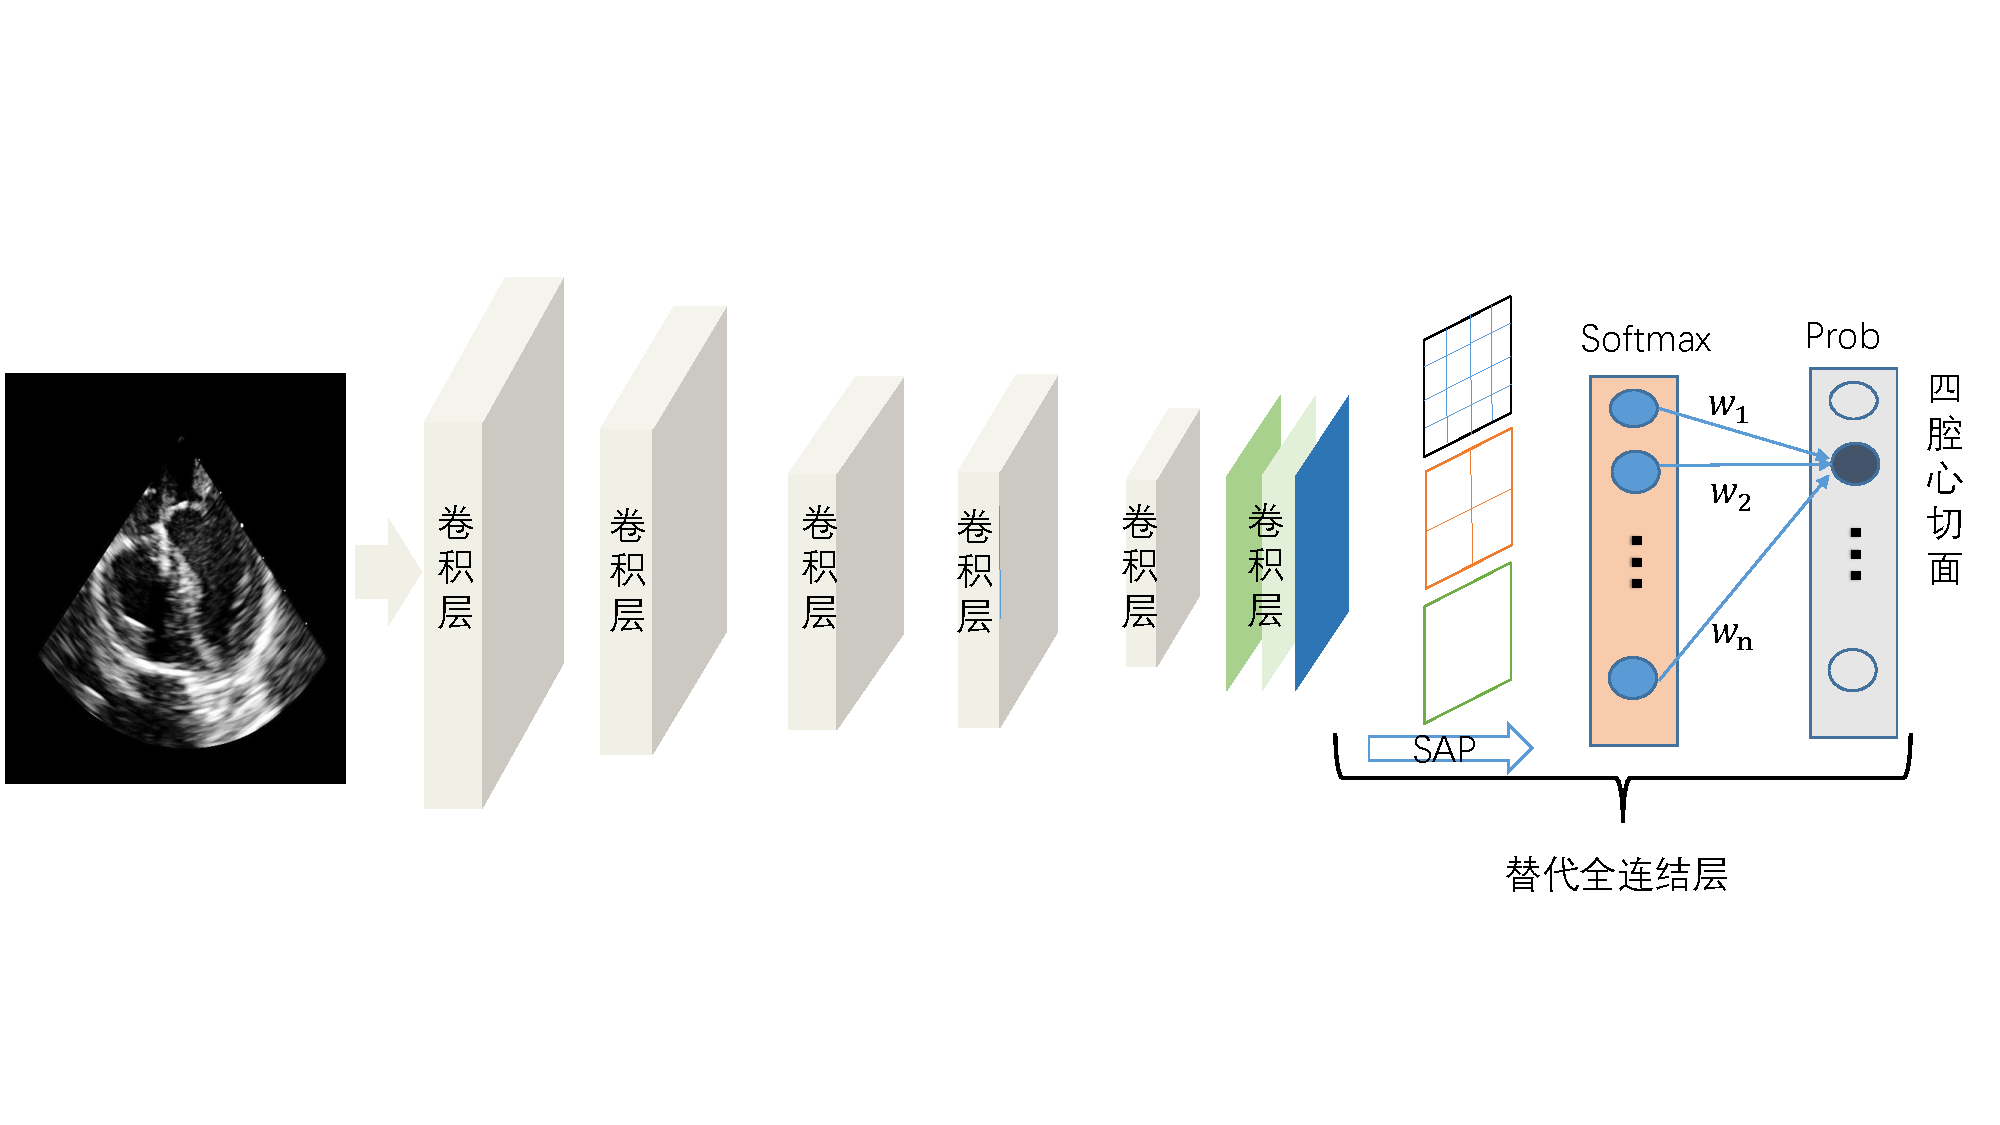
\includegraphics[trim = 30mm 0mm 30mm 0mm, clip, width=0.45\textwidth]{ch03_02}
    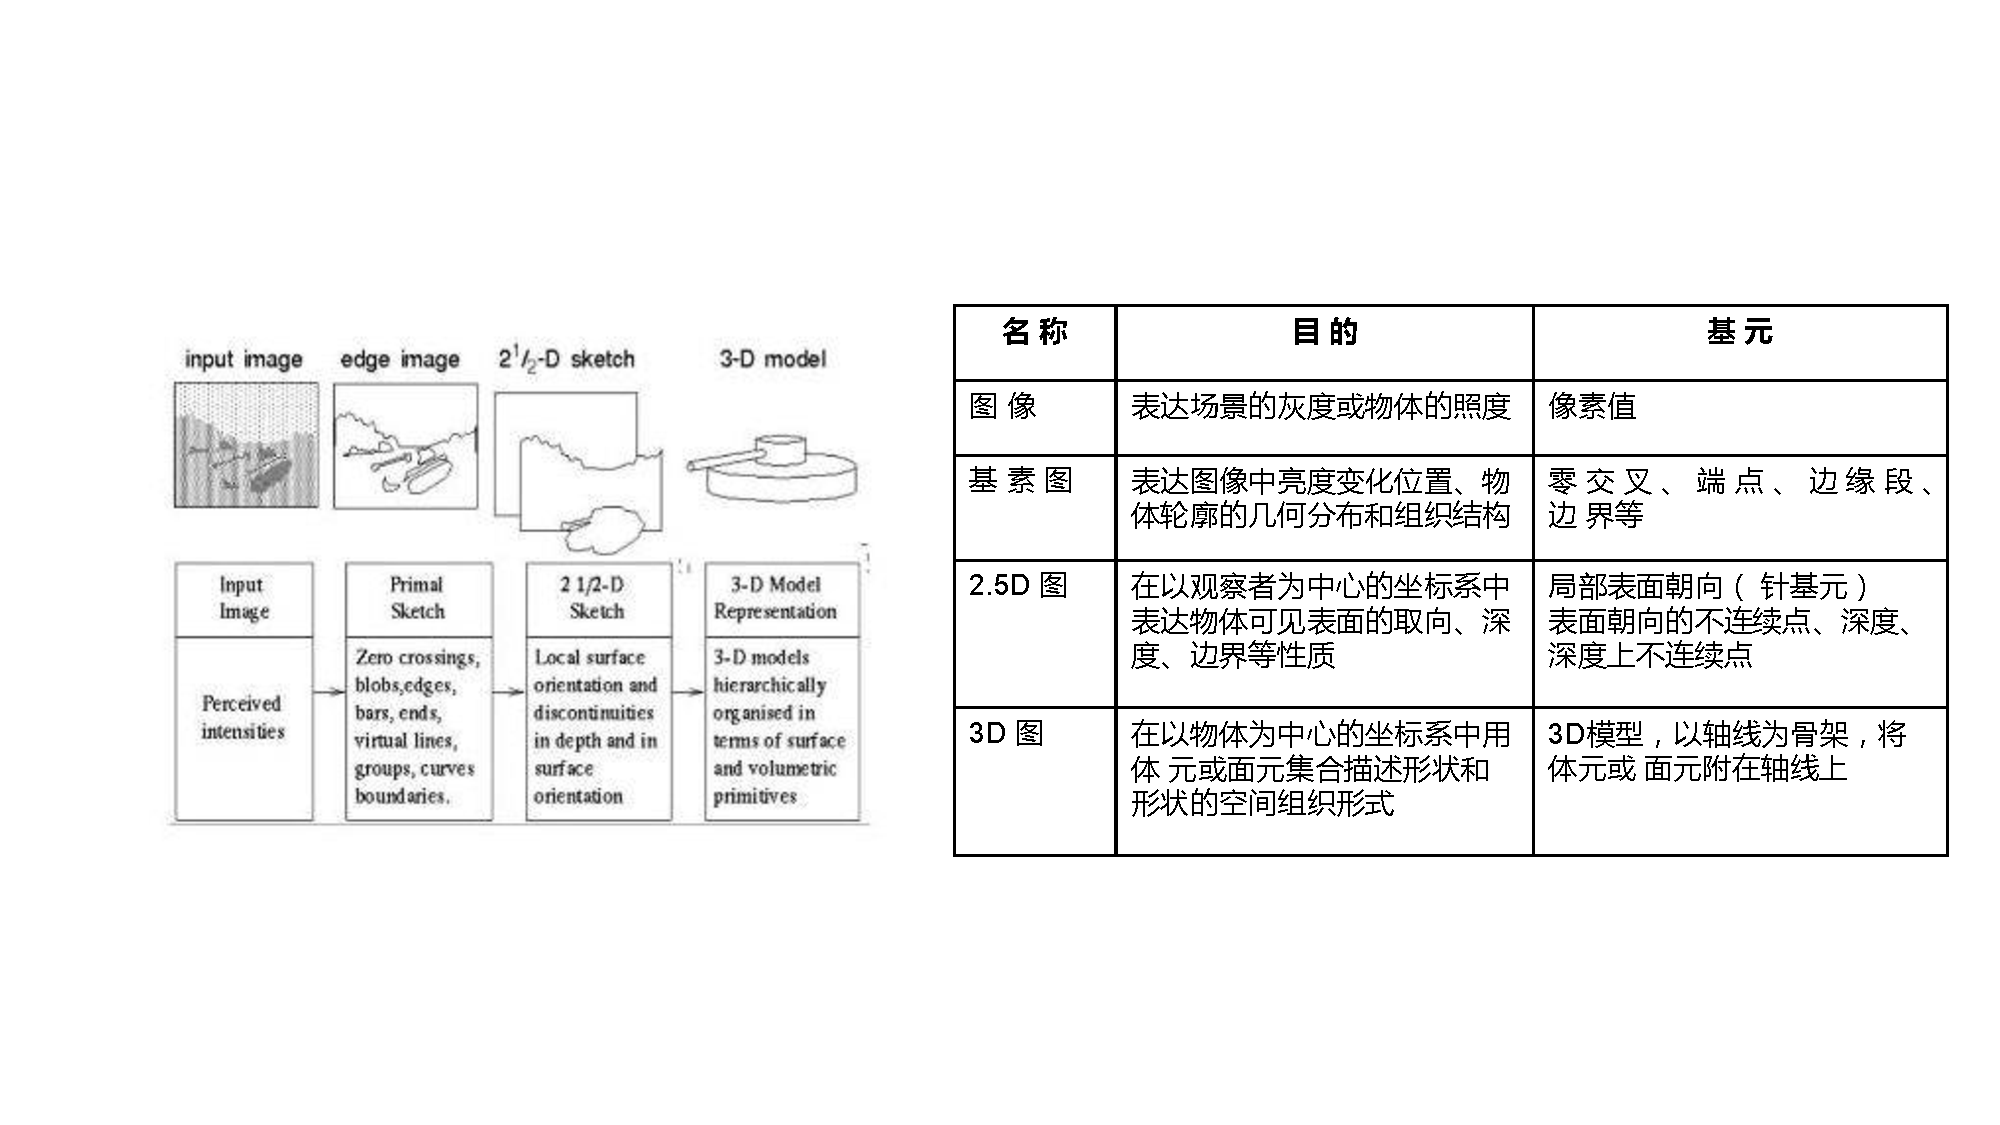
\includegraphics[width=0.85\textwidth]{ch01_01}
    \caption{David Marr视觉计算理论的分层结构示意图}
    \label{fig:ch01_01}
\end{figure}
    
从20世纪80年代开始,基于逻辑学和知识库推理的专家推理系统在人工智能领域大行其道,计算机视觉的理论方法论随之改变,Biederman在Marr的基础上提出组成识别理论(Recognition by Component Theory)。该理论认为通过把复杂对象解译(Image Parsing)为简单的部件形状,就可进行视觉统计模式匹配。Treisman等\cite{treisman1980a}提出特征融合理论(Feature Intergration), 认为视觉处理是一个以自下而上、局部交互作用的过程。Itti等\cite{Itti2005}提出适用于自然图像的高斯金字塔视觉注意机制模型模型。研究发现要让计算机理解图像,不一定先要恢复物体的三维结构。利用包括统计形变模型\cite{Cootes2004}以及能量泛函模型\cite{Kass1988},对图像进行解译(Image Parsing),将物体形状、颜色和纹理等先验特征进行统计模式匹配,寻找一个层次化、结构化的解释是计算视觉的核心问题。

\begin{figure}[!htbp]
    \centering
    %trim option's parameter order: left bottom right top
    %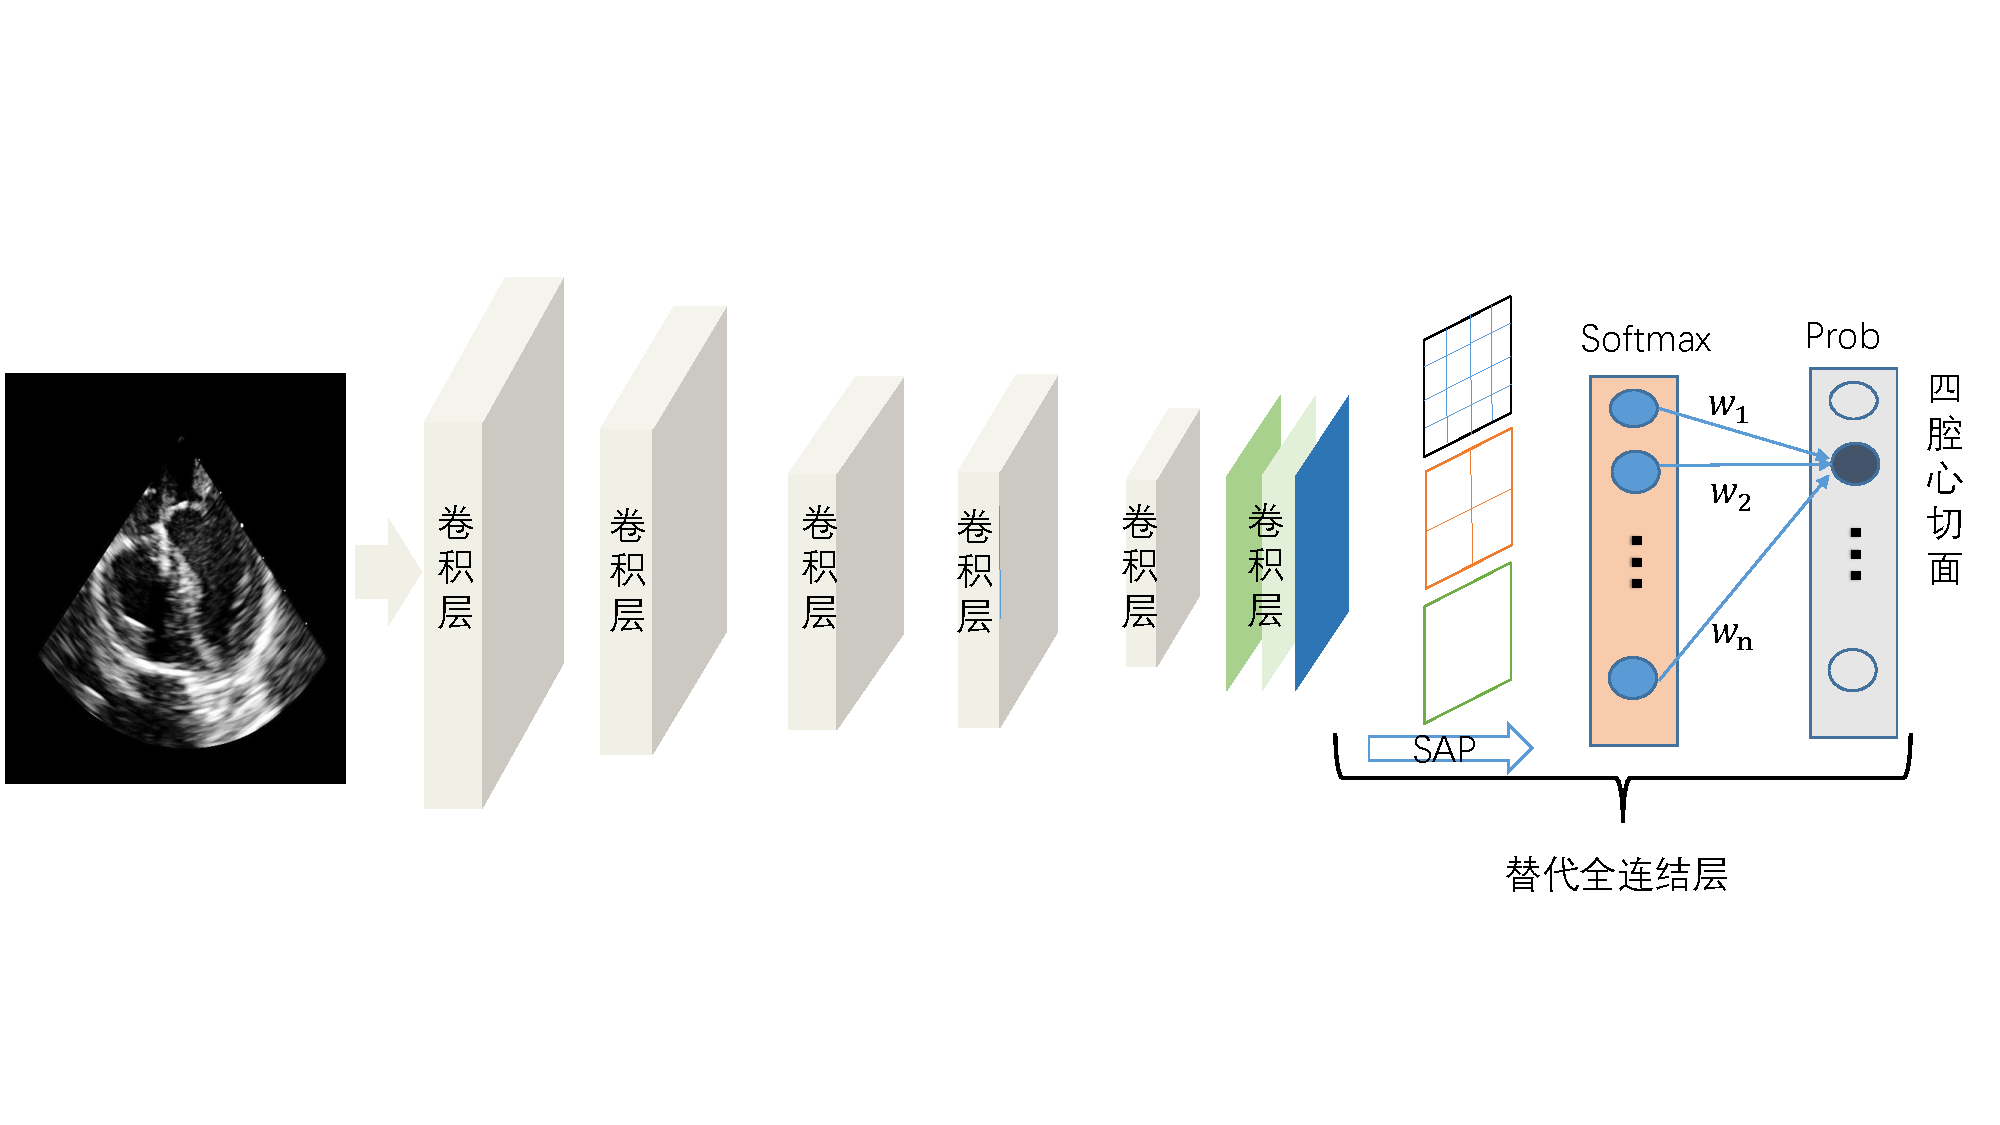
\includegraphics[trim = 30mm 0mm 30mm 0mm, clip, width=0.45\textwidth]{ch03_02}
    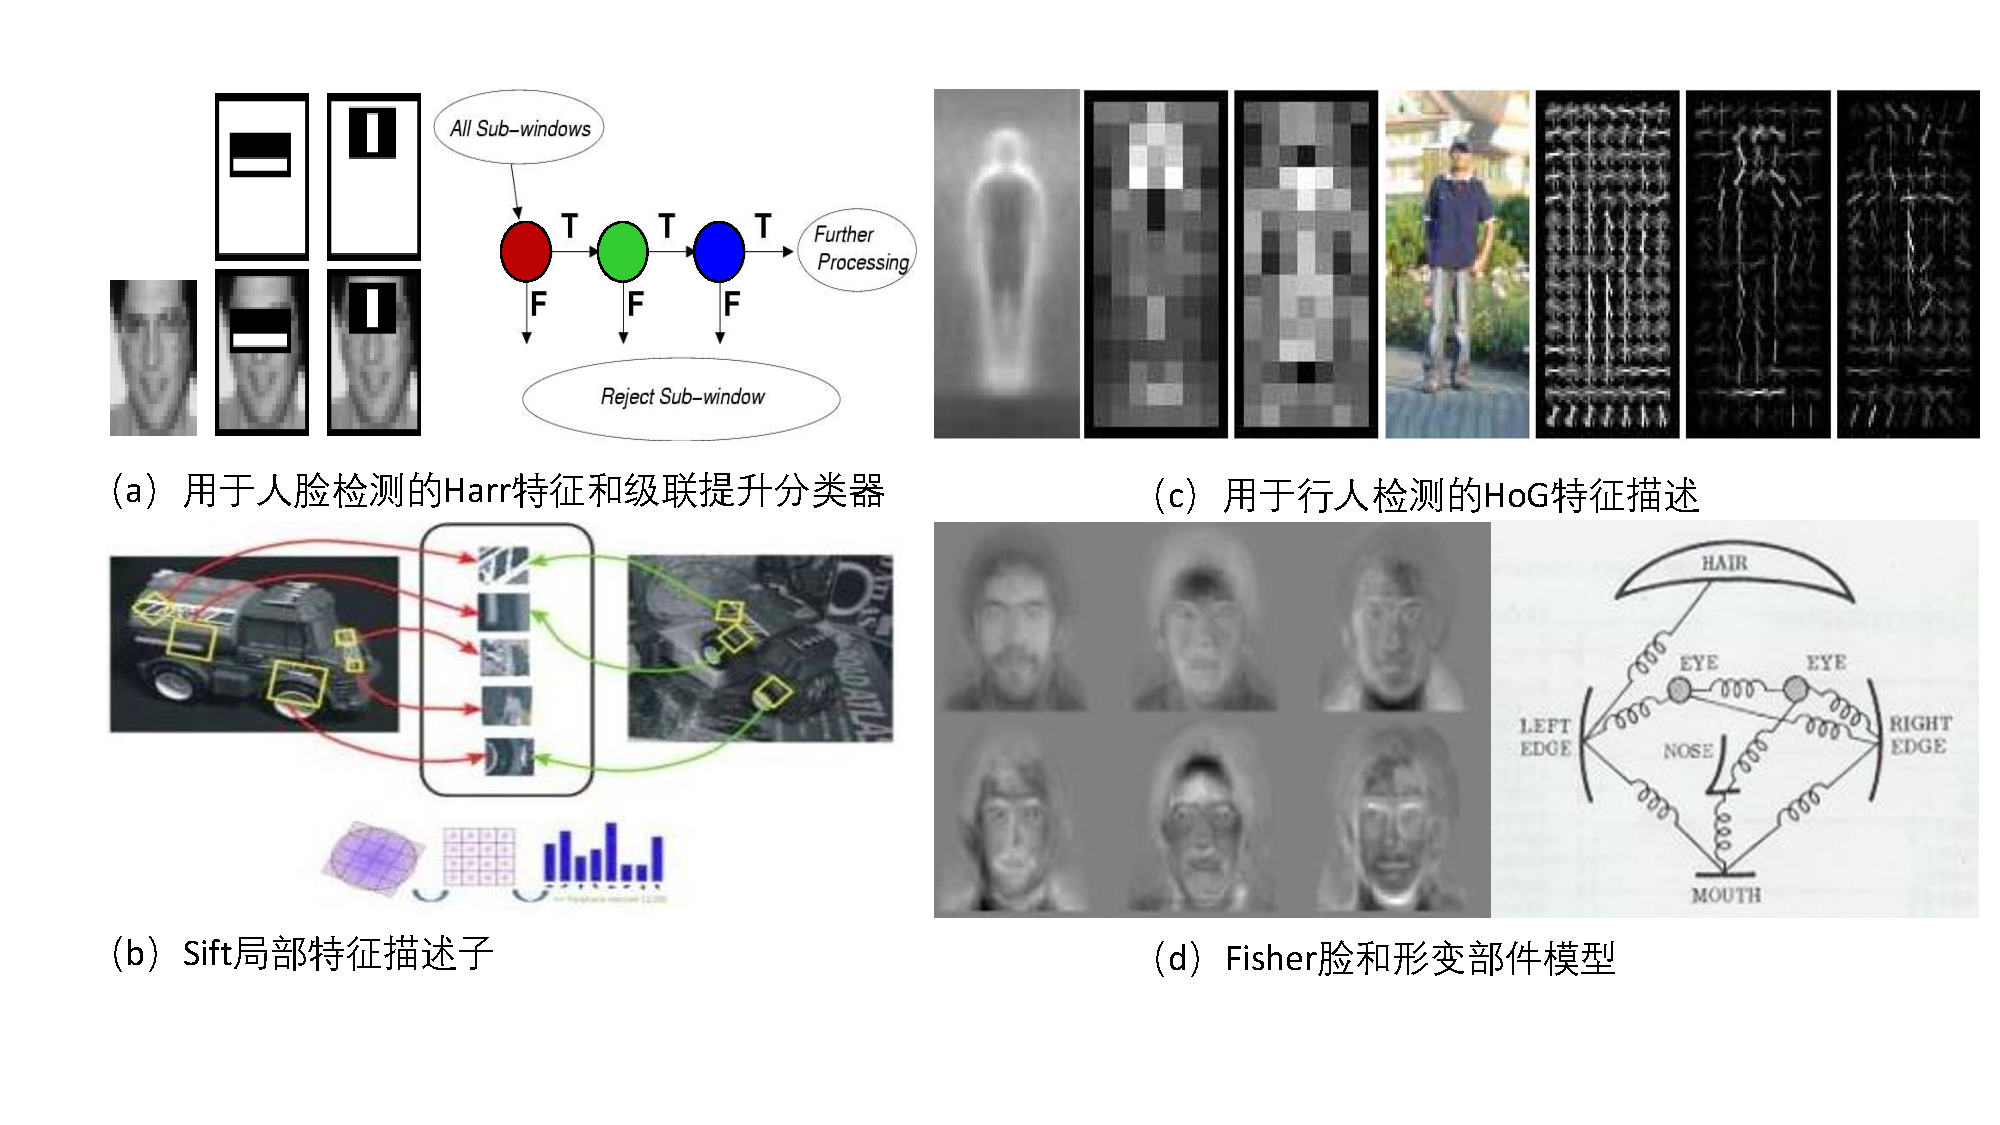
\includegraphics[width=0.85\textwidth]{ch01_02}
    \caption{局部特征结合机器学习的机器视觉代表性方法举例}
    \label{fig:ch01_02}
\end{figure}

进入新世纪后,互联网产生了海量图像数据,大规模数据集也随之出现,导致面向描述符的机器学习方法开始盛行,之前需通过规则、知识或统计模型设计形状、颜色、纹理等先验表征,易受额外影响不具有统计不变性,通过统计手段寻找能够刻画对象最本质的一些局部特征,其进展直接导致诸多应用的出现,如:图像搜索技术进入实用。目标识别领域涌现出空间金字塔(Spatial Pyramids)\cite{Lazebnik2006}、矢量量化(Vector Quantization)\cite{Yang2009b},以及在计算机视觉的各个阶段使用的各种机器学习工具。Lowe\cite{Lowe2004}提出旋转和尺度不变的局部特征描述符( Scale Inrariant Feature Transform,SIFT),改进后成为模式识别中的经典模型。Viola和Jones\cite{Viola2001}提出基于哈尔特征和级联Adaboost分类器人脸检测框架;Grauman等\cite{Grauman2005}发展了词袋模型(Bag of Word,Bow)用于图像物体识别;\cite{}提出方向梯度直方图(Hog)特征,利用变形部件模型结合支持向量机进行行人检测。因此,从完全由人类设计的系统转变为由使用计算机提取示例数据进行训练获得特征向量的的系统,计算机算法决定了高维特征空间中的最佳决策边界,设计此类系统的关键步骤是从图像中提取判别特征,该过程仍然是由人类手工设计完成的。

故合理的下一步就是让计算机自动从数据学习最佳特征表示,如图\ref{fig:ch01_03}揭示了手动设计特征的传统方法与自动提取特征的深度学习方法,模型(网络)由多层组成,将输入数据(例如图像)转换为输出(例如疾病存在/不存在),同时学习更高层次的特征。目前最成功的图像分析模型是卷积神经网络( convolutional neu- ral networks,CNN)。 CNN利用多层卷积滤波器来变换它们的输入。Fukushima早在1980年就提出有关CNN的工作,Lo等人于1995年应用于医学图像分析。LeCun提出了在手写数字识别领域的第一个成功的实际应用的LeNet。尽管取得了这些最初的成功,但在开发各种新技术以有效地训练深度网络之前,CNN的使用并没有形成势头。分水岭是Krizhevsky等人在2012年12月参加ImageNet识别竞赛挑战做出的贡献,提出AlexNet大幅度赢得了该竞赛。随后,使用相关但更深的架构取得了进一步的进展\cite{}。在计算机视觉各个任务领域,深度卷积神经网络现在已经成为首要选择的技术。
\begin{figure}[!htbp]
    \centering
    %trim option's parameter order: left bottom right top
    %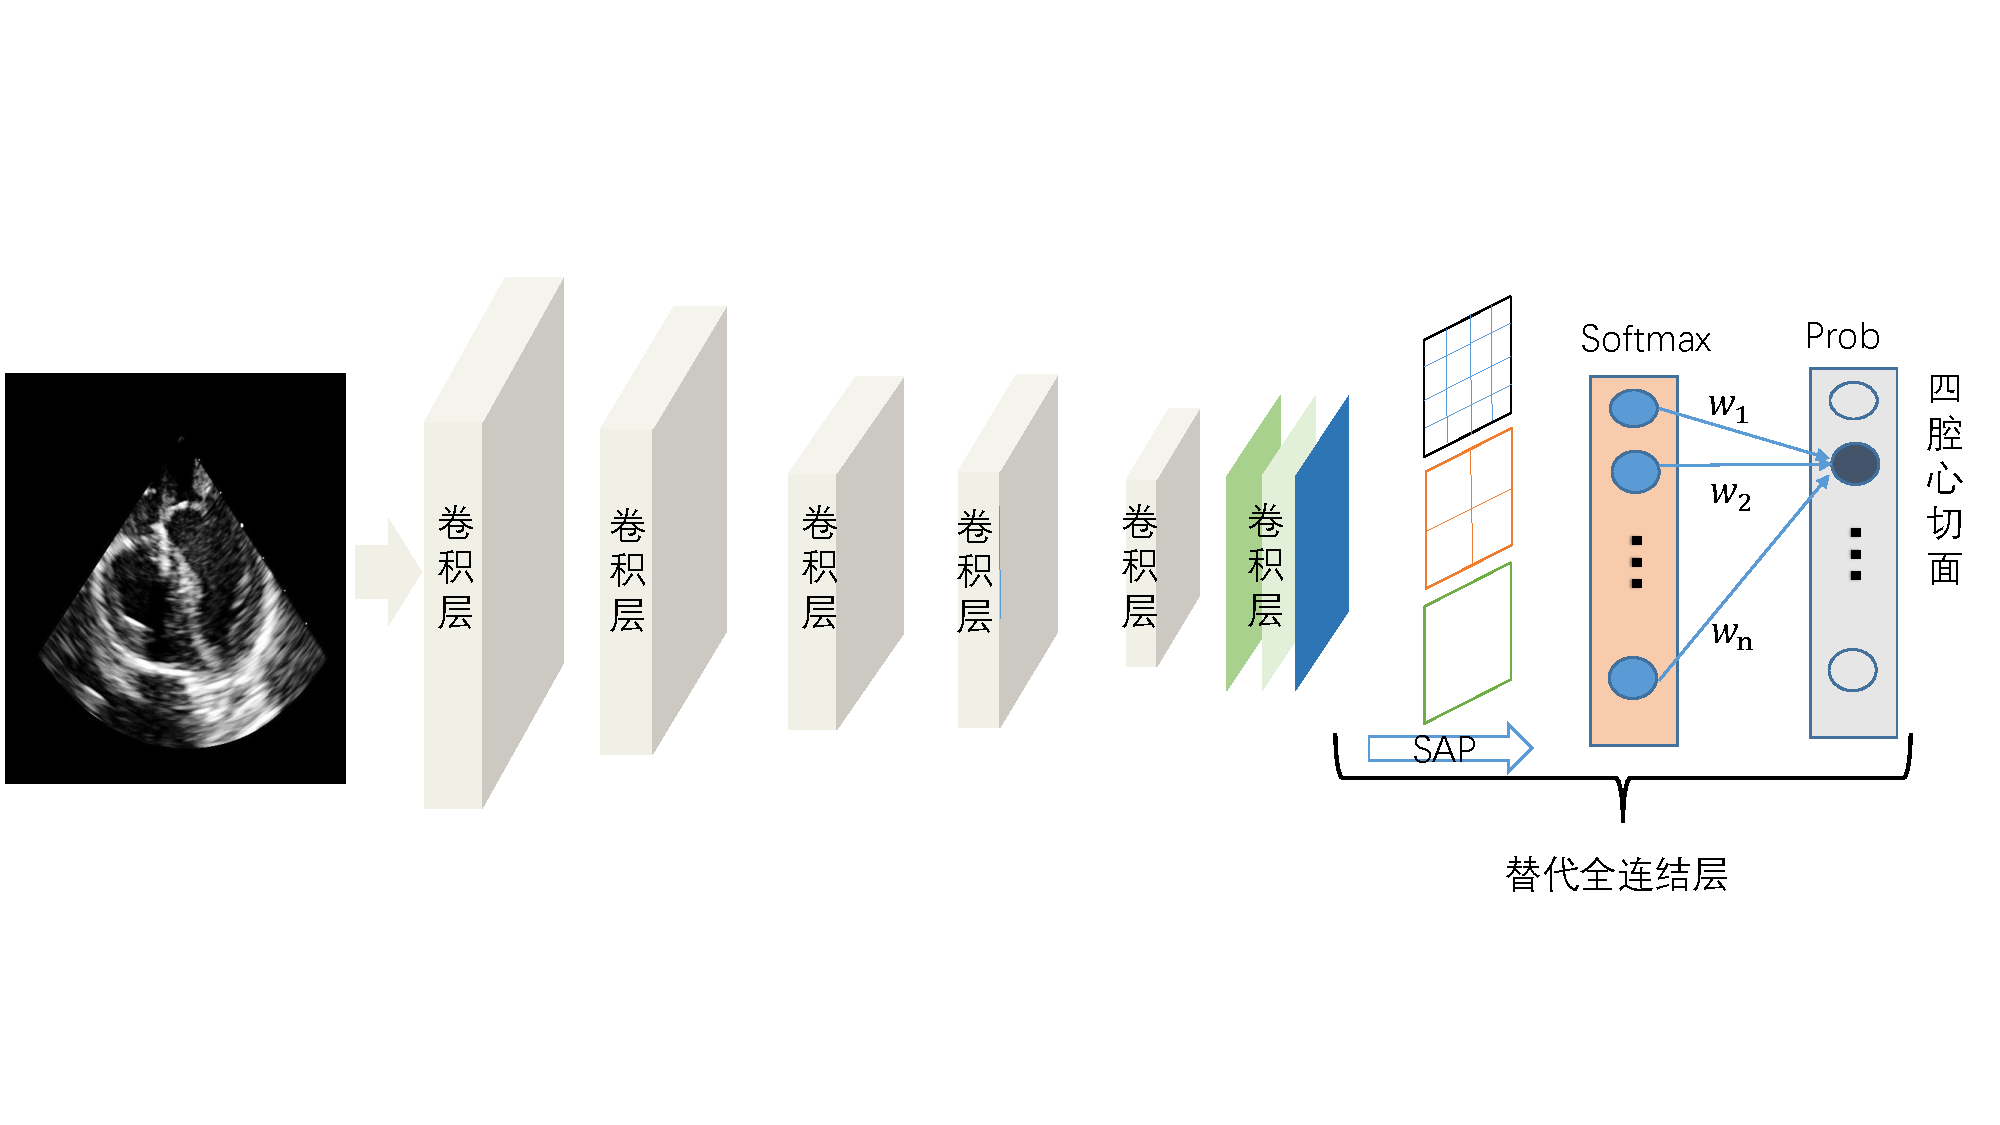
\includegraphics[trim = 30mm 0mm 30mm 0mm, clip, width=0.45\textwidth]{ch03_02}
    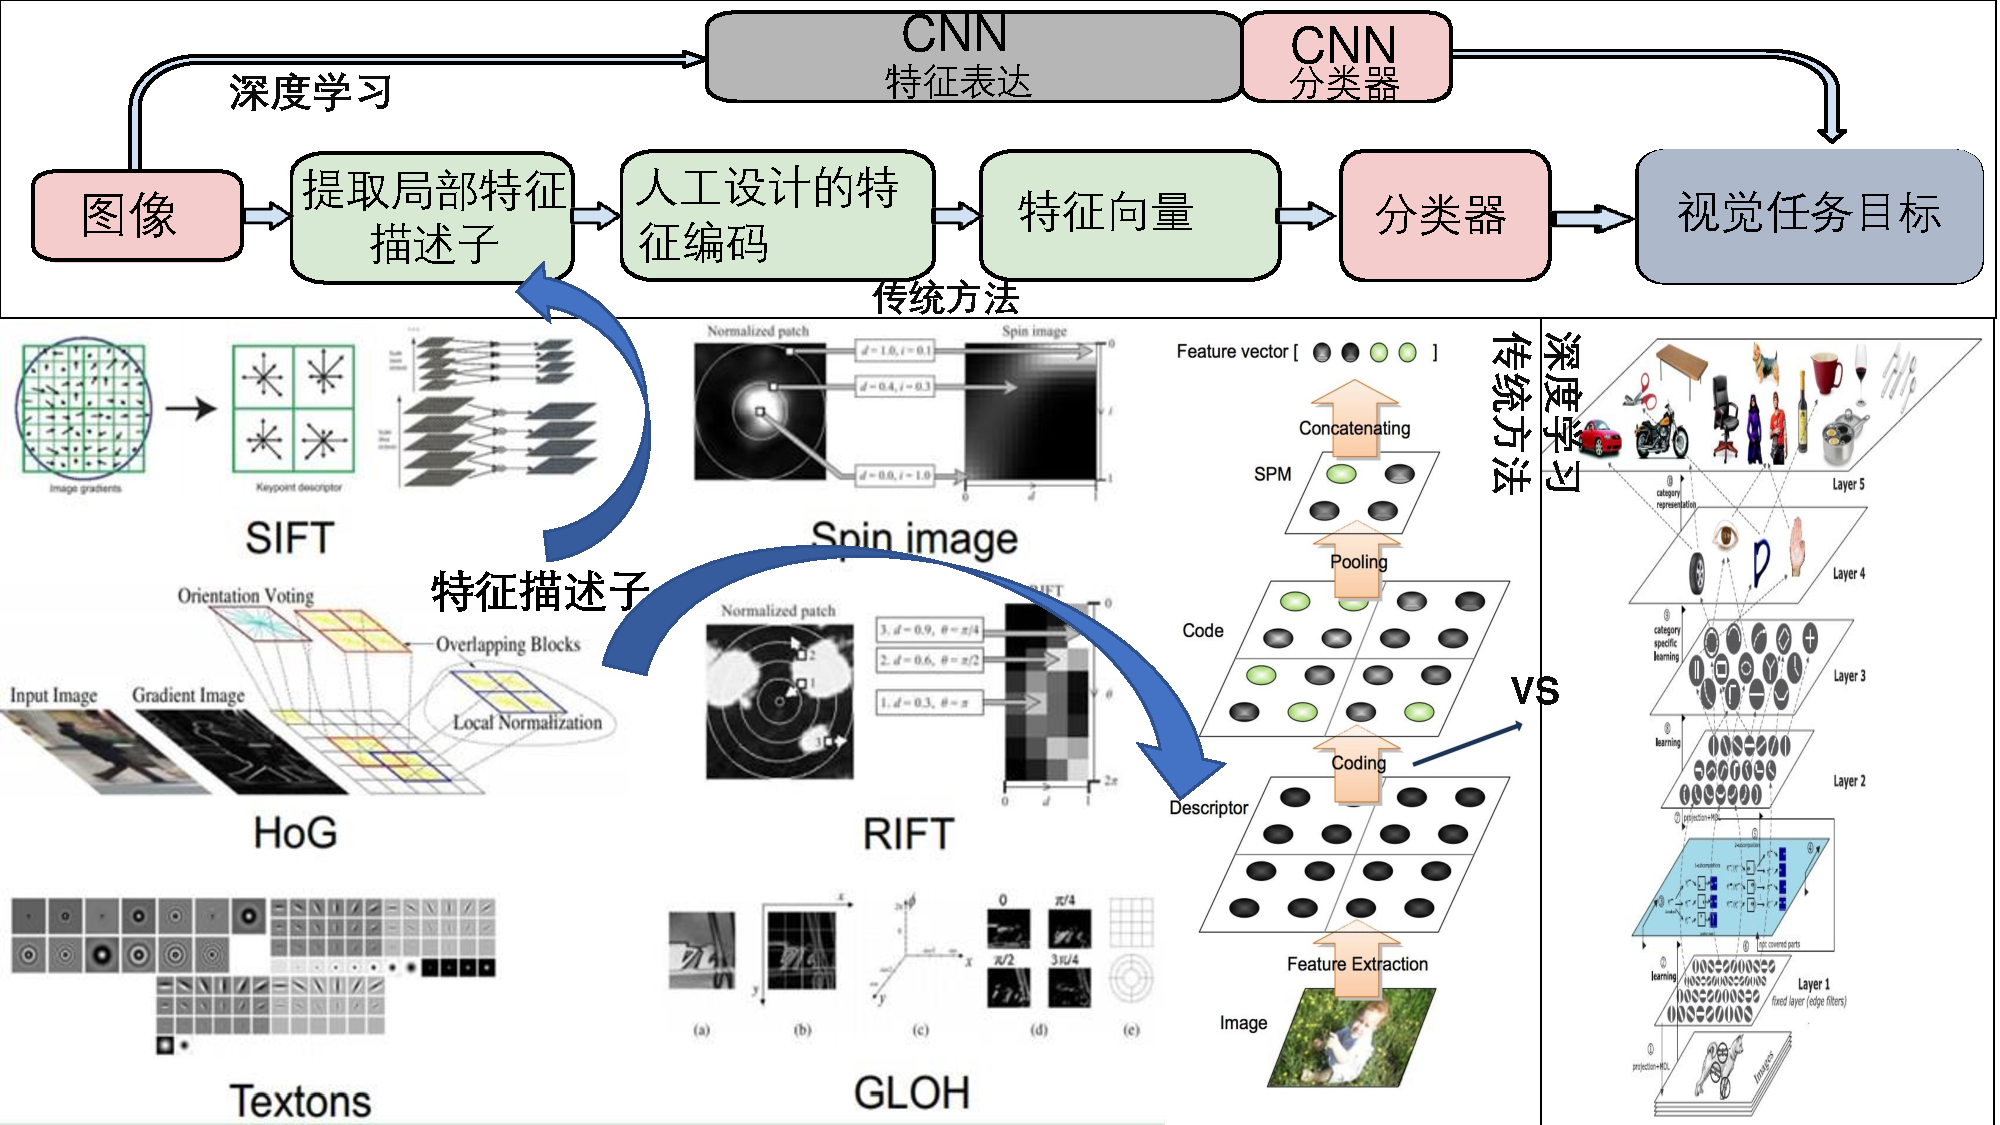
\includegraphics[width=0.85\textwidth]{ch01_03}
    \caption{传统图像识别方法与深度学习方法对比}
    \label{fig:ch01_03}
\end{figure}

另外一些研究者从模拟生物视觉机制出发,通过对感受野、注意机制、颜色特性和光流等方面进行计算机视觉研究。Hubel和Wiesel\cite{Hubel1962Receptive}对猫视觉皮层细胞的信息处理模式做了深入研究,提出视觉感受野(Receptive Field)概念,进一步发现了视觉皮层通路中对于信息的分层处理机制。{Riesenhuber等\cite{Riesenhuber1999}[26]首次从生物学的角度上模拟建立分层的视觉处理模型(Hierardical Model and X, HMAX),其模型与文献\citepns{Itti2005}中的模型类似。 Berthold等\cite{Horn1981}认为人类感知不是对视网膜上降采样图像的解释,而是对光学排列和流动的直接感受体验,提出光流(Optical Flow)用于描述图像灰度的表面活动形式,即获取运动场得到丰富的场景运动和场景结构等信息。

另外一些研究者从模拟生物视觉认知机制出发,McClelland和Pitts等[43]依据神经元连接方式提出神经元模型MP ,相关节点单元(Node)是最小的加工单元,节点之间通过通过兴奋和抑制两种连接方式联结成网络,利用“Hebb规则”的学习机制,指出神经元在不同时刻需具有变化的强度激活值(Activation Value)。该理论也成为在语言学中风靡的连接主义理论的代表性理论。Rosenblatt提出了由单层神经元组成的感知机(Perceptron)来完成线性分类任务;Fukushima 提出了神经网络多层的结构,但是并没有提出如何学习这个结构;Rumelhar 和 Hinton等人根据求导的链式法则提出了反向传播(Backpropagation,BP )算法,解决了多层神经网络所需要的复杂计算量问题。Hopfield提出利用能量函数的概念来研究一类具有固定权值的循环神经网络的稳定性并付诸电路实现,它保证了向局部极小的收敛,可以解决一大类模式识别问题,还可以给出一类组合优化问题的近似解。lecun针对图像领域提出了lenet。萨纳内等[4]应用CNNs从乳房X线照片中提取含有活检证实的肿块或正常组织的ROI;也被应用于肺结节检测[5];用于检测乳房X线照相术中的微钙化[6]。在医学图像处理中,GPU首先被引入用于分割,重建和配准,然后被用于机器学习[9],[10]。 

\begin{figure}[!htbp]
    \centering
    %trim option's parameter order: left bottom right top
    %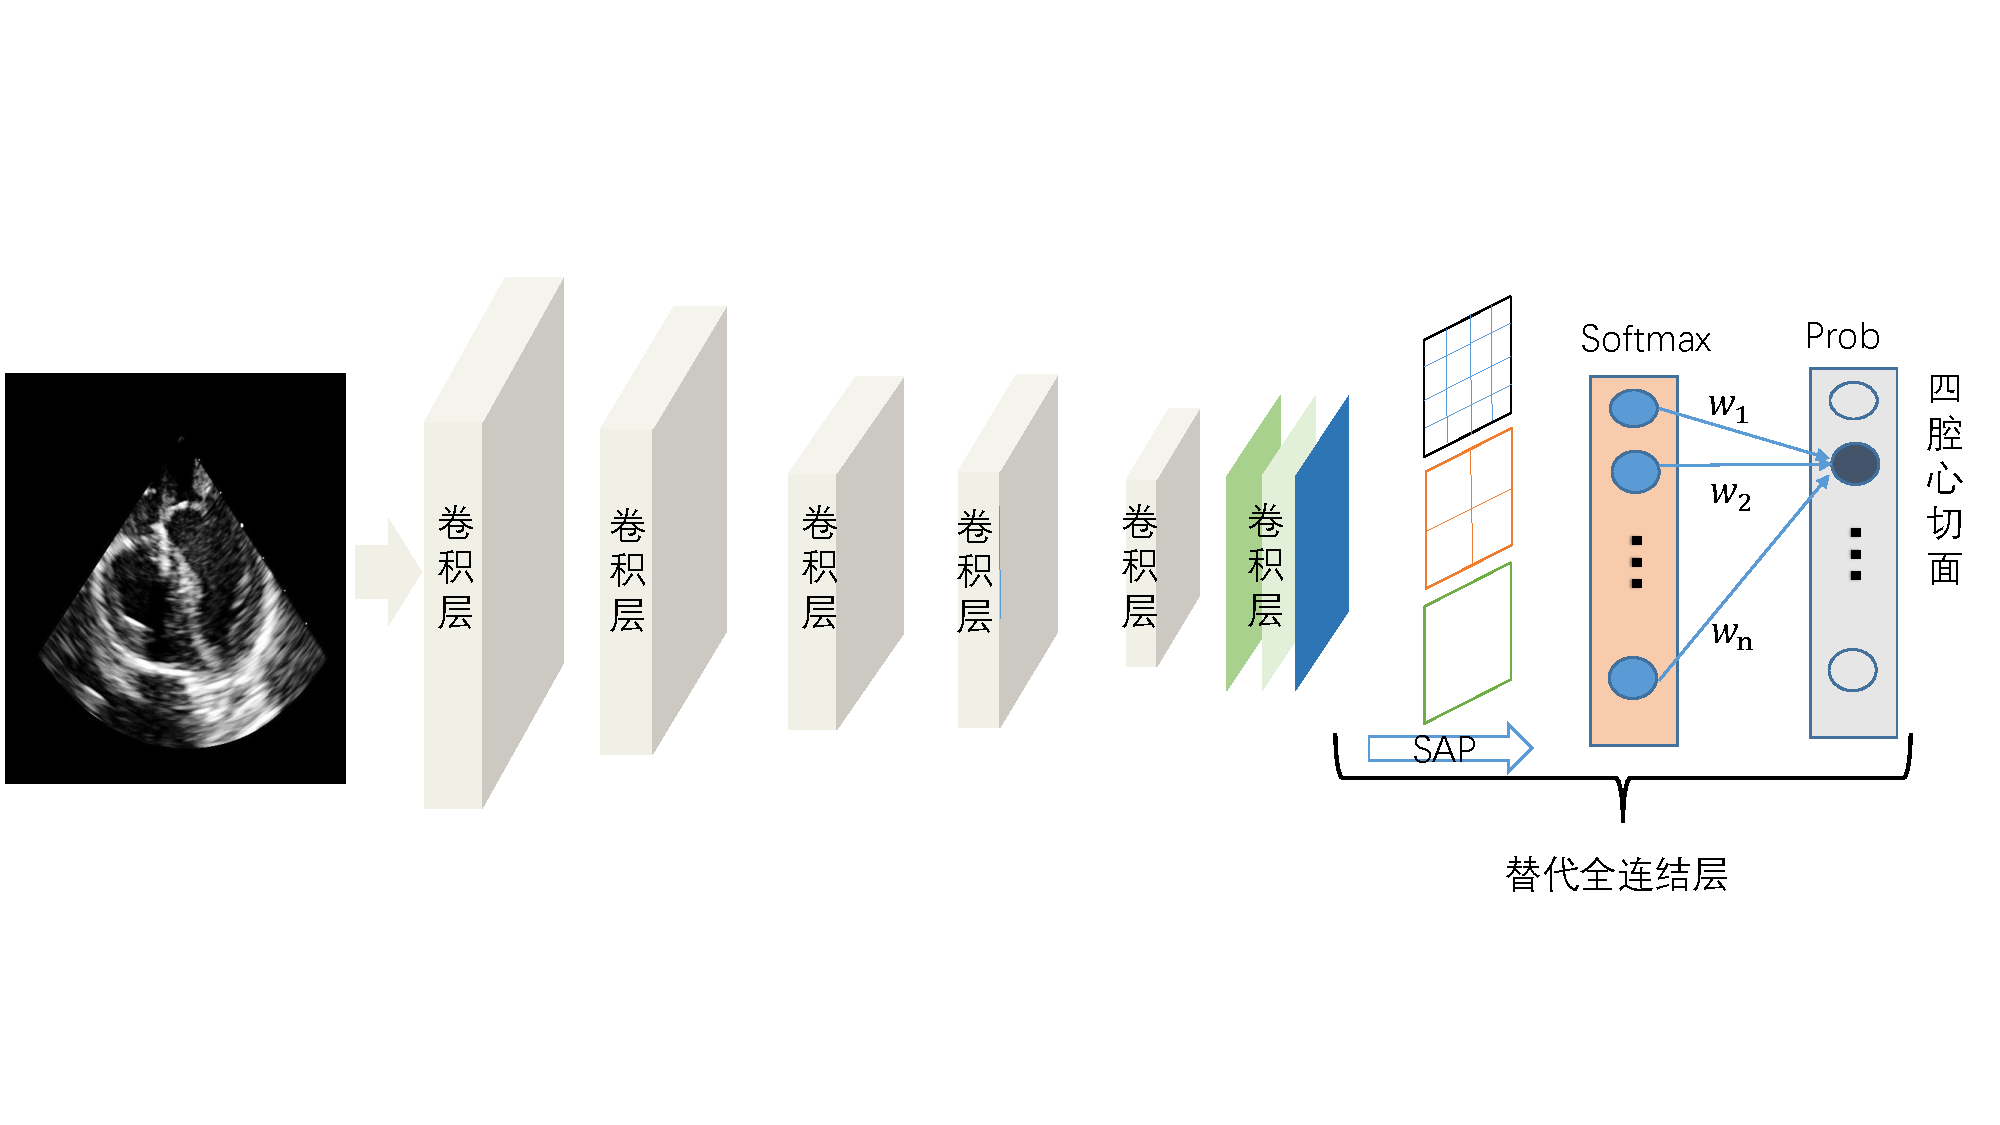
\includegraphics[trim = 30mm 0mm 30mm 0mm, clip, width=0.45\textwidth]{ch03_02}
    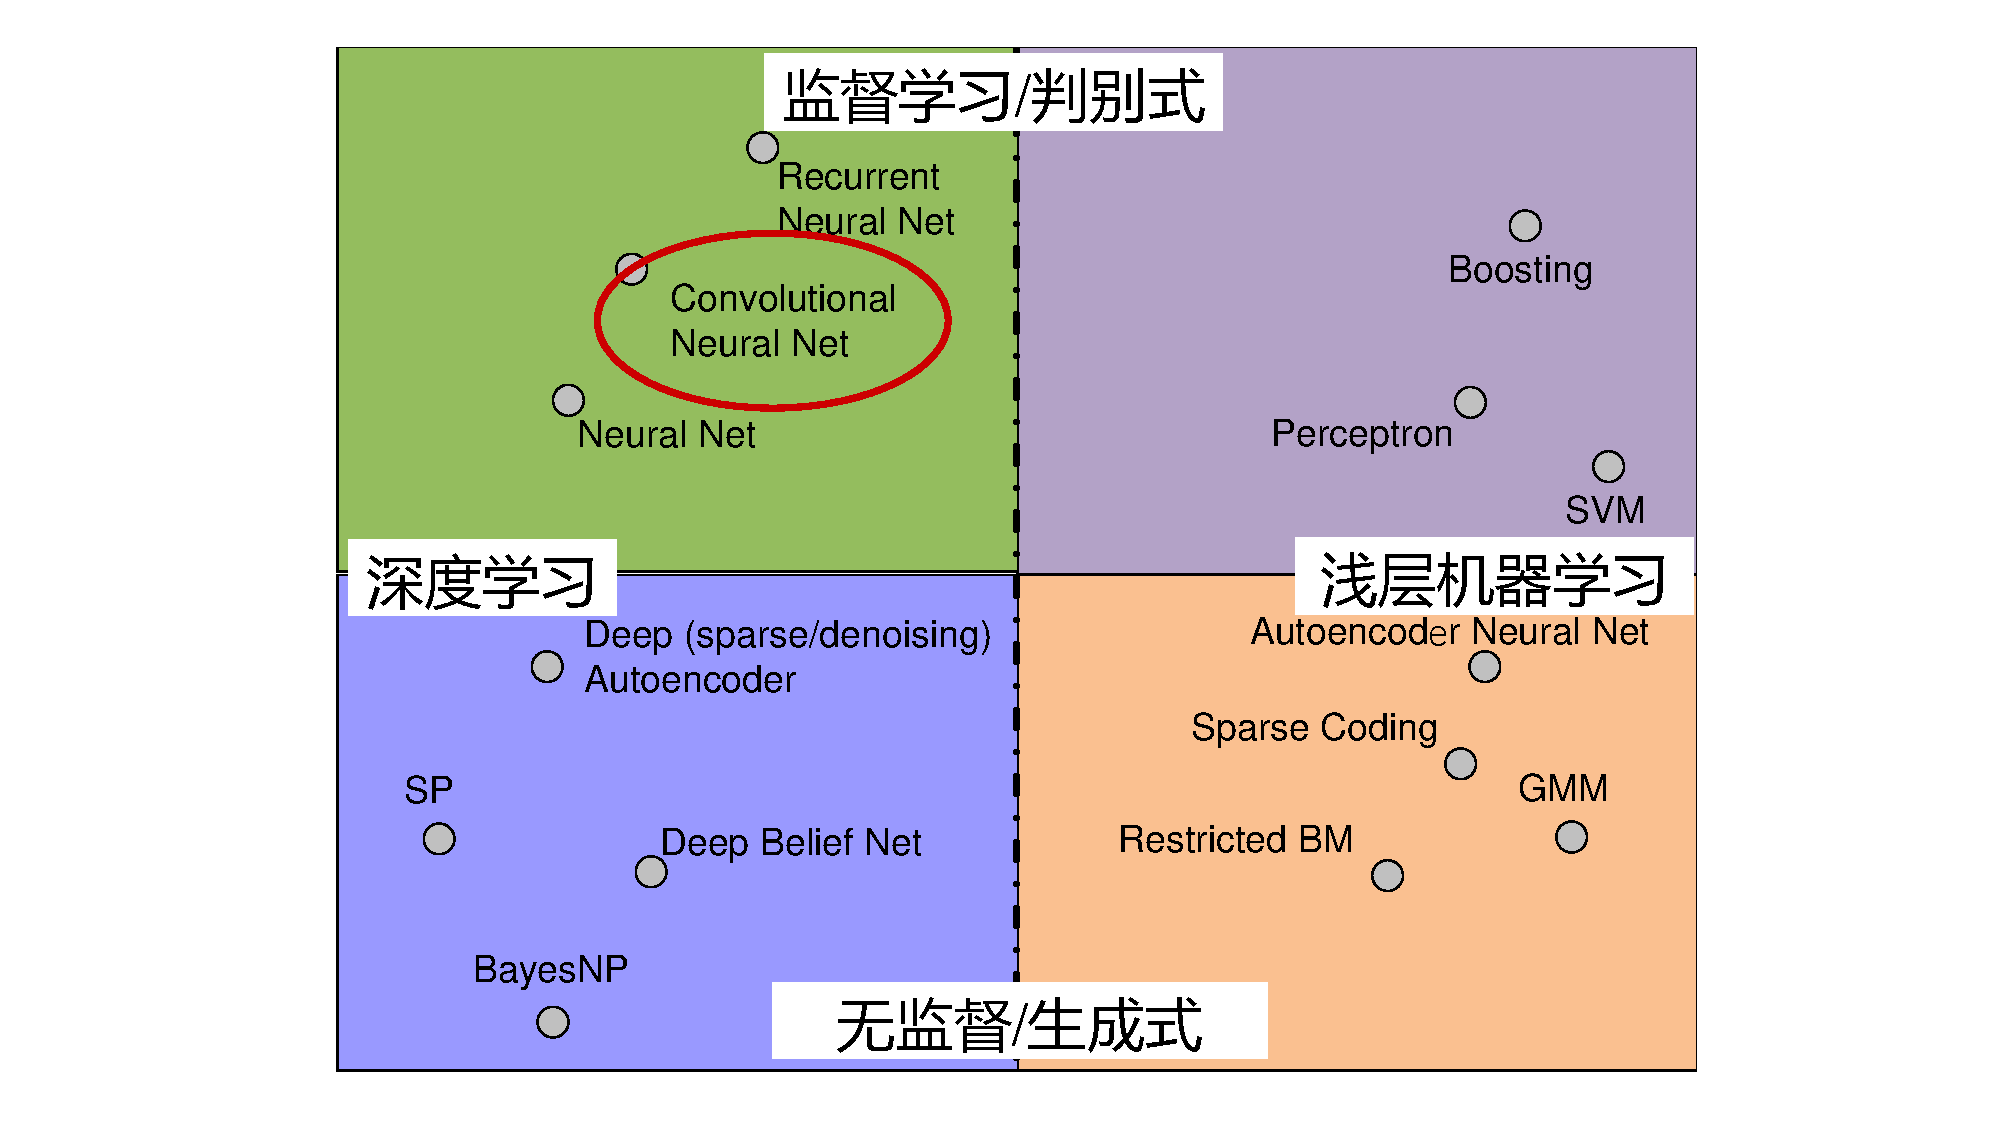
\includegraphics[width=0.85\textwidth]{ch01_04}
    \caption{统计机器学习方法分类总结}
    \label{fig:ch01_04}
\end{figure}

\subsection{深度学习在医学图像分析应用的研究现状}


从使用手工设计特征转换到从数据中学习特征,医学影像分析界业已注意到这些关键进展,在AlexNet突破之前,依据模型结构深浅和监督与非监督四个维度度现有机器学习方法进行归类\ref{fig:ch01_04},神经网络和深度学习背后的基本理念如上节所述,受限于计算力起初的神经网络通常只有几层,由于理论分析的难度大,训练方法又需要很多经验和技巧,这个时期浅层人工神经网络反而相对沉寂。相继提出了各种各样的浅层机器学习模型,如支持向量机(Support Vector Machines,SVM)、 集成学习(Boosting)、稀疏编码(Sparse Coding)等,这些模型基本上视作只有有一层隐层节点(如SVM、Boosting)的浅层神经网络,这些模型无论是在理论分析还是实际应用于医学图像分析中都获得了不小的成功,特别是用于检测异常情况,而且还用于分割等相关领域。 尽管有这些发展,但检测的假阳性率相对较高。

自2006年hiton提出深度学习以来,方兴未艾的深度学习真正改变了计算机视觉之前的定义,它正在成为计算机视觉领域最优的机器学习工具。特别是卷积神经网络已被证明是广泛的计算机视觉任务的强大工具。世界各地的医学图像分析团队正在迅速进入该领域,并将CNN和其他深度学习方法应用于各种各样的应用,令人鼓舞的结果正不断涌现,如图\ref{}, 从左上到右下依次为:乳房X线图像质量分类\cite{Sickles2006Use},大脑病灶分割(\cite{Abr2016Improved}),气道树分割中的泄漏检测 \cite{Charbonnier2016Improving},视网膜病变分类(Kaggle糖尿病视网膜病变图像)\cite{Grinsven2016Fast},前列腺分割, 结节分型,淋巴结中的乳腺癌转移检测,皮肤病变分类\cite{Esteva2017Dermatologist}和来自Yang等人\cite{Yang2016Cascade}的最新X射线骨骼抑制技术。文献\cite{Litjens2017Asurvey,Shen2017a,Greenspan2016}对深度学习应用于医学图像分析做了专门综述。

\begin{figure}[!htbp]
    \centering
    %trim option's parameter order: left bottom right top
    %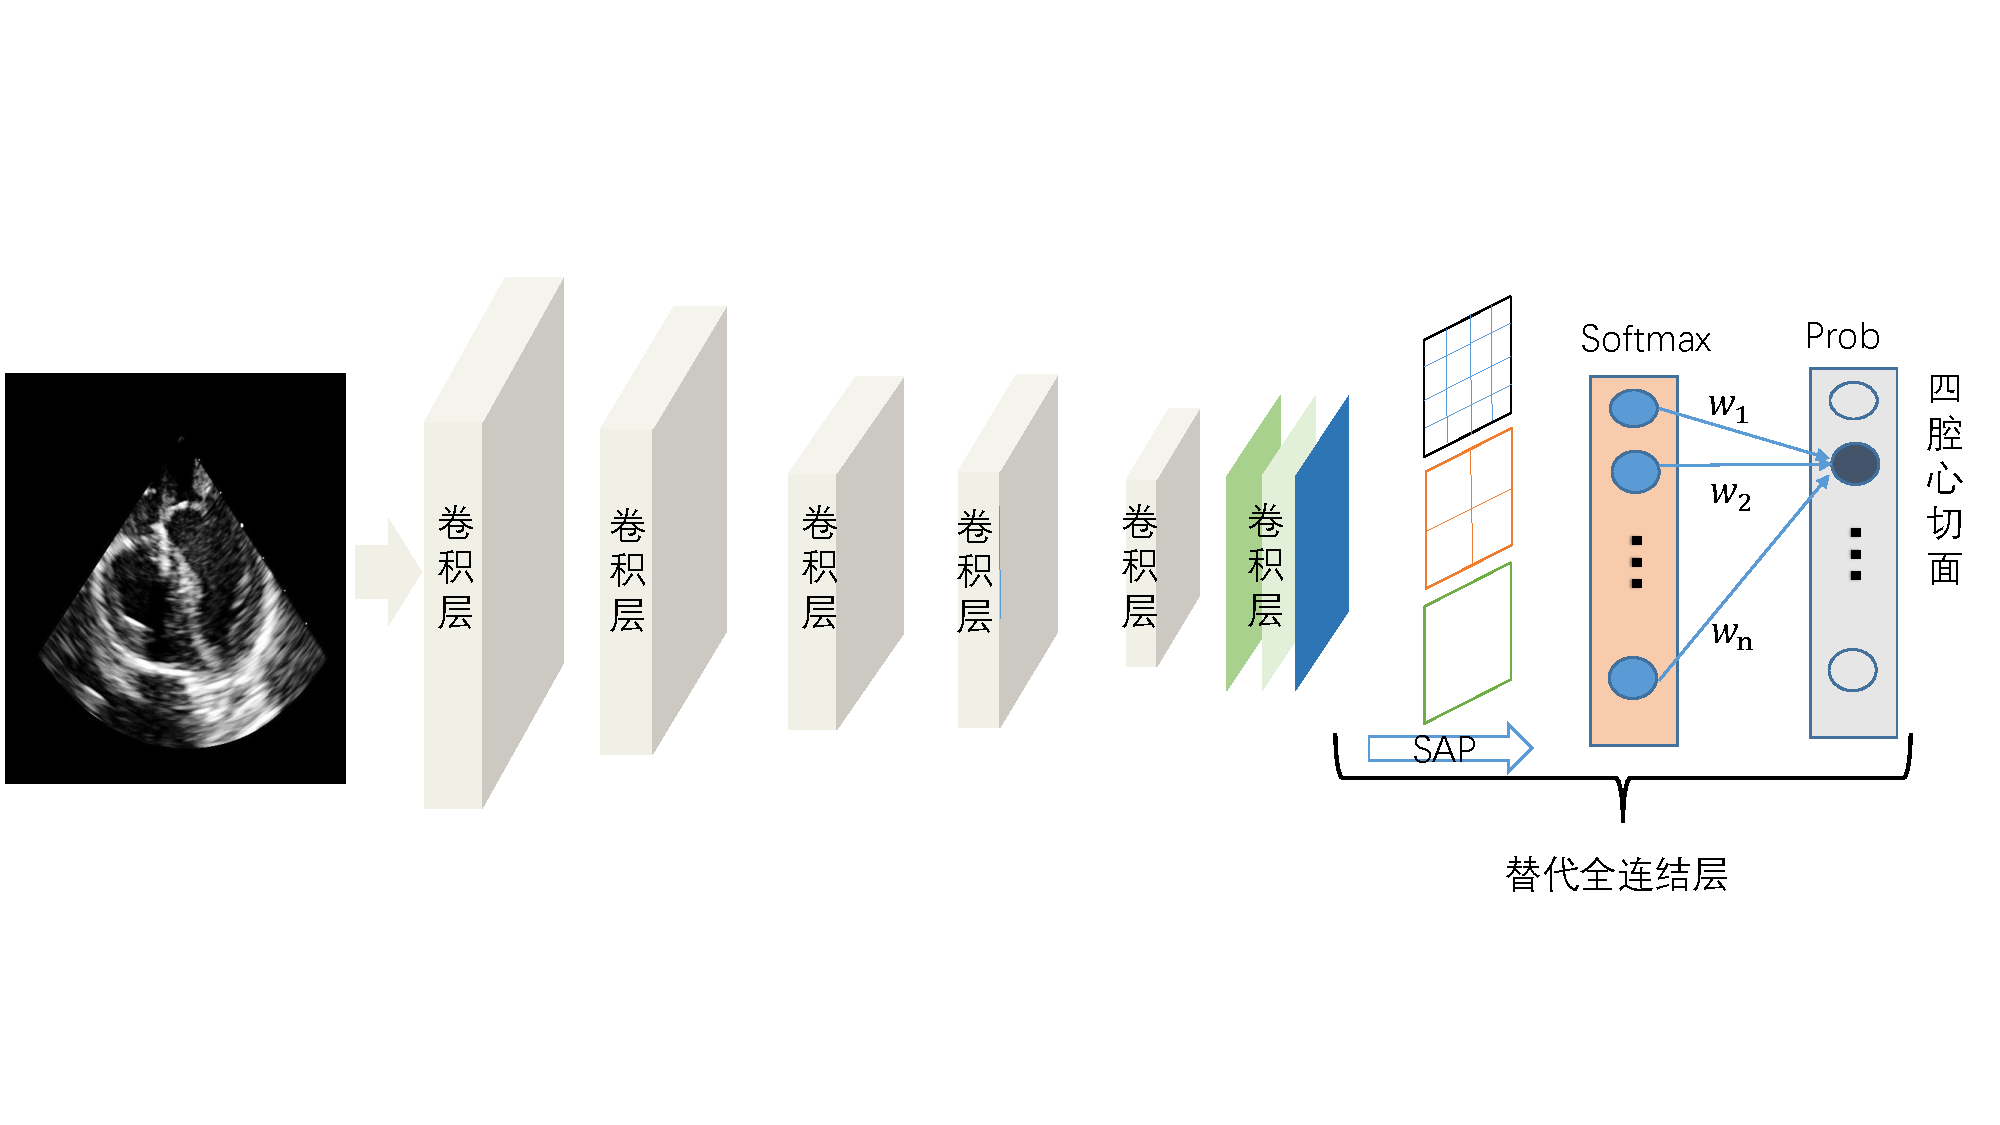
\includegraphics[trim = 30mm 0mm 30mm 0mm, clip, width=0.45\textwidth]{ch03_02}
    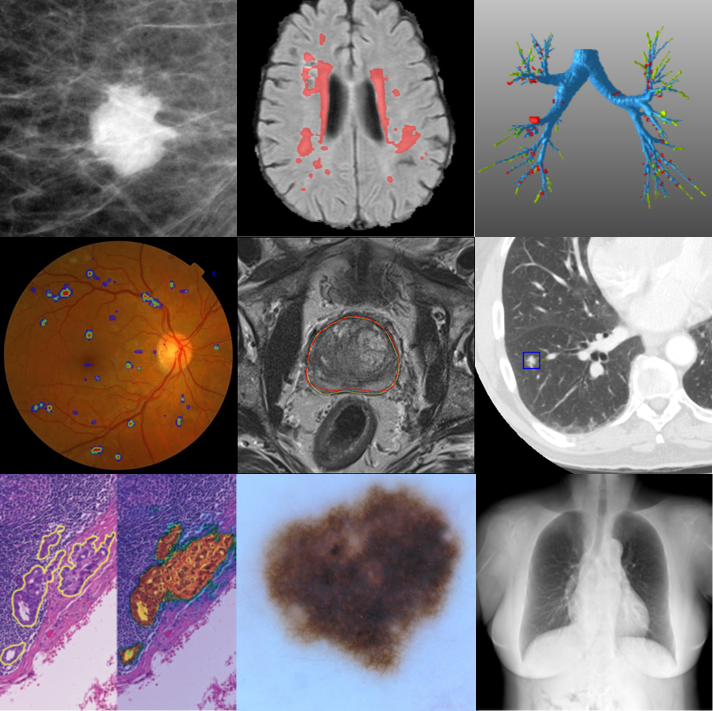
\includegraphics[width=0.85\textwidth]{ch01_05}
   \caption{一些医学影像学应用深度学习取得了最优成果集图}
   \label{fig:ch01_05}
\end{figure}

\subsubsection{分类识别}

图像识别分类是深度学习对医学图像分析做出贡献的首要领域之一,尤其是对自然图像进行预训练的CNN已经显示出惊人效果,在一些任务中超过了人类。相关研究表明可以调整CNN以利用医学图像的内在结构,Chen等\citep{Chen2015}利用CNN结合领域知识,在胎儿超声心动图标准切面的自动识别问题中取得良好的识别效果。Bar等\citep{Bar2015Chest}利用自然图像训练的模型对胸腔X-射线图像进行特征提取并结合全局特征\citep{Oliva2001}得到最优检测结果。Margeta等\citep{Margeta2015}针对心脏核磁共振图像利用微调迁移从自然图像学习的模型。总之与图像分类相比,医学对象分类较少使用预先训练的网络,这主要是由于当前卷积网络较难结合上下文或三维信息。

\subsubsection{病变检测} 

计算机辅助检测在医学图像分析领域是一个非常成熟的任务,解剖对象定位(空间或时间),例如器官或标记,一直是分割任务或治疗计划和干预的临床工作流程中的重要预处理步骤。传统CAD\cite{Van2011Computer}通过监督方法或经典的图像处理技术(如滤波和数学形态学)检测候选区域,各阶段通常是分离开的,并常由手工设计的特征来描述,分类器用于将特征向量映射到实际病变的概率。深度学习采用直接以一个以候选病灶为中心的图像数据区域进行操作,训练一个端到端的CNN。如利用深度卷积网络进行显微镜图像中细胞检测\citep{Akram2016}、结合深度全卷积网络的MRI心室检测与分割\citep{Emad2015,Tran2016a}和超声图像解剖结构的检测\citep{Chen2016i}。Roth等人\cite{Roth2016}使用CNN改进三个现有的CAD用于CT结肠镜检查的结肠息肉,体部CT上的硬化性脊柱转移以及体部CT上的肿大淋巴结的检测。
医学成像中的定位通常需要解析3D体积,为了用深度学习算法解决3D数据解析,已经提出了几种将3D空间视为二维正交平面组合的方法,Setio等人\cite{Setio2016Pulmonary}检测在3D胸部CT扫描中的肺结节,使用不同CNN的组合来对每个候选区域进行分类。相关综述请参考文献\cite{Shin2016}。总之与分类识别问题类似,直接解决特定于对象检测的问题,如类不平衡/硬阴影挖掘或图像的有效像素/体素处理仍是个挑战。

\subsubsection{分割和形状建模}

医学图像中的器官和结构的分割允许定量分析与体积和形状有关的临床参数,它往往是计算机辅助检测的第一步。例如心脏或大脑分中,分割的任务通常被定义为识别组成感兴趣对象的轮廓或内部的体素集。分割是应用医学成像深度学习的论文中最常见的主题,因此也在深度学习方法学中广泛应用,包括开发独特的基于CNN的分割体系结构以及应用RNNs。 

这些新型CNN架构中最常用的是由Ronneberger等人\cite{Ronneberger2015}提出的U-net,将上采样和下采样层的组合,将它们与反卷积和反褶积层之间的所谓跳跃连接相结合,从而直接产生分割图。Milletari等人(2016b)提出了一种称为V-net的U-net架构的三维变体。RNN最近在分割任务中变得越来越流行。例如,Xie等人(2016b)使用空间RNN在组织病理学图像中分割肌束膜。 Stollenga等人。 (2015)首次在6个方向上使用带有卷积层的3D LSTM-RNN。安德马特等人(2016)使用3D RNN和门控循环单元来分割脑MRI数据集中的灰质和白质。陈等人。 (2016d)将双向LSTM-RNN与2D U-net-like-体系结构组合以在各向异性3D电子显微镜图像中分割结构。此外,基于深度学习的特征点定位方法\citep{Trigeorgis2016}在形状建模方面也取得令人瞩目的结果。总而言之,医学影像的细分已经引起了深度学习相关方法的大量涌入,一般需直接针对特定分割任务自定义网络结构,相关综述请参考文献\citepns{}。

\subsubsection{新颖的应用和其他医学分析任务}

Kallenberg等利用无监督的特征学习用于乳房X线照相术[32],解决乳房密度分割和对乳房X线照片纹理进行风险评分。 Yan et al。 [33]设计了一个多阶段的深度学习回归框架用于图像分类并应用于身体部位识别,它通过多学科的深度学习自动发现了不合理和无信息的局部斑块。苗等人 [34]提出了一种CNN回归方法,用于实时2-D / 3-D配准。Golkov等人[35]提供应用DL将扩散MRI数据处理减少到单个优化步骤。戈尔科夫等人[35]证明通过使用DNN在逐个体素的基础上的微观结构预测以及健康和损伤组织自动化的无模型分割,展示如何通过深度学习来简化经典数据处理。总之,在医学图像的配准、基于内容的医学图像检索、图像重建生成和对比增强、融合图像和文本报告、基因组学和医药领域均能找到深度学习的身影,相关文献请参考\citepns{Litjens2017Asurvey}

\subsubsection{趋势及挑战}

深度学习已经渗透到医学影像分析的各个方面,深度学习在医学图像分析中的应用文献首先出现在各种研讨会和会议上(MICCAI,SPIE,ISBI和EMBC等),然后在期刊(IEEE Transaction on Medical Imaging)中出现。该主题现已在主要会议中占据主导地位。收益于深度学习算法的突破以及现代GPU高效并行计算能力的提升,引起了巨大的商业兴趣。通用电气,西门子和飞利浦都将深度学习算法整合到成像设备和图像处理系统中以加速自动化定位分割解剖结构,以大大加快工作流程并消除了互操作性差异的问题,或执行自动量化。诸多创业医学影像公司同样使用AI快速筛选海量大数据,或者提供即时的临床决策支持。比如美国的Enlitic和国内的DeepCare。

将深度学习算法应用于医学图像分析面临许多独特的挑战。针对数据的主要挑战不仅是影像数据本身(数据维度和隐私等问题)的可用性,还要获取这些影像的相关注释/标签,也需要考虑通过众包来利用非专家标签减少对专家经验的需求;训练深度学习系统需要仔细考虑如何处理图像中的噪声和不确定性,类别不平衡问题特别严重;能否从一般图像向相关医学领域迁移学习;另一个挑战是平衡深度学习网络中的特征的数量(通常是数千个)与临床特征的数量(通常只有少数)以防止临床特征被淹没; 

多数文献都集中在有监督的深度学习方法上以实现分类,检测,分割和标注等。然而应用无监督深度学习的兴趣仍在,并最近又重新开始收到重视,主要是因为世界上可用的大多是未标记数据;并且人类学习在一定程度上以无监督的方式发生,远比监督学习方法高效,如何在不知道具体标签的情况下学会识别物体和结构,或者如何只需要非常有限的监督就可以将这些对象分类。

最后,深度学习方法缺乏理论分析,经常被认为是'黑匣子'。尤其在医学领域,系统必须具有可解释性,也必须能够以某种方式进行自我评估。这是将深度学习方法应用于医学图像分析,加速临床医生和患者对深度学习应用的接受程度的关键所在。

\section{创新点及全文结构}

所在的研究组多年来与四川大学华西医院合作展开医学影像处理系统中关键技术的研究。博士期间在相关课题资助下,关注于深度学习和医学影像学,着重于机器学习及其在医学影像领域的作用。本文报告了我们在基于深度学习架构的脑疾病分类,定位和分割三个主要部分的研究。本文介绍了我们的贡献非常快速和准确,并且每个任务都依赖于任务可以提供关于大小的显着信息,病灶的位置和类别

主要研究内容及成果如下:

1)通过构建标准切面数据库,提出了一种基于深度卷积神经网络的超声心动图标准切面自动识别方法,该算法针对网络全连接层占有模型大部分参数的缺点,引入空间金字塔均值池化替代全连接层,获得更多的空间结构信息,利用全局空间金字塔均值池化方法进行微调迁移学习,并大大减少模型参数、降低过拟合风险,通过类别显著性区域将类似注意力机制引入模型可视化过程,详尽分析了数据规模对模型分类精度的影响,并对模型的可解释性和有效性进行了分析。

2)针对基于深度卷积神经网络的图像分类模型的可解释性问题,通过评估模型特征空间的潜在可表示性,提出一种用于改善理解模型特征空间的可视化方法。给定任何已训练的深度卷积网络模型,引入了通过激活最大化获得的图像可解释性的正则化方法,结合现有正则化方法提出空间金字塔分解方法,利用构建多层拉普拉斯金字塔主动提升目标图像特征空间的低频分量,结合多层高斯金字塔调整其特征空间的高频分量得到较优可视化效果。并通过限制可视化区域,提出利用类别显著性激活图技术加以压制上下文无关信息,可进一步改善可视化效果。该模型有效克服了原有可视化方法中由于不能主动调整高低频分量等原因造成的可视化图像语义重复和低效率等问题。

3)针对自动检测医学图像中指定目标时存在的问题,提出了一种基于深度学习自动检测目标位置和估计对象姿态的算法。该算法基于区域深度卷积神经网络和目标结构的先验知识,采用区域生成候选框网络、感兴趣区域池化策略,引入包括分类损失、边框位置回归定位损失和像平面内朝向损失的多任务损失函数,近似优化一个端到端的有监督定位网络,能快速地对医学图像中目标自动定位,有效地为下一步的分割和参数自动提取提供定位结果。并在超声心动图左心室检测中提出利用检测额外标记点:二尖瓣环、心内膜垫和心尖,能高效地对左心室朝向姿态进行估计。

4)针对图像去噪中存在的问题,我们提出了一个有监督多层残差卷积网络框架,结合不同损失函数学习端到端映射变换。输入是带噪声的图像和原图像,输出的是去噪后的图像。

5)基于传统卷积神经网络的心室图像分割方法研究,传统手工分割方法费时、精确度低,易受操作者经验影响,而传统机器学习算法需要手动筛选设计特征,普适性低,因此本文提出能够综合运用多模图像信息且自动提取结构性特征的卷积神经网络方法。本文设计了不同架构的单通道CNNs分割模型,与如今流行的分割方法比较,大大提高了分割与识别正确率。 


\section{论文的章节安排}

全篇共五章,结构如下:

第一章绪论介绍了应用人工智能进行医学影像分析的研究背景及意义,对当前研究现状及难点进行剖析,同时阐述了本论文的研究内容,列出了主要创新点,最后给出了整篇文章的章节结构。

第二章描述了本文基于传统卷积神经网络的肿瘤分割算法。在这章中,首先分析了传统肿瘤分割算法及学习类算法存在的弊端;接着介绍了传统的医学图像分割算法;然后分析了传统分割类方法存在的问题与不足,引出单通道CNNs模型并将其应用到肿瘤图像分割中;最后给出基于CNNs的肿瘤分割与识别架构,
同时测试了不同实验数据下算法的性能并与当前流行算法进行了比较。

第三章描述了本文的基于多通道CNNs的多体位肿瘤分割方法。该章首先描述了传统CNNs算法中存在的不足;然后提出了一种综合局部及全局信息的多通道卷积神经网络模型用于精确分割;最后给出该算法的整体流程图;实验结果表明本章方法优于传统CNNs模型,且配准精度能与目前最流行的肿瘤分割算法相匹配。

第四章介绍了本文提出的深度迭代Log-demons的配准算法。首先描述了传统配准框架在存在大的变形时失效的问题;然后介绍了医学图像配准中的基本概念;接着提出了深度迭代配准框架;最后提出了基于CNNs的图像预配准技术,并将其揉合到本文提出的双层迭代配准框架下,实验结果验证了本文方法的鲁棒性。 

第五章分析了本文提出的基于PCA的相似性测度算法。首先,分析了本章算法提出的问题背景,即要解决传统配准中运算速度慢的问题;之后列出了类似的相似性测度原理及方法;然后详细介绍了基于PCA的相似性测度优化,即充分利用图像中的主要特征并结合传统测度进行优化;最后从三维及二维数据全面验证本文方法的有效性和鲁棒性。

最后结论部分总结全文,并展望了今后的研究工作。
\chapter{基本理论概述}
\label{chap:basicknowledge}
 
为了深入了解训练神经网络的工作原理,本章首先介绍相关基本理论概念。从简单前馈网络的结构开始,然后给出使用利用数据的空间或时间属性的高级模型结构,以及无监督深度学习的模型结构,最后给出用于解决特定任务的网络结构和常用的关键技巧。

\section{机器学习算法}

机器学习算法可以分为监督和无监督学习,在监督学习中,输入特征${\bf x} $和标签$y$组成的样例对构成训练集
$\mathcal{D} = \{{\bf x}, y\}^{N}_{n = 1}$ ,分类任务中$y$通常表示实例的固定类别;在回归任务中,$y$是具有连续值的向量。通过有监督的训练最优拟合训练集,寻找最优模型参数$\Theta$,该模型参数依据损失函数$L(y,\hat{y})$预测数据,$\hat{y}$表示通过将数据${\bf x}$送入模型函数$f({\bf x}; \Theta)$获得的输出。

无监督学习算法主要处理无标签的数据,需直接对数据进行建模学习结构性质,寻找数据潜在的子空间表示。常见例子是主成分分析和聚类方法,多种损失函数可以指导无监督训练,如重建损失$L({\bf x}, \hat{{\bf x}})$,通常对通过降维或加噪声的输入数据进行近似重建。

\subsection{神经网络}

前馈神经网络是一种通用函数近似器\cite{Hornik1989},它构成了大多数深度学习方法的基础,在模型的输出和模型本身之间没有反馈连接;当前馈神经网络被扩展成包含反馈连接时,它们被称为递归神经网络。前馈网络的目标是学习某个函数映射$f^*$,例如对于分类器,$y = f^{\star}(\bf x)$将输入$\bf x$映射到一个类别$y$;前馈网络定义了一个映射$\bf y = f( \bf x; \theta)$,学习优化参数$\theta$,使它能够得到训练集最佳的函数近似拟合。图\ref{fig:ch02_01}中参数$\Theta = \{\mathcal{W}, \mathcal{B}\}$,其中$\mathcal{W}$为权重,$\mathcal{B}$为偏差。输入${\bf x}$与模型参数的线性组合经过非线性变换为激活值$a$。非线性映射称激活函数$\sigma(\cdot)$: 
\begin{equation}
 a = \sigma({\bf w}^{T}{\bf x} + b).
\end{equation}
传统神经网络中典型激活函数是Sigmoid函数和双曲正切函数。复合嵌套多个激活函数的有向无环图为多层神经网络,又称多层感知器(multi-layered perceptrons,MLP):
\begin{equation}
 	f({\bf x}; \Theta) = \sigma( {\bf W}^{T}\sigma({\bf W}^{T} \ldots \sigma({\bf W}^{T} {\bf x} + b)  ) + b).
 \end{equation}
其中${\bf W}$是一个包含${\bf w}_{k}$的列矩阵,与输出中的第$k$个激活值相关联,输入层和输出层之间的层通常被称为“隐藏层”,网络中的每个隐藏层通常都是向量值的,隐藏层的维数决定了模型的宽度(width)。当神经网络包含多个隐藏层时,它通常被认为是一个“深层”神经网络,因此称为“深度学习”。在网络的最后的输出层,激活值通过{\it softmax}函数映射到$P(y | {\bf x}; \Theta)$上得类别分布概率,即
\begin{equation}
 P(y | {\bf x}; \Theta) = \text{softmax}({\bf x}; \Theta) = \frac{e^{{\bf w}_{i}^{T}{\bf x} + b_{i}}}{\sum^{K}_{k = 1} e^{{\bf w}_{k}^{T}{\bf x} + b_{k}}},
\end{equation}
其中${\bf w}_{i}$表示通向与类$i$相关联的最后节点的输出。图\ref{fig:ch02_01}中显示了MLP的示意图。
\begin{figure}[!htbp]
    \centering
    %trim option's parameter order: left bottom right top
    %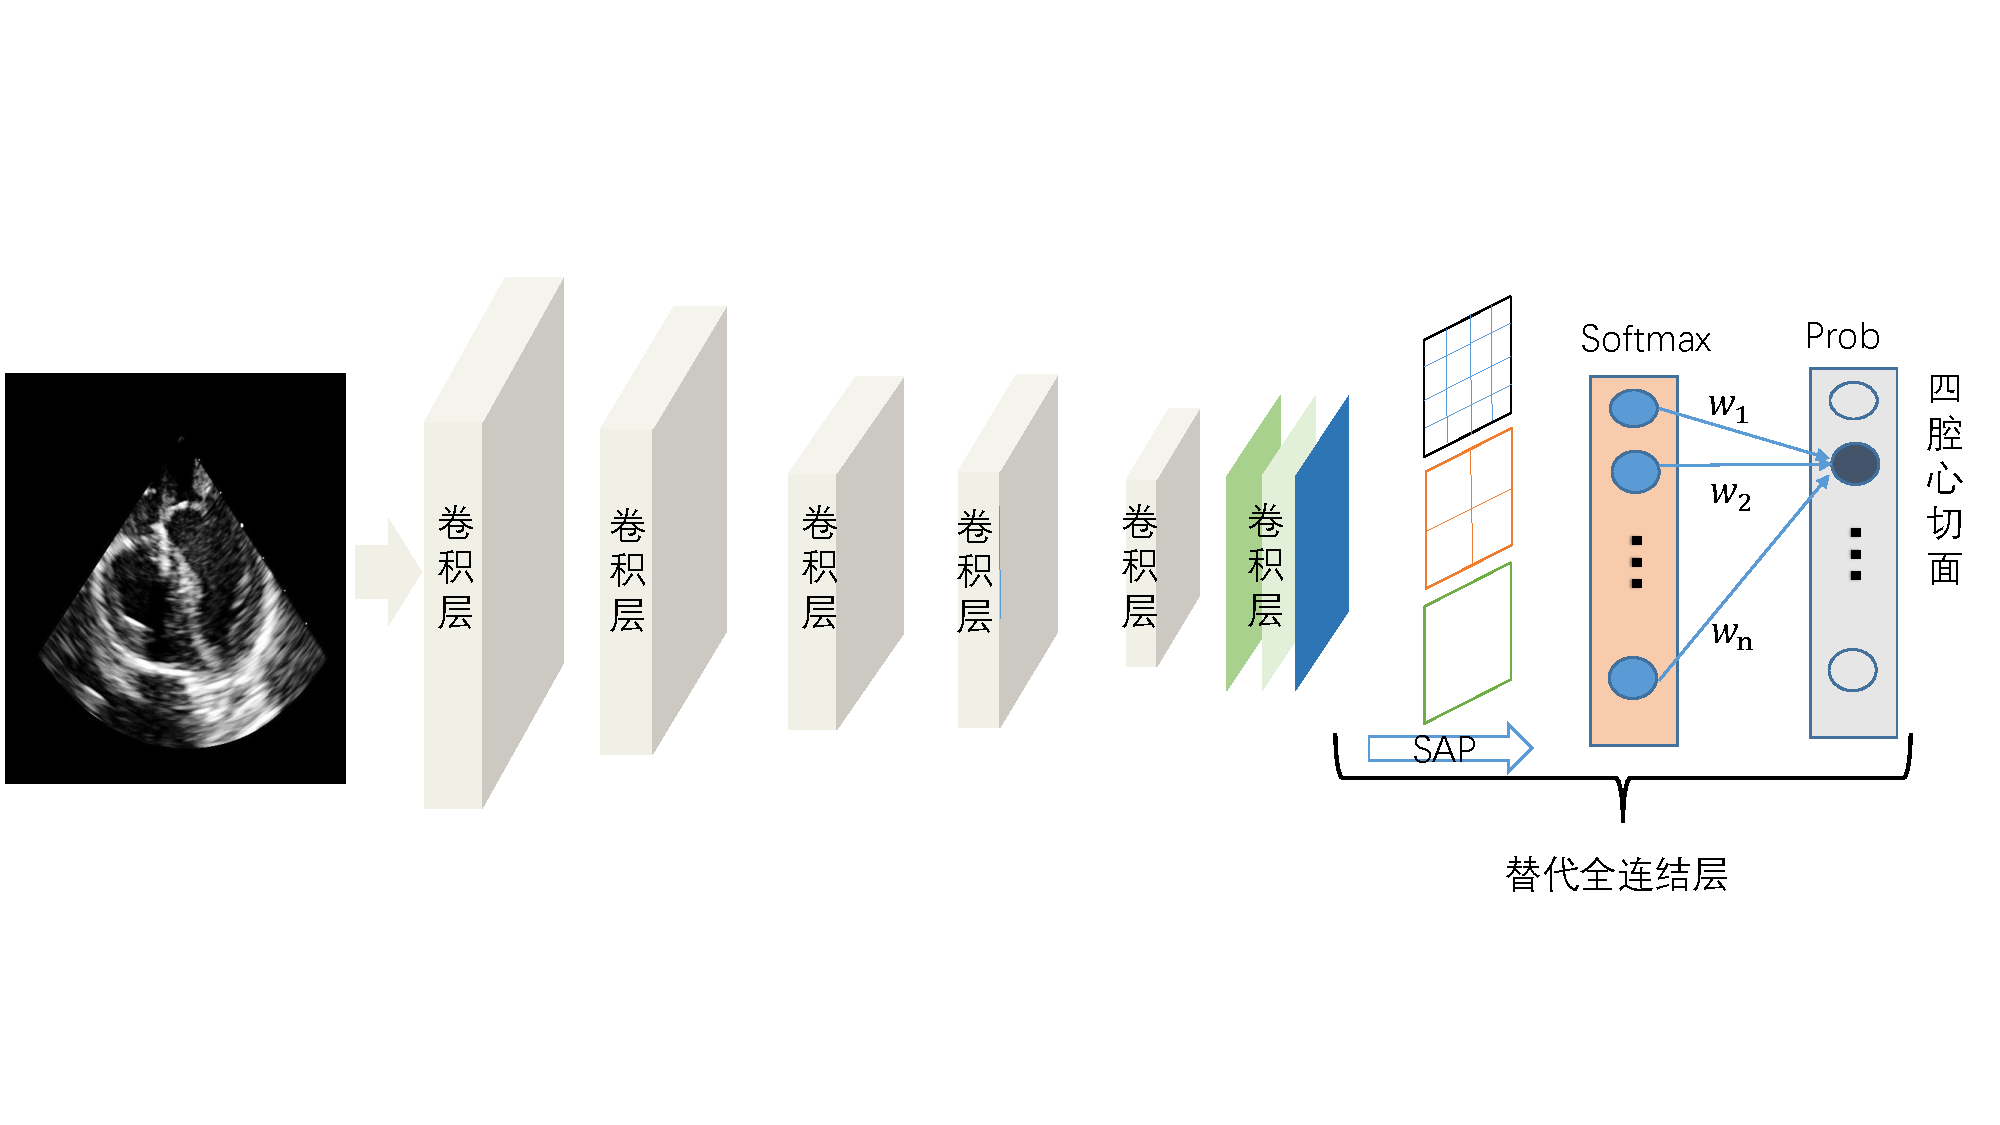
\includegraphics[trim = 30mm 0mm 30mm 0mm, clip, width=0.45\textwidth]{ch03_02}
    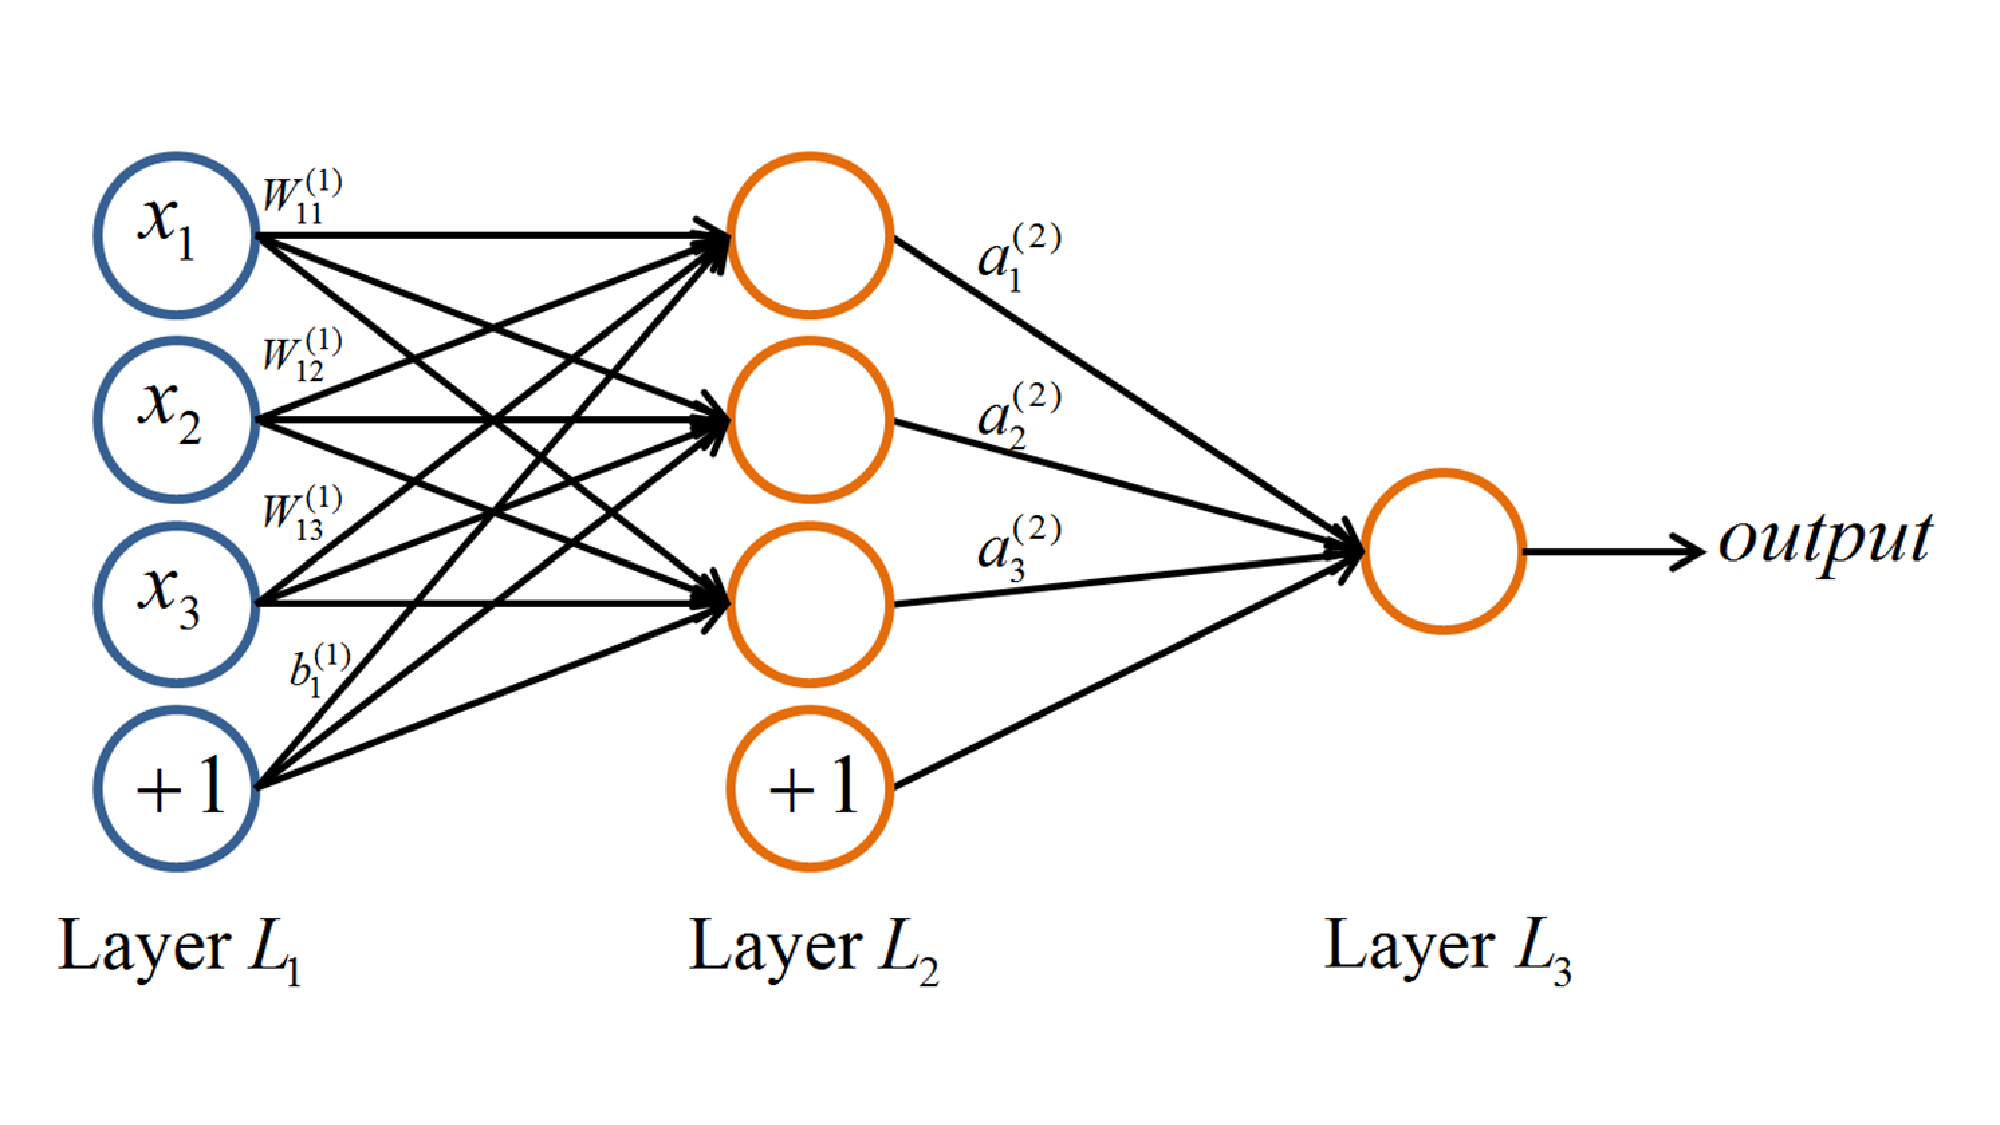
\includegraphics[width=0.9\textwidth]{ch02_01}
    \caption{前馈神经网络(也称为多层感知器)结构示例示意图}
    \label{fig:ch02_01}
\end{figure}

由于神经网络的非线性导致大多数代价函数都变得非凸,需使用迭代的基于梯度的优化,基于极大似然估计的随机梯度下降方法是目前最常用优化的方法,它将参数$\Theta$拟合到训练集 $\mathcal{D}$。反向传播(back propagation)算法可以用来高效地计算复杂函数的梯度,随机梯度下降中一般使用批量数据的一小部分用于梯度更新,在实践中优化最大可能性等价于最小化负对数似然,它与训练数据和模型分布间的交叉熵等价:
\begin{equation}
 \arg \min_{\Theta} - \sum^{N}_{n = 1} \log\big[ P(y_{n}| {\bf x}_{n}; \Theta) \big].
\end{equation}
其通常不直接优化我们感兴趣的目标,例如ROC曲线下的面积或用于分割的常用评估度量(例如Dice系数),该损失也称为交叉熵代价损失,。

长期以来,深度神经网络(Deep Neural Network,DNN)随着层数加深,优化函数越来越容易陷入局部最优解导致梯度弥散问题难以有效训练。从2006年开始才重新受到欢迎\citep{Hinton2006a},指出两种流行的无监督网络结构:堆叠自动编码器和深度置信网络,可以以无监督的方式逐层训练(预训练)DNN。但这些技术相当复杂需要大量手动调参才能产生令人满意的效果。

目前,最流行的模型是以有监督的方式进行端对端训练,通过引入预处理和新的激活函数,极大地简化了训练过程。最流行的网络结构是卷积神经网络和递归神经网络。尽管递归神经网络越来越受欢迎,但CNN目前在(医学)图像分析中应用最广泛。以下各节将简要介绍这些方法,从最受欢迎的方法开始,并讨论它们在应用于医疗问题时的差异和潜在的挑战。

\subsection{卷积神经网络}

卷积神经网络(CNN)是多层前馈神经网络的一种特例,是一种专门用来处理具有类似网格结构的数据的神经网络。,例如时间序列数据(可以认为是在时间轴上有规律地采样形成的一维网格)和图像数据(可以看作是二维的像素网格)。较普通神经网络引入了感受野、卷积核滤波器组、卷积层、池化层等概念,其隐藏层的神经元设计成跟上一层神经元局部稀疏连接,并利用参数共享来减少模型复杂度。针对图像这种结构化数据,由不同卷积核来探测不同空间位置上的局部统计特征。通过堆叠多层的卷积结构,实现从低层到高层语义空间的抽象映射。
\begin{figure}[!htbp]
    \centering
    %trim option's parameter order: left bottom right top
    %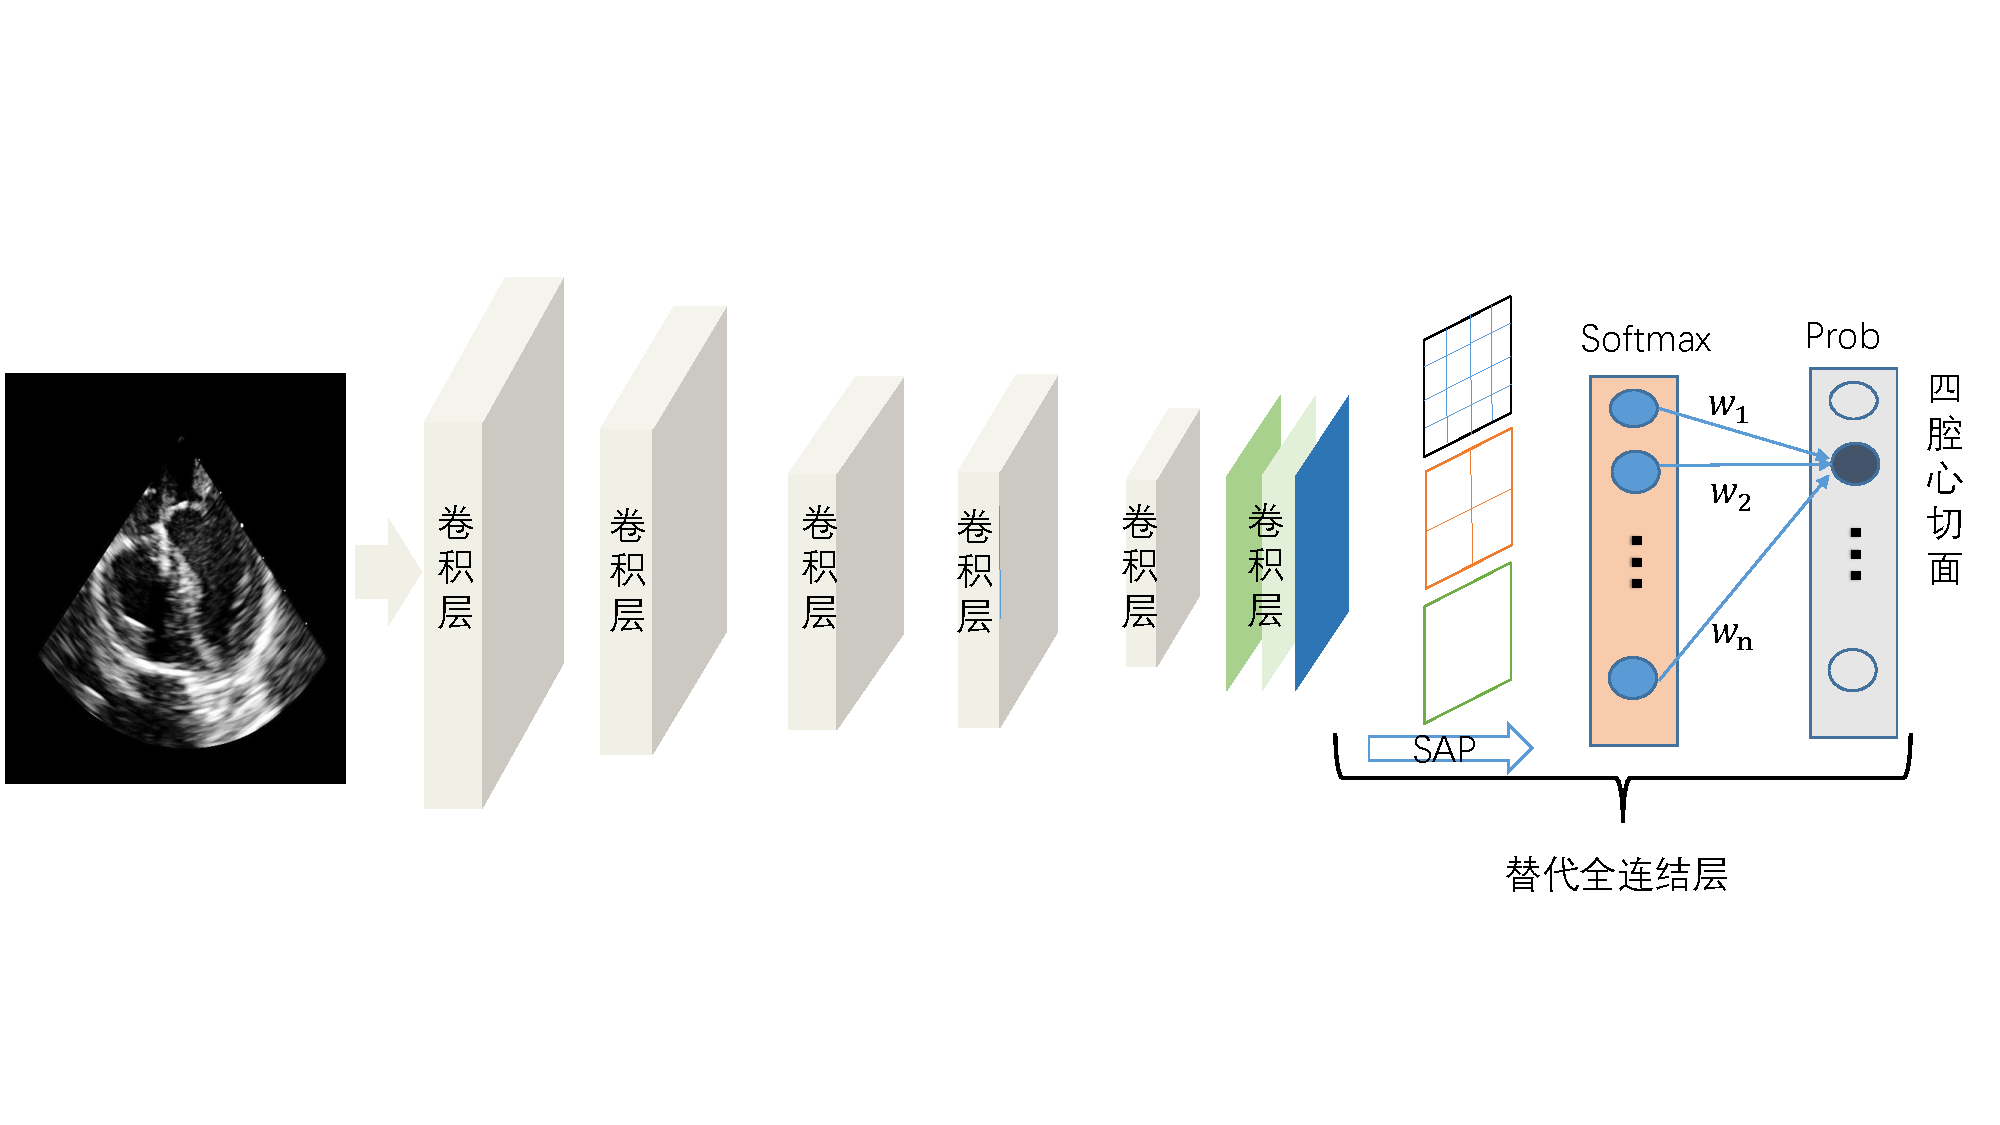
\includegraphics[trim = 30mm 0mm 30mm 0mm, clip, width=0.45\textwidth]{ch03_02}
    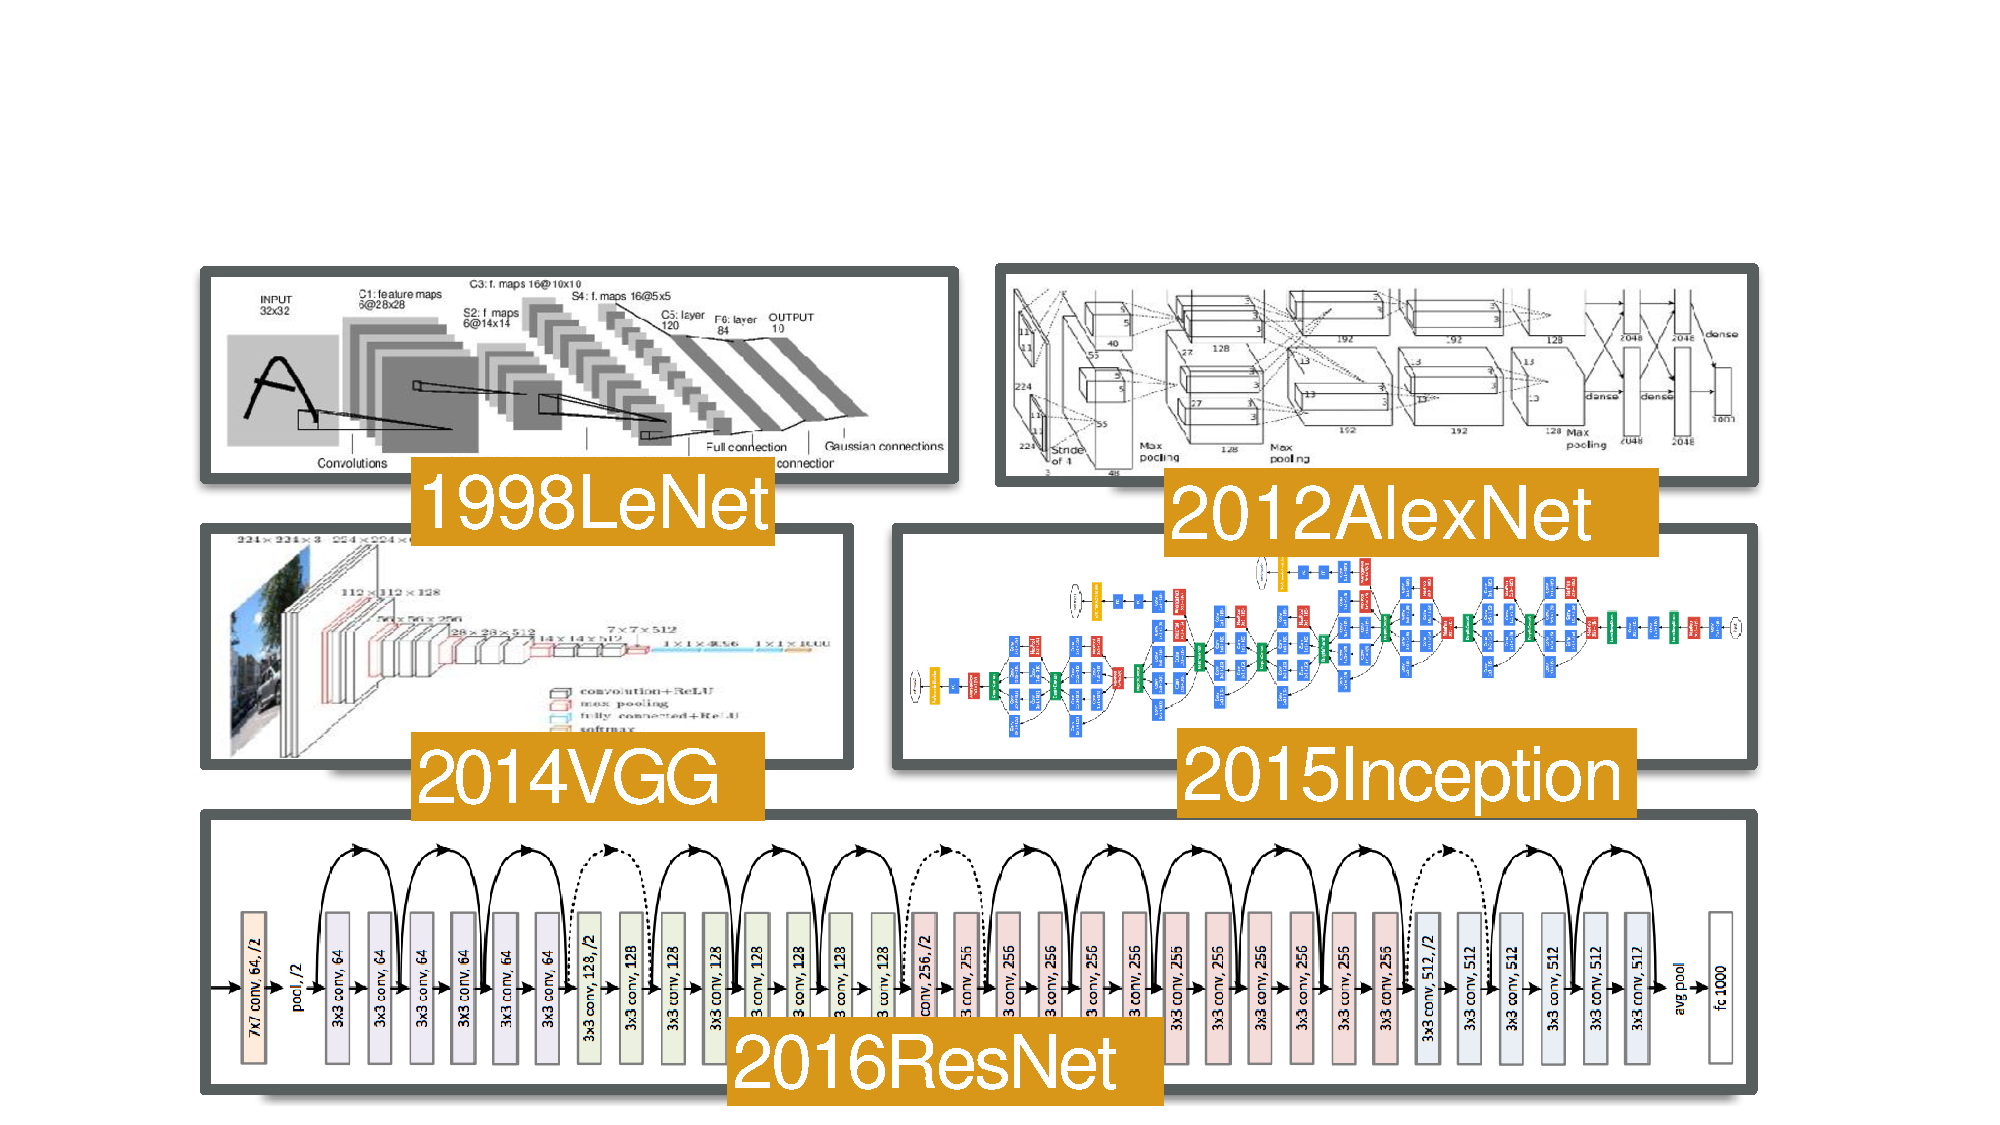
\includegraphics[width=0.9\textwidth]{ch02_02}
    \caption{经典深度网络结构示意图}
    \label{fig:ch02_02}
\end{figure}
MLP和CNN之间有两个关键的区别:首先,网络中的权重以网络对图像执行卷积操作的方式共享。这样,模型不需要为在图像中不同位置出现的同一对象分别检测单独的检测器,从而使网络在输入的平移时保持不变性。它还大大减少了需要学习的参数数量(即权重的数量不再取决于输入图像的大小)。图\ref{fig:ch02_02}中显示了LeNet-5\citep{Jarrett2009}的经典网络结构。

在每一层,输入图像与一组$K$卷积核进行卷积: $\mathcal{W} = \{ {\bf W}_{1}, {\bf W}_{2}, \ldots, {\bf W}_{K} \}$ 并添加偏差项$\mathcal{B} = \{b_{1}, \ldots, b_{K}\}$,每个生成一个新的特征映射(feature map)${\bf X}_{k}$。这些特征受到非线性变换$\sigma(\cdot)$的影响,并且对每个卷积层$l$重复相同的过程:
\begin{equation}
\label{eq::mapping_cnn}
 {\bf X}_{k}^{l} = \sigma\big( {\bf W}_{k}^{l -1} \ast {\bf X}^{l -1} + b_{k}^{l-1} \big).
\end{equation}

其次,在于CNN中的池化层(Pooling),其中邻域的像素值使用置换不变函数(通常是最大或平均运算)进行聚合。这会导致一定量的平移不变性,并再次减少网络中的参数数量。在网络的卷积层结束时,通常会添加全连接的层(即常规的神经网络层),其不再共享权重。类似于MLP,通过softmax函数概率归一化提供最后输出层中的激活值,并且使用方向传播优化极大似然损失对网络进行训练,从而产生类别概率分布。
\section{深度卷积神经网络}
鉴于CNN在医学图像分析中的流行,将详细介绍广泛使用的模型中最常见的网络结构及其差异,相关的方向的演进请参考图\ref{fig:ch02_04}。
\begin{figure}[!htbp]
    \centering
    %trim option's parameter order: left bottom right top
    %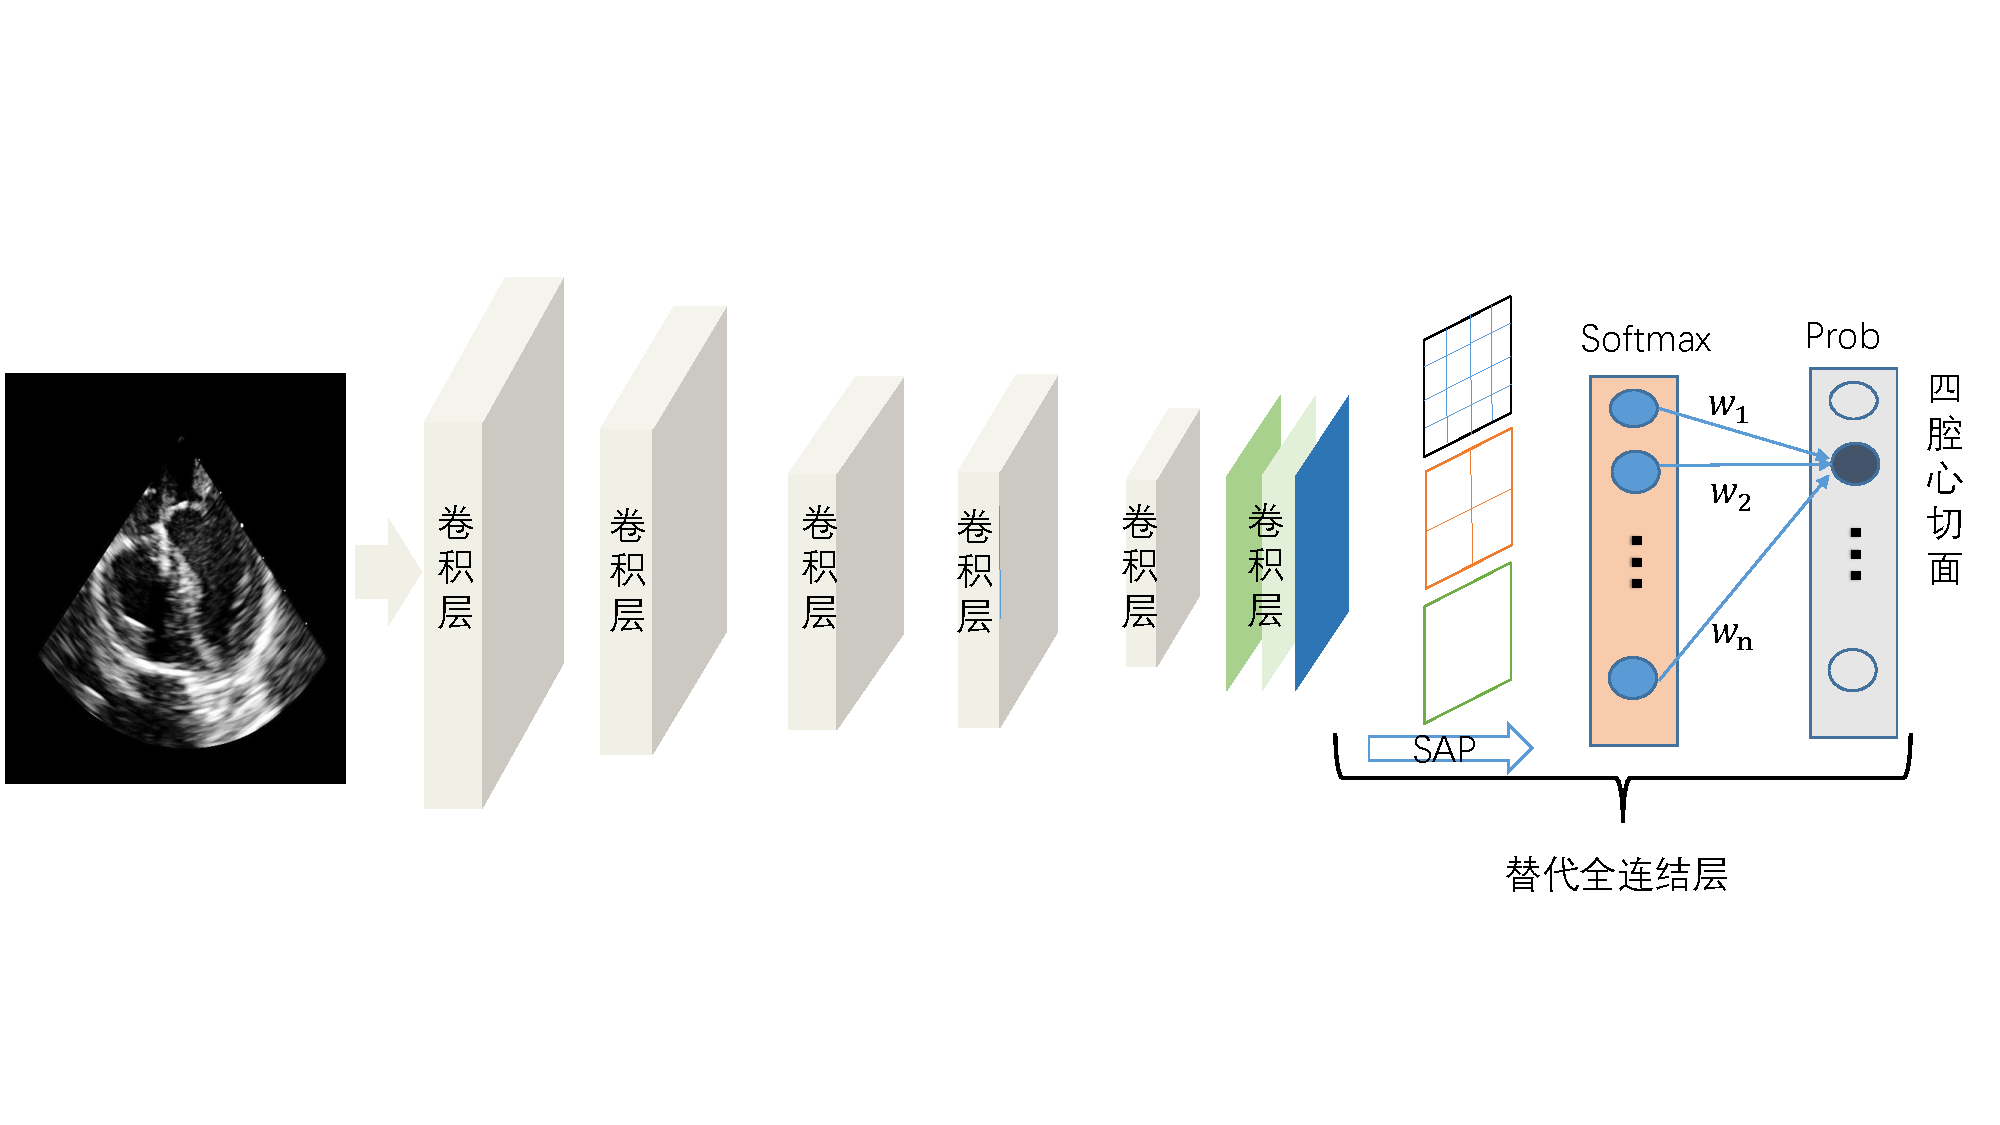
\includegraphics[trim = 30mm 0mm 30mm 0mm, clip, width=0.45\textwidth]{ch03_02}
    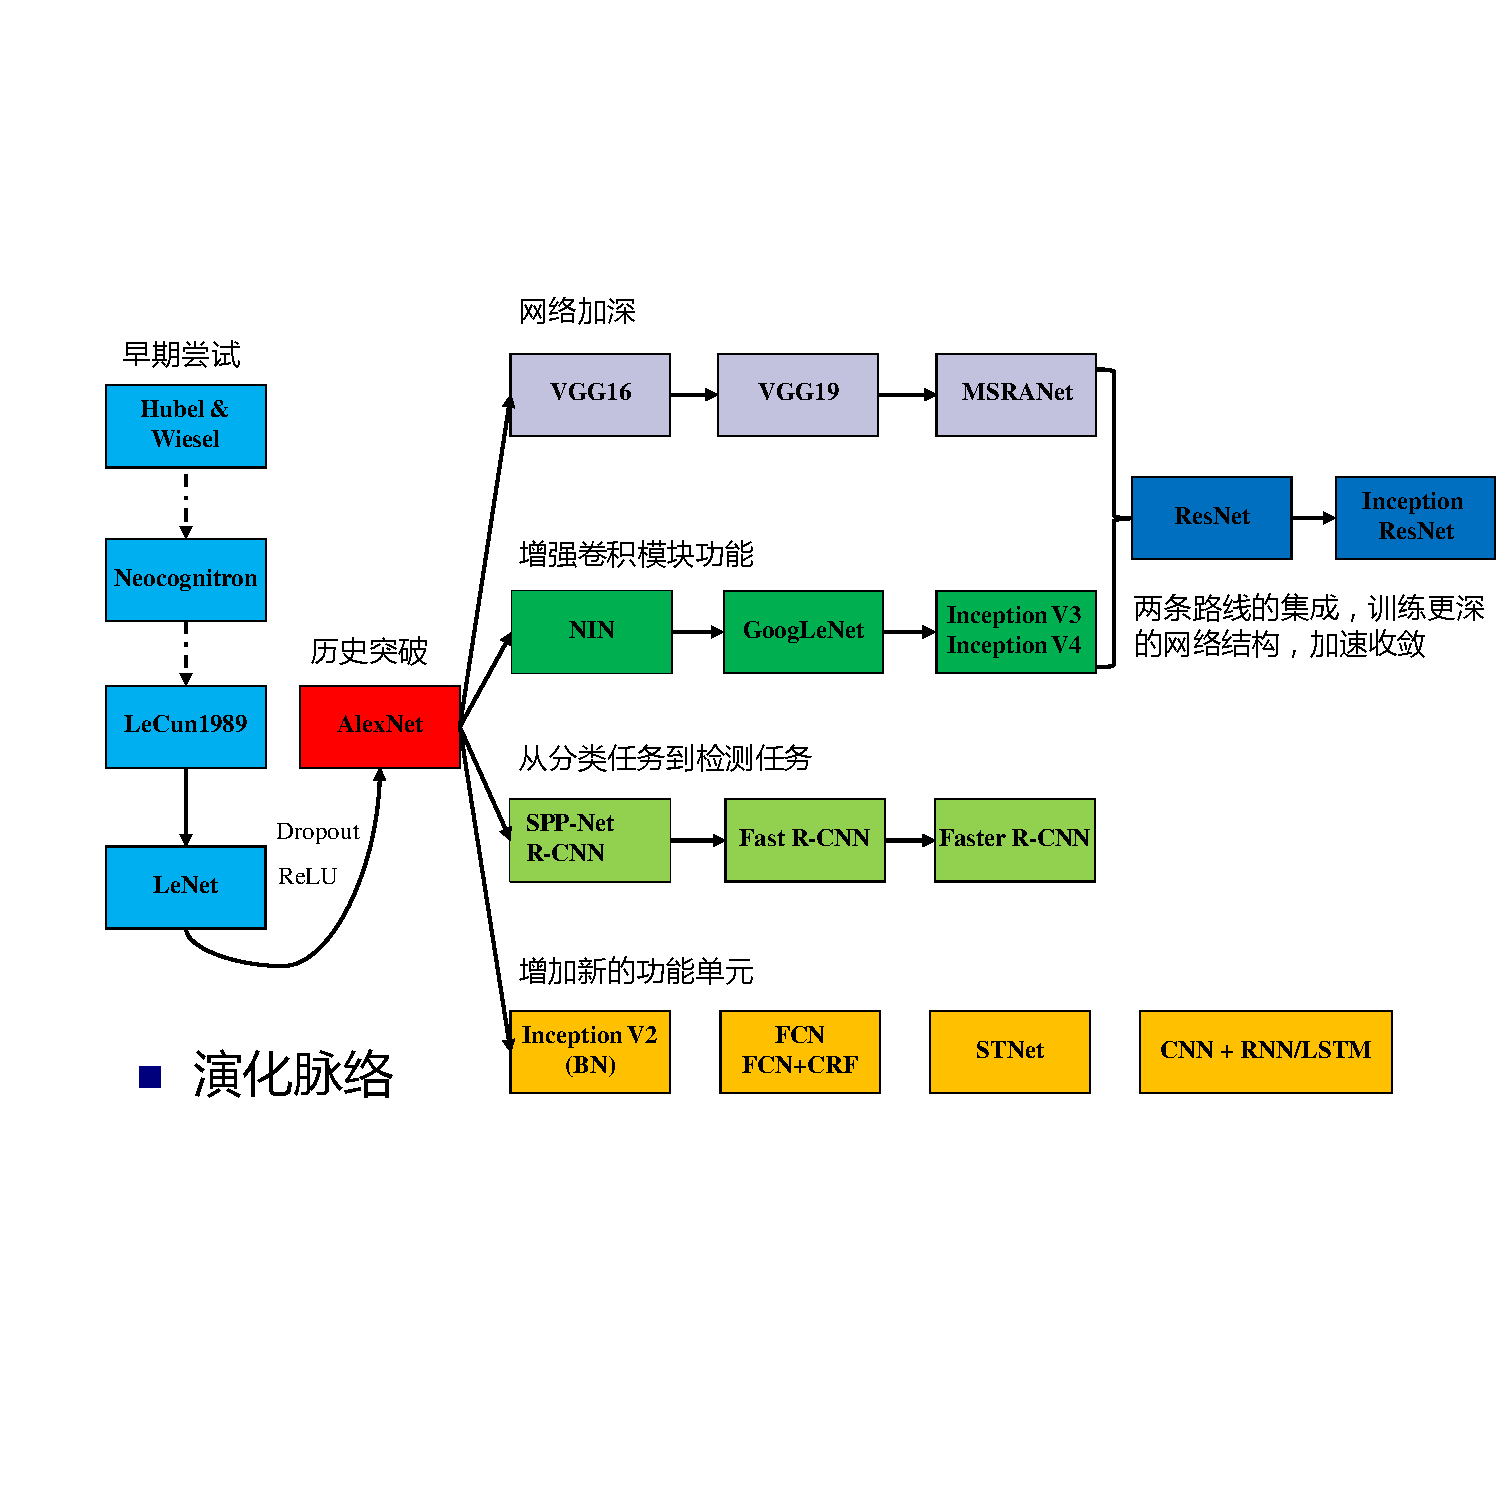
\includegraphics[height=60mm,width=0.9\textwidth]{ch02_04}
    \caption{深度卷积神经网络结构演进图}
    \label{fig:ch02_04}
\end{figure}
 
\subsection{通用分类框架}

深度CNN的典型结构AlexNet\cite{Krizhevsky2012}是在{\it LeNet}模型\citep{Jarrett2009}的基础上引入修正线性单元(Rectified Linear Units,ReLU)的激活函数和Dropout等技术\citep{Krizhevsky2012}进行的改进。模型的激活函数没有采用Sigmoid函数或双曲正切函数,而是选择ReLU函数,目的是引入更多非线性来加速训练收敛速度,解决多层网络反向传播中梯度弥散的问题。为了使得每层输入的分布更平稳,一般引入批量归一化层(Batch Normalization,BN)\cite{Ioffe2014Batch},采用最大池化层进行下采样,有时也把“卷积-激活-归一化-池化”统称为卷积层。最后需连接全连接层,全连接层就不再保存空间信息,是对低层特征的高层抽象,最终输出指定维度大小的向量,作为该图像的特征向量送入最终的分类器进行分类评估。
\begin{figure}[!htbp]
    \centering
    %trim option's parameter order: left bottom right top
    %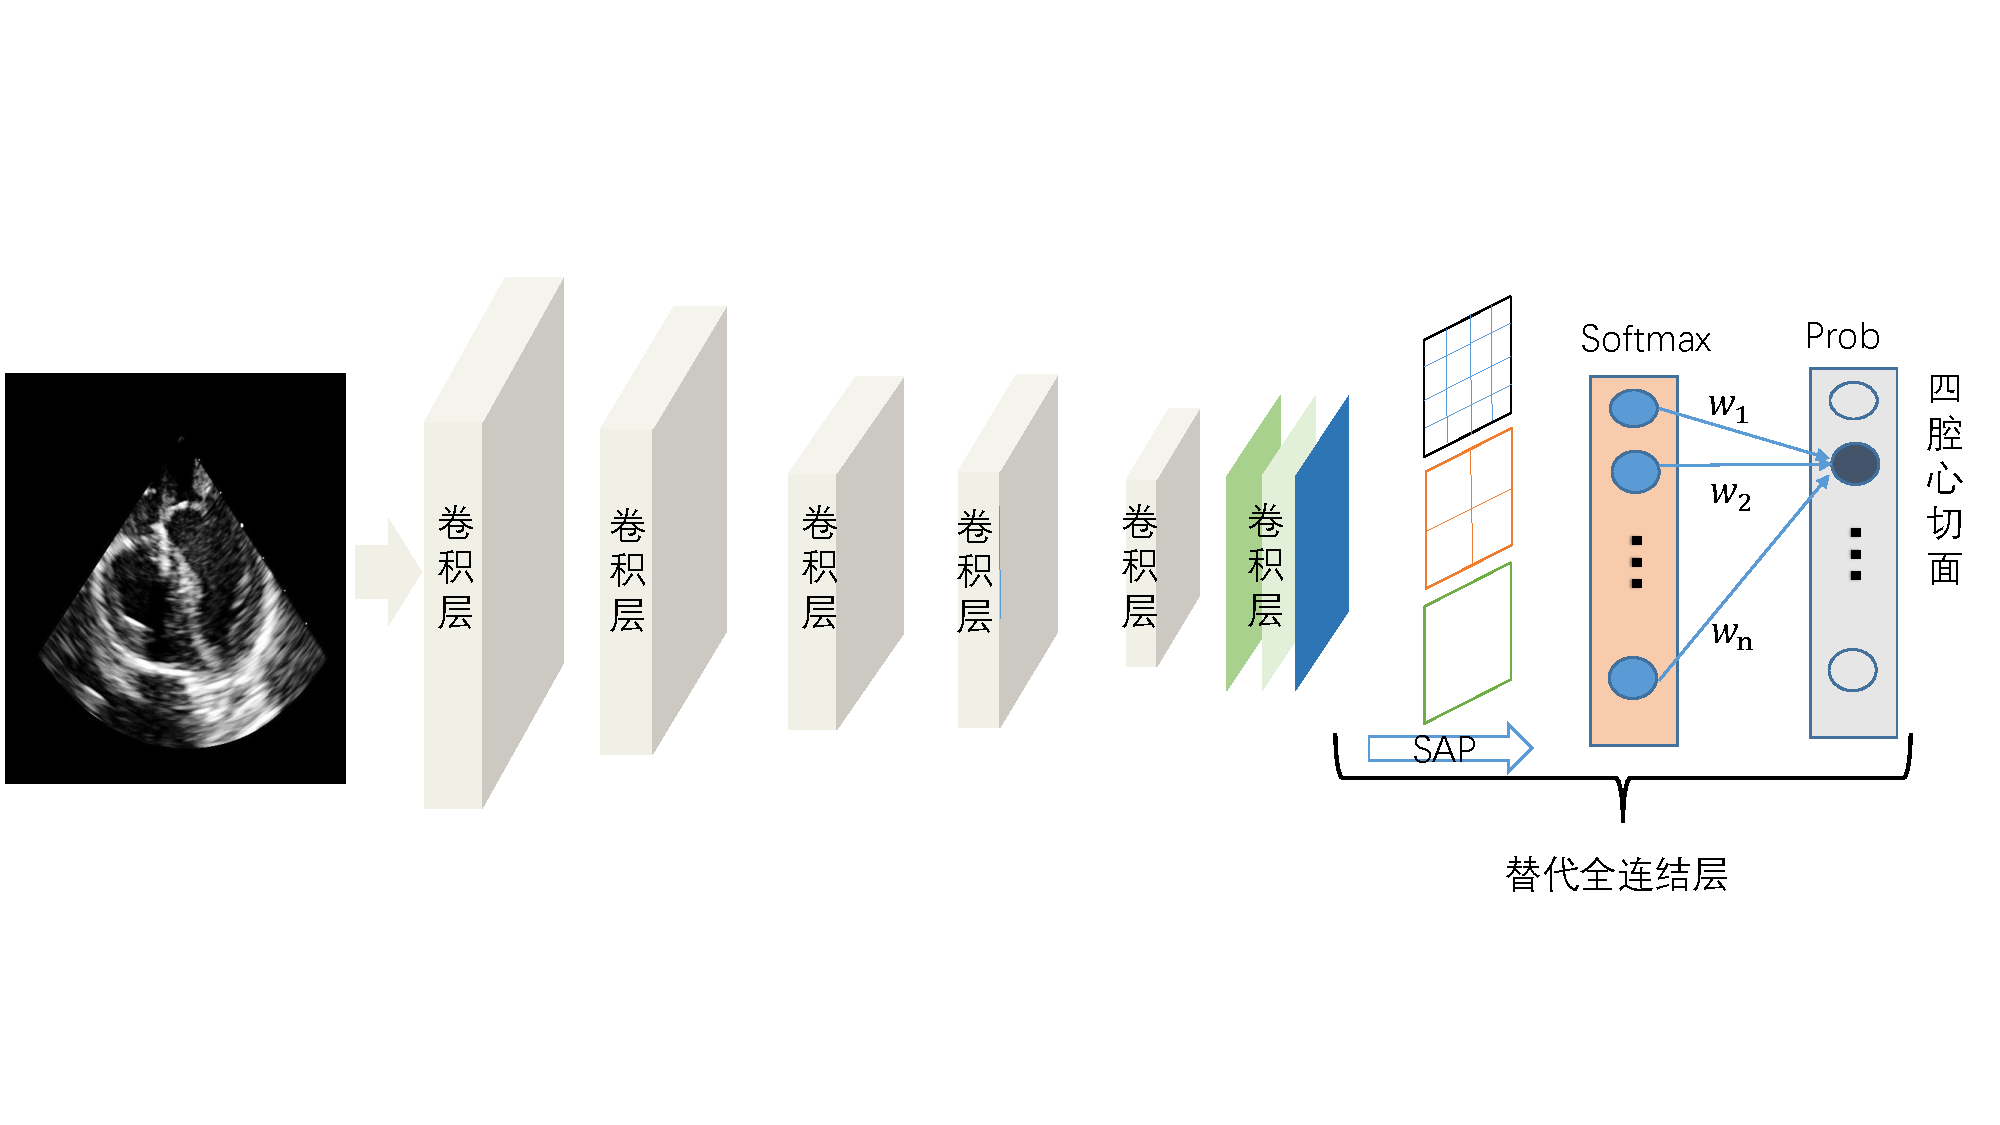
\includegraphics[trim = 30mm 0mm 30mm 0mm, clip, width=0.45\textwidth]{ch03_02}
    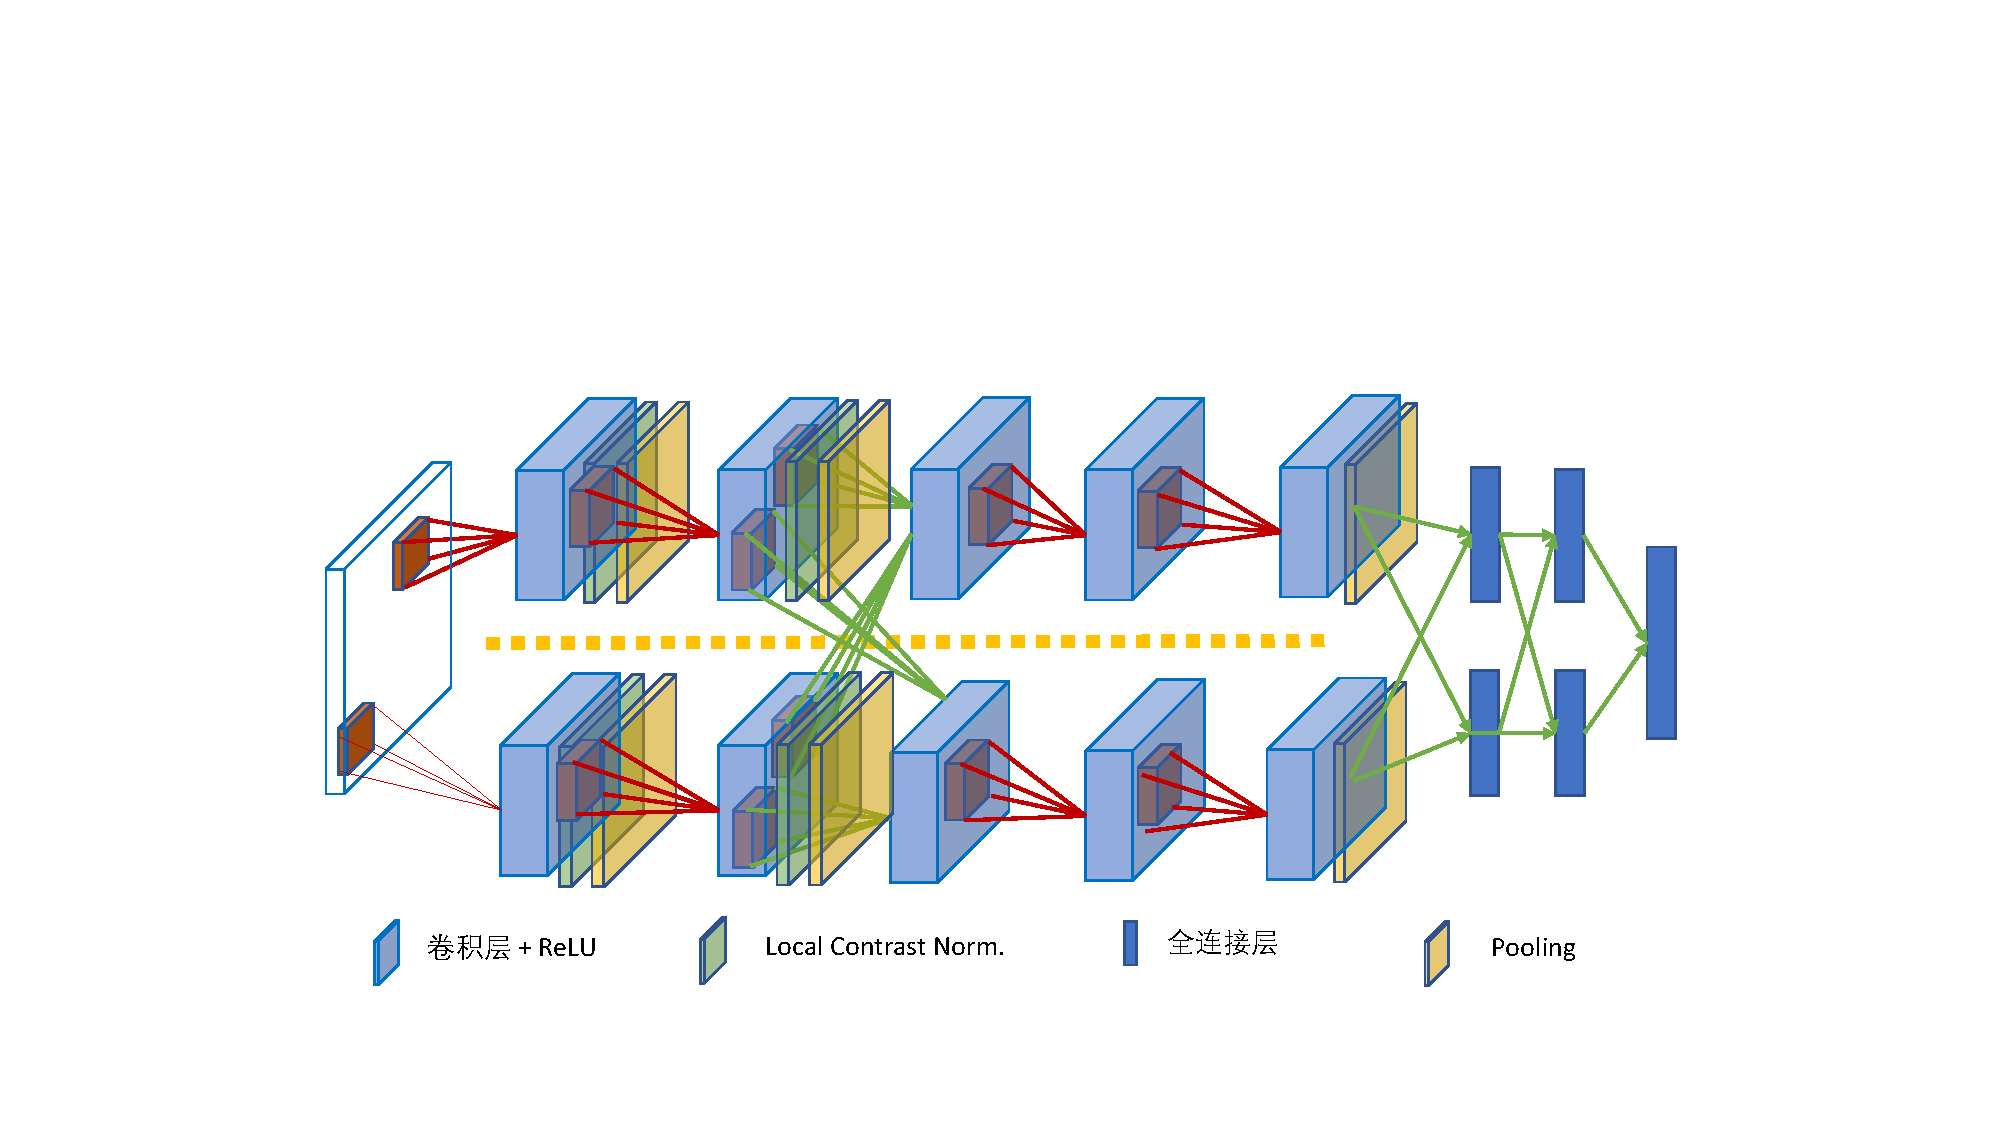
\includegraphics[width=0.9\textwidth]{ch02_03}
    \caption{AlexNet网络结构示意图\cite{Krizhevsky2012}}
    \label{fig:ch02_03}
\end{figure}
2012年以来新的网络结构不断涌现,模型更倾向于更深更复杂的结构。堆叠更小尺寸的卷积核,可以用较少的参数来表示类似的函数,这些更深的网络结构在推断时通常具有较低的内存占用量,这使得它们能够部署在诸如智能手机的移动计算设备上。{\it VGG}\citep{Simonyan2014a}是第一个探索更深层次的网络,网络的结构非常一致,从头到尾全部使用的是$3 \times 3$的卷积和$2\times 2$的池化层。Szegedy等\cite{Szegedy2015}提出了一个名为{\it GoogLeNet}的22层网络,在深层网络之上,引入了更复杂的构建模块,它使用使用密集连接结构用于估计稀疏CNN,也称为{\it Inception}模块\citep{Lin2013a},该模块使用一组不同大小的卷积$1 \times 1,3 \times 3,5 \times 5$的卷积取代了公式\eqref{eq::mapping_cnn};同时把顶部使用的全连接层替换成平均池化层,可以提高训练过程的效率,并再次减少参数的数量。{\it ResNet}网络结构\citep{he15}赢得了2015年的ImageNet挑战,其引入跳跃连接,残差块不是直接学习函数,而是仅学习残差,并因此预先调整每一层中学习接近同等函数映射,这样可以有效地训练更深的网络模型,可以认为{\it ResNet}是不同长度的网络的指数集合。

自2017年以来,ImageNet基准测试的性能已经饱和\cite{Deng2009ImageNet},虽然仍有很多分类识别的工作进行网络结构的设计,但很难评估性能的小幅增长是否真的归因于“更好”和更复杂的架构。这些模型所提供的较低内存占用空间的优势通常对于医疗应用来说并不重要。因此,{\it AlexNet}或其他简单模型(如{\it VGG、ResNet})仍然很受医学数据分析领域欢迎。

\subsection{多通路的卷积神经网络结构}
\label{sec:mc_architectures}
将深度学习技术应用于医疗领域的挑战通常在于将现有网络结构适应于例如不同输入格式,例如三维数据。在CNN早期应用于这样的体积数据时,通过将感兴趣体积(VOI)划分为切片,将全部3D卷积和由此产生的大量参数分开,所述切片作为不同的流馈送到网络。文献\citepns{Prasoon2013Deep}是第一个将这种方法用于膝关节软骨分割的。类似地,网络可以以多通道方式从3D空间中馈入多个角度的贴片\citep{Roth2014A},这些方法也被称为2.5D分类。

根据不同任务需要、不同融合方式可以得出多通路的网络结构,多个输入CNN网络的特征图可以在网络的任何处合并融合。如双通道架构\cite{Kamnitsas2017}可应用于多尺度图像分析;
在图像检测任务中,为了检测指定对象区域,上下文往往是一个重要的提示,增加上下文最直接的方法是将更大的区域块提供给网络,但这会显著增加网络的参数和内存需求量。因此除了提高分辨率获得局部信息之外,还可引入多通道多尺度网络结构\cite{Farabet2013Learning},一些医学应用也成功地使用该概念\citep{Kamnitsas2017,Moeskops2016Automatic,Song2015Accurate,Yang2016Cascade}。

\subsection{全卷积网络结构}
\label{sec:fully_arch}

分割和去躁是自然和医学图像分析中的一项常见任务,为了解决这个问题,CNN可分别对图像中的每个像素进行分类,需要在特定像素周围提取区域块。该“滑动窗口”方法的缺点是来自相邻像素的输入块具有巨大的重叠并且多次计算相同的卷积操作,卷积和点积都是线性算子,因此内积可以写成卷积,反之亦然,通过将全连接的层重写为卷积,CNN可以输入大于其被训练的图像尺寸的任意图像,并生成概率图。但由于池化合并图层,这可能导致输出的分辨率远远低于输入,反卷积\citep{Long2017Fully}是为防止这种分辨率下降而提出上采样方法之一,如图\ref{fig:ch02_05}。通过将结果拼接在一起,减去由于“有效”卷积而丢失的像素,可以获得最终输出的全分辨率完整输出。
\begin{figure}[!htbp]
    \centering
    \begin{subfigure}[b]{0.45\textwidth}
        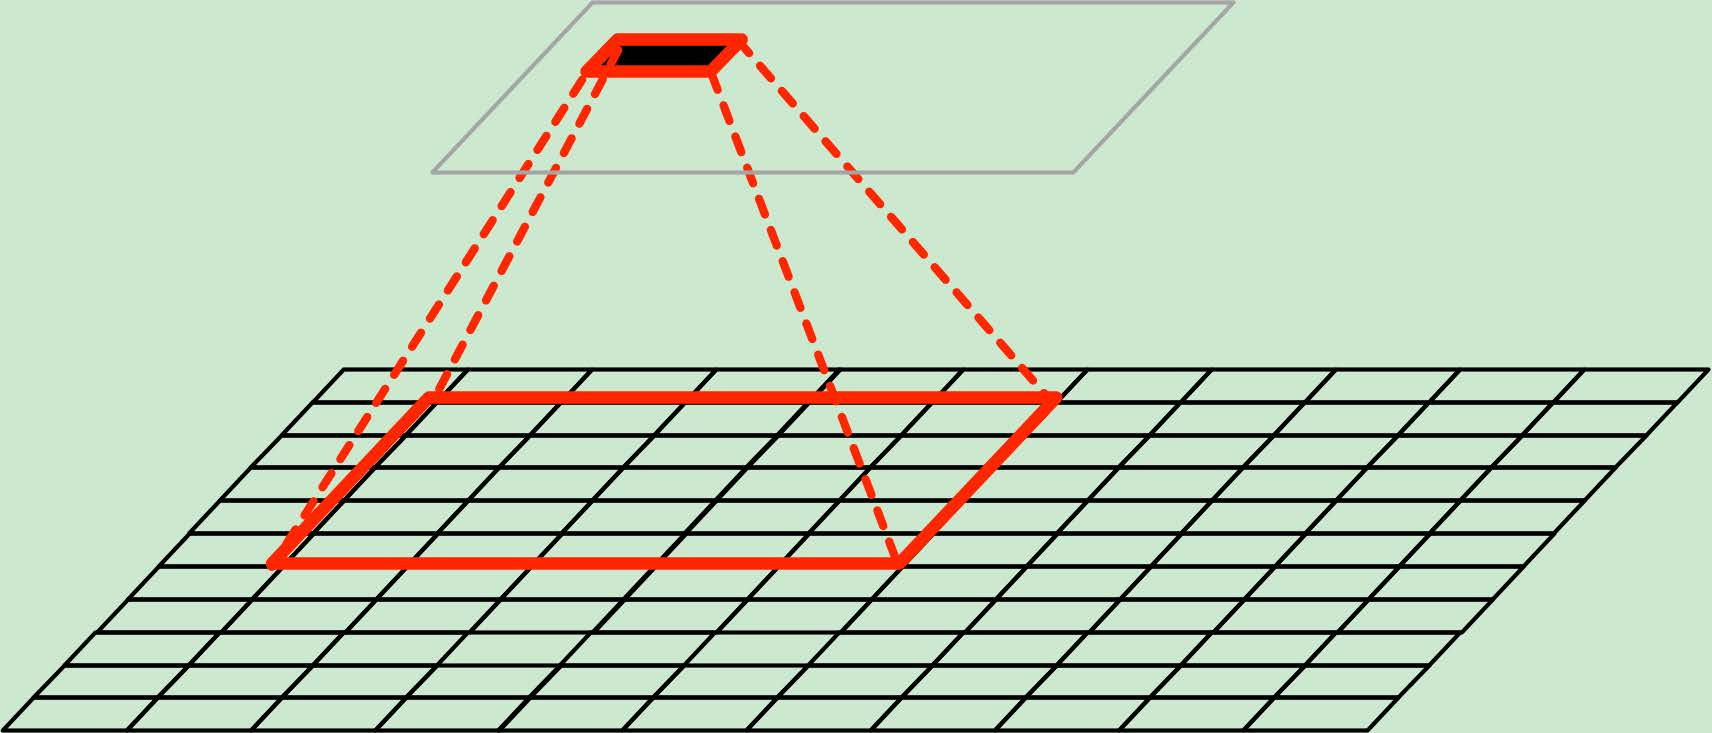
\includegraphics[height=30mm,width=\textwidth]{ch02_05_1}
        \caption{卷积}
        \label{fig:ch02_05_1}
    \end{subfigure}%
    % add desired spacing
    \begin{subfigure}[b]{0.45\textwidth}
        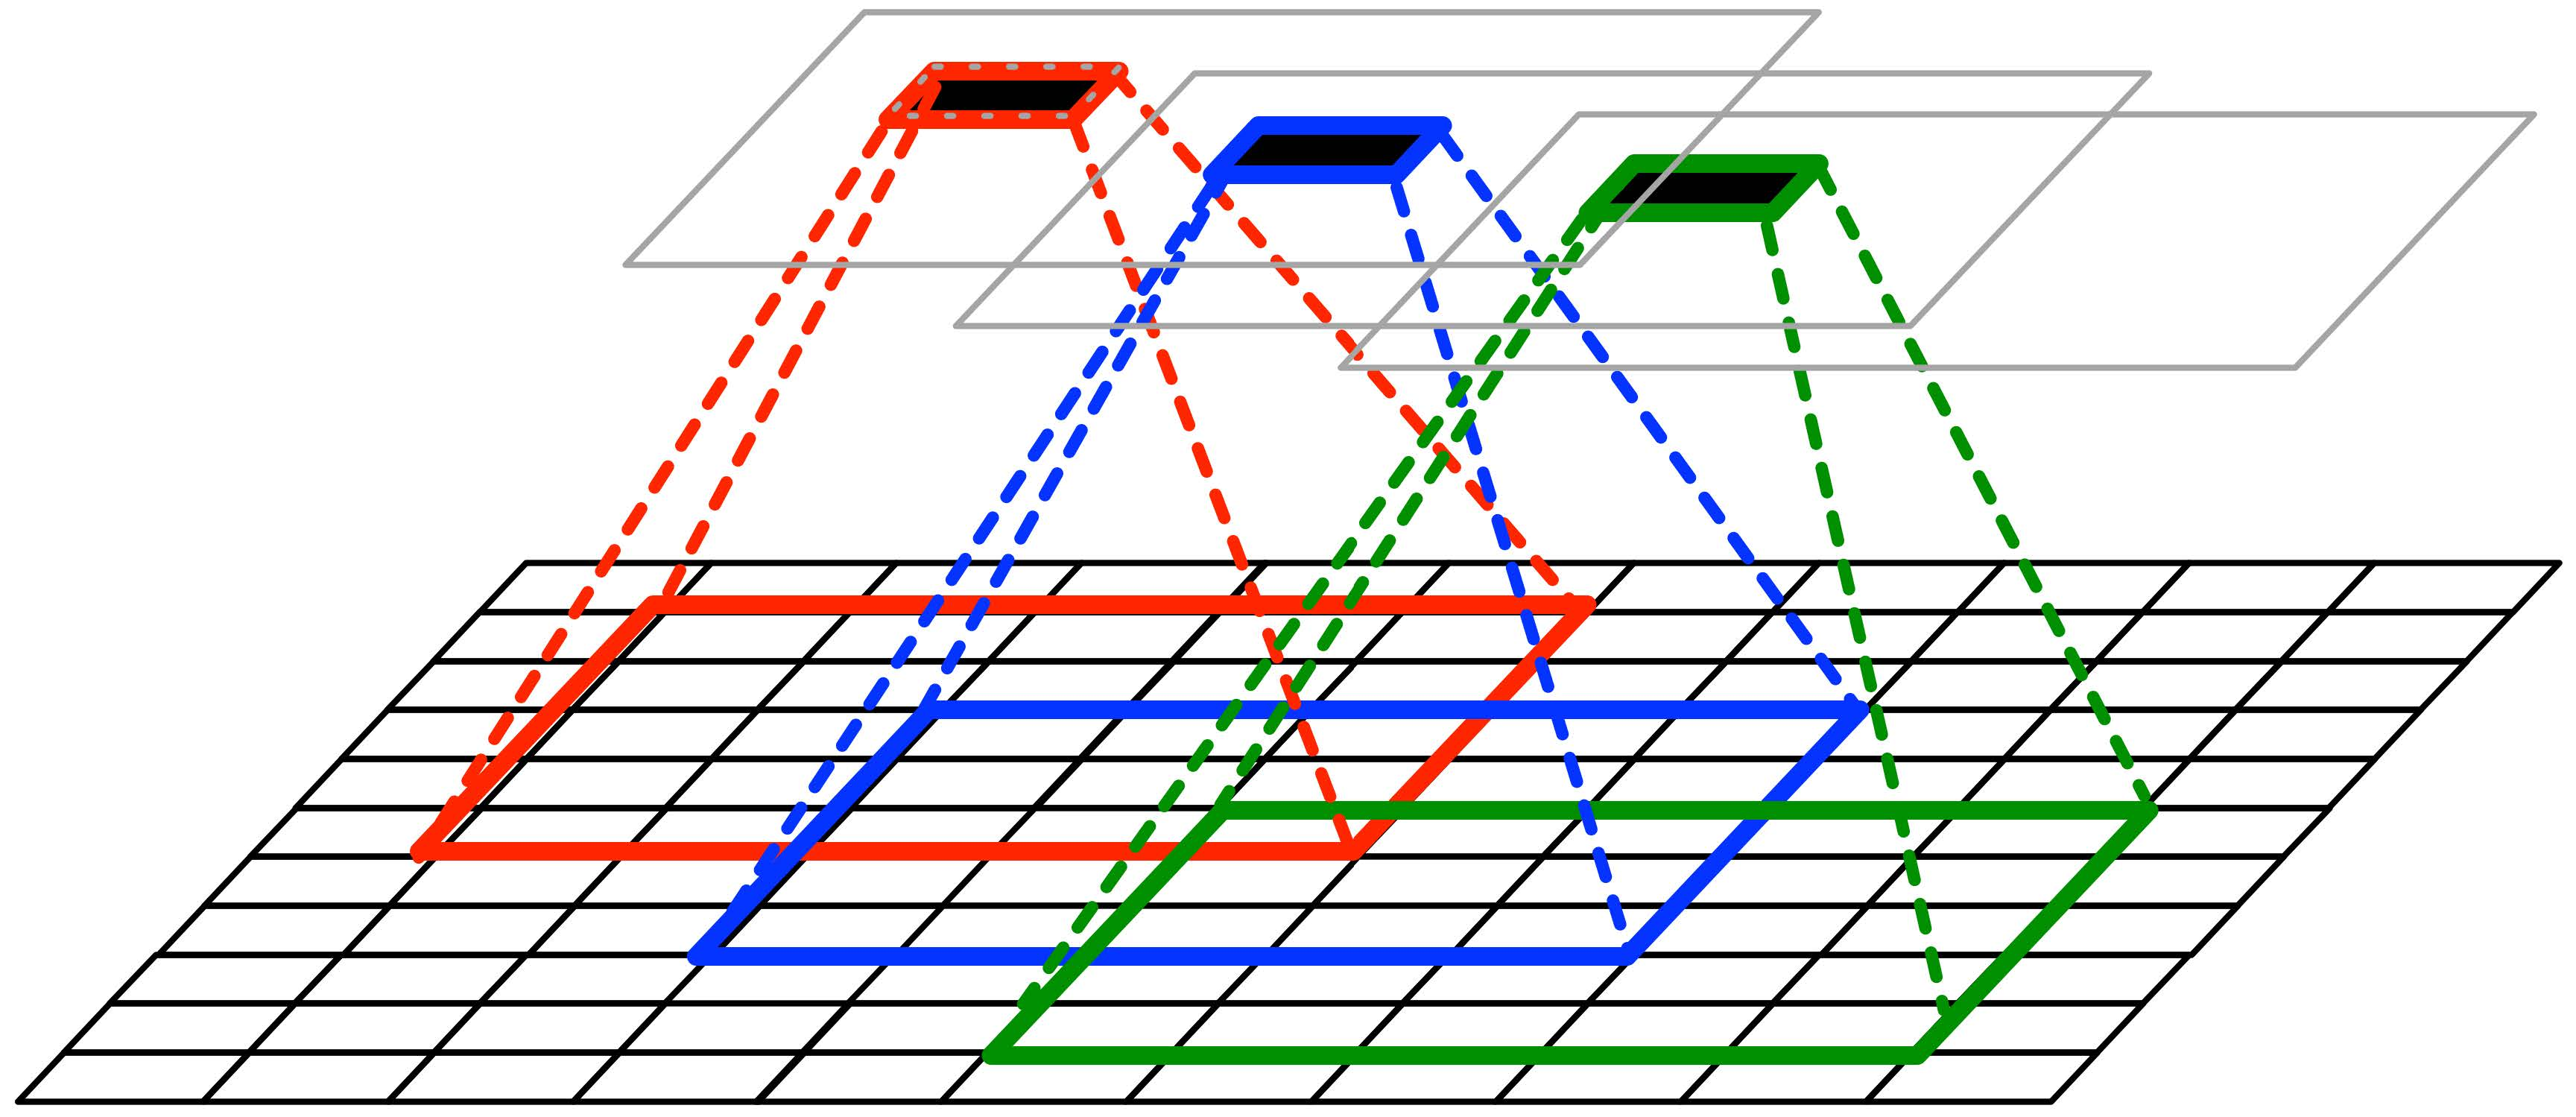
\includegraphics[height=30mm,width=\textwidth]{ch02_05_2}
        \caption{平铺卷积}
        \label{fig:ch02_05_02}
    \end{subfigure}
    % add desired spacing
    \begin{subfigure}[b]{0.45\textwidth}
        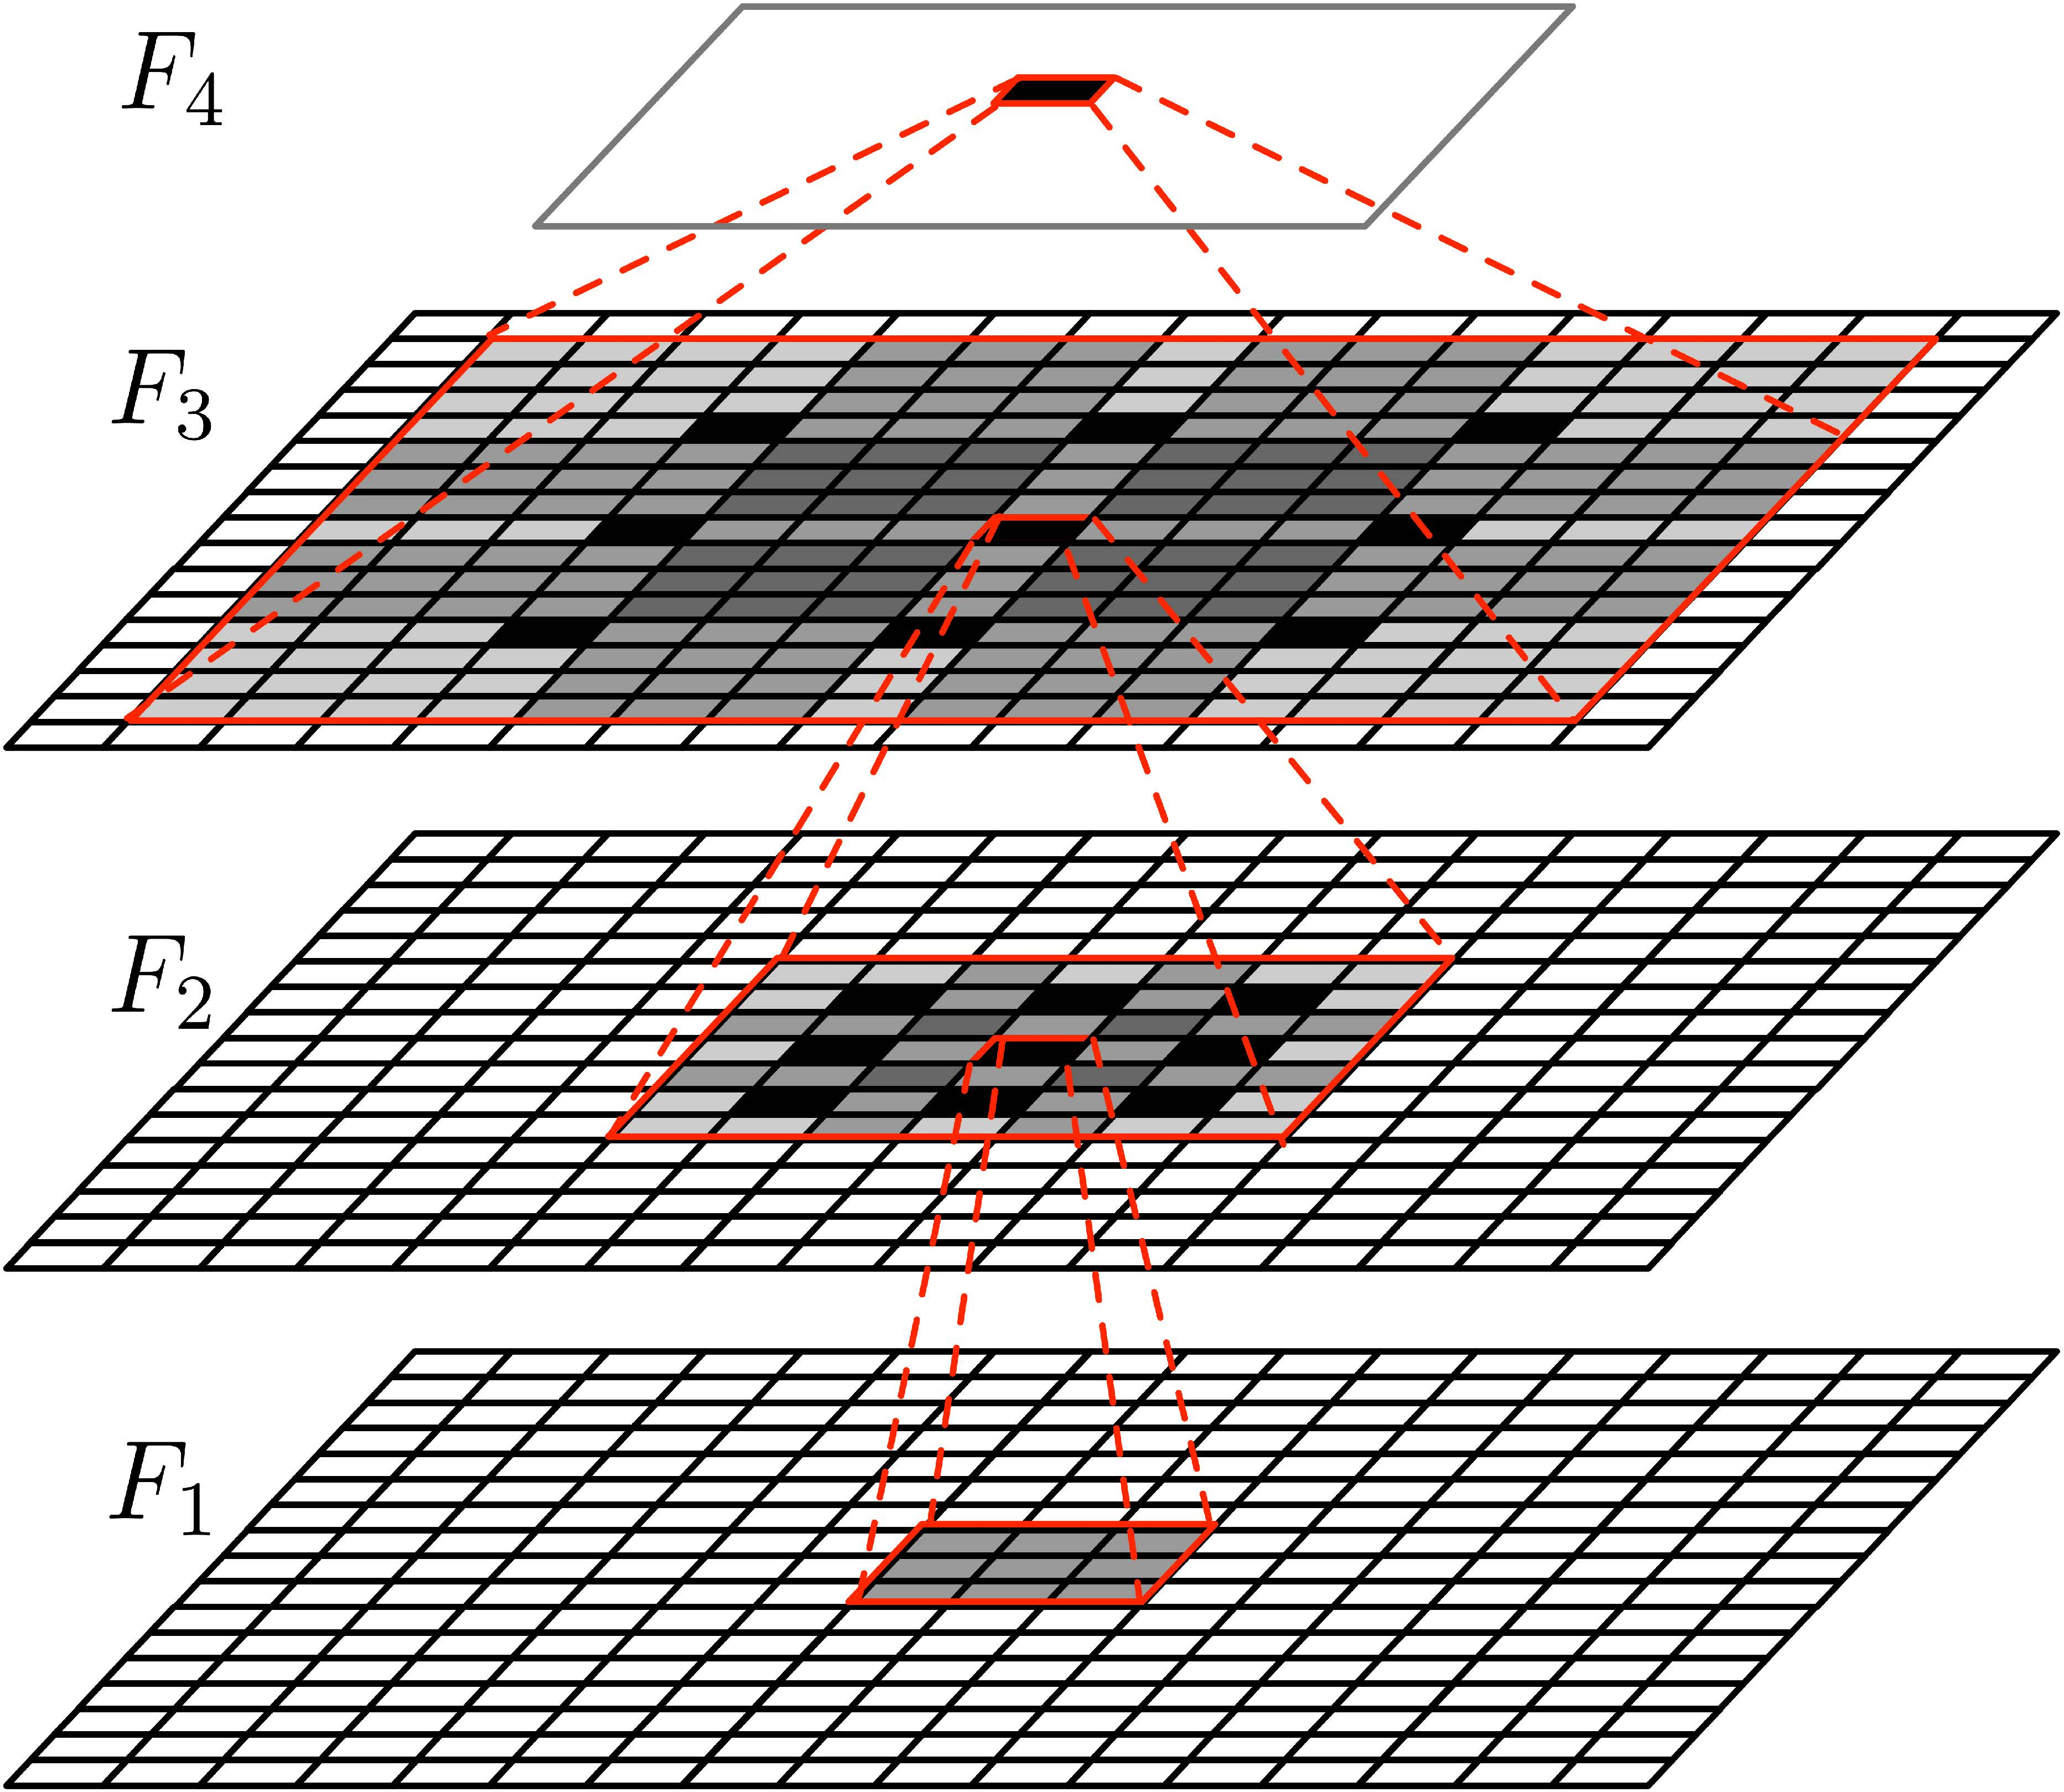
\includegraphics[height=30mm,width=\textwidth]{ch02_05_3}
        \caption{扩张(dilated)卷积}
        \label{fig:ch02_05_03}
    \end{subfigure}
    % add desired spacing
    \begin{subfigure}[b]{0.45\textwidth}
        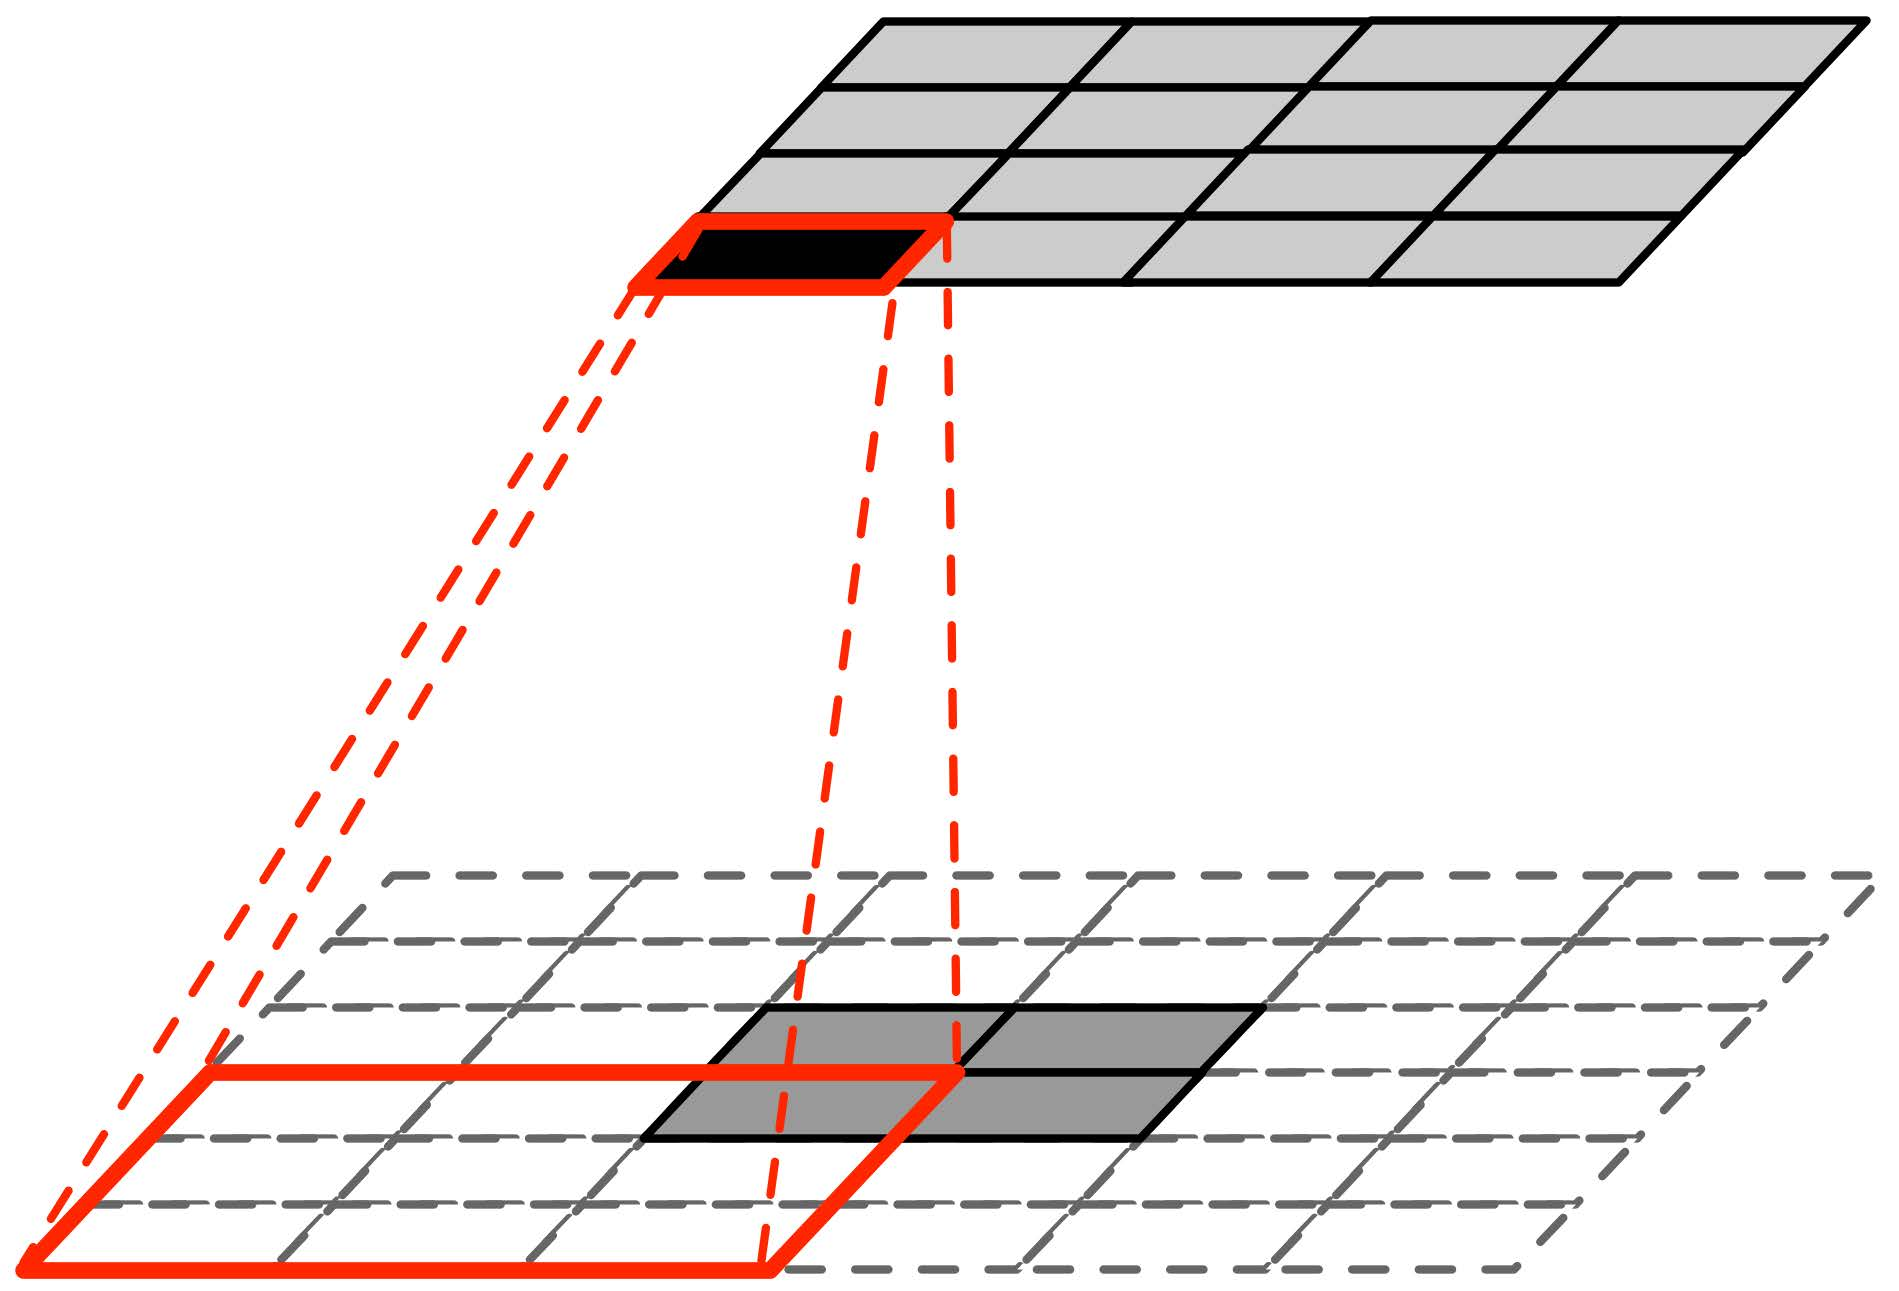
\includegraphics[height=30mm,width=\textwidth]{ch02_05_4}
        \caption{反卷积}
        \label{fig:ch02_05_04}
    \end{subfigure}
    \caption{卷积网络中的各种卷积操作图}
    \label{fig:ch02_05}
\end{figure}
将全卷积网络进一步改进提出U-net架构\cite{Ronneberger2015},其包含一个常规的全卷积结构,后面跟着一个上采样部分,其中反卷积用于增加图像大小,通过收缩编码-膨胀解码(Encoder-Decoder),将它与跳跃连接\citep{he15}相结合,提出Encoder-Decoder卷积层。3D数据也适用类似的方法,如用于体数据的V-Net结构,提出包含类似ResNet的残余块和随机丢失(Drop)层,损失函数也不是传统的交叉熵,而是直接最小化常用的分割误差测量损失\cite{Milletari2016}。

\section{循环神经网络}
\label{sec:rnns}

传统上RNN是为处理序列数据而开发的,可以看作是MLP的泛化,输入和输出的长度都不相同,这使得它们适用于诸如机器翻译、语音识别这样的任务,其中源语言和目标语言的句子是输入和输出。在分类设置中,模型学习了给出一个可变长度序列${\bf x}_{1}, {\bf x}_{2}, \ldots, {\bf x}_{T}$的类别$P(y | {\bf x}_{1}, {\bf x}_{2}, \ldots, {\bf x}_{T}; \Theta)$,而不是一个输入向量${\bf x}$。

普通的RNN在$t$时刻维持一个隐式或隐藏状态${\bf h} $,它是从其输入${\bf x}_{t}$和前一状态${\bf h}_{t-1}$:
\begin{equation}
 {\bf h}_{t} = \sigma({\bf W}{\bf x}_{t} + {\bf R}{\bf h}_{t - 1} + {\bf b}),
\end{equation}

其中加权矩阵${\bf W}$和${\bf R}$是随时间共享的。对于分类,通常会添加一个或多个完全连接的层,然后添加softmax以将序列映射到类别概率: 
\begin{equation}
 P(y | {\bf x}_{1}, {\bf x}_{2}, \ldots, {\bf x}_{T}; \Theta) = \text{softmax}( {\bf h}_{T}; {\bf W}_{out}, {\bf b}_{out}).
\end{equation}

由于梯度需要通过时间从输出反向传播,因此RNN具有固有的深度(及时性),因此与常规深层神经网络一样遭受梯度弥散难以训练问题。为此已经设计几种专用单元来解决上下文依赖问题,最早和最流行的是长期短期记忆(Long Short-Term Memory,LSTM)单元\citep{Hochreiter1997Long},而门控复发单元(Gated Recurrent Unit,GRU)\citep{Cho2014Learning}是LSTM的最新简化版。

尽管最初提出是针对一维输入,但RNN越来越多地应用于图像,在自然图像中,“pixelRNN”被用作自回归模型,生成模型最终可以生成类似于训练集样本的新图像。对于医疗应用,它们已被用于分割问题,并且在各种竞赛挑战中得到令人鼓舞的结果\citep{Stollenga2015Parallel}。

\section{无监督深度学习}
\subsection{自编码器}
自编码器(Auto-encoders,AE)是简单神经网络的一种,通过一个隐藏层${\bf h}$来产生编码(code)${\bf x}'$近似表示输入${\bf x}$。重建其隐藏层${\bf W}_{h, x'}$ 和相应的偏差$b_{h, x'}$,它们由权重矩阵和输入到隐藏状态和${\bf W}_{x, h}$的偏置$b_{x, h}$来控制。非线性函数用于计算隐藏激活: 
\begin{equation}
\label{eq::ae_projection}
 {\bf h} = \sigma({\bf W}_{x, h} {\bf x} + {\bf b}_{x, h}).
\end{equation}
此外,隐藏层$|{\bf h}|$的维度小于$|{\bf x}|$。这样,数据被投影到表示输入中的主要潜在结构的较低维子空间上。如果隐藏层的大小与输入大小相同,并且不再添加非线性,则模型将简单地学习标识函数,正则化或稀疏性约束可以用来增强发现过程。

去噪自动编码器\citep{Vincent2010Stacked}是另一种防止模型学习微不足道解决方案的解决方案。这里模型被训练来重构来自噪声损坏版本(通常是盐和胡椒噪声)的输入。SAE(或深度AE)通过将自动编码器层放置在彼此之上而形成。相关医疗应用中,自动编码器层经常被(“贪婪算法”)单独训练,然后使用监督训练对整个网络进行微调以进行预测。

\subsection{受限波兹曼机和深度信念网络}
受限玻尔兹曼机(Restricted Boltzmann Machines,RBMs)\citep{Hinton2006a}是一种马尔可夫随机场,构成输入层或可见层${\bf x} = (x_{1}, x_{2}, \ldots, x_{N})$和一个带有潜在特征表示的隐藏层${\bf h} = (h_{1}, h_{2}, \ldots, h_{M})$。节点之间的连接是双向的,因此给定输入向量$\bf x$可以获得潜在特征表示$\bf h$,反之亦然。因此,RBM是一个生成模型,我们可以从中进行抽样并生成新的数据点。与物理系统类比,能量函数被定义为输入和隐藏单位的特定状态$({\bf x}, {\bf h})$:
\begin{equation}
 E({\bf x}, {\bf h}) = {\bf h}^{T}{\bf W}{\bf x} - {\bf c}^{T}{\bf x} - {\bf b}^{T}{\bf h},
\end{equation}
与 ${\bf c}$ and ${\bf b}$ 偏差条款。系统的“状态”的概率通过将能量传递给指数和正态化来定义:
\begin{equation}
 p({\bf x}, {\bf h}) = \frac{1}{Z} \exp\{ - E({\bf x}, {\bf h}) \}.
\end{equation}
计算分区函数 $Z$通常是棘手的。然而,以${\bf h}$为条件计算${\bf v}$形式的条件推断是可以处理的,并且会产生一个简单的公式:
\begin{equation}
 P(h_{j} | {\bf x}) = \frac{1}{ 1 + \exp\{ -b_{j} - {\bf W}_{j}{\bf x}\} }.
\end{equation}
由于网络是对称的,类似的表达式适用 $P(x_{i} | {\bf h})$.

DBNs \citep{Hinton2009Deep}实质上是AE层被RBM取代的堆叠多层AE。再次,以无人监督的方式进行单个层次的训练。通过向DBN顶层添加线性分类器并执行监督优化来执行最终的微调。
\subsection{变分自编码器和深度生成对抗网络}
最近,引入了两种新颖的无监督网络结构:变分自动编码器(VAE)\citep{Kingma2013Auto}和生成对抗网络(GAN)\citep{Goodfellow2014Generative}。因很难解决它们配分函数的数值而成为众所周知的难题,目前还没发现将这些方法应用于医学图像,但在自然图像中的应用还是值得期待的。

\section{深度学习相关技术}
在本节中,我们将从激活函数,损失函数,正则化和优化四个方面描述CNN的主要改进方向。
\subsection{激活函数}
\label{Activationfunctions}
合适选择激活函数能显着提高了CNN对于某个任务的性能。在本节中,我们将介绍CNN中几种激活函数。

\subsubsection{ReLU}

ReLU激活函数定义如下:
\begin{equation}\label{eq:ReLU}
a_{i,j,k}=\max(0,z_{i,j,k})
\end{equation}
其中$ z_{i,j,k} $是位置$ (i,j) $第$k$个通道的输出,ReLU是一个分段饱和线性函数,它将负数部分修剪为零,并保留正数部分(参见\figurename {\ref{fig:ReLU}})。ReLU的取$ \max $操作的计算速度比sigmoid或tanh激活函数快得多,并且它还可以诱导隐藏单元的稀疏性并允许网络获得稀疏表示。
文献表明,甚至在没有预训练的情况下,使用ReLU可以有效地训练深度网络\cite{Krizhevsky2012}。
\subsubsection{带泄漏的ReLU}

ReLU单元的一个潜在缺点是只要单元不激活,它就具有零梯度。基于梯度的优化不会调整它们的权重,这可能会导致最初没有激活的单位以后永不会激活。此外,由于恒定的零梯度,它可能会减慢训练过程。为了缓解这个问题,Mass等\cite{Maas2013}引入了带泄漏(Leaky)的ReLU(LReLU),其定义如下:
\begin{equation}\label{eq:LReLU}
    a_{i,j,k}=\max(0,z_{i,j,k})+\lambda\min(0,z_{i,j,k})
\end{equation}
其中$ \lambda $是$(0,1)$范围内的预定义参数。与ReLU相比, LReLU使得具有负向值而不是将其映射到常量零点,这使得当单元不活动时允许一个小的非零梯度。
\subsubsection{带参数的整流线性单元}

不同于在LReLU中使用预定义的参数,而是在等式(\ref{eq:PReLU})中给出带参数的整流线性单元(PReLU),其自适应学习参数以提高准确性。在数学上,PReLU函数定义为
\begin{equation}\label{eq:PReLU}
    a_{i,j,k}=\max(0,z_{i,j,k})+\lambda_k\min(0,z_{i,j,k})
\end{equation}
其中$ \lambda_k $是第$ k $通道的待学习参数。由于PReLU仅引入极少量的额外参数,例如,额外的参数数量与整个网络的通道数量相同,因此不会出现过度拟合的额外风险,额外的计算成本可以忽略不计。它也可以通过反向传播与其他参数同时训练。

\subsubsection{随机整流线性单元}\label{RReLU_comp}
LReLU的另一个变体是随机整流线性单元(RReLU)\cite{xu2015ecirical},在RReLU中负值部分的参数从均匀分布中随机抽样,然后在测试中使用固定值(参见\figurename {\ref{fig:RReLU}})。形式上RReLU函数定义如下:
\begin{equation}\label{eq:RReLU}
    a^{(n)}_{i,j,k}=\max(0,z^{(n)}_{i,j,k})+\lambda^{(n)}_k\min(0,z^{(n)}_{i,j,k})
\end{equation}
其中$ z^{(n)}_{i,j,k}$是位置$ (i,j) $上第$n$个样例的第$k$个通道的输出, $ \lambda^{(n)}_k $表示其对应的采样参数,$a^{(n)}_{i,j,k}$表示其相应的输出。由于其随机性,它可以减少过度拟合。Xu等\cite{xu2015ecirical}也对标准图像分类任务中的ReLU,LReLU,PReLU和RReLU进行评估,并得出结论:在整流激活单元中加入一个非零斜率用于负值部分,可以持续改善性能。

\subsubsection{指数线性修正单元}
Clevert等\cite{Clevert2015}引入了指数线性单元(Exponential Linear Unit,ELU),它可以更快地学习深度神经网络,并提高分类精度。像ReLU、LReLU、PReLU和RRELU一样,ELU通过将正部分设置为线性变换来避免渐消梯度问题。与同样具有负值部分的LReLU,PReLU和RReLU相比,ELU使用饱和度函数作为对噪声更鲁棒的负值部分。ELU的函数定义如下:
\begin{equation}\label{eq:ELU}
    a_{i,j,k}=\max(0,z_{i,j,k})+\min(0,\lambda(e^{z_{i,j,k}}-1))
\end{equation}
其中$ \lambda $是用于控制ELU为负输入饱和的值的预定义参数。
\begin{figure}
	\centering
	\begin{tabular}[c]{ccc}
		\begin{subfigure}[c]{0.25\textwidth}
			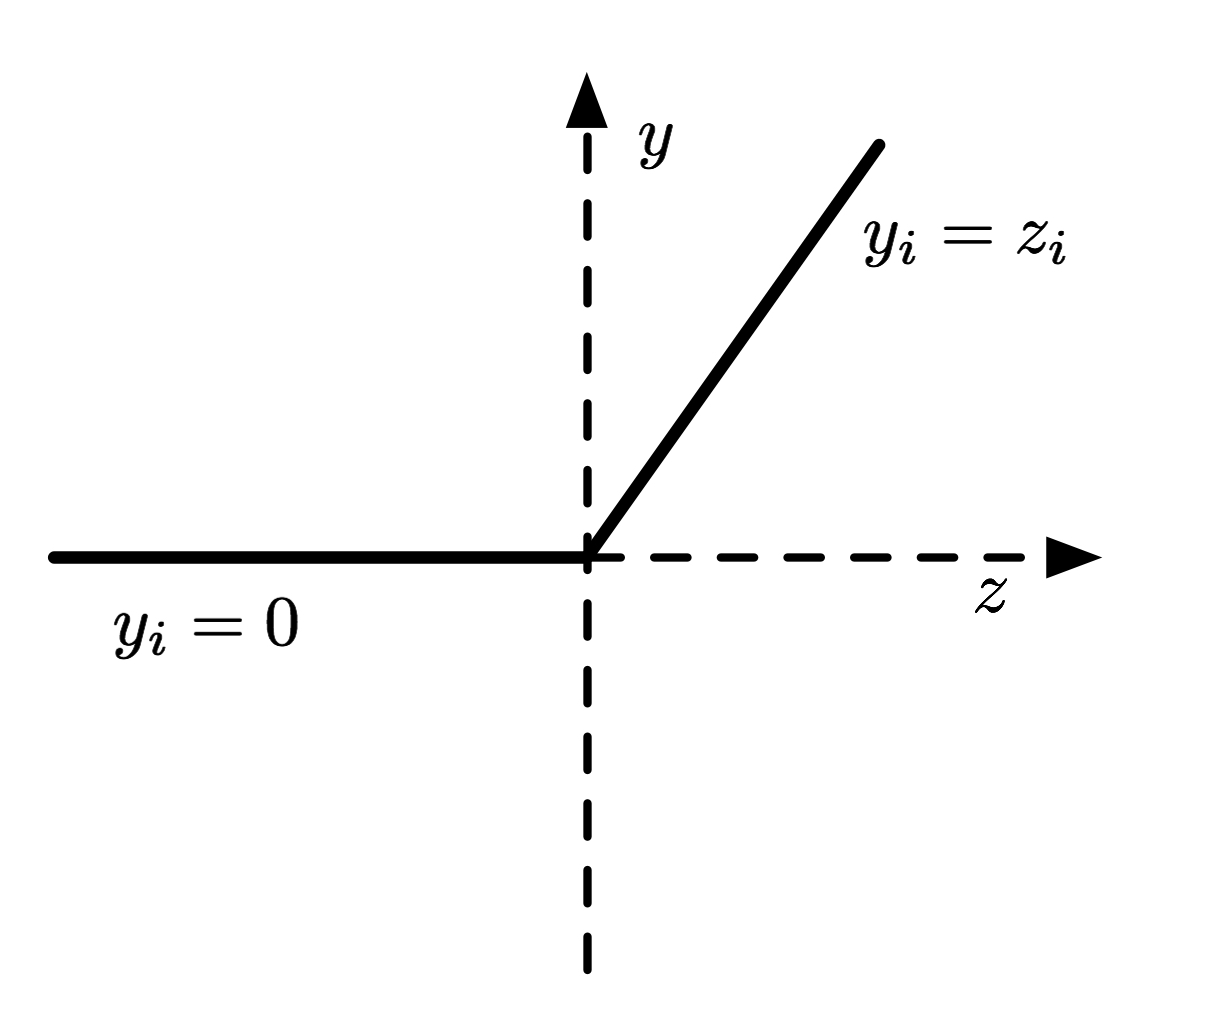
\includegraphics[height=30mm,width=\textwidth]{ch02_06_01.jpg}
			\caption{ReLU}
			\label{fig:ReLU}
		\end{subfigure}&
		\begin{subfigure}[c]{0.25\textwidth}
			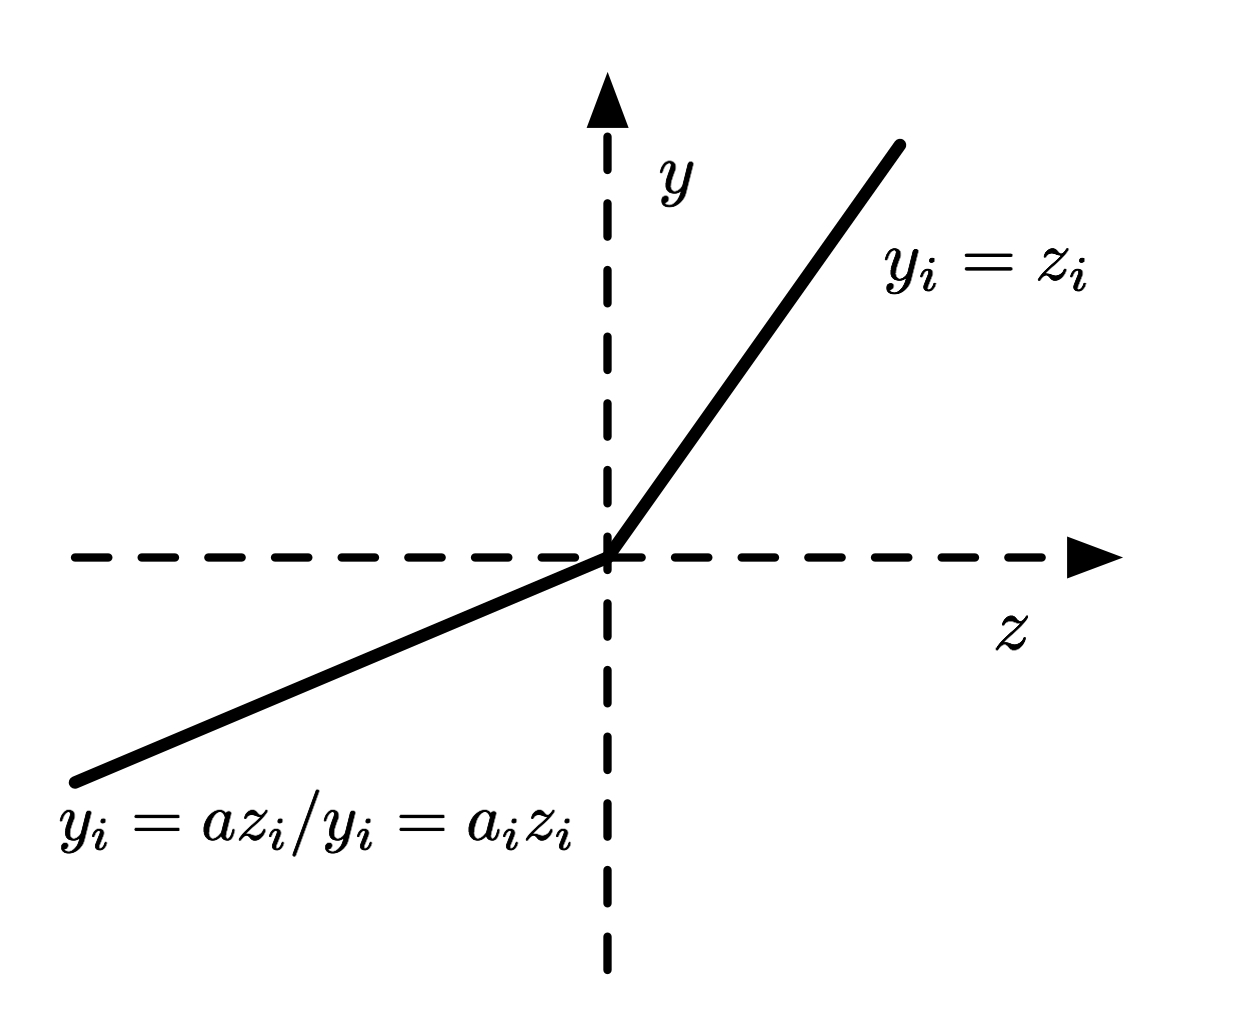
\includegraphics[height=30mm,width=\textwidth]{ch02_06_02.jpg}
			\caption{LReLU/PReLU}
			\label{fig:PReLU}
		\end{subfigure}\\
		\begin{subfigure}[c]{0.25\textwidth}
			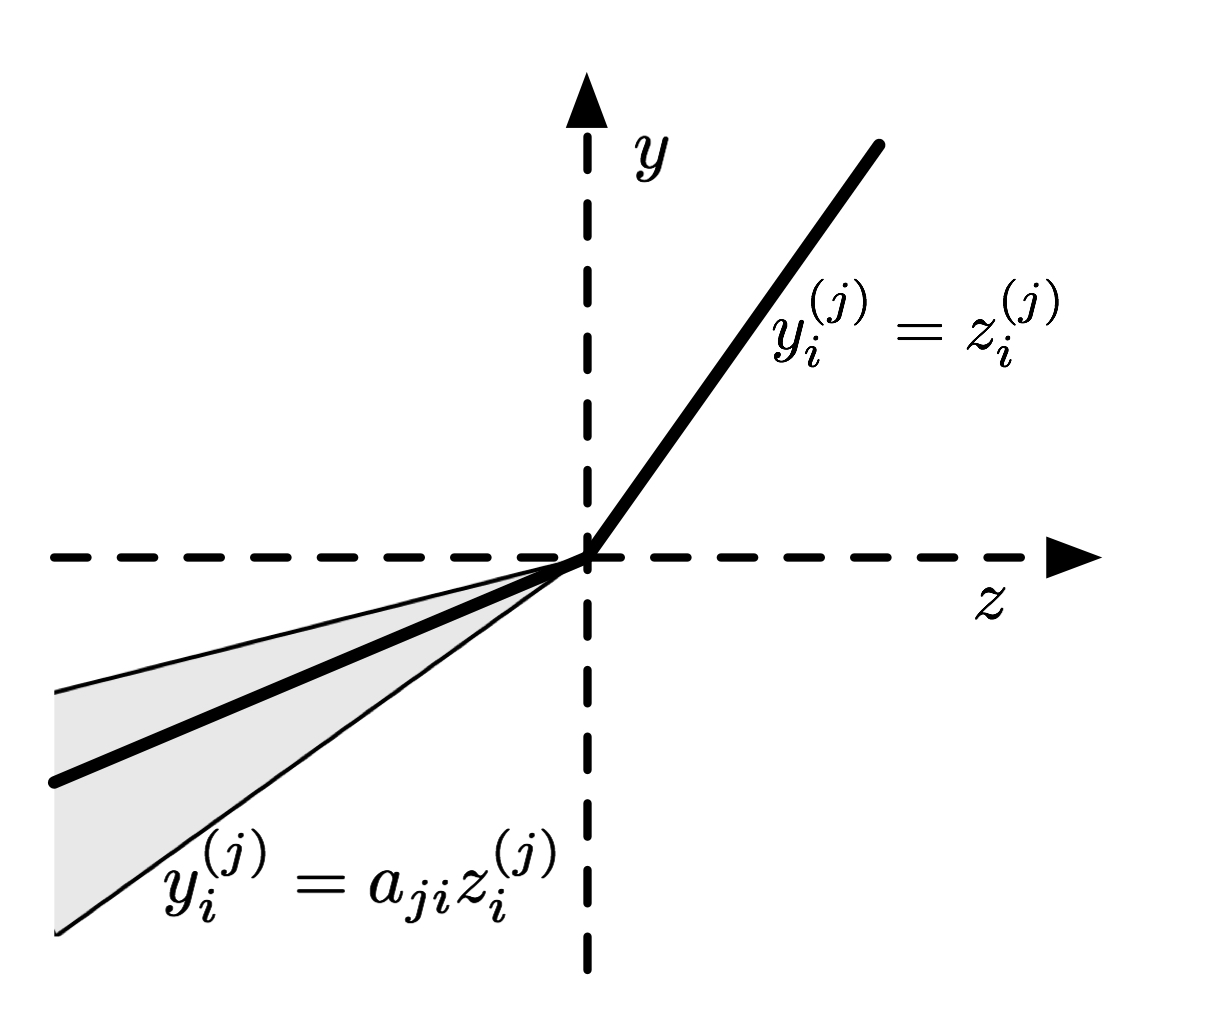
\includegraphics[height=30mm,width=\textwidth]{ch02_06_03.jpg}
			\caption{RReLU}
			\label{fig:RReLU}	
		\end{subfigure}&
		\begin{subfigure}[c]{0.25\textwidth}
			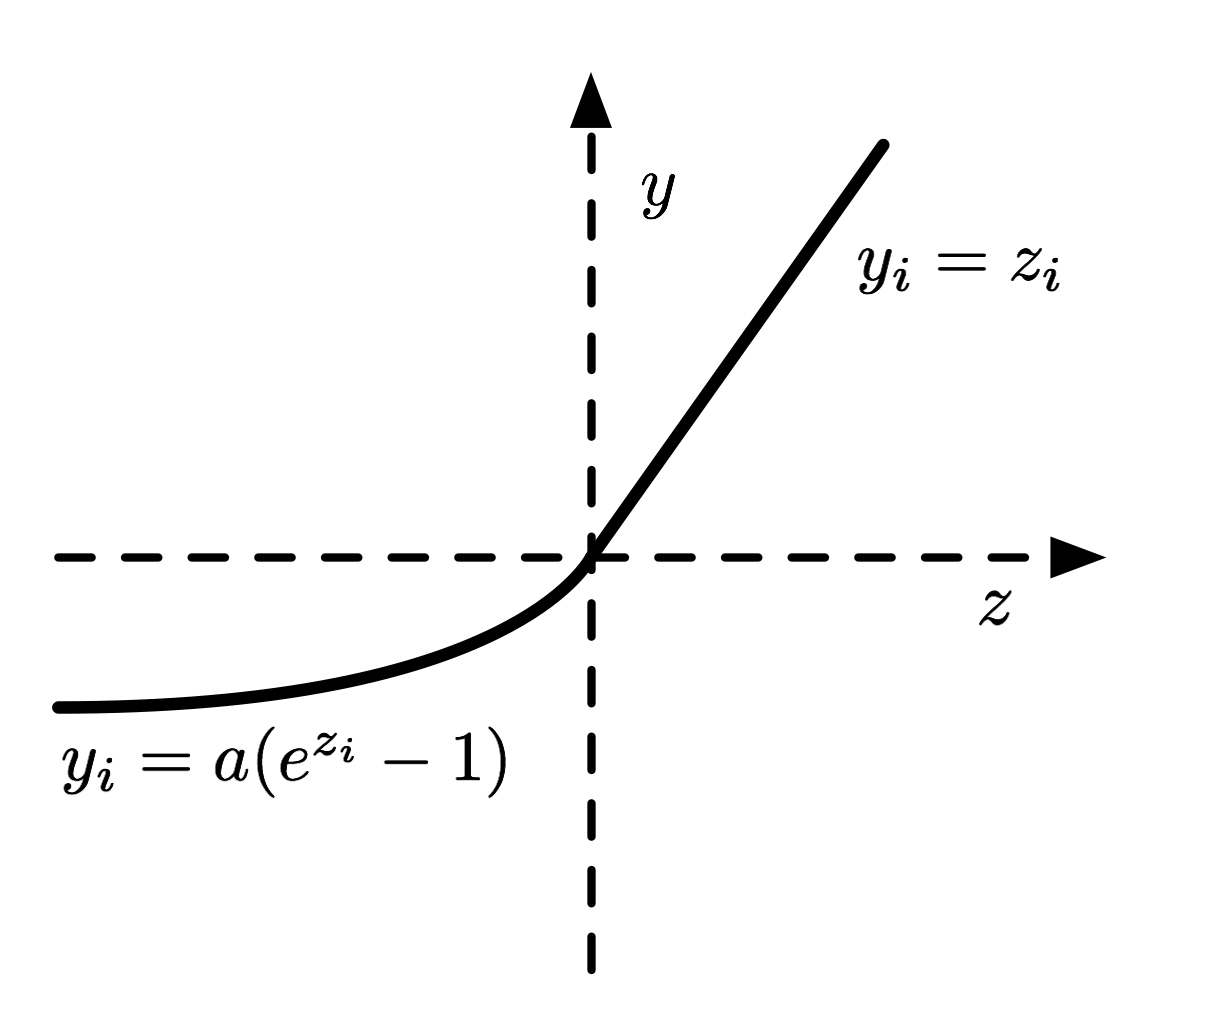
\includegraphics[height=30mm,width=\textwidth]{ch02_06_04.jpg}
			\caption{ELU}
			\label{fig:ELU}	
		\end{subfigure}				
	\end{tabular}    
	\caption[各种激活函数比较图]{ReLU,LReLU,PReLU,RRELU和ELU之间的比较,参数$\lambda $对于Leaky ReLU,是凭经验预定义的。对于PReLU是从训练数据中学习的。对于RReLU是一个随机变量,它是从训练中给定的均匀分布中抽取的,并在测试中保持固定。对于ELU是凭经验预定义的。}
	\label{fig:RRELU}
\end{figure}

\subsubsection{Maxout}
Maxout\cite{Goodfellow2014Generative}是一种替代性的非线性函数,能够近似任意连续函数,可以在每个空间位置获得跨多个通道的最大响应,函数定义如下:
$ a_{i,j,k}=\max_{k \in[1,K]}z_{i,j,k}$,其中$ z_{i,j,k} $是第$ i $通道的特征映射。由于ReLU实际上是maxout的一个特例,Maxout享有ReLU的所有好处,但参数会相应加倍。
\subsection{损失函数}
深度神经网络设计中的一个重要方面是损失函数的选择,损失函数是模型对数据拟合程度的反映,为特定任务选择合适的损失函数非常重要。我们在本小节中介绍三个有代表性的部分:softmax损失,铰链损失和对比损失。

\subsubsection{Softmax 损失}
Softmax损失结合softmax函数和交叉熵损失,是多项式逻辑损失和softmax的组合。给定训练$\{(x^{(i)}, y^{(i)}); i\in {1,\dots,N}, y^{(i)}\in {0,\dots,K-1}\}$,其中$ x ^ {(i)} $是$ i $ 输入图像区域,$ y^{(i)} $是它的类标签。第$ i $ 输入的第$ j $类的预测$ a_j ^ {(i)} $用以下softmax函数进行变换:
\begin{equation}
\label{eq:softmax}
p_j^{i} =e^{a_j^{(i)}}/{\sum_{l=0}^{K-1}e^{a_l^{(i)}}}
\end{equation}
Softmax将预测变成非负值,并将它们归一化以获得类别概率分布。这种概率预测用于计算多元逻辑损失,如下所示:

\begin{equation}
\label{eq:softmaxloss}
\begin{aligned}
\mathcal{L}_{softmax} =-\frac{1}{N}[\sum_{i=1}^{N}\sum_{j=0}^{K-1}1\{y^{(i)}=j\}\mathrm{log} p_j^{i}]
\end{aligned}
\end{equation}

\subsubsection{铰链损失}
铰链(Hinge)损失通常用于训练最大间隔的分类器,如支持向量机(Support Vector Machine,SVM)。多类SVM的铰链损失函数由公式(\ref{eq:L1_SVM_ml})定义,其中$ x_n $ 是给定的特征向量,而$ \ell_n \in [0,1,2,...,K-1] $指示$ K $类中的正确类标签。

\begin{equation} \label{eq:L1_SVM_ml}
\begin{aligned}
& \mathcal{L}_{Hinge} =\frac{1}{N}\sum_{n=1}^{N}\sum_{k=0}^{K-1}[\mathrm{max}(0,1-\delta(\ell_n,k)w^T x_n)]^p  \\
& \delta(\ell_n,k)=
\begin{cases}
1, & \text{if $\ell_n = k$} \\
-1, & \text{if $\ell_n \ne k$}
\end{cases}
\end{aligned}
\end{equation}

注意如果$ p = 1 $,公式(\ref{eq:L1_SVM_ml})是$ L_1 $损失,而如果$ p = 2 $,则是平方铰链损失$ L_2$。

\subsubsection{对比损失}
对比(Contrastive)损失\cite{Shaham2017Learning}常用于训练孪生多通路网络,属于弱监督方法,用于从标记为匹配或不匹配的数据实例对中学习相似性度量。 给定第$i$对数据$(x_{\alpha} ^{(i)},x_{\beta} ^{(i)})$,令$(z_{\alpha} ^{(i,l)},z_{\beta} ^{(i,l)})$表示其对应的第$l$个($l \in [1,\dots,L]$)层的输出对。图像对通过两个相同的CNN分别传递,并将最终图层的特征向量送入到损失函数,对比损失$ \mathcal {L} _l $被定义为:

\begin{equation}
\begin{aligned}
\label{ContrastiveLoss}
 \mathcal{L}_{contrastive}= \frac{1}{2N}\sum_{n=1}^{N}\sum_{l=1}^{L}(y)d^{(i,L)} + (1-y)\max(\mathrm{m}-d^{(i,L)}, 0) 
\end{aligned}
\end{equation}
其中$d^{(i,L)} = ||z_{\alpha}^{(i,l)} - z_{\beta}^{(i,l)}||_2^2$,是$ z ^{(i,l)}_\alpha $和$ z^{(i,l)}_\beta $之间的相似度,$ m $是影响非匹配对的边界参数。如果$(x_{\alpha} ^{(i)},x_{\beta} ^{(i)})$是匹配的对,那么$ y = 1 $。否则,$ y = 0 $。这种损失函数也被称为单边界参数损失函数。Lin等\cite{Zhu2016b}利用这种单边界损失函数在所有对上对网络进行训练时,会导致检索结果急剧下降。同时,仅在非匹配对上进行内部调整时,性能得到更好的保留。 这表明处理丢失函数中的匹配对是造成丢失的原因。 虽然非匹配对的召回率是稳定的,但处理匹配对是召回率下降的主要原因。 为了解决这个问题提出了一个双边界损失函数,它为匹配对添加了另一个边界参数。定义为:

\begin{equation}
\label{DMContrastiveLoss}
\mathcal{L}_{doublecontrastive}= \frac{1}{2N}\sum_{n=1}^{N}\sum_{l=1}^{L}(y)\max(d^{(i,L)}-\mathrm{m}_1,0) + (1-y)\max(\mathrm{m}_2-d^{(i,L)}, 0)
\end{equation}
\subsection{优化方法}
在本小节中,我们将讨论优化CNN训练的一些关键技术。

\subsubsection{权重初始化}
通常深度CNN模型具有大量的参数并且损失函数是非凸的,导致难以训练。为了实现训练中的快速收敛,正确的初始化是最重要的先决条件之一。偏置参数可以初始化为零,而权重参数的设置需打破同一层隐藏单元之间的对称性。例如,如果我们简单地将所有权重初始化为相同的值,例如0或1,那么同一层的每个隐藏单元将得到完全相同的信号。
有些启发式方法可用于选择权重的初始大小,最常用的初始化方法是根据高斯或均匀分布随机设置权重。Glorot和Bengio\cite{Glorot2010}提出初始化$m$个输入$n$个输出可根据零均值和特定方差的分布设置权重:$ Var(W_{i,j})~ \sqrt{6} / \sqrt{m + n} $,也被称为“Xavier”。但是初始化时强加的性质可能在学习开始进行后不能保持;可能成功提高了优化速度,但意外地增大了泛化误差,这些初始化方法往往不会带来最佳效果。在实践中,我们通常需要将权重范围视为超参数进行调参估计。

\subsubsection{随机梯度下降}\label{SGD_optimization}
一般使用批梯度下降(stochastic gradient descent,SGD)来更新模型参数,采用反向传播算法计算损失函数的梯度。梯度下降算法将目标$ J(\theta)$的参数$ \theta $更新为$ \theta_{t + 1} = \theta_t - \alpha \nabla_\theta E [J(\theta_t)] $,其中$ E [J(\theta_t)] $是整个训练集上$ J(\theta)$的期望值,$ \alpha $是学习率。随机梯度下降根据单个随机选取的示例$(x ^ {(t)},y ^ {(t)})$进行梯度更新:
\begin{equation}
\label{eq:SGD}
\theta_{t+1} = \theta_t - \mu_t \nabla_\theta J(\theta_t; x^{(t)},y^{(t)})
\end{equation}

实际上,SGD中的每个参数更新都是针对小批量数据(mini-batch)而不是单个示例,这可以帮助减少参数更新中的变化并且可以导致更稳定的收敛性。收敛速度由学习率$ \mu_t $控制。在面对小而连续的梯度但是含有很多噪声的时候,带动量(Momentum)SGD算法可以很好的加速学习为了加速训练使当前更新梯度取决于历史梯度在相关方向上累积速度向量信息,经典的带动量SGD更新由下式给出:
\begin{equation}    \label{eq:mSGD}
\begin{aligned}
   & v_{t+1} = \theta_t - \mu_t \nabla_\theta J(\theta_t; x^{(t)},y^{(t)})\\
   & \theta_{t+1} = \theta_t +v_{t+1} 
\end{aligned}
\end{equation}
其中$v_{t+1}$是当前速度矢量,是通常设置动量衰减参数$\mu$为0.9。 在梯度下降优化中使用动量的另一种方式Nesterov\cite{Krizhevsky2012}:
\begin{equation}
    \label{eq:nSGD}
    v_{t+1} = \gamma v_t - \mu_t \nabla_\theta J(\theta_t; x^{(t)},y^{(t)})
\end{equation}
\ref{eq:nSGD}首先计算当前梯度,然后沿更新的累积梯度方向移动,与经典动量\ref{eq:mSGD}相比,Nesterov首先沿先前累积梯度的方向移动vt,计算梯度,然后进行梯度更新。这种预期的更新可以防止优化移动太快,并获得更好的性能。一种常用的方法是使用小的恒定学习速率,在初始阶段给出稳定的收敛,然后随着收敛速度的减慢而降低学习速率。除了这种人工手动设置学习率的方法之外,还有很多自适应学习率的方法,如Adam\cite{Kingma2014Adam}利用梯度的一阶矩估计和二阶矩估计动态调整每个参数的学习率。此外,并行化的SGD方法能够提高SGD以适合并行的大规模机器学习。

\subsubsection{批量归一化}
批量归一化(Batch Normalization)\cite{Ioffe2014Batch}的提出旨在加速深度神经网络的整个训练过程。他们认为内部协变量偏移,即深度网络内部节点分布的变化将会减慢网络训练的速度。为此提出了一种称为批量归一化的有效方法来部分缓解这种现象。它通过归一化数据使其服从标准高斯分布来修复了各层输入的方式和差异。批量归一化可以理解为在网络的每一层之前都做预处理,只是这种操作以另一种方式与网络集成在了一起。除了加速训练外,批量归一化还使我们能够使用更高的学习速率而不存在发散风险,并且可以通过防止网络陷入饱和模式来使用饱和非线性。
\subsection{正则化方法}
过拟合在深层CNN中是一个不容忽视的问题,可以通过正则化来有效降低过度拟合问题。在下面的小节中,我们介绍一些有效的正则化技术。
\subsubsection{$p$范数正则化}
正则化通过增加惩罚模型复杂性的额外项来修改目标函数,若损失函数为$L(\theta; x; y)$,则正则化损失将为:
\begin{equation}
E(\theta ; x; y)= L(\theta ; x; y)+\lambda R(\theta ) 
\end{equation}
其中$R(\theta)$是正则化项,并且$\lambda$是正则化项参数。
$p$-范数正则化函数通常用作$R(\theta)=\sum_j||\theta_j||_p^p$,当$p=1$,$p$-范数是凸的,这使得目标函数更容易优化,并使这个函数具有稀疏性,使得参数变小倾向接近零。对于$p = 2$,“2-范数正则化”通常称为“权重衰减”,使得参数更平均; 当$p<1$时,$p$-范数正则化更多地利用了权重的稀疏效应,但却导致了非凸函数。
\subsubsection{随机失活}
\label{Section Dropout}
随机失活(Dropout)\cite{Srivastava2014a} 提供了一大类模型的正则化方法,其可以被认为是集成大量深层神经网络的实用Bagging方法,能够训练和评估指数级数量的神经网络,计算方便但功能强大。在训练的时候,随机失活的实现方法是让神经元以超参数$p$的概率被激活或者被设置为0。在训练过程中,随机失活可以被认为是对完整的神经网络抽样出一些子集,每次基于输入数据只更新子网络的参数(然而,数量巨大的子网络们并不是相互独立的,因为它们都共享参数)。在测试过程中不使用随机失活,可以理解为是对数量巨大的子网络们做了模型集成,以此来计算出一个平均的预测。

研究指出在使用费舍尔信息矩阵(fisher information matrix)的对角逆矩阵的期望对特征进行数值范围调整后,再进行L2正则化这一操作,与随机失活正则化是一阶等价的。而DropConnect\cite{Wan2013Regularization}将Dropout的思想更进一步改进,DropConnect不是将神经元的输出设置为零,而是以概率$ p $选择完全连接层的权重$ W $设置为零。\figurename {\ref{fig:CNN_DropConnect}}说明了无Dropout,Dropout和DropConnect网络之间的差异。

\begin{figure}
	\centering
	\begin{tabular}[c]{ccc}
		\begin{subfigure}[c]{0.27\textwidth}
			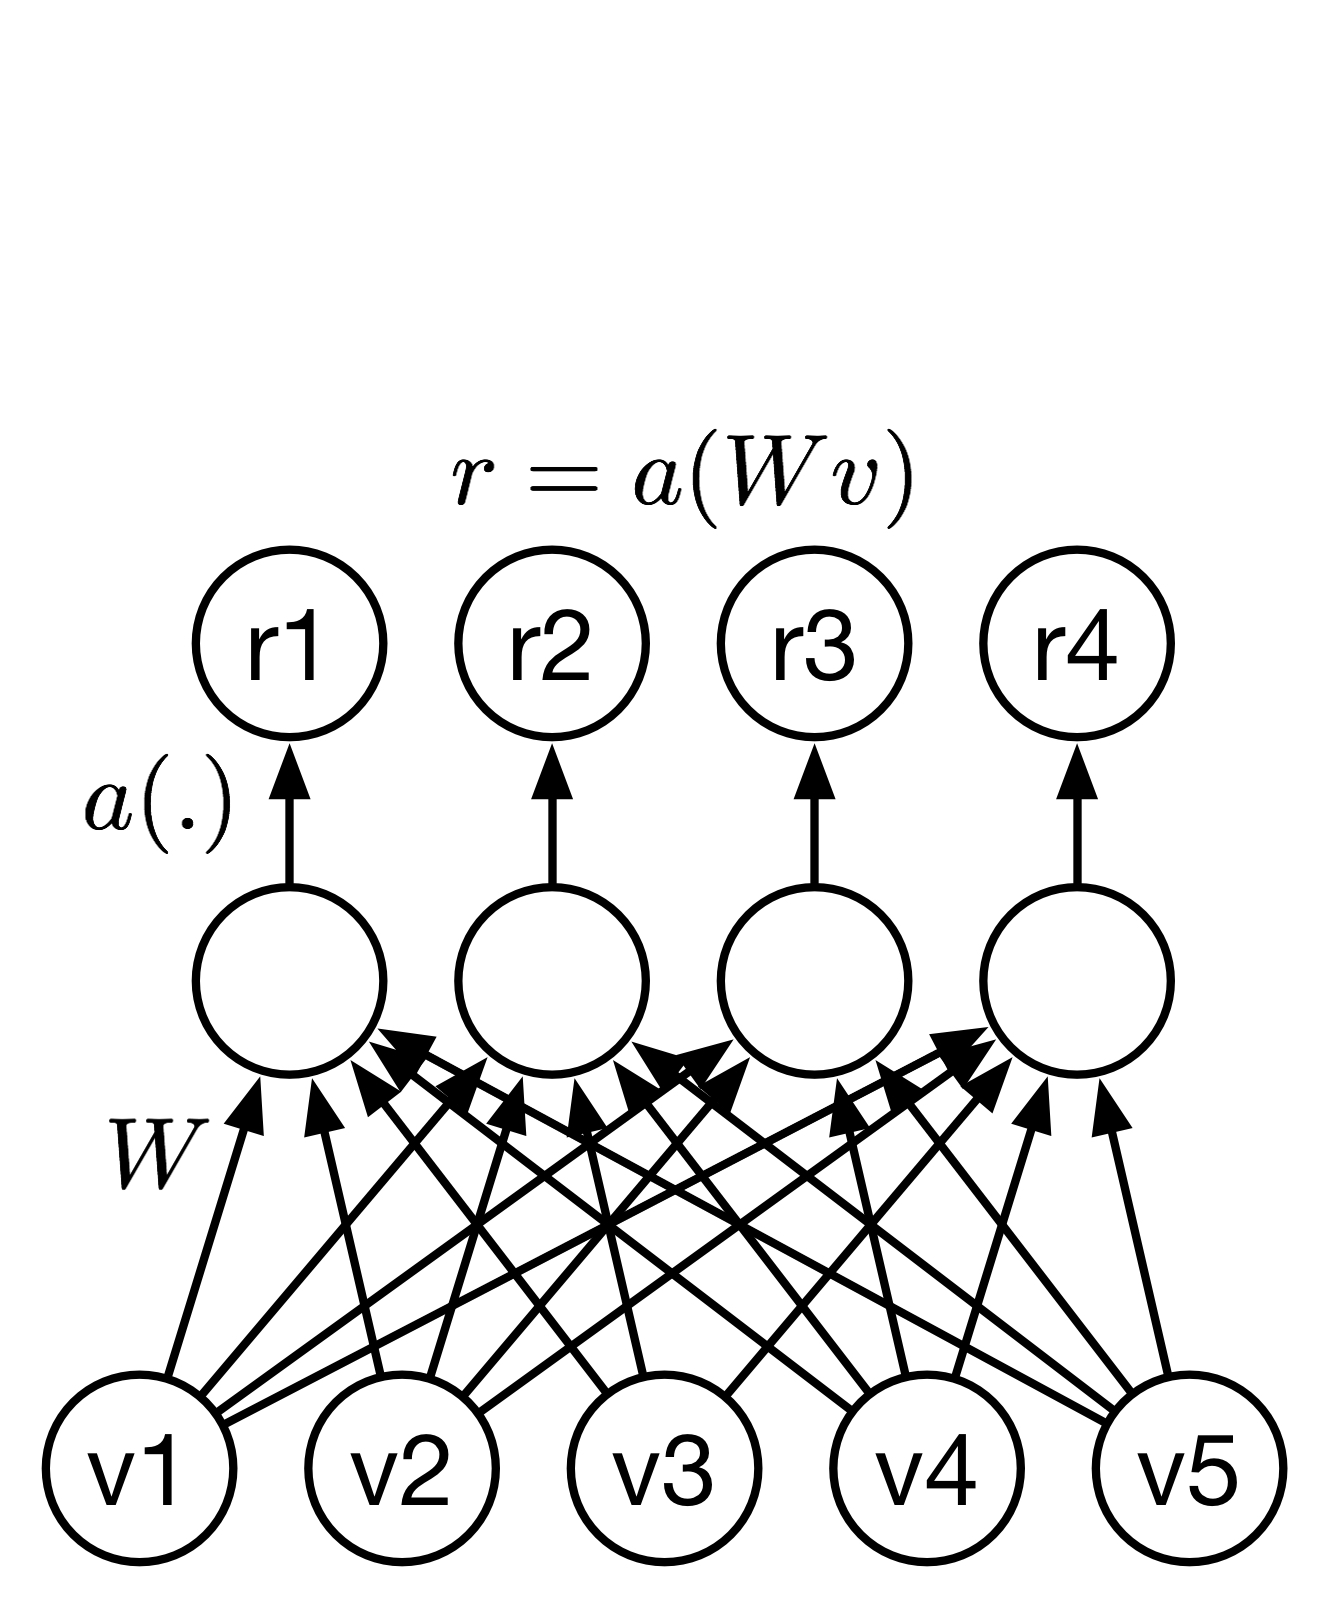
\includegraphics[width=\textwidth]{ch02_07_01.jpg}
			\caption{No-Drop}
			\label{fig:nodrop}
		\end{subfigure}&
		\begin{subfigure}[c]{0.27\textwidth}
			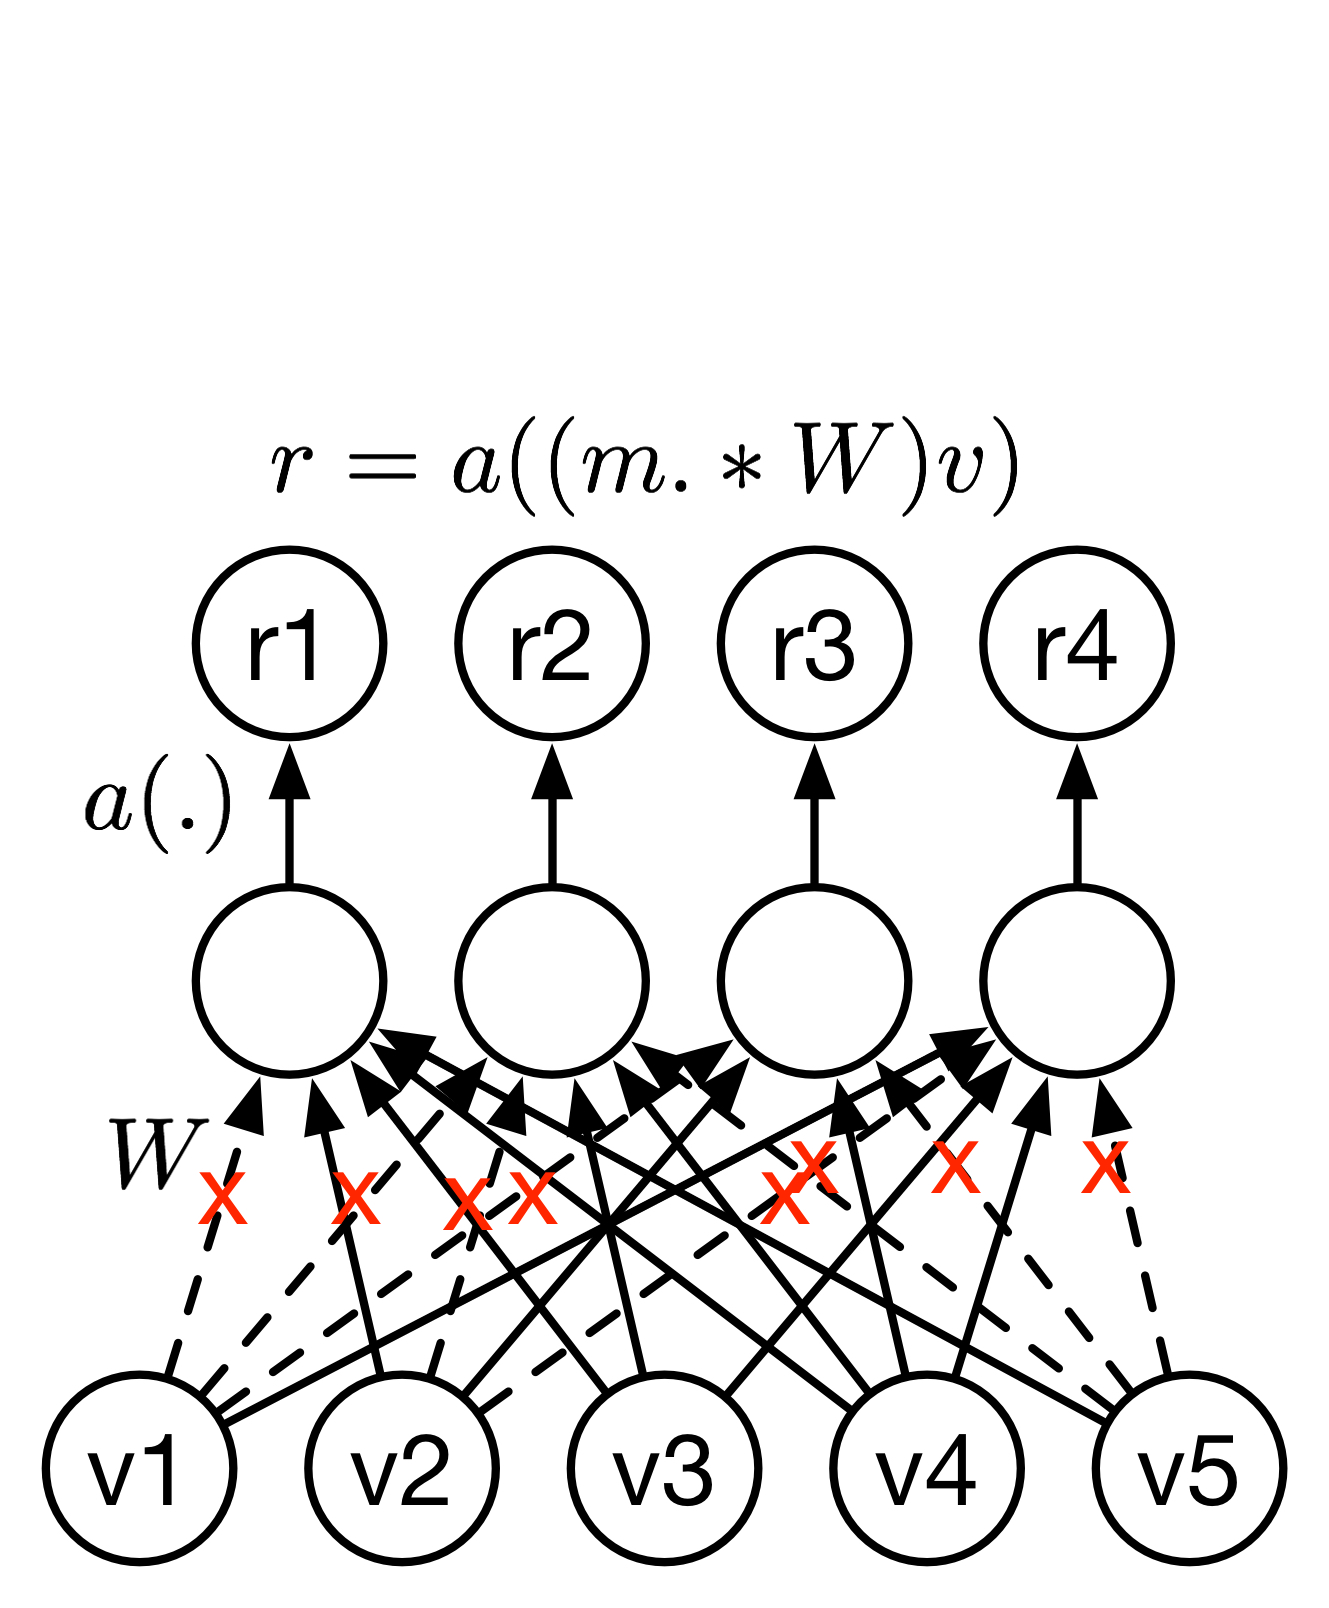
\includegraphics[width=\textwidth]{ch02_07_02.jpg}
			\caption{DropOut}
			\label{fig:dropout}
		\end{subfigure}&
		\begin{subfigure}[c]{0.27\textwidth}
			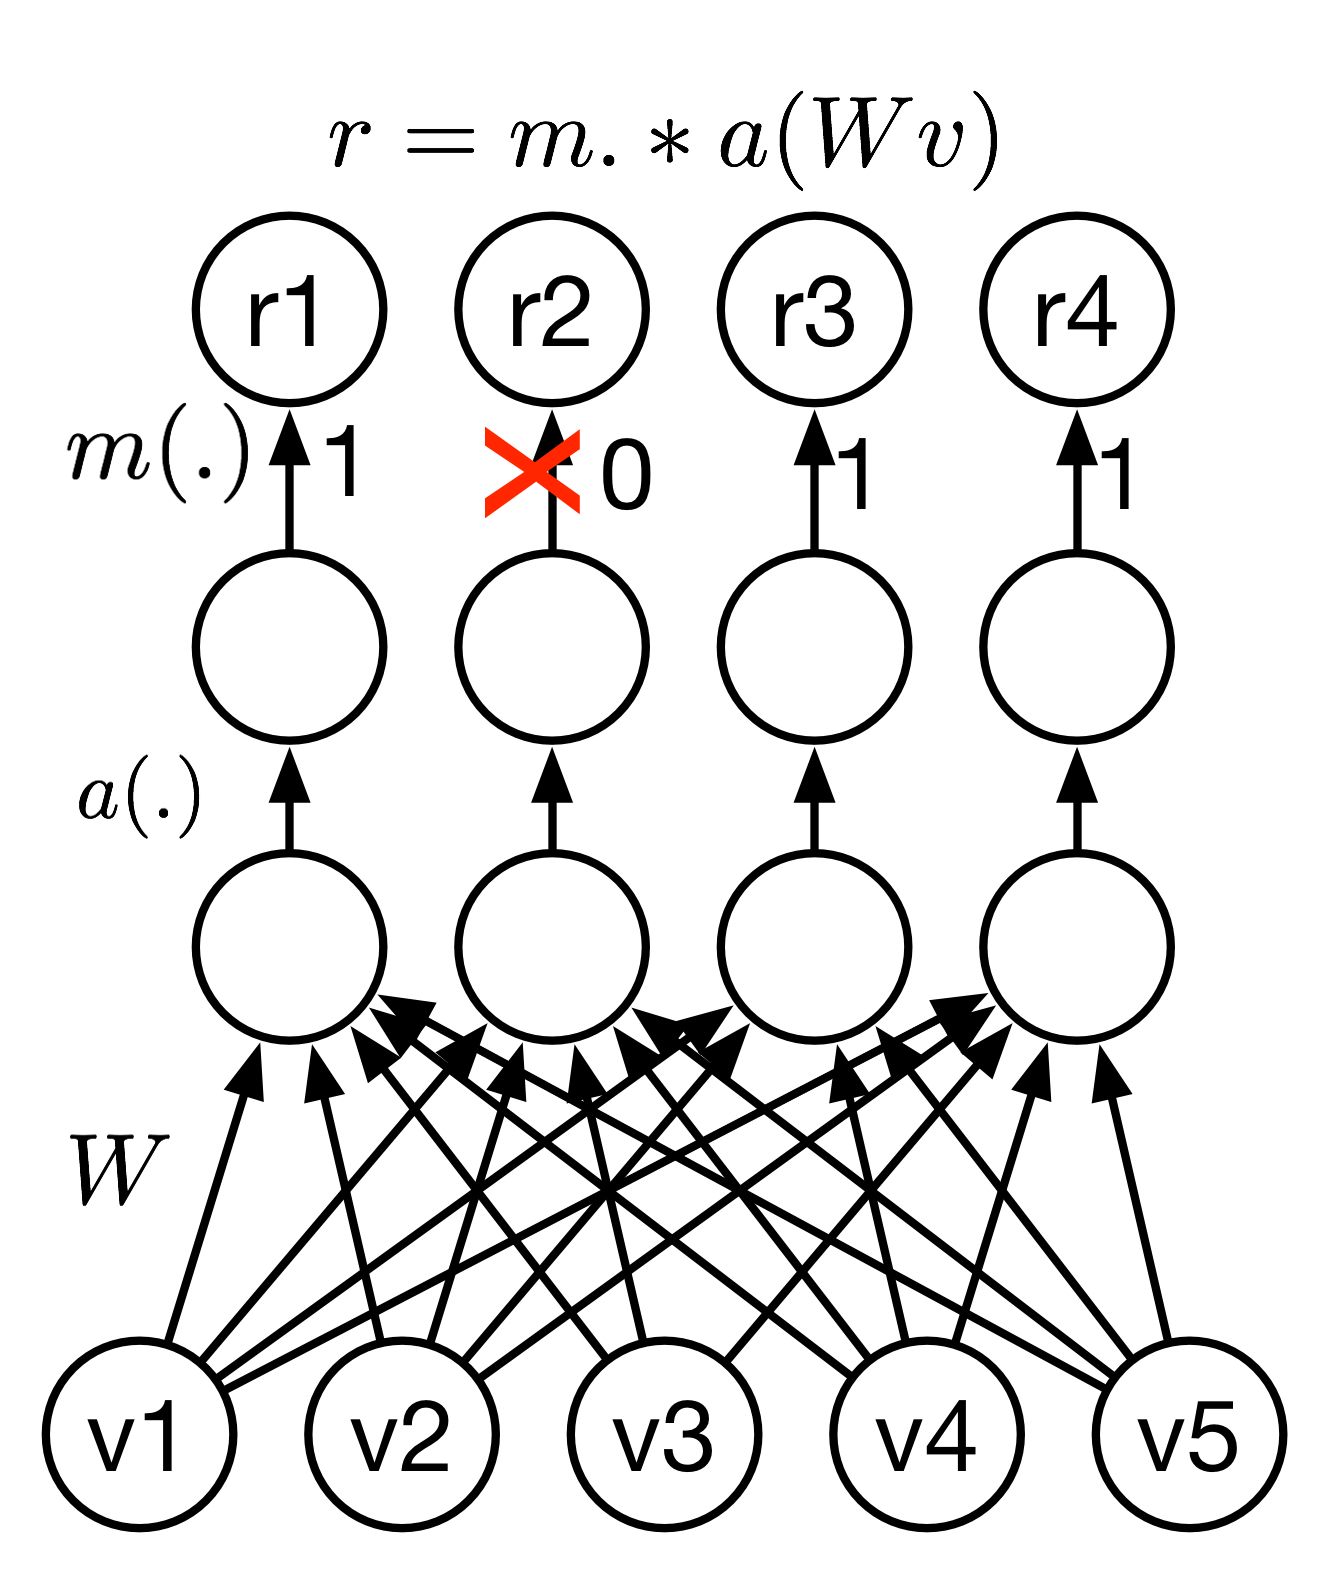
\includegraphics[width=\textwidth]{ch02_07_03.jpg}
			\caption{DropConnect}
			\label{fig:dropconnect}	
		\end{subfigure}			
	\end{tabular}    
	\caption{无Dropout网络,DropOut网络和DropConnect网络的图示。}
	\label{fig:CNN_DropConnect}
\end{figure}

\section{小结与讨论}

本章首先对学习算法和神经网络基本方法进行了梳理,包括卷积神经网络和深度卷积神经网络模型进行了分析,进一步对无监督深度学习进行了概述。同时对深度学习应用于医学图像中涉及的分类、检测和分割应用算法从原理上进行了分析。最后对深度学习中相关核心技术了描述,涉及激活函数、损失函数、优化方法和正则化。 
\chapter{特征表示的高层语义应用}
\label{chap:classification}

\section{超声心动图切面的自动识别方法}
在心脏病常规临床检查中,二维实时超声心动图常用于评测心脏的结构和功能。临床超声检查通常主要包括三个步骤:探头扫描不同位置,选取标准切面和对标准切面的测量和诊断\citep{Chen2015}。其中,医师总结出来能更好辅助分析心脏功能结 构的特定位置和角度的超声心动图称为标准切面,其正确快 速选取不仅对临床诊断具有至关重要的意义,也为病例研究 提供比较依据。标准切面的自动识别是超声心动图智能分析和测量的基础。与自然图像相比,医学超声成像质量差,存在斑点噪声和伪影;并且各标准切面类内、类间差异大,使得标准切面的识别成为一个非常具有挑战性的问题。

目前的研究主要集中在利用机器学习和图像处理等方法,进行超声心动图的自动识别、检索及切面内组织结构的定位和分割等。针对超声心动图的自动识别,2004年Shahram 等\citep{Ebadollahi2004}首次提出采用马尔科夫随机场,设计通用腔室模板检测 心脏腔室来辅助三类标准切面识别,但需额外信号来指定处 于舒张末期(End–Diastolic,ED)的切面。同样利用处于ED的标准切面,Kevin等\citep{KevinZhou2006}基于多类别提升算法框架,提取哈尔矩形特征训练弱分类器,同样需要检测心脏腔室的空间位置,辅助四类标准切面识别。基于降低特征维度的两层级联方法,把标准切面分类成心尖和胸骨旁两大类,然后进一步区分四类标准切面视频\citep{Otey2006,Roy2006b}。在文献\citepns{Ebadollahi2004}工作基础上整合局部和全局模板特征,利用多类逻辑提升分类算法,并指出能扩展到任意标准切面\citep{Park2007a}。在对心脏的循环跳动的时空信息进行统计分析的基础上,利用主动外观模型对形状和纹理进行建模,统计追踪一个心动周期并投影到运动空间进行分类\citep{Beymer2008},该方法处理的视频序列。把标准切面视为不同场景,提取低层全局特征来表征不同切面,利用改进核支持向量机进行分类\citep{Wu2014c}。这些方法可以归纳为两个阶段:首先根据先验人为设计特征来表征图像;然后利用机器学习中不同分类方法对特征向量进行建模分析得到分类器。然而受限于‘语义鸿沟’问题,根据特定先验人为设计特征,如大多数方法都针对心动周期的某个特定时刻的切面(如ED),会导致模型泛化性能差。

近来,深度卷积神经网络(Convolutional Neural Network,CNN)在大规模自然图像数据集(如ImageNet\citep{Deng2009ImageNet})上,识别性能远超传统方法\citep{Krizhevsky2012}。主要得益于深度学习利用大量标注数据从图像原始像素出发,逐层分级学习中高层的抽象语义特征\citep{Sharif2014}。
当前实践中由于深度学习需要大量的标注数据,所以仅在少数医学任务中取得有限的成功应用,且对深度模型的鲁棒性和有效性也缺乏详尽分析。Chen等\citep{Chen2015}利用CNN结合领域知识,在胎儿超声心动图标准切面的自动识别问题中取得良好的识别效果,但胎儿跟成人超声心动图差异大,具有很大特殊性。Bar等\citep{Bar2015Chest}利用自然图像训练的模型对胸腔X-射线图像进行特征提取并结合全局特征\citep{Oliva2001}得到最优检测结果,并没有对特定医学数据进行迁移训练,仅是作为特征提取器。Margeta等\citep{Margeta2015}针对心脏核磁共振图像利用微调迁移从自然图像学习的模型,但没对模型有效性进行分析。

目前深度CNN模型的理论分析工作还不是很完善,能自动学习语义特征的工作机理还是个“黑箱”。对于不同的模型的比较除了准确率之外并没有很好的评价方法,优异的泛化能力从何而来仍是个开放问题。一些工作\citep{simonyan14deep,Mahendran2015,Zeiler2014,Zhou2015}通过可视化各层激活值和卷积核来更好理解深度CNN。对在给定数据集上训练得到的深度CNN网络模型,Simonyan等\citep{simonyan14deep}用反卷积来可视化每个神经元的最大激活值。Mahendran等\citep{Mahendran2015}通过对学习到的每层的特征编码进行反编码,建立每层特征编码和原图像的映射关系。Zeiler等\citep{Zeiler2014}试图通过梯度上升方法迭代寻找图像使得最大化激活某个或某些特定的神经元。神经元对图像每个像素的梯度描述了当前像素的怎样改变能影响分类结果。前三个方法均是对已训练的模型进行分析,而类激活映射图(Class Activation Maps,CAM)方法\citep{Zhou2015}用全局平均池化层代替全连接层改进训练过程,分类性能虽略有降低,但能指示出特定类别的显著性判别区域,能很好的解释模型的有效性。

本文提出一种基于深度CNN自动识别超声心动图标准切面的方法(Deep Echocardiogram,Deep-Echo):
1)引入空间金字塔平均池化层代替全连接层,一方面大大减少模型参数,降低过拟合风险;另一方面网络结构变为全卷积网络,使得不用限制输入图像尺寸大小,这对医学超声图像更为重要。2)为验证该算法的鲁棒性和有效性,针对数据集进行详尽实验,研究分析了深度学习方法的高识别率和优异泛化能力的原因。
 
\section{Deep-Echo模型}

将分别从如何构建全卷积网络、全局空间金字塔平均池化层、将类别显著性图纳入可视化过程、如何扩增数据等方面介绍提出的Deep-Echo模型。
\subsection{全卷积的网络}

与GoogLeNet模型\citep{Szegedy2015}、ResNet模型\citep{he15}类似,使用多层卷积层(每层包括ReLU层、BN层和Pooling层),用全局平均池化操作替代全连接层。Deep-Echo模型结构中对最后卷积层输出的特征图,用金字塔平均池化层\citep{He2015spp}代替最大化池化层和全连接层。最后一层输出单元数目为类别的数目,由于实验采用的标准切面有七个类别,因此最后一层输出7,依次对应相应的类别,采用交叉熵损失函数加L2正则化。卷积核数目从64开始,每经过一次最大池化层,卷积核数目翻倍,直到512为止。学习率初始化为0.01。具体实验步骤和参数设置见后文实验部分。整个网络结构如图\ref{fig:ch03_02}所示。

\begin{figure}[!htbp]
\centering
%trim option's parameter order: left bottom right top
%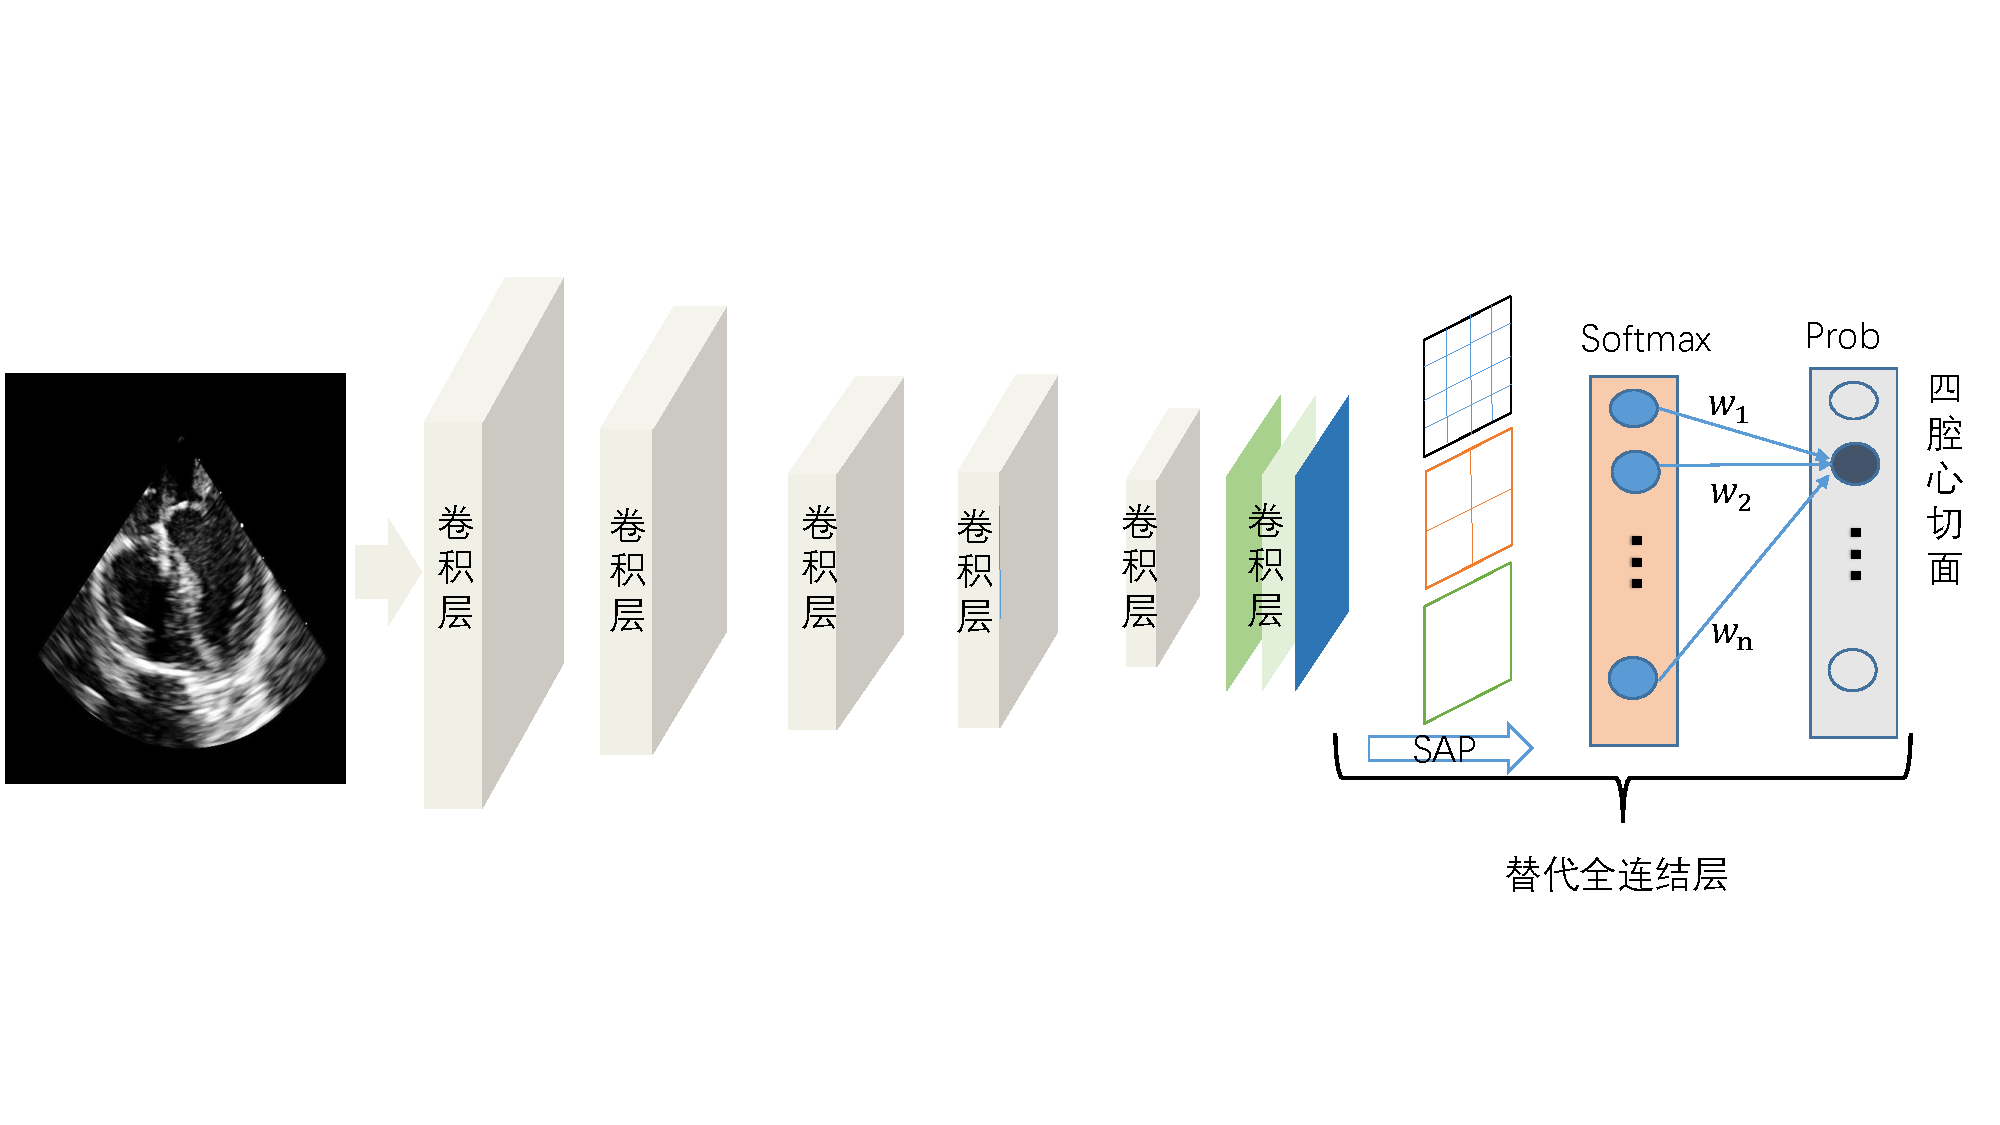
\includegraphics[trim = 30mm 0mm 30mm 0mm, clip, width=0.45\textwidth]{ch03_02}
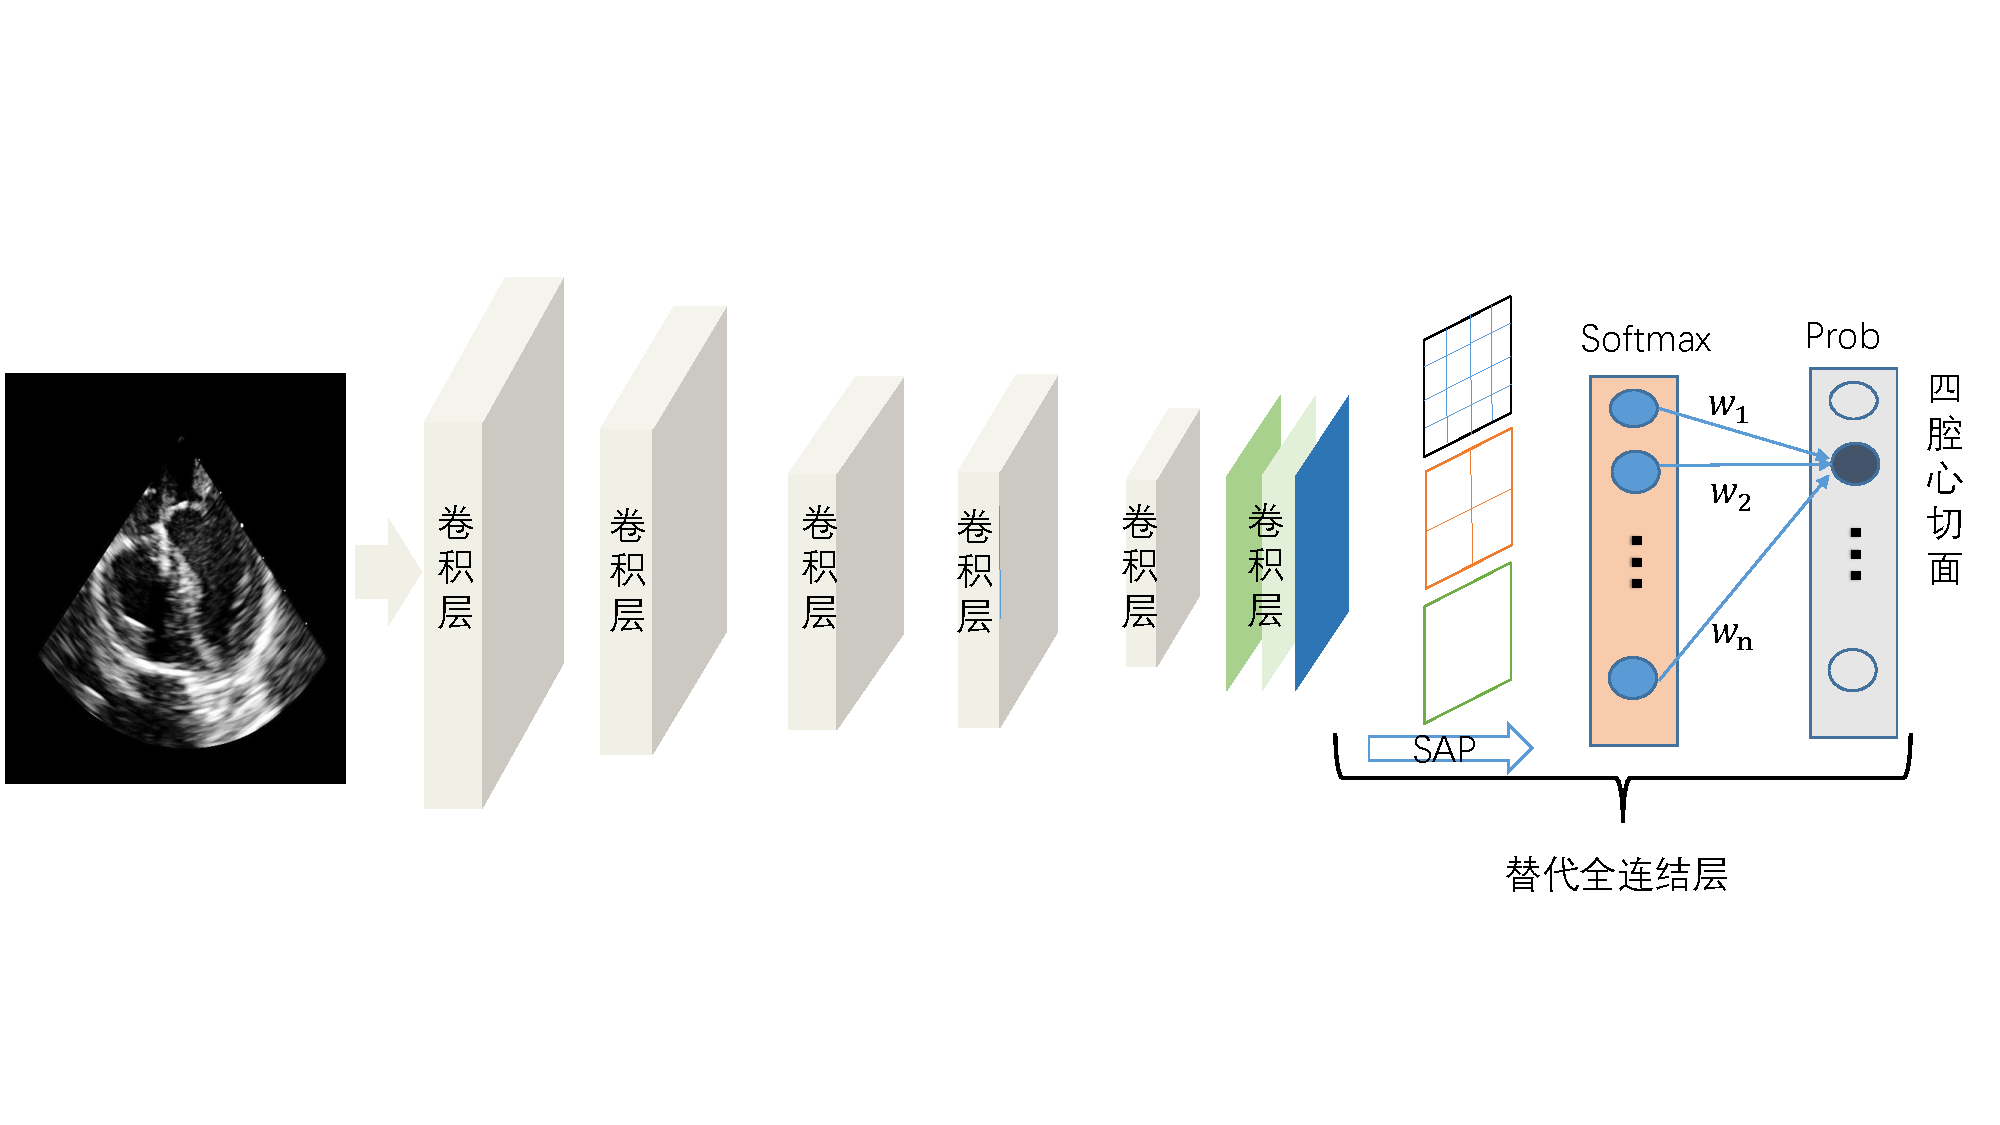
\includegraphics[width=0.9\textwidth]{ch03_01}
\caption{Deep-Echo模型结构示意图}
\label{fig:ch03_01}
\end{figure}

\subsection{空间金字塔均值池化层}

针对深度CNN模型中全连接层的两个缺点:全连接层丢失了空间信息,限制了 CNN 只能接受固定尺度的输入,一般只能通过图像尺度归一化的方法来处理不同尺度的输入图像,且使得模型可视化变得不可解释;全连接层参数拥有大约90\%的模型参数,如AlexNet模型\citep{Krizhevsky2012}和VGG16模型\citep{Chatfield2014}中全连接层参数占全部参数分别为38M/61M和103M/138M,从而导致模型更容易过拟合\citep{Szegedy2015}。
为解决这两个问题,He等提出空间金字塔池化 (Spatial Pyramid Pooling,SPP)方法\citep{He2015spp}。SPP通过使用多个不同大小的池化操作保证固定的特征向量输出,从而允许 CNN 接受任何尺度的输入,增加了模型的尺度不变性,抑制过拟合。与传统的全连接层不同,对每个特征图一整张图片进行多尺度的空间金字塔均值池化,这样每张特征图都可以得到多个尺度的输出。本文方法跟空间金字塔池化网络类似都是三个尺度的空间金字塔池化(1×1,2×2,4×4),其差异在于后不再接多个全连接层,同时用平均池化代替最大化池化,目的在于方便可视化模型的空间位置信息。
\section{微调迁移学习}

利用深度学习进行超声心动图的标准切面识别,仍存在针对小数据量直接训练是否会出现过拟合问题;能否跨领域进行迁移学习,即在自然图像数据集上训练得到的模型能否微调应用到跨领域的超声心动图上。文献\citepns{Zhou2015}中指出,用全局平均池化代替全连接层直接随机初始化,从头开始训练模型收敛困难且分类性能下降,故对现有模型进行改造,即针对在自然图像集上预先训练得到的模型如,Alexnet模型等,变换最后的输出层为所述金字塔平均池化结构,调小学习率后在超声心动图标准切面数据上进行微调迁移学习。

训练时,由于超声心动图的特殊性,人工标注费时费力,对数据集进行扩增能降低人工标注的需求。但扩增数据需注意不能打乱标准切面图像内在的局部结构,因此对切面数据只进行水平镜像翻转和旋转。通过引入BN归一化层能减轻对Dropout的依赖,提高泛化能力,并且本文直接去掉全连接层,故并未采用Dropout技术。
迁移学习时,由于深度模型中低层的卷积核是跟人类视觉的初级细胞很类似,因此是可以直接迁移复用,高层要针对目标学习判别性信息需进行重新学习\citep{Zhou2015}。针对超声心动图的实验支持这样的结论,不同模型的分类准确率都很高,具体实验见后文实验部分。但对于计算机医学辅助诊断而言,模型怎样决策判断比分类准确率更重要。即需解释模型为什么有效和优异的泛化能力从何而来。
\section{类别显著激活映射图}

前文所提模型能高效提取超声心动图标准切面的特征,对超声心动图的单扇形和双扇形标准切面都能很好的识别,甚至对互联网上随意选取的标准切面也能识别。但对模型的有效性和解释性缺乏有力分析,使得对模型决策判断的可信性产生怀疑。
针对超声心动图,采用\citepns{Zhou2015}提出可视化分析的方法,将其和空间金字塔平均池化结合。对给定图像,$f_{j}(x,y)$ 表示卷积层(x,y)位置上第j个神经元的激活值,对第j神经元的平均池化操作结果对给定类别k的得分函数S:
\begin{equation} \label{eq:s}
     S_{k}=\sum_{j}w_{j}^{k}\sum_{x,y}f_{j}(x,y)
\end{equation}	    
其中 $w_{j}^{k}$ 是第j 个神经元和第k 类的连接权重,后接多类多元逻辑损失层,然后由公式\ref{eq:m}可得定义类别激活映射图:	
  	      \begin{equation} \label{eq:m}
     M_{k}=\sum_{j}w_{j}^{k}f_{j}(x,y)
\end{equation}
其中,$M_{k}$ 表明在空间$(x,y)$的激活值对该类别分类结果影响的重要性。对类别激活映射图直接双线性插值得到与原图大小相等的显著性图。本文将其和多尺度空间金字塔平均池化结合,得到对多个空间尺度的类别显著激活映射图。值得注意的是,对不同的尺度可设置不同的权重,本文采用同等权重进行融合。该图是对图像空间显著性区域的置信度判别,能辅助可视化分析深度模型的决策过程,在一定程度上解释模型可效性。

\section{实验结果和分析}
\subsection{实验数据选取和实验方法}

本文实验数据来自四川大学华西医院,为临床检查中的经食道超声心动图。所选切面视频包含单扇形和多普勒成像的双扇形两种,其中对双扇形的切面视频,仅取不包含彩色多普勒成像的切面(如图\ref{fig:ch03_03}所示)。经专业医师标注的标准切面视频中,至少包含2-3个心动周期,并依据医师建议从视频中截取包含一个心动周期的10帧图像,并经医师检验筛选后得到最终数据集。
\begin{figure}[!htbp]
\centering
%trim option's parameter order: left bottom right top
%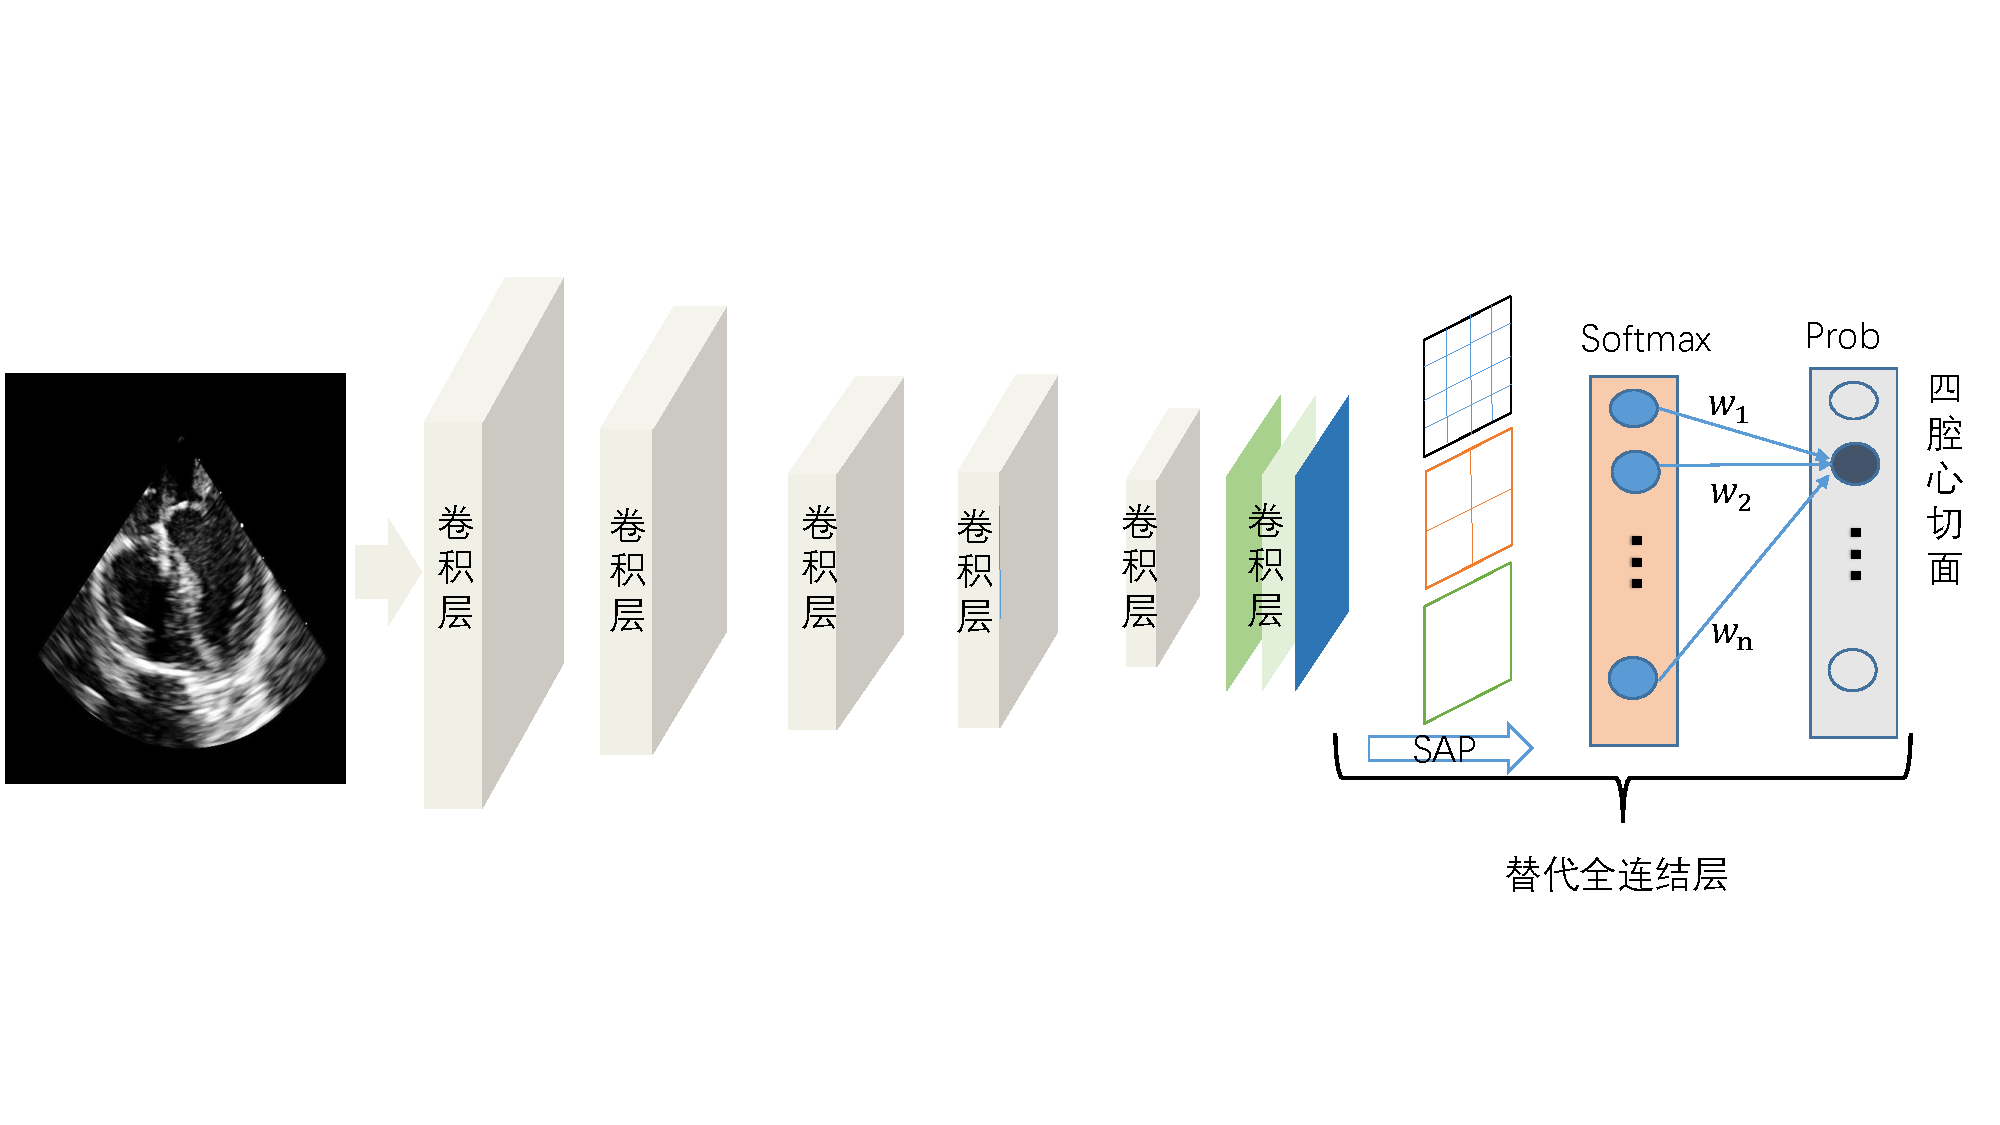
\includegraphics[trim = 30mm 0mm 30mm 0mm, clip, width=0.45\textwidth]{ch03_02}
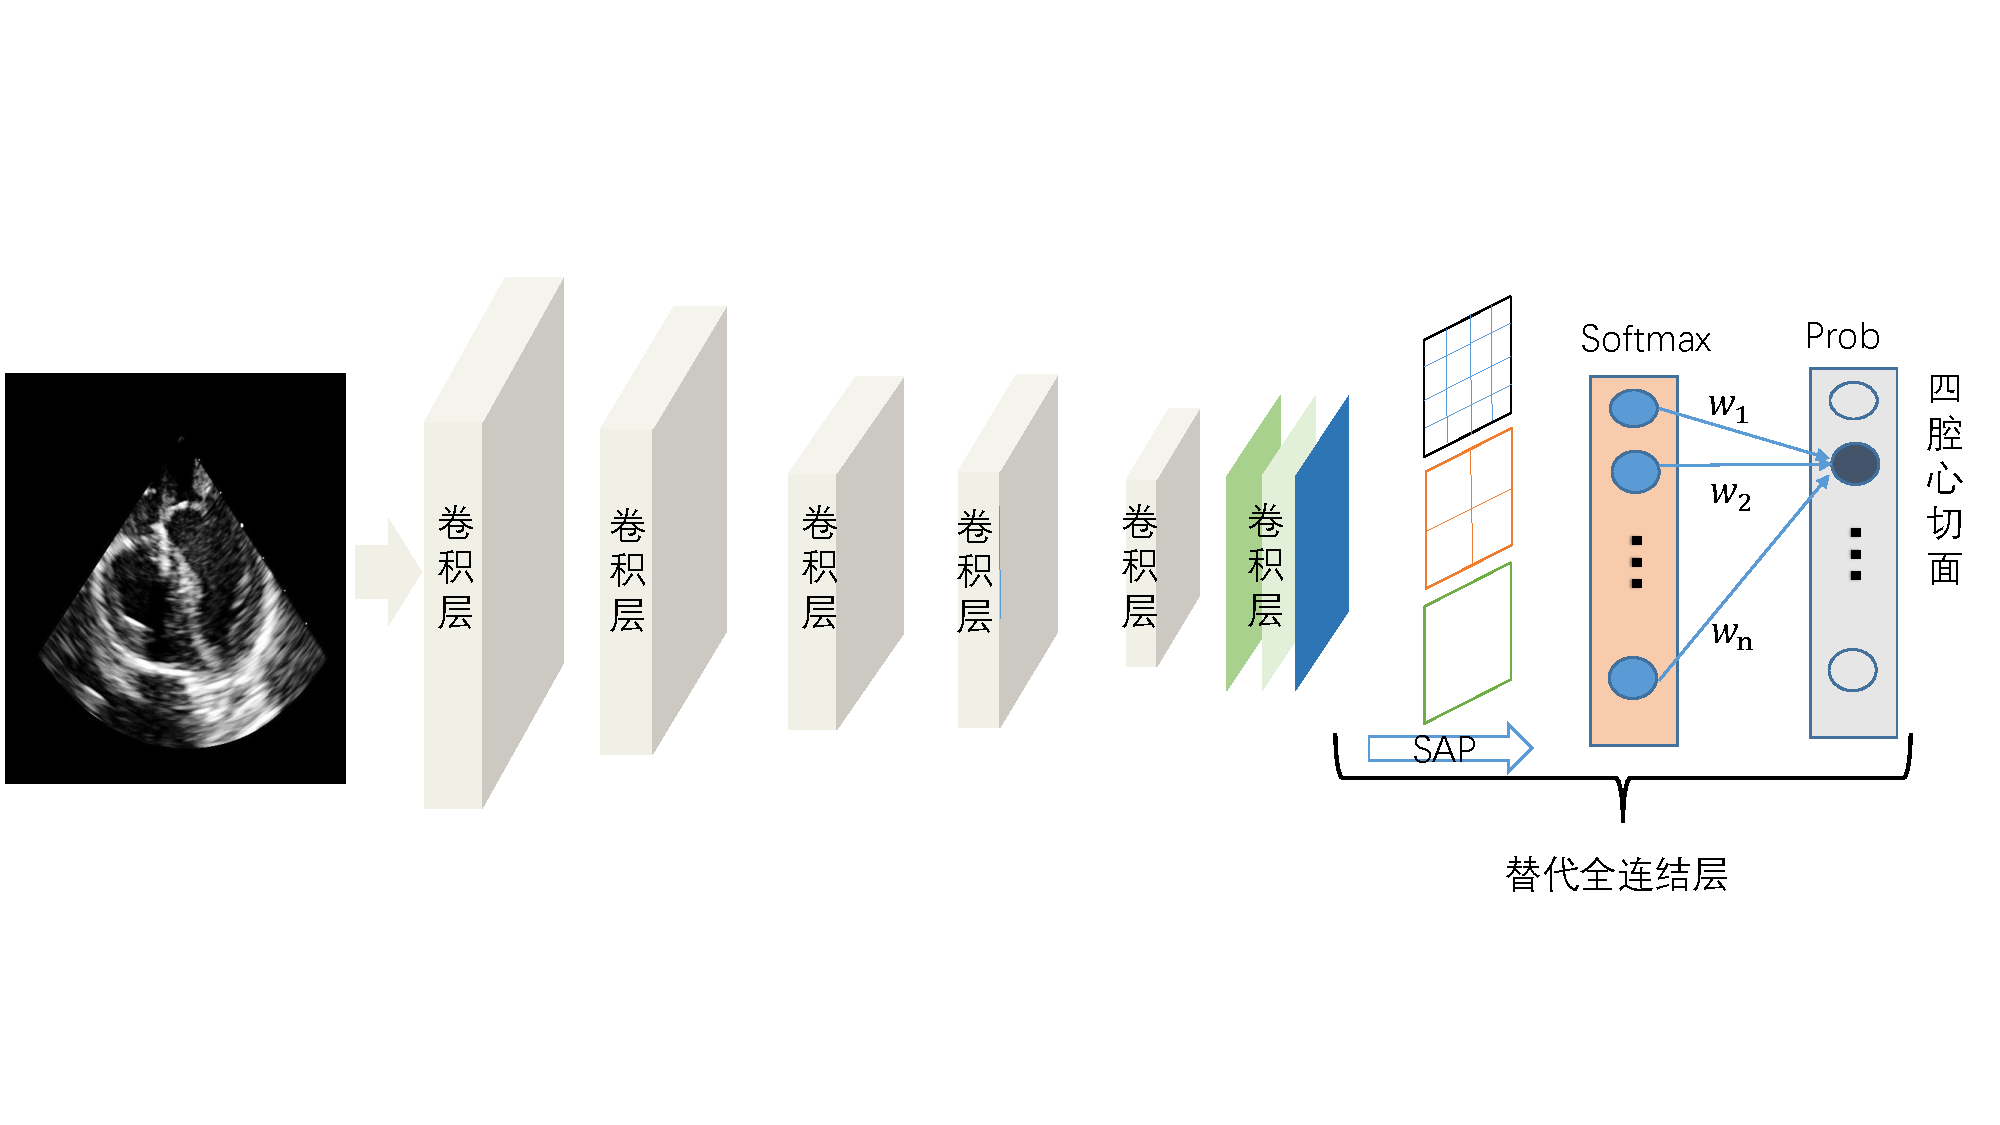
\includegraphics[width=0.9\textwidth,height=0.4\textheight]{ch03_02}
\caption{七类标准切面超声心动图及数量分布}
\label{fig:ch03_02}
\end{figure}

试验中所用标准切面类别和数量分如布图\ref{fig:ch03_02}所示。依据探头在食管中段(ME)和经胃底(TG)的位置和角度不同,在图\ref{fig:ch03_02}中7类标准切面分别为:a为升主动脉长轴(AescLAX) ,b为主动脉瓣长轴(MEAVLAX),c为主动脉瓣短轴(MEAVSAX),d为降主动脉长轴(descLAX),e为降主动脉短轴(descSAX),f为食管中段四腔心(ME4C),g为经胃底心室短轴(TGLAX)。其中,d,e,g为单扇形切面,其余为双扇形中截取的切面。训练集(17932张)和测试集(2217张)由不同时期采集不同病人对象数据的随机划分。值得注意的是,所有数据都经过裁剪操作以隐去患者信息。
\subsection{识别实验结果和分析}

本文在构建的超声心动图的数据集上测试分类性能。采用Caffe框架\citep{Jia2014}实现深度卷积网络结构,预训练模型来自Caffe model zoo。使用具有Intel®Core TM i5 3.2GHz处理器和12GB内存的Tian X GPU测量所需的时间,单个切面所需的分类识别时间平均需要10毫秒,基本可满足实时识别。

为验证从自然图像训练的模型能迁移到经食道超声心动图上,输入图像归一化为256x256,网络初始学习率设为0.001,迭代一定轮数动态调整学习率大小,其他参数的设置跟原文献中训练网络结构时一致。三种不同网络结构的深度模型微调前后在同一测试集上的准确率随着迭代次数的增加最后趋于一致,如表\ref{tab:ch03_01}所示,Scratch表示不经过微调,Finetune表示经过微调。Deep-echo模型结构跟AlexNet模型类似,是在其结构基础上去掉全连接层,用空间金字塔池化层代替,比VGG16和GoogLeNet模型的层数更少,模型结构更简单,而分类准确率却接近,表明提出方法的有效性。针对VGG16模型和Google Net模型也可同样设置,本文主要关注点不是得到分类精度最优的分类模型,故并未全部加以实验验证。
\begin{figure}[!htbp]
\centering
%trim option's parameter order: left bottom right top
%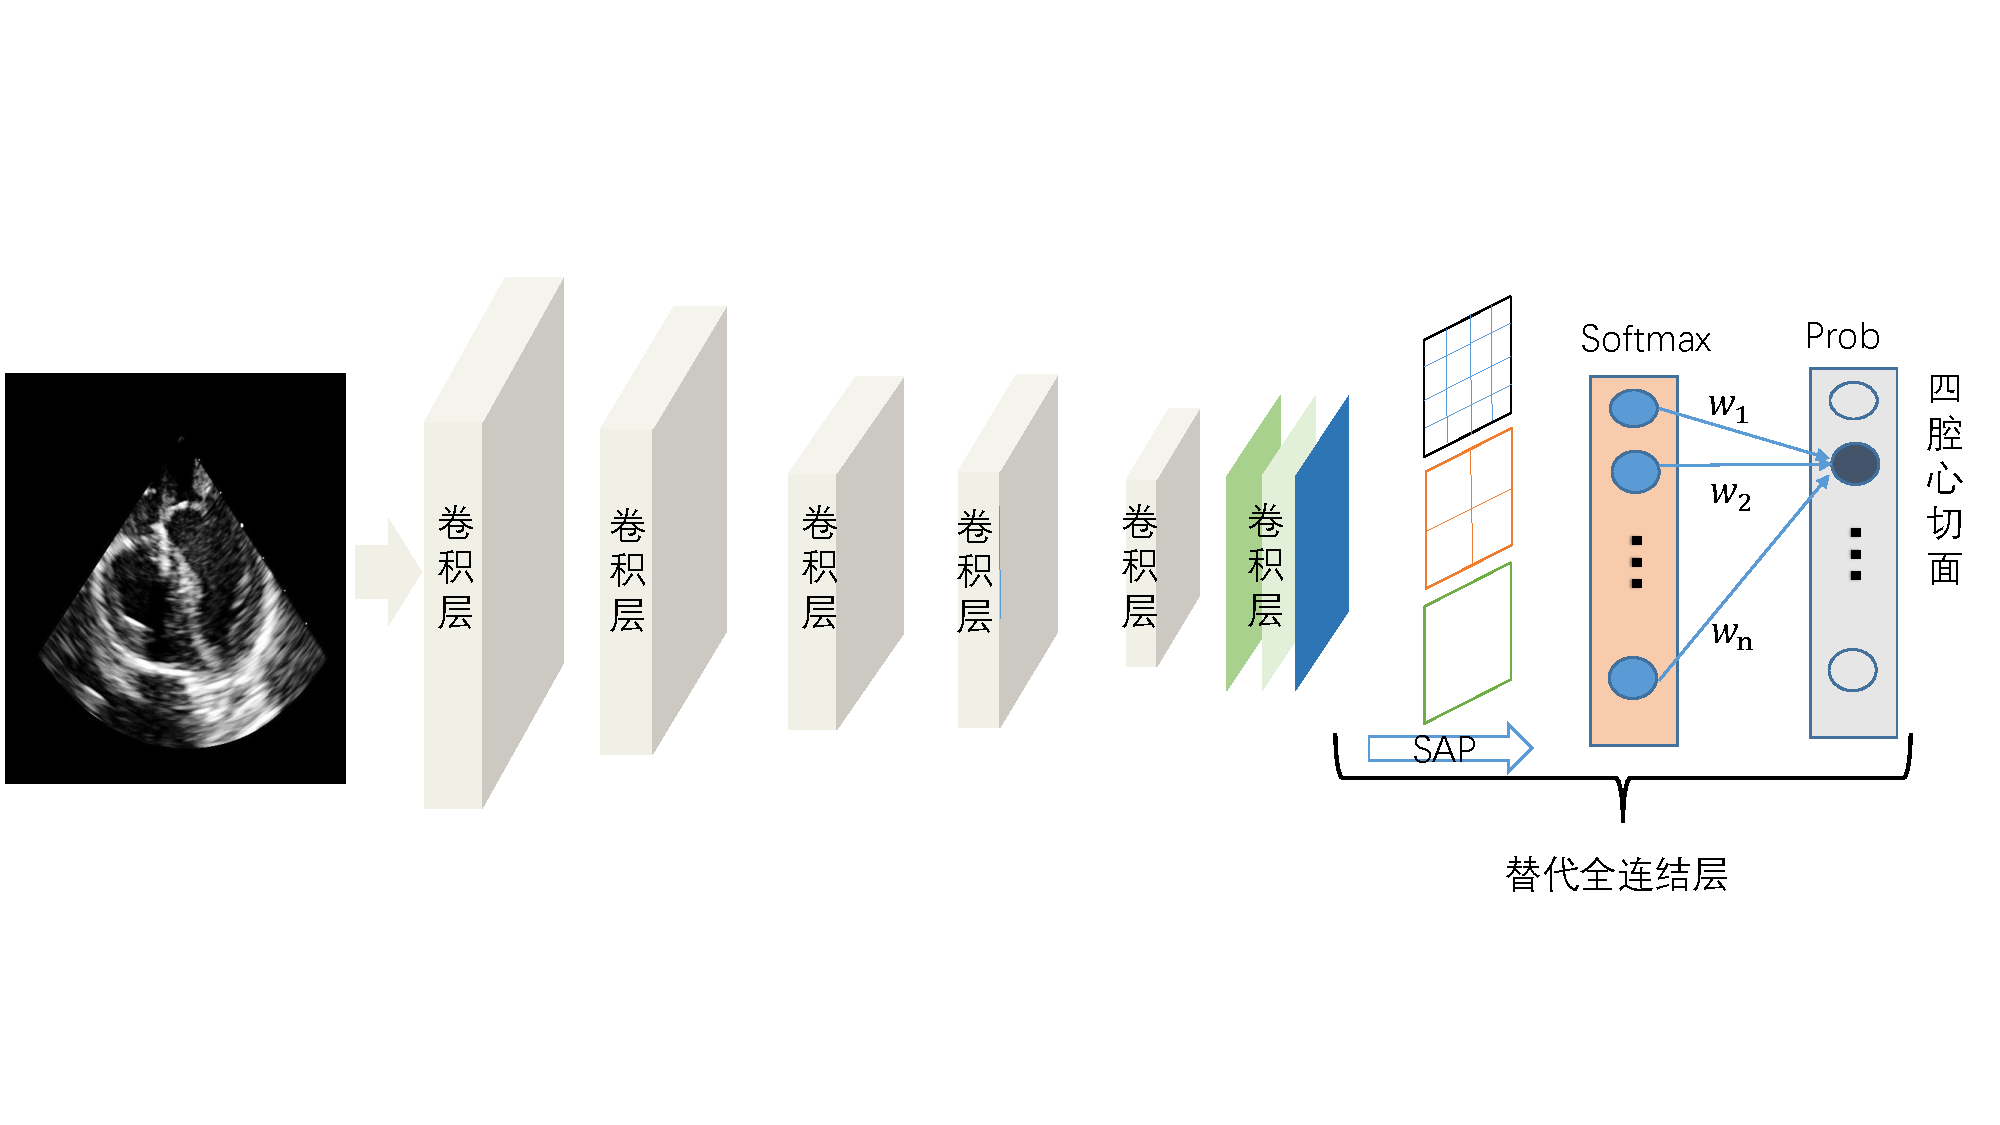
\includegraphics[trim = 30mm 0mm 30mm 0mm, clip, width=0.45\textwidth]{ch03_02}
\includegraphics[width=0.9\textwidth]{ch03_03}
\caption{Deep-Echo模型分类的混淆矩阵}
\label{fig:ch03_03}
\end{figure} 
\begin{figure}[!htbp]
    \centering
    %trim option's parameter order: left bottom right top
    %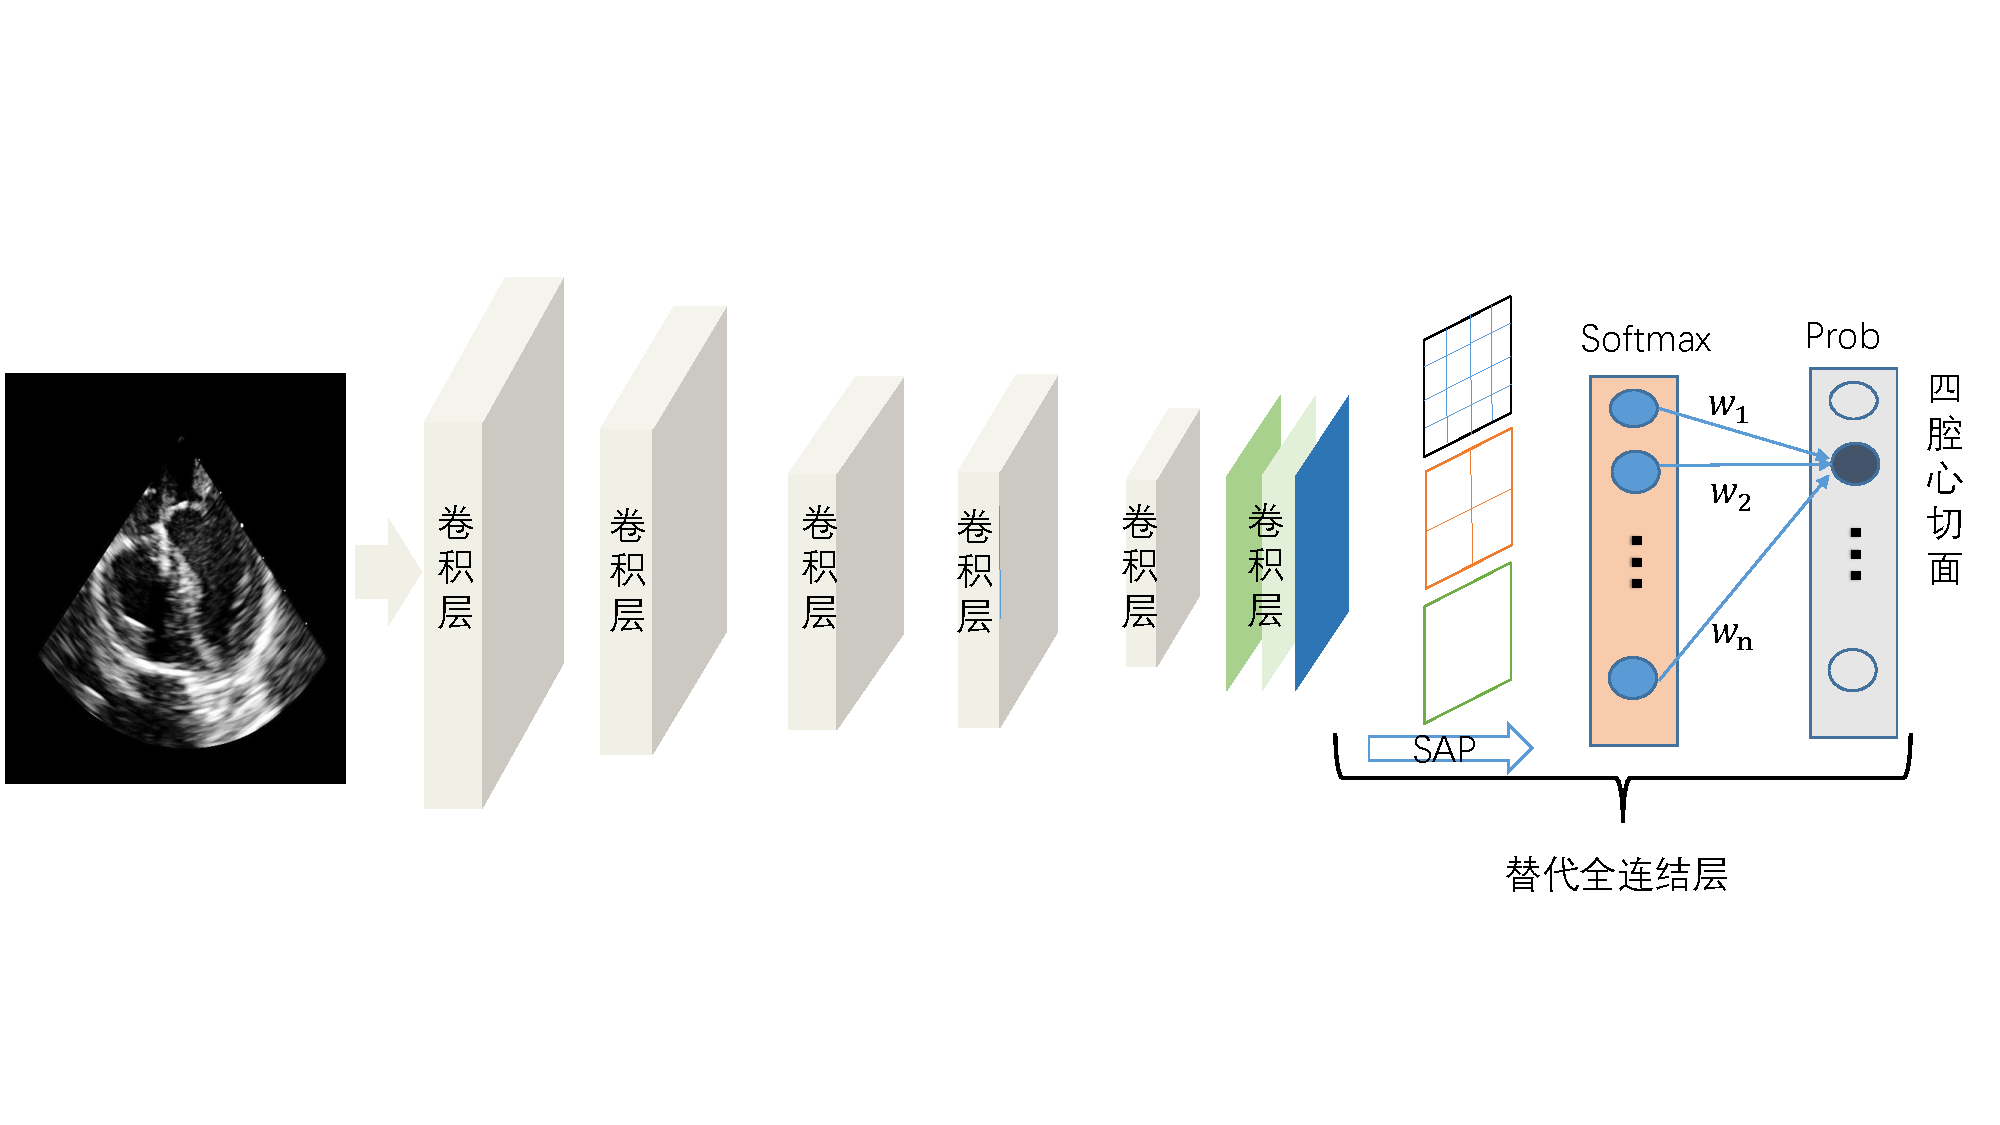
\includegraphics[trim = 30mm 0mm 30mm 0mm, clip, width=0.45\textwidth]{ch03_02}
    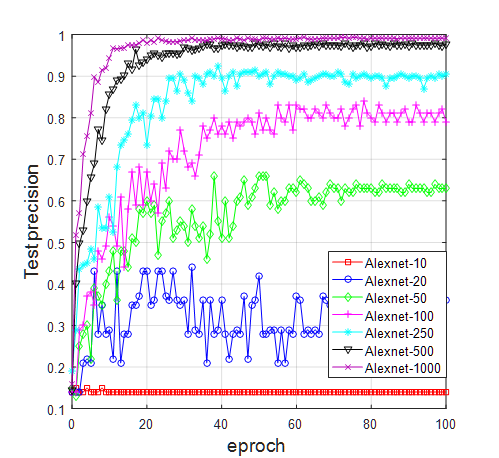
\includegraphics[height=20mm,width=0.9\textwidth]{ch03_04}
    \caption{不同数据量的平均分类精度}
    \label{fig:ch03_04}
    \end{figure} 
为验证训练集数据量对深度卷积网络的影响。网络结构采用AlexNet模型结合空间金字塔池化层,在不同数据量上微调,实验结果如图\ref{fig:ch03_04}所示,数字代表每类至多的数目,随着数据量的增加,模型准确率随之提升,可知针对超声心动图标准切面识别问题,并不用构建很大的数据集进行识别,如图\ref{fig:ch03_03}中每类至多500达到的平均准确率接近使用全部训练集的结果。可推断采用微调技术,能显著减少深度模型对大数据量的依赖。
\begin{table}[!htbp]
    \centering
    \footnotesize% fontsize
    \setlength{\tabcolsep}{4pt}% column separation
    \renewcommand{\arraystretch}{1.2}%row space 
    \begin{tabular}{lcccccccc}
        \hline\hline
          \multicolumn{2}{c}{\ \ \ \ \ \ \ \ \quad 平均分类精度比较} \\
        \cline{2-3}% partial hline from column i to column j
           \qquad  & Scratch & Finetune \\
        \hline
        AlexNet & $93.35\%$ & $93.68\%$ \\
        \hline
        VGG16 & $96.66\%$ & $96.81\%$ \\
        \hline
        GoogleNet & $97.36\%$ & $97.42\%$ \\
        \hline
        Deep-Echo & $\textbf{97.49\%}$ & $\textbf{99.12\%}$ \\
        \hline\hline
    \end{tabular}
    \caption{不同模型分类精度比较}
    \label{tab:ch03_01}
\end{table}

为了验证最优模型在不同类别的分类性能,7分类的混淆矩阵如图\ref{fig:ch03_04}所示,每行代表实际的类别标签,每列代表预测的标签。最终的平均分类精度为97.49\%。分类置信度较低的是升主动脉长轴(AescLAX),其他各类的准确率都较高。

\subsection{模型可解释性实验结果分析}
深度卷积网络能在标准切面识别问题上得到较高的分类精度,但仅从分类准确率上评价模型存在局限性。为分析模型的有效性,采用文中所述可视化方法,对迁移后的Deep-echo模型进行实验。
\begin{figure}[!htbp]
\centering
%trim option's parameter order: left bottom right top
%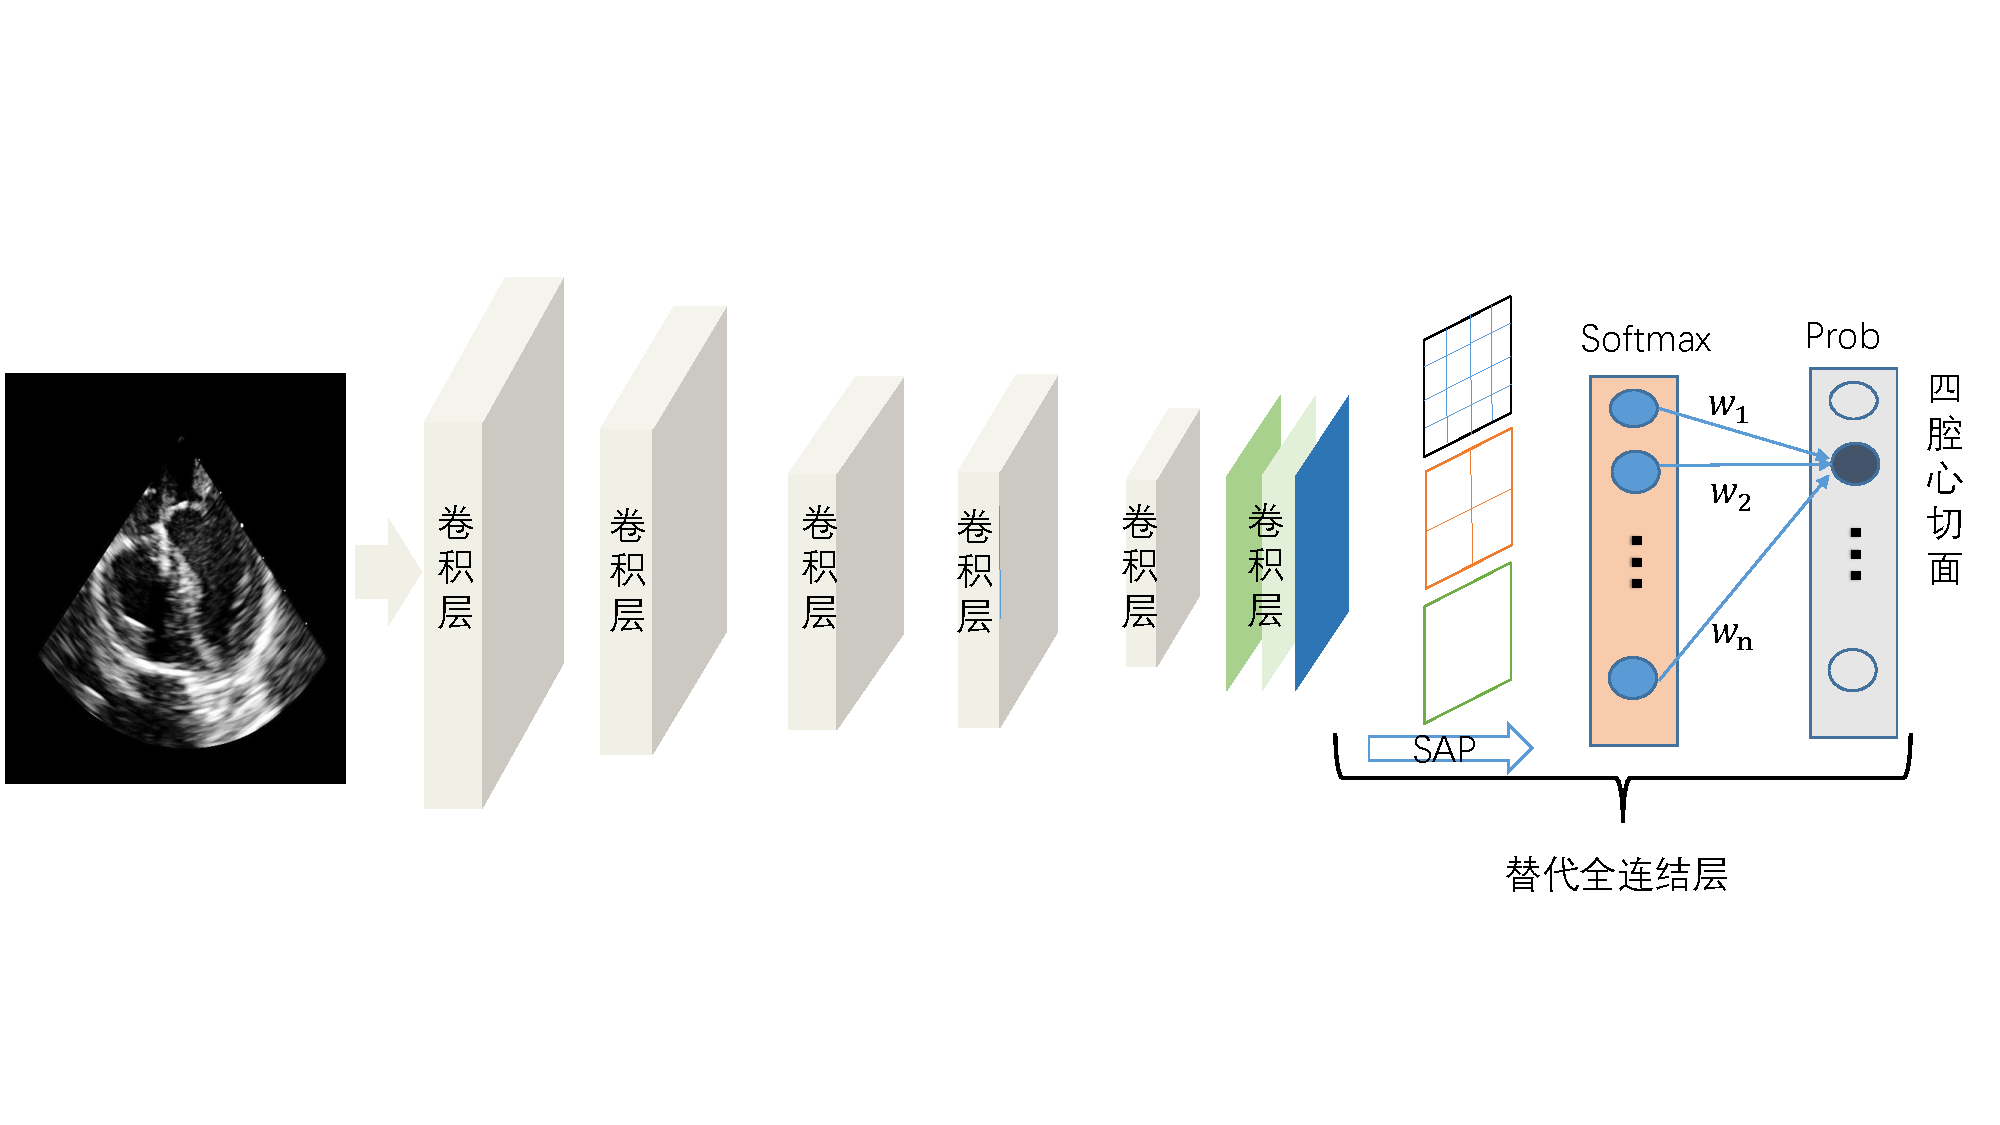
\includegraphics[scale=0.6,trim = 30mm 0mm 30mm 0mm, clip, width=0.45\textwidth]{ch03_02}
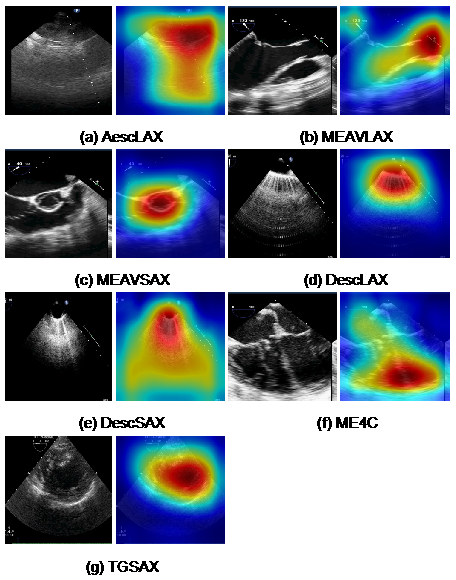
\includegraphics[height=60mm,width=0.9\textwidth]{ch03_05}
\caption{各类切面的原图和显著性热力图}
\label{fig:ch03_05}
\end{figure}  
实验结果如图\ref{fig:ch03_05}各类切面的原图和显著性热力图所示,图中为各类切面和对应的类别显著性热力图。类别显著性图中的颜色从蓝到红,表示原图像素中对分类结果影响的重要性是从轻到重。图中结果能很好的解释模型的有效性,并且跟专业医师的判断一致,如图\ref{fig:ch03_05}c中显著性热力图红色区域图定位到图中的圆圈;图\ref{fig:ch03_05}d中定位到的干涉条纹;图\ref{fig:ch03_05}f定位到左心室和右心室的边界等;都跟医师的决策判断依据是一致的。
\begin{figure}[!htbp]
\centering
%trim option's parameter order: left bottom right top
%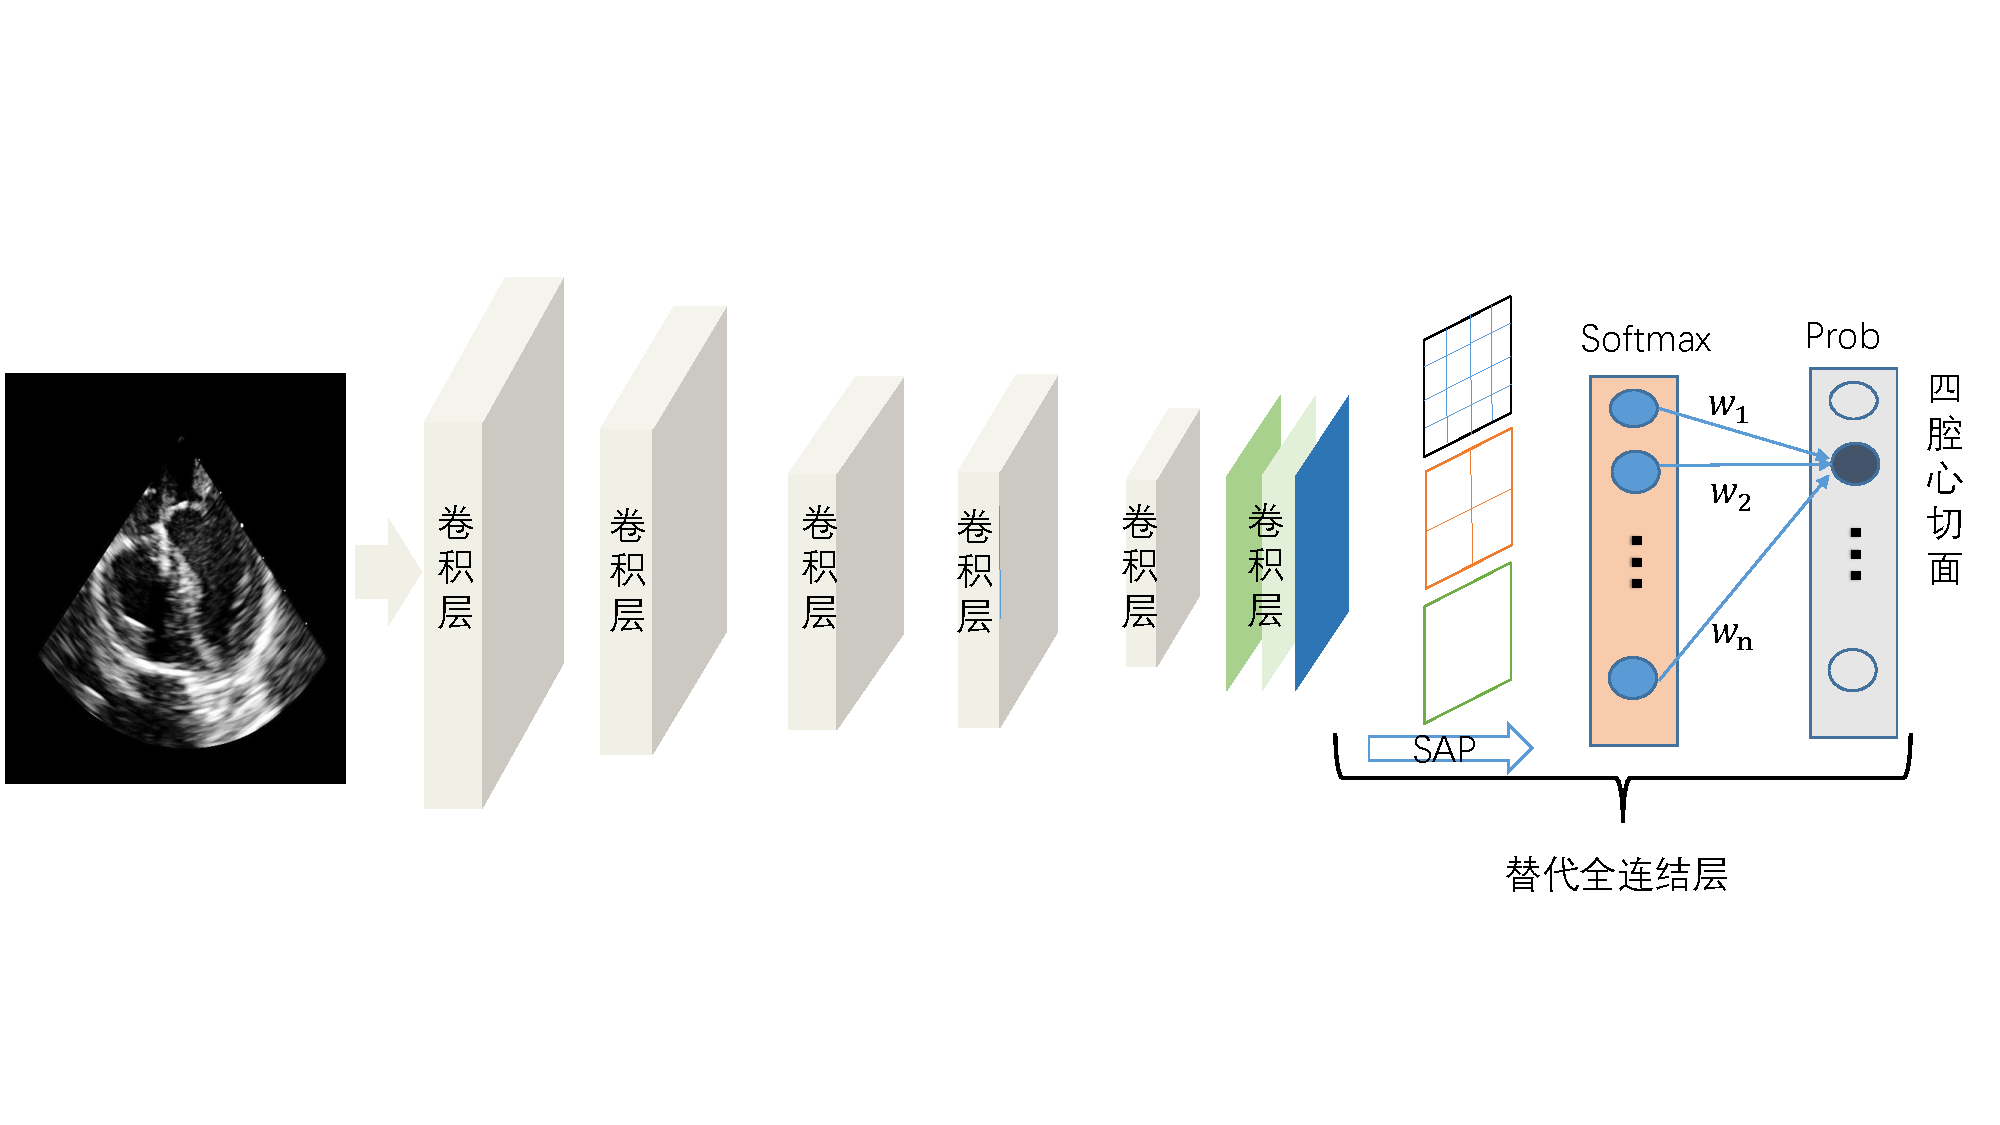
\includegraphics[scale=0.6,trim = 30mm 0mm 30mm 0mm, clip, width=0.45\textwidth]{ch03_02}
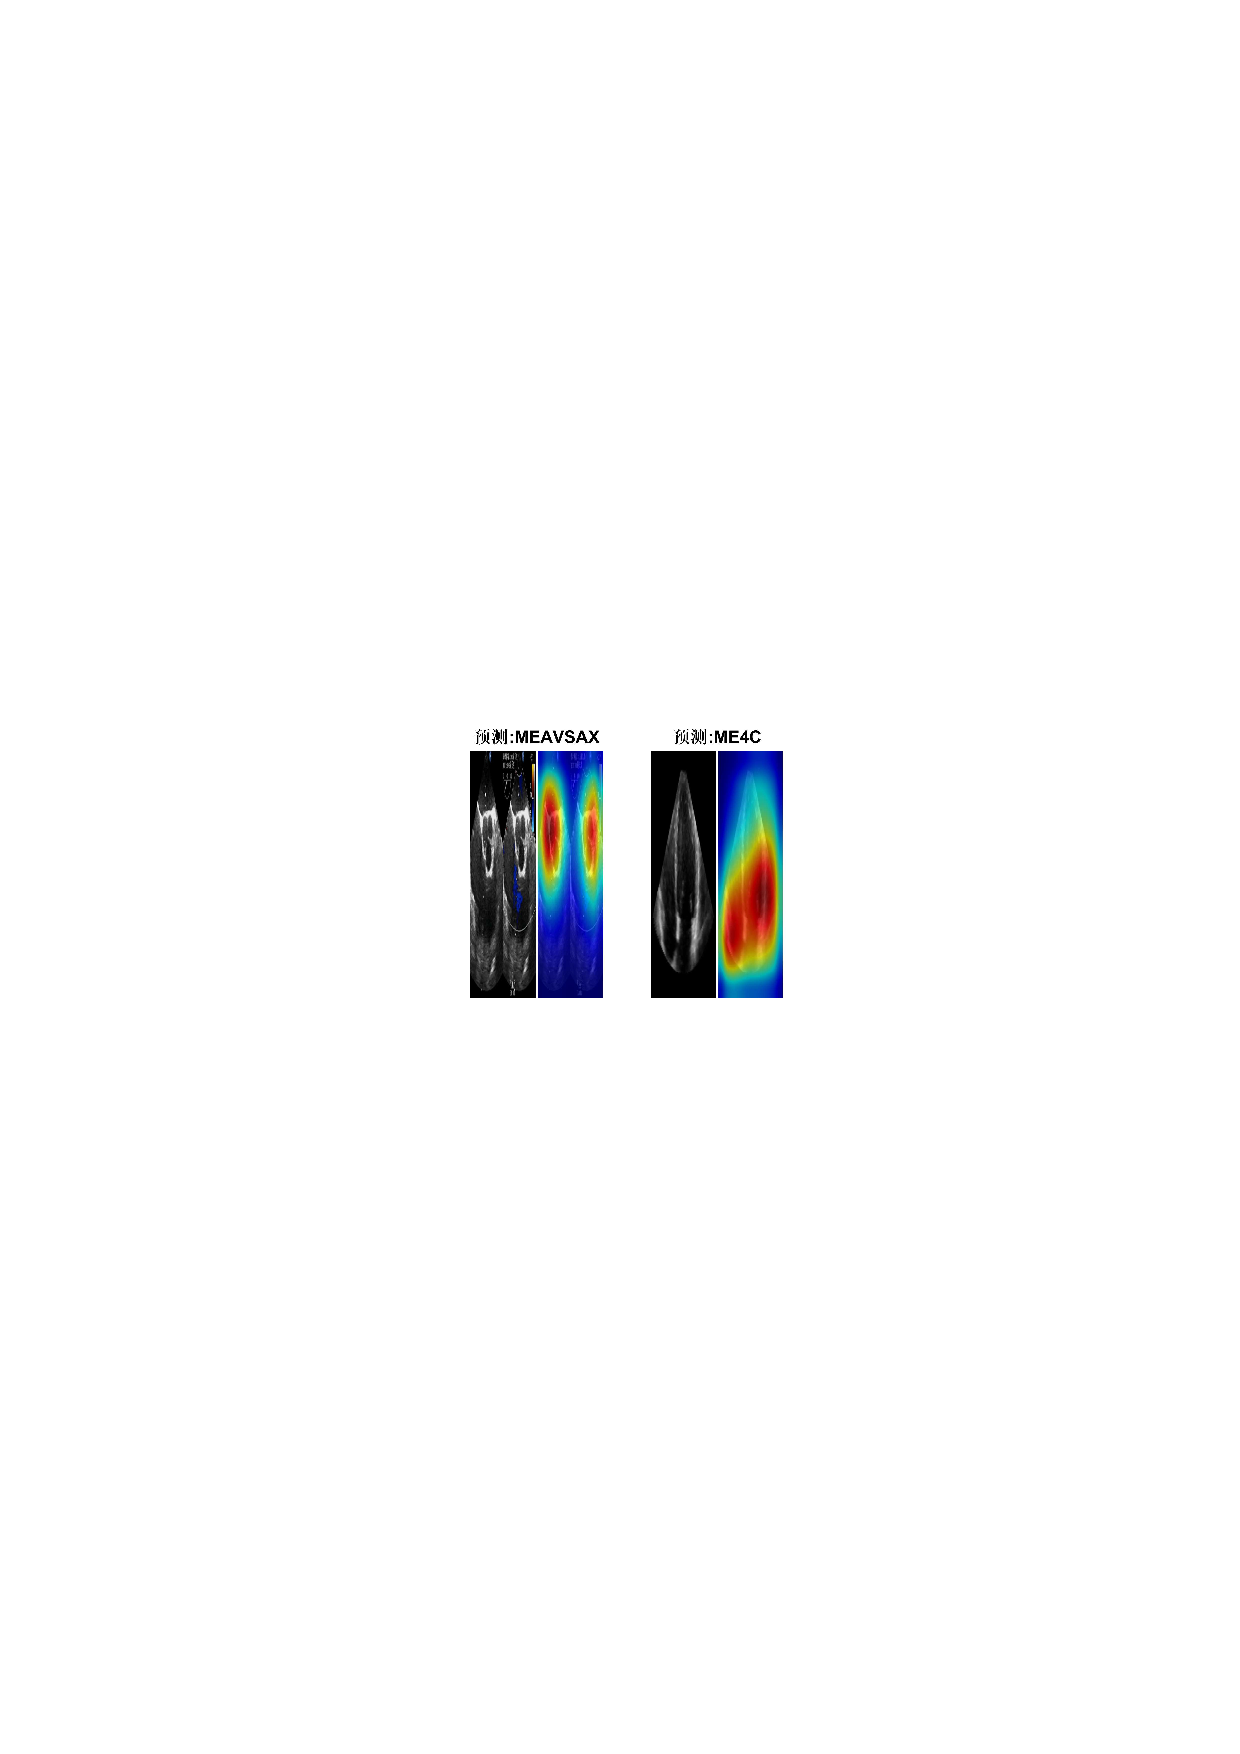
\includegraphics[width=0.9\textwidth,height=0.15\textheight]{ch03_06}
\caption{深度模型泛化性能可视化分析}
\label{fig:ch03_06}
\end{figure}    
深度模型泛化性能可视化结果如图\ref{fig:ch03_06}所示,原图像分别是带彩色多普勒的双扇形切面(图\ref{fig:ch03_06}a)和经胸的四腔心切面(图\ref{fig:ch03_06}b),这两个图是跟数据集中的经食道超声心动图差异较大,说明深度卷积网络模型确实能对标准切面进行语义分类,表明模型确实能提取到高层语义的特征,深度卷积网络泛化能力优异。
可视化结果也能很好的解释模型的有效性,如图\ref{fig:ch03_06}中显著性热力图红色区域图定位到图中的圆圈,也是医师认定该切面的关键性结构,图\ref{fig:ch03_06}b定位到左心室和右心室的边界等,都跟医师的决策判断依据是一致的。并且该方法也能作为判断学习模型是否有效的根据,不经过微调的模型虽然能得到较高的分类准确度,并不能得到类似的显著性热力图。

\section{小结与讨论}
本章针对深度特征表示的高层语义在医学图像的具体应用——超声心动图标准切面的自动识别,本文提出了一种基于深度卷积神经网络的超声心动图标准切面自动识别方法,利用所述全局空间金字塔均值池化方法进行微调迁移学习,实验结果表明该方法识别准确率高,并实验分析了数据规模对模型分类精度的影响,结果表明基于深度卷积网络的识别方法应成为超声心动图自动识别的基准方法,接下来会探索更精细类别分类问题,如舒张末期和收缩末期标准切面的识别等。可视化深度模型的实验,对模型的可解释性和有效性进行了分析,推断深度模型的优异的分类性能和泛化能力的原因是可以对类别显著性区域进行判别,采用的可视化方法是对网络模型整体的理解,具体各层特征怎么耦合成语义信息仍需进一步探索。本章研究内容和主要成果以题为《基于深度学习的超声心动图切面识别方法研究》的论文形式已发表在学术期刊上\citep{tao2017}。






\chapter{空间金字塔分解的深度可视化方法}
\label{chap:visualization}

以深度卷积神经网络(Convolutional Neural Network,CNN)为代表的深度学习对计算机视觉和机器学习领域产生了深远影响。但是完全理解深度学习模型的内在工作原理,设计高性能的深度网络结构还是很困难的,一直以来人们普遍将其内部工作原理看成一个“黑箱”,这是由于深度CNN存在海量参数,多次迭代更新生成输入输出之间相当不连续和非线性的映射函数;以及对参数的初始状态敏感,存在很多局部最优点。探究CNN的运行机制,核心在于它究竟自动提取什么样的特征,经过卷积层、池化层,特征都是分布式表达的,每个特征反映在原图上都会有重叠,故希望建立特征图与原图像之间的联系,即深度可视化。该技术试图寻找深度模型所提取各层特征较好的定性解释,并在设计开发新网络结构方面扮演重要角色。


目前针对CNN可视化的研究,主要集中在如何理解CNN从海量数据中自动学习到的,能反映图像本质的分层特征表达,即获得网络中隐藏层神经元与人类可解释性概念之间的联系。最直接的方法是展示学习得到的卷积核和相应的特征图,但除了首层卷积核和特征图有直观的解释外,其余各层并没有可解释性。从信号处理的角度看,基于CNN高层特征的分类器在输入域,需要较大感知野,才能对以由低频为主的输入图像进行多层非线性响应,并对小的输入改变产生平滑不变输出。同时,由于经过非线性激活函数变换和池化,引入空间不变性获得更好识别性能的同时,也对可视化带来新的挑战。


深度可视化技术可以简单分为三类:基于梯度更新的方法\citep{Erhan2009,simonyan14deep,Lenc2015,Szegedy2013a,JasonYosinski2015,Nguyen2016a,Nguyen2016b};基于特征重建的方法\citep{Zeiler2014,Brox,Mahendran2015d,Mahendran2015}];基于相关性的方法\citep{Cao2015,Bach2016}。基于网络梯度更新的思想是由Erhan等\citep{Erhan2009}引入,固定模型参数通过梯度更新改变输入值,最大化激活单一神经元或标签类别概率。激活最大化生成的非自然图像还可以是网络模型的对抗样本\citep{Goodfellow2014}。Simonyan等\citep{simonyan14deep,Lenc2015,Szegedy2013a}通过梯度上升方法迭代寻找使得最大化激活CNN某个或某些特定的神经元的最优图像,其假设神经元对像素的梯度描述了当前像素的改变能影响分类结果的强度。文献\citepns{simonyan14deep}引入L2正则化先验(或称权重衰减),改进可视化效果。Yosinski等\citep{JasonYosinski2015}进一步提出高斯模糊正则化、梯度剪切等技术,其中梯度剪切指的是每次只更新对分类最有利的一部分梯度,改善生成图像质量。文献\citepns{Lenc2015,Nguyen2016b}考虑神经元的多面性和利用生成网络作为自然图像的先验来合成更自然的图像。

Zeiler等\citep{Zeiler2014}提出利用反卷积网络,利用反向传播重构各层特征到像素空间的映射,并用于指导设计调优网络结构,提高分类识别精度。在反卷积过程中利用翻转原卷积核近似作为反卷积核,针对特定特征图在训练集上重新训练。
Dosovitskiy等\citep{Brox}提出通过学习‘上’卷积网络来重建CNN各层的特征,指出结合强先验,即使用于分类的高层激活特征也包含颜色和轮廓信息。Mahendran等\citep{Mahendran2015d,Mahendran2015}通过对学习到的每层特征表达进行反编码重建,提出利用全变分正则化和自然图像先验,并将L2范数正则化推广到p范数正则化,得到较优的可视化效果。


本文主要关注前两种方法中的正则化技术,基于相关性分解方法请参考文献\citepns{Bach2016}。受文献\citep{Huang2017c,Denton2015}启发,把用于图像生成的拉普拉斯金字塔,进一步扩展成空间金字塔分解方法,并引入显著性激活图技术进一步改进深度CNN的可视化效果。
\section{可视化方法的数学模型}

激活最大化和特征表达反编码重建均是针对已经训练好的模型,对给定输入$x_{i}\in R^{C\times H\times W}$,其中C为颜色通道数,H,W为图像高和宽。CNN模型可抽象为函数$\phi$:$R^{C\times H\times W}\rightarrow R^d$,其第i个神经元的激活值为$\phi _{i}(x)$,对给定图像$x_{0}$ 的特征编码$\phi _{0}=\phi (x_{0})$,定义参数$\theta$ 的正则化项$R_{\theta}(x)$,寻找使得能量泛函最小化的初始输入$x^*$,其数学模型为
\begin{equation} 
\label{eq:ch04_01}
     x^*=\underset{x}{argmin} (l(\phi (x),\phi _{0})) + \lambda R_\theta(x))
\end{equation}

其中, $l$损失比较的是$\phi (x)$ 和目标$\phi_{0}$ 的差异,选择不同的损失函数定义不同的可视化方法。但该优化通常是一个非凸优化问题,通常采用梯度下降法去寻找局部最优值为
\begin{equation}
\label{eq:ch04_02}
     x \leftarrow x+ \alpha \frac{\partial \phi _{i}(x)}{\partial x}
\end{equation}
激活最大化方法是文献\citepns{Erhan2009}中提出针对深度架构中任意层中的任意神经元所提取的特征,寻找使一个给定的隐含层单元的响应值$\phi _{0}\in R^d$ 最大的输入模式,可由内积形式定义$l$ 损失为
\begin{equation} 
\label{eq:ch04_03}
     l(\phi (x),\phi_{0}) =-<\phi (x),\phi _{0}>
\end{equation}
  式中$\phi_{0}$ 需人工指定,最大化激活的目标可以是全连接层的特征向量,也可以是卷积层某一通道的某一神经元的激活值。
特征表达的反编码重建,通过最小化给定特征向量与重建目标图像特征向量间的 损失,一般采用欧式距离来衡量损失误差,定义如下 
\begin{equation} \label{eq:ch04_04}
     l(\phi (x),\phi _{0}) = \frac{\parallel\phi (x)-\phi _{0} \parallel^2 }{\parallel \phi _{0} \parallel^2 }
\end{equation} 
但也可利用其它距离度量函数来评价损失。

\section{梯度更新的可视化方法}
 
用于分类的深度CNN提取高层语义信息的同时,丢失了大量低层结构信息。由于首层卷积核大都类似Gabor滤波器,导致梯度更新可视化生成图像中包含许多高频信息,虽然能产生大的响应激活值,但对可视化来说导致生成的图像是不自然的。还由于网络模型的线性操作(如卷积)导致对抗样本\citep{Goodfellow2014}的存在,为得到更类似真实自然图像的可视化结果,需在优化目标函数中引入正则化作为先验。
\subsection{$p$ 范数正则化方法} 

对图像来说,像素大小需在一定范围内,直接最大化激活类别概率,生成图像类似随机噪声图像。文献\citepns{simonyan14deep}通常引入L2范数正则化,惩罚过大和过小的极端值,其公式为$R_{\theta}(x)=\parallel x \parallel _{2}^{2}$。在文献\citep{Mahendran2015}中将其扩展到彩色图像RGB通道空间中的$p$范数正则化为
\begin{equation} \label{eq:ch04_05}
       R_{\theta}(x)= \frac{1}{HWC^p}\sum_{h=1}^{H}\sum_{w=1}^{W}(\sum_{c=1}^{C}x(x,w,c)^2)^{\frac{p}{2}}
\end{equation}
式中h,w表示图像的行和列大小,c表示颜色通道数,对比发现,文献\citepns{simonyan14deep}提出的L2正则化是忽视各颜色通道的差异的,正则化的力度可通过缩放常量p进行控制,即使得图像像素值大小保持在合适的范围内。
\subsection{高斯模糊和TV变分}

基于梯度更新可视化方法,引入高斯滤波器主动惩罚高频信息\citep{JasonYosinski2015},高斯模糊核半径大小由高斯函数的标准差控制,可随迭代次数动态调整模糊核大小。

全变分\citep{Mahendran2015}(Total Variance,TV)跟高斯模糊类似,鼓励可视化生成分片的常量块区域,对离散图像全变分操作可由有限差分来近似求解为    \begin{equation} \label{eq:ch04_06}
       R_{TV}(x)= \frac{1}{HWC^\beta}\sum _{hwc}((x(h,w+1,c)-x(h,w,c))^2+(x(h+1,w,c)-x(h,w,c))^2)^{\frac{\beta}{2}}
\end{equation}
式中 $\beta =1$,但其在可视化过程中,在图像的平坦区域并不存在边缘,全变分操作仍沿着边缘方向扩散就会导致出现虚假的边缘,会引入所谓的“阶梯效应”现象。$\beta<1$时结合超拉普拉斯先验\citep{Krishnan2009}能更好匹配自然图像的梯度统计分布,但对可视化来说反而使得可视化更困难。文献\citepns{Mahendran2015}实际实验表明,跟高斯模糊核一样,需随迭代次数动态调整$\beta$ 大小。
\subsection{基于数据统计先验}

	由于常规可视化方法并没有对颜色分布进行建模,文献\citep{Lenc2015}提出通过引入外部自然图像数据,计算图像色块先验为
\begin{equation} \label{eq:ch04_07}
       R_{\theta}(x)= \sum_{p}\parallel x_{p}-D_{p}\parallel _{2}^{2}
\end{equation}
式中$p$为块索引,$x_{p}$ 表示稠密采样的归一化图像块, $D_{p}$表示自然图像块数据库中距离$x_{p}$ 最近图像块。该方法跟文献\citep{Huang2017c}中利用参考图像“指导”人脸图像嵌入重建类似。并且基于数据的统计先验可进一步扩展,引入生成对抗网络,利用生成网络主动生成自然图像先验\citep{Nguyen2016a}。

 
 
\section{空间金字塔分解}
 
前文介绍的正则化先验主动限制图像空间中高频率和高振幅信息,生成的可视化图像存在如下问题:1)彩色图像的颜色分布仍是不自然的。2)生成的图像中包含可识别类别对象的多个重复成分,并且这些部件不能组合成完整的有意义整体。3)缺乏令人可信的低频细节,存在棋盘效应,只是形似。针对这些问题提出利用空间金字塔分解,主动提升低频信息和调控高频信息以改善生成图像的可视化效果。

\subsection{高斯和拉普拉斯金字塔分解}
 
拉普拉斯金字塔(Laplacian Pyramid,LP)\citep{Burt1983}是由一系列包含带通滤波器在尺度可变的图像上加低频残差组成的。首先通过高斯平滑和亚采样获得多尺度图像,即第K层图像通过高斯模糊、下采样就可获得K+1层,反复迭代多次构建高斯金字塔(Gaussian Pyramid,GP)。用高斯金字塔的K层图像减去其第K+1层图像上采样并高斯卷积之后的预测图像,得到一系列的差值图像即为拉普拉斯金字塔分解图像。
拉普拉斯金字塔分解过程(见图1所示)包括4个步骤: 1)高斯平滑 ;2)降采样(减小尺寸); 3)上采样并高斯卷积(图中expand操作); 4)带通滤波(图像相减) 。拉普拉斯金字塔突出图像中的低频分量,拉普拉斯金字塔分解的目的是将源图像分解到不同的空间频带上。
\begin{figure}[!htbp]
\centering
%trim option's parameter order: left bottom right top
%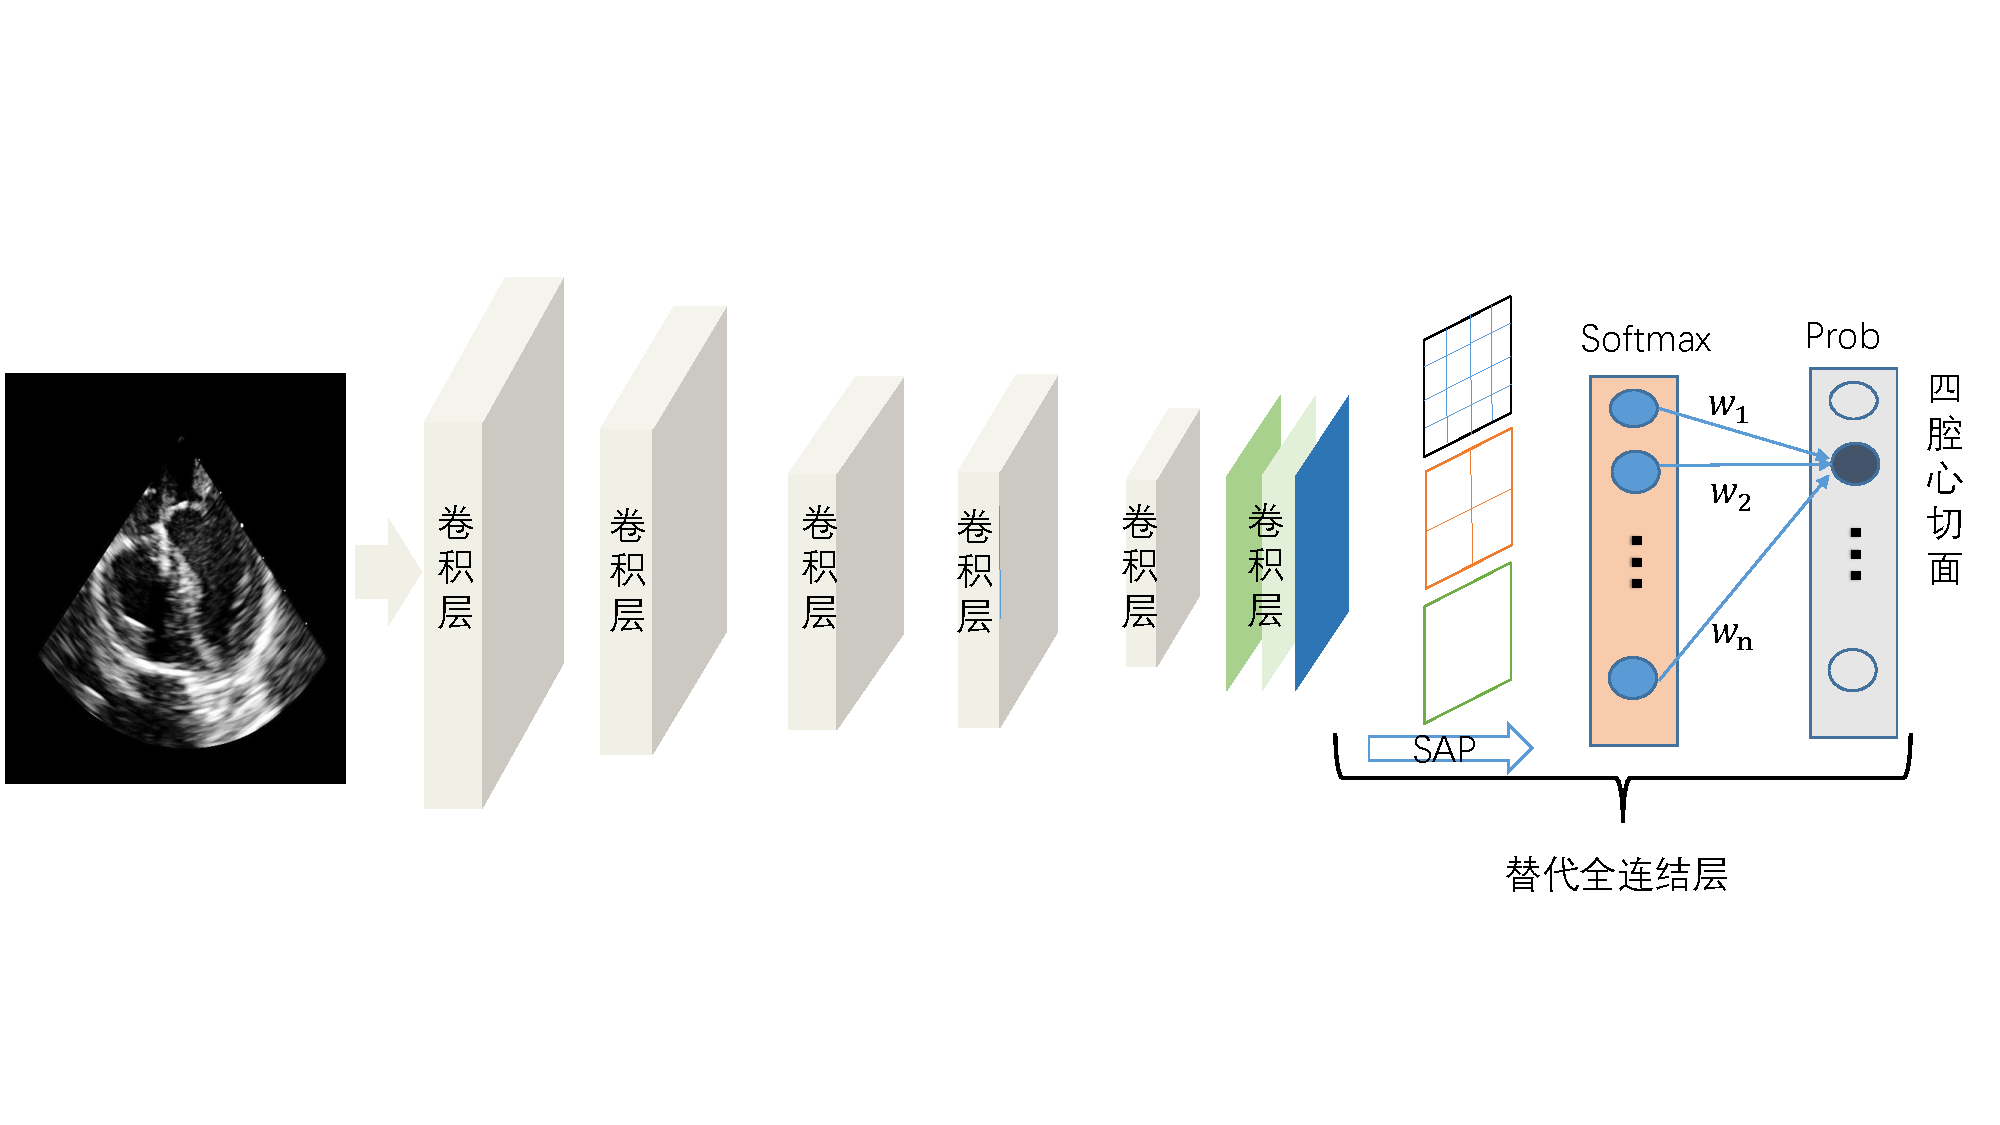
\includegraphics[trim = 30mm 0mm 30mm 0mm, clip, width=0.45\textwidth]{ch03_02}
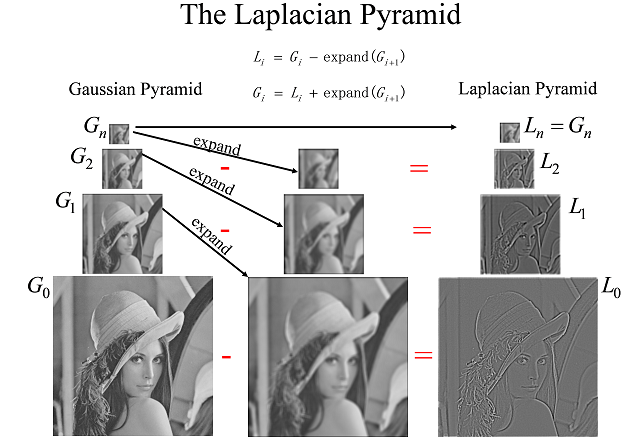
\includegraphics[width=0.85\textwidth]{ch04_01}
\caption{高斯和拉普拉斯金字塔}
\label{fig:ch04_01}
\end{figure}

由于自然图像统计特性中的尺度不变性,也称为$1/f$法则\citep{VanderSchaaf1996a},即自然图像集$I(f_{x},f_{y})$ 的平均傅里叶功谱服从$I~(f_{x},f_{y})^2$。在激活最大化可视化深度CNN模型过程中利用提出的高斯和拉普拉斯空间金字塔分解,调整生成梯度图像包含的频谱分量大小。其中空间金字塔分解正则化项为

\begin{equation} \label{eq:ch04_08}
       r_{\theta}(x)= \sum_{k=1}^{K}[LP_{k}+GP_{k}]
\end{equation}

式中k代表构建$k$层金字塔分解,本文实验$k$选取为4。$LP_{k}$为第$k$层的拉普拉斯金字塔分量,$GP_{k}$ 为第$k$层的高斯金字塔分量。


\subsection{梯度归一化}
  
	基于梯度更新的可视化方法,由于原输入空间中高低频分量混杂在一起,对原输入图像相应的更新梯度进行归一化操作能得到较好可视化效果,即对输入图像每次迭代更新的梯度,则提出梯度归一化操作:   
\begin{equation} \label{eq:ch04_09}
       g \rightarrow \frac{g}{g.std()+\delta}
\end{equation} 
式中 $\delta$为非负小常量,std表示梯度矩阵的方差。该梯度中心归一化技术,可以减少产生重复的对象碎片的倾向,而倾向于产生一个相对完整对象。梯度归一化的引入同批归一化(Batch Normalization)思想类似,校正CNN网络非线性变换引起的“偏移”,该方法也侧面验证最新提出的分层归一化\citep{Ioffe2014Batch}的有效性。
\subsection{类别激活图限制可视化区域}
根据文献\citepns{Zhou2015}提出的类别激活图技术,假设$f_{j}(x,y)$  表示最后的卷积层空间$(x,y)$位置上第$j$ 个神经元的激活值,则对$j$ 神经元的全局平均池化操作结果对给定类别$k$的得分函数$S_{k}$:
\begin{equation} \label{eq:ch04_10}
      S_{k}=\sum _{j} w_{j}^{k} \sum _{x,y}f_{j}(x,y)
\end{equation}
式中 $w_{j}^{k}$ 是第$j$ 个神经元和第 k类的连接权重。根据文献\citepns{Zhou2015},由式\ref{eq:ch04_10} 可得定义类别激活图$M_{k}$ 为	
\begin{equation} \label{eq:ch04_11}
      M_{k}=\sum _{j} w_{j}^{k}f_{j}(x,y)
\end{equation}
式中$M_{k}$ 表明在空间(x,y)位置的激活值对分类结果影响的重要性。对类别激活映射图直接双线性插值得到与原输入图像大小相等的显著性图。本文利用显著性激活图作为梯度更新的权重因子,即输入变为原始输入图像与类别激活图的加权乘积。动机是要求网络梯度更新保持在类别显著性区域内,压制无关背景信息的生成。具体详情请参见第四章实验部分。
\subsection{优化方法}

深度CNN模型优化策略的核心是随机梯度下降法,常用方法是带动量的随机梯度下降法为:
\begin{equation} \label{eq:ch04_12}
      V_{t}=\mu V_{t-1} -\alpha *\bigtriangledown {f(x_{i})}
\end{equation}          
\begin{equation} \label{eq:ch04_13}
     x_{t+1}=x_{t}+V_{t}
\end{equation}       
式中$\mu$ 为动量因子表示保持原更新方向的大小,一般选取0.9, $x_{t}$为在t时刻待更新的梯度,$\alpha$ 为学习率;文献\citep{Mahendran2015d,Mahendran2015} 采用自适应梯度(Adaptive Gradient,AdaGrad)\citep{Duchi2011}的变种算法,根据历史梯度信息自适应调整学习率。同时文献\citepns{Gatys2015a}采用的二阶优化算法针对纹理和艺术风格重建问题,得到比用基于一阶随机梯度下降算法更优的可视化效果。但本文通过实验对比发现对各种优化方法对生成图像质量影响不大,从简选择带动量的随机梯度优化方法。
\section{实验结果分析和讨论}
 
基于梯度更新的可视化方法主要用于激活最大化和特征重建,但文献\citepns{He2016}指出用随机未训练的CNN模型也能较好重建原图像,表明特征编码重建不能很好解释训练得到CNN模型的内在工作机理。故本文实验主要关注在对ImageNet公开数据集上预先训练得到的分类模型进行激活最大化可视化实验。

\subsubsection{不同深度模型的类别可视化} 
\begin{figure}[!htbp]
\centering
%trim option's parameter order: left bottom right top
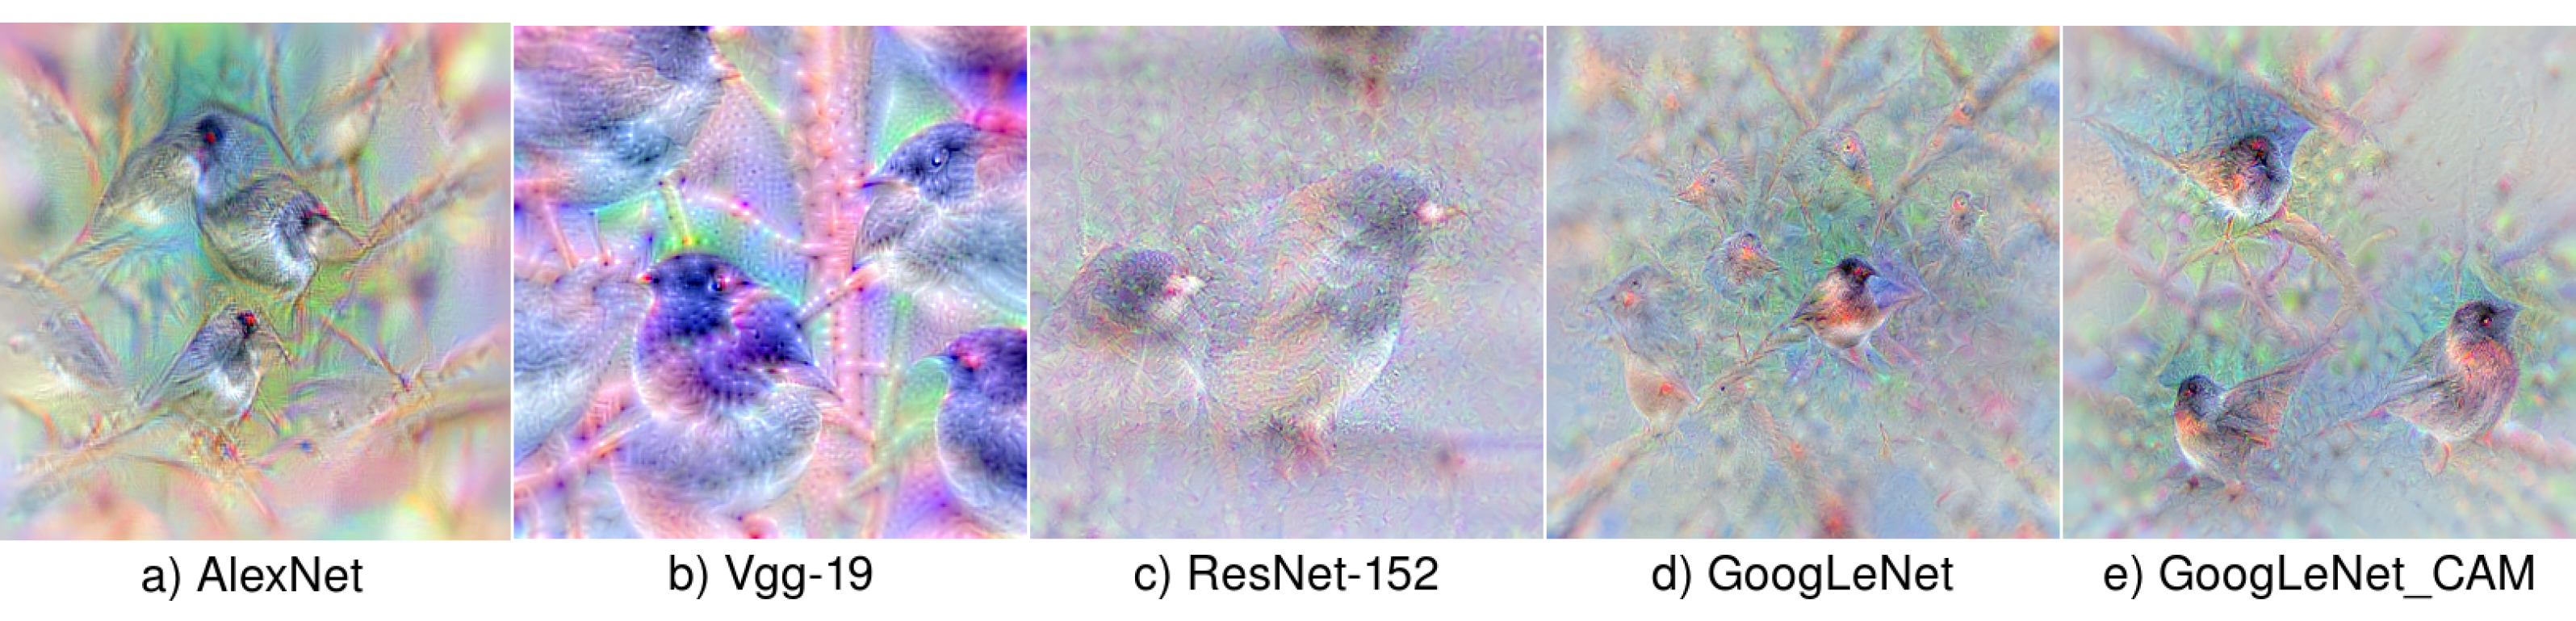
\includegraphics[trim = 0mm 35mm 00mm 35mm, clip, width=0.85\textwidth]{ch04_02}
%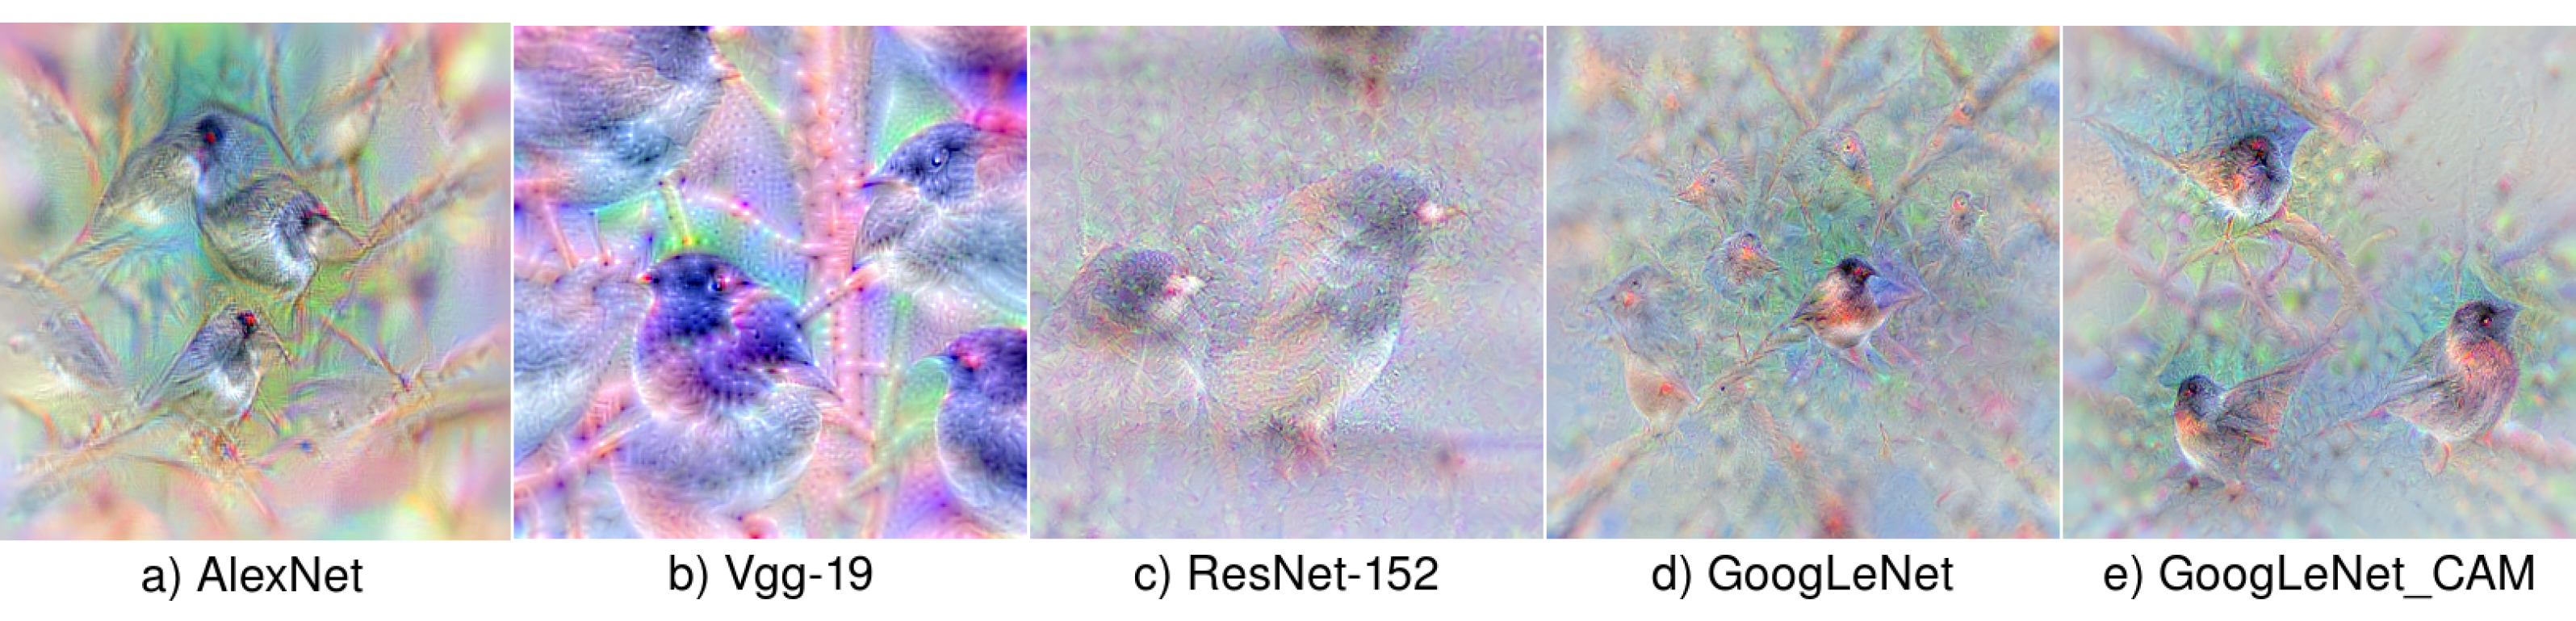
\includegraphics[width=0.85\textwidth]{ch04_02}
\caption{不同模型类别可视化实验结果}
\label{fig:ch04_02}
\end{figure}

实验选取的深度模型来自于开源社区的Caffe model zoo,不同的CNN模型如:AlexNet模型\citep{Krizhevsky2012},Vgg-19模型\citep{Simonyan2014a},Google-CAM模型\citep{Zhou2015},GoogleNet模型\citep{Szegedy2015},ResNet模型\citep{he15},其分类识别性能依次从低到高,模型的复杂程度依次递增。本文实验默认采用提出的梯度归一化,并引入多分辨率、随机扰动和剪切等小技巧作为通用设置,提高可视化效果。


为比较不同深度CNN模型学习相同类别时特征图的差异,根据式\ref{eq:ch04_01},给定高斯噪声生成随机图像作为输入,指定可视化物体类别向量(见图\ref{fig:ch04_02}所示,类别为所有类别中的第13类布谷鸟),施加前文提出不同正则化项的组合:p范数、高斯模糊和金字塔分解正则化。


图\ref{fig:ch04_02}结果表示5种CNN模型在相同正则化方法和相同梯度更新策略下的可视化效果,对比图\ref{fig:ch04_02}中a,b,c发现随着网络模型深度的增加,可视化难度增大分类性能同可视化效果一致;Vgg-19模型由于跟ResNet模型卷积核大小类似,且比AlexNet首层卷积核小(7和3),即可视化效果倾向生成比AlexNet更大尺寸的物体。而由图\ref{fig:ch04_02}中a,d,e对比可知,由于GoogleNet模型中卷积层的卷积核大小不一,使得可视化结果中引入更多细节。综合可知,基于GoogleNet模型的可视化效果最好,后面实验均是在其模型的基础上进行实验比较。

\subsubsection{ 不同正则化方法的类别可视化}
为验证不同正则化方法对理解深度模型的特征表达的影响,采取前文所述的不同正则化方法,可视化效果结果见图\ref{fig:ch04_03}所示,从上到下依次可视化类别为金甲虫,海星,蝎子,酒壶,卷笔刀。
 
\begin{figure}[!htbp]
\centering
%trim option's parameter order: left bottom right top
%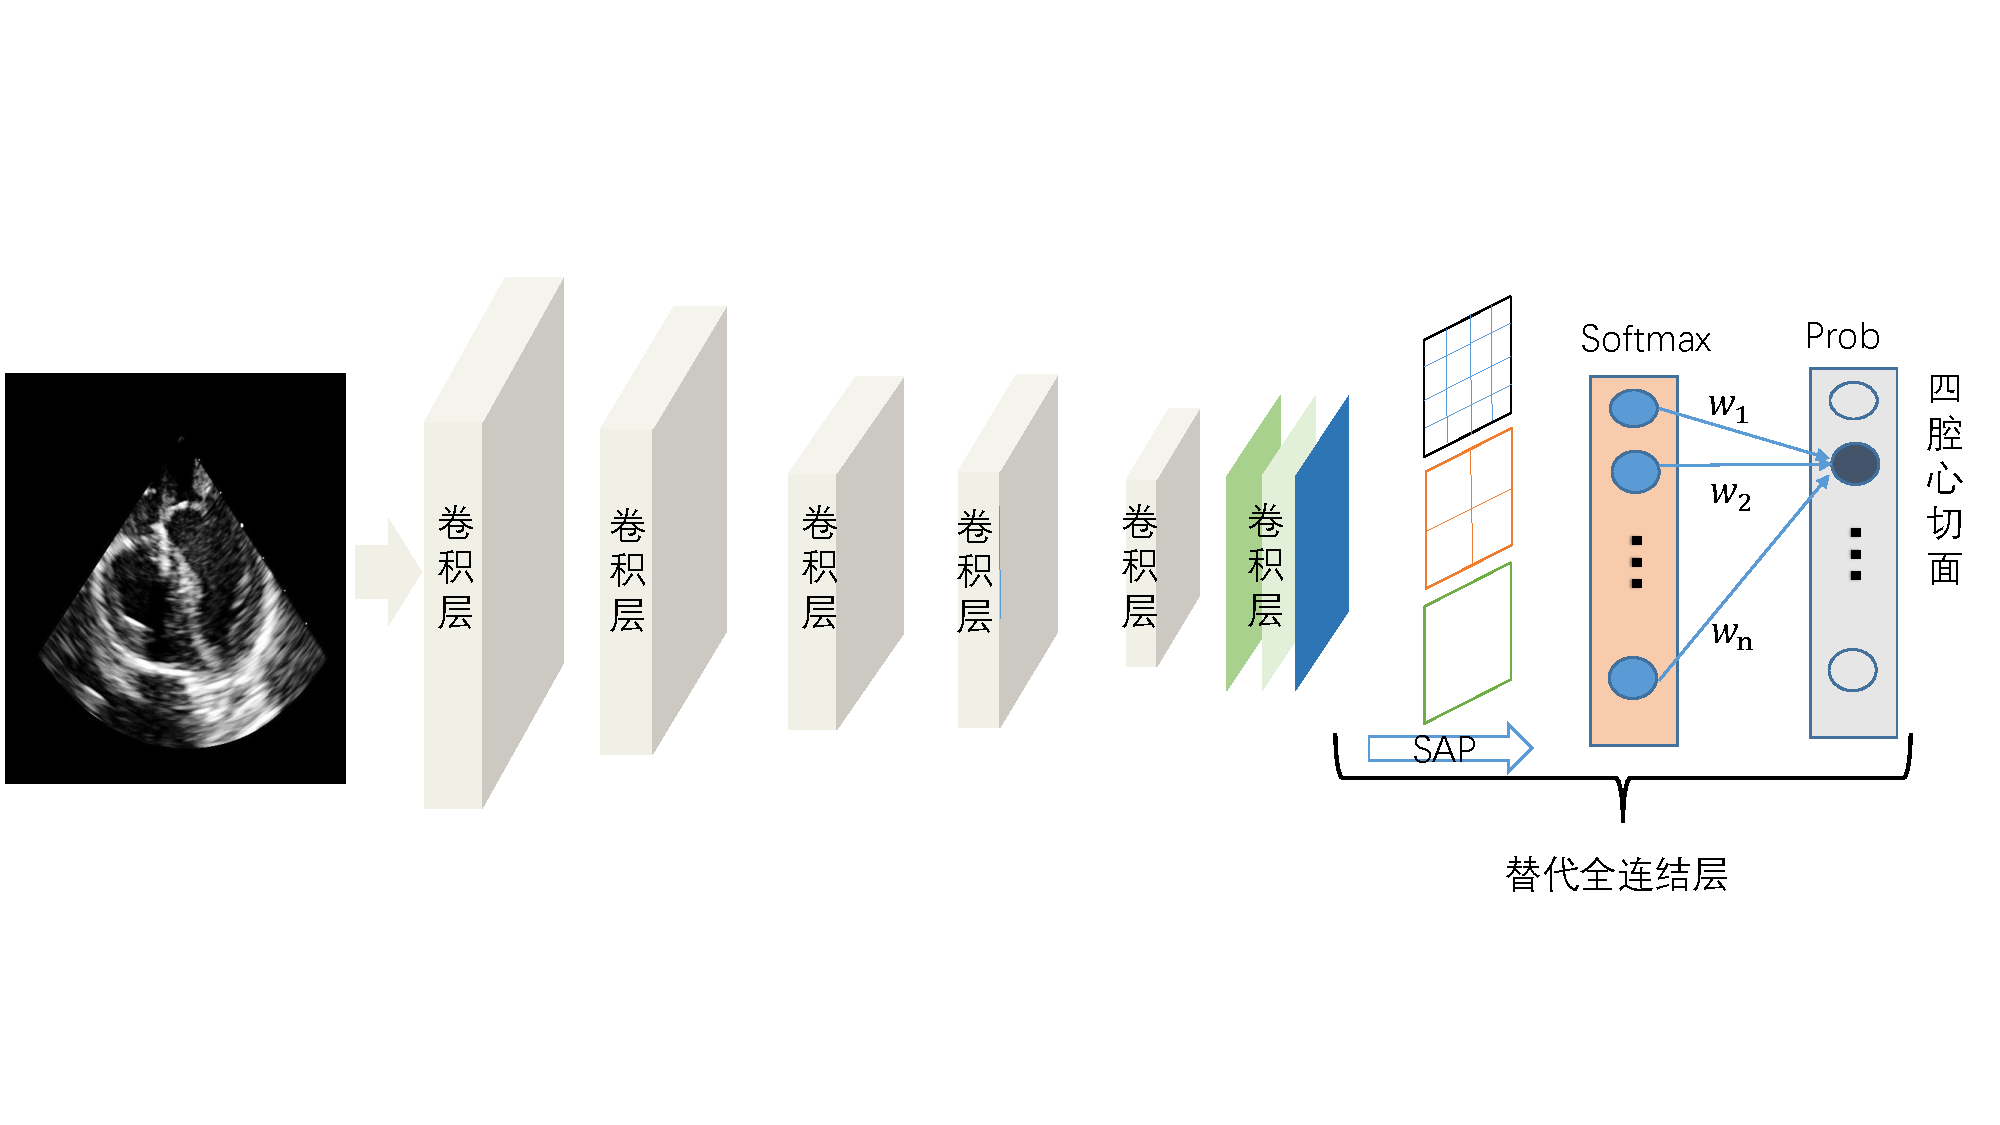
\includegraphics[trim = 30mm 0mm 30mm 0mm, clip, width=0.45\textwidth]{ch03_02}
\includegraphics[width=0.85\textwidth,height=0.4\textheight]{ch04_03}
\caption{不同正则化方法的可视化效果}
\label{fig:ch04_03}
\end{figure}

图\ref{fig:ch04_03}(a)列仅施加默认设置和不加梯度归一化的结果,由于输入的随机性,并不能保证每次都生成有意义的可视化结果,但引入本文提出的梯度归一化后,能大概率生成可视化结果见图\ref{fig:ch04_03}(b)列所示,图\ref{fig:ch04_03}(c)列表示只采用p范数正则化,跟文献\citepns{simonyan14deep}一致取2,使得图像更平滑,但仍与真实图像相差较大。通过前文理论分析和实验验证,全变分跟高斯模糊作用类似,本文采用根据迭代轮数动态调整高斯模糊核大小,具体是在刚开始采用较大值希望生成物体大概轮廓,随迭代逐渐调小模糊核使得更多细节生成,具体见图\ref{fig:ch04_03}(d)。但是这个参数无法自适应设置为最优,对图像高低频分量无法调整控制,而本文提出的利用金字塔分解正则化方法能从粗到细调整,产生较优结果见图\ref{fig:ch04_03}(e)列所示。

\subsection{金字塔分解可视化实验结果}

为验证提出金字塔分解正则化方法,对中间层卷积核的可视化,采用前文提出式\ref{eq:ch04_08},指定深度CNN模型中不同卷积层中不同通道,利用前文提出的带动量的梯度更新策略,可视化结果见图\ref{fig:ch04_04},其中从上到下依次为GoogleNet模型低中高层不同通道的可视化结果,与文献\citep{Zeiler2014}一致,低层多尺度分辨率生成的纹理见图\ref{fig:ch04_04}首行所示,中层是一些物体部件,见图4中间行所示蜜蜂的局部结构,而高层是更完整的抽象概念见图\ref{fig:ch04_04}下层中完整的花瓣。对比图\ref{fig:ch04_04}(b)、(c)列,可验证拉普拉斯金字塔主动分解提升图像部分低频成分,而高斯金字塔分解生成的图像中高频细节更突出。
\begin{figure}[!htbp]
\centering
%trim option's parameter order: left bottom right top
%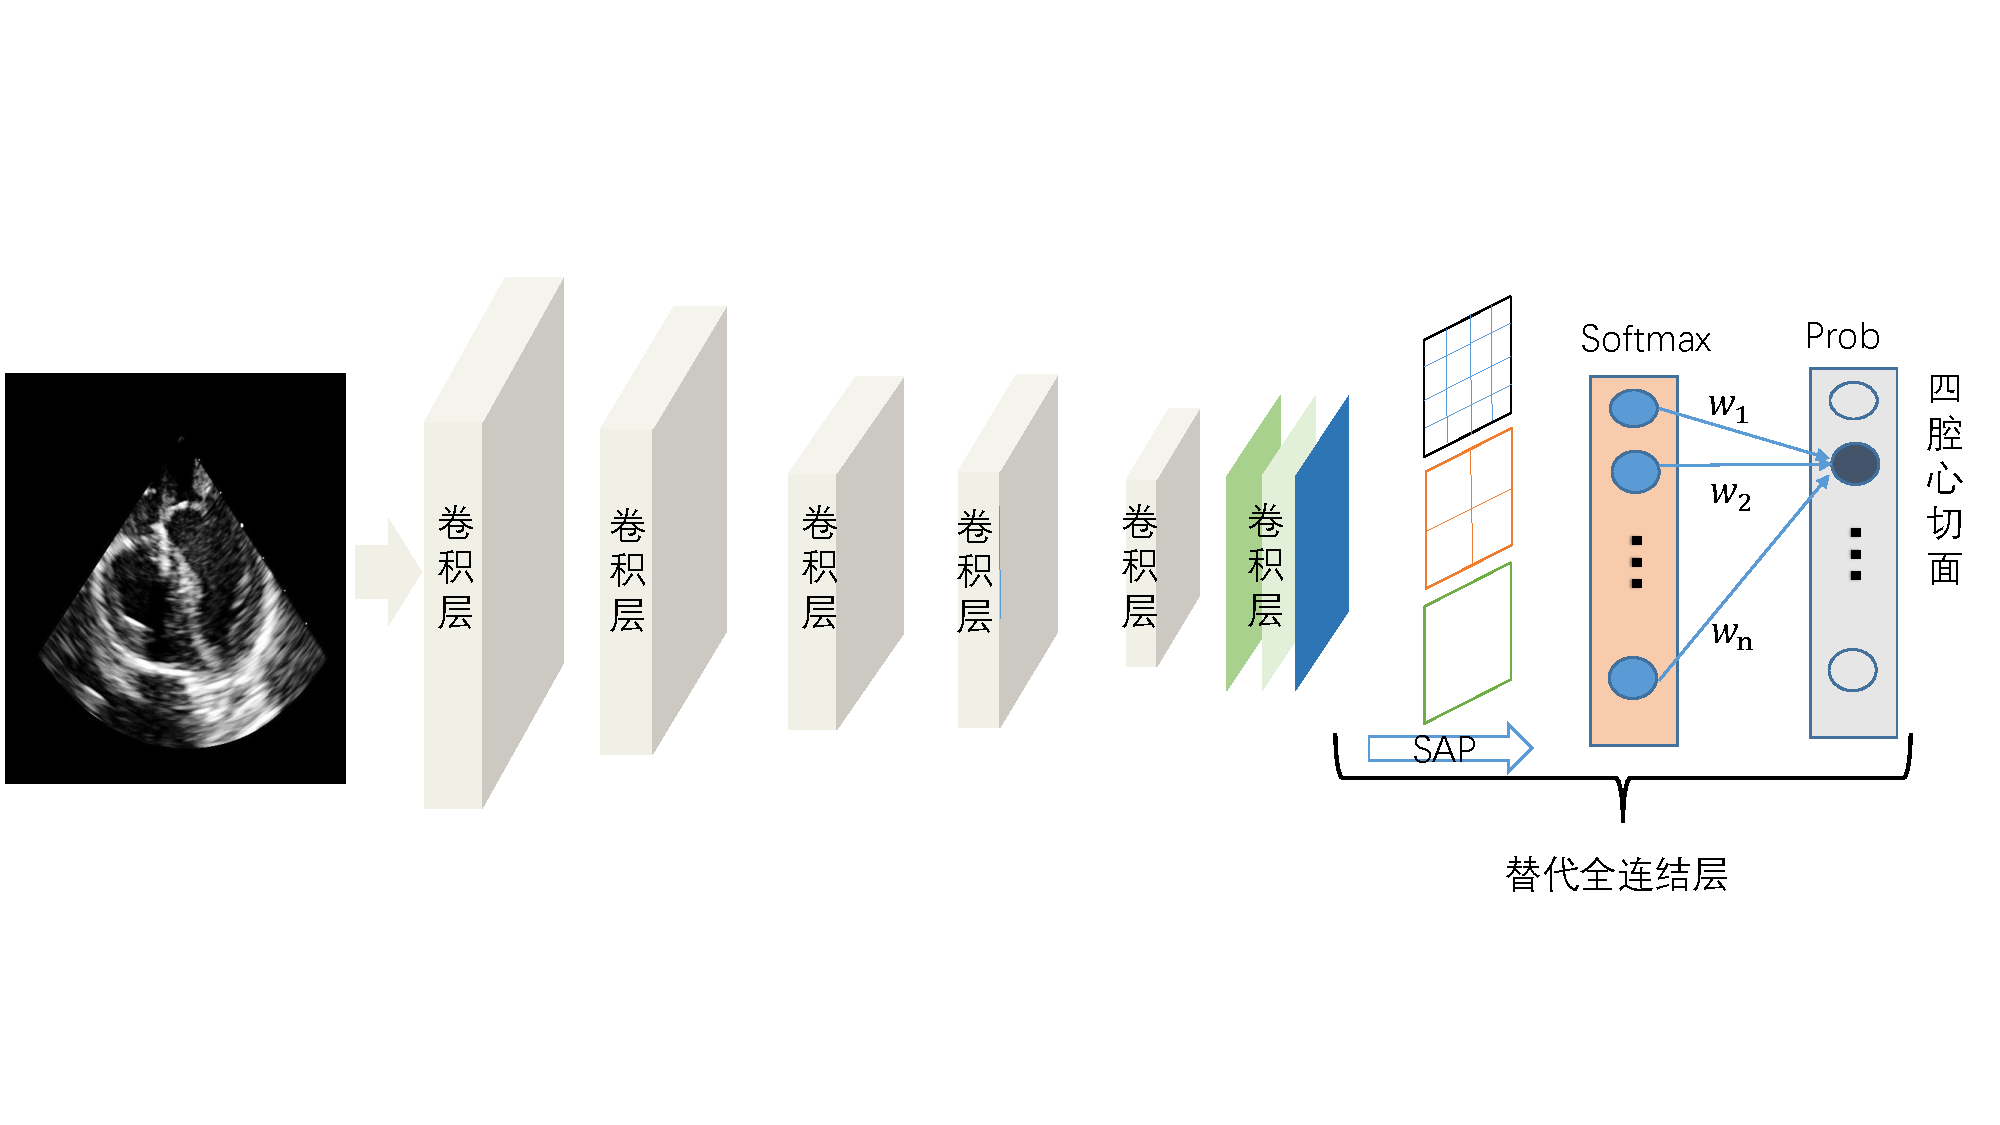
\includegraphics[trim = 30mm 0mm 30mm 0mm, clip, width=0.45\textwidth]{ch03_02}
\includegraphics[width=0.85\textwidth,,height=0.4\textheight]{ch04_04}
\caption{金字塔分解正则化可视化效果}
\label{fig:ch04_04}
\end{figure} 

\subsection{引入类别显著性的可视化} 

通过观察之前可视化结果可知,生成的图像中除了该类别外仍有许多额外的上下文信息(见图\ref{fig:ch04_02}中鸟类别的树枝),这些信息与模型的分类能力相关联,可通过引入类别激活图可改善可视化效果。迭代更新过程中依据采用式\ref{eq:ch04_11},使用类别激活图作为加权因子限制迭代更新区域。
\begin{figure}[!htbp]
\centering
%trim option's parameter order: left bottom right top
%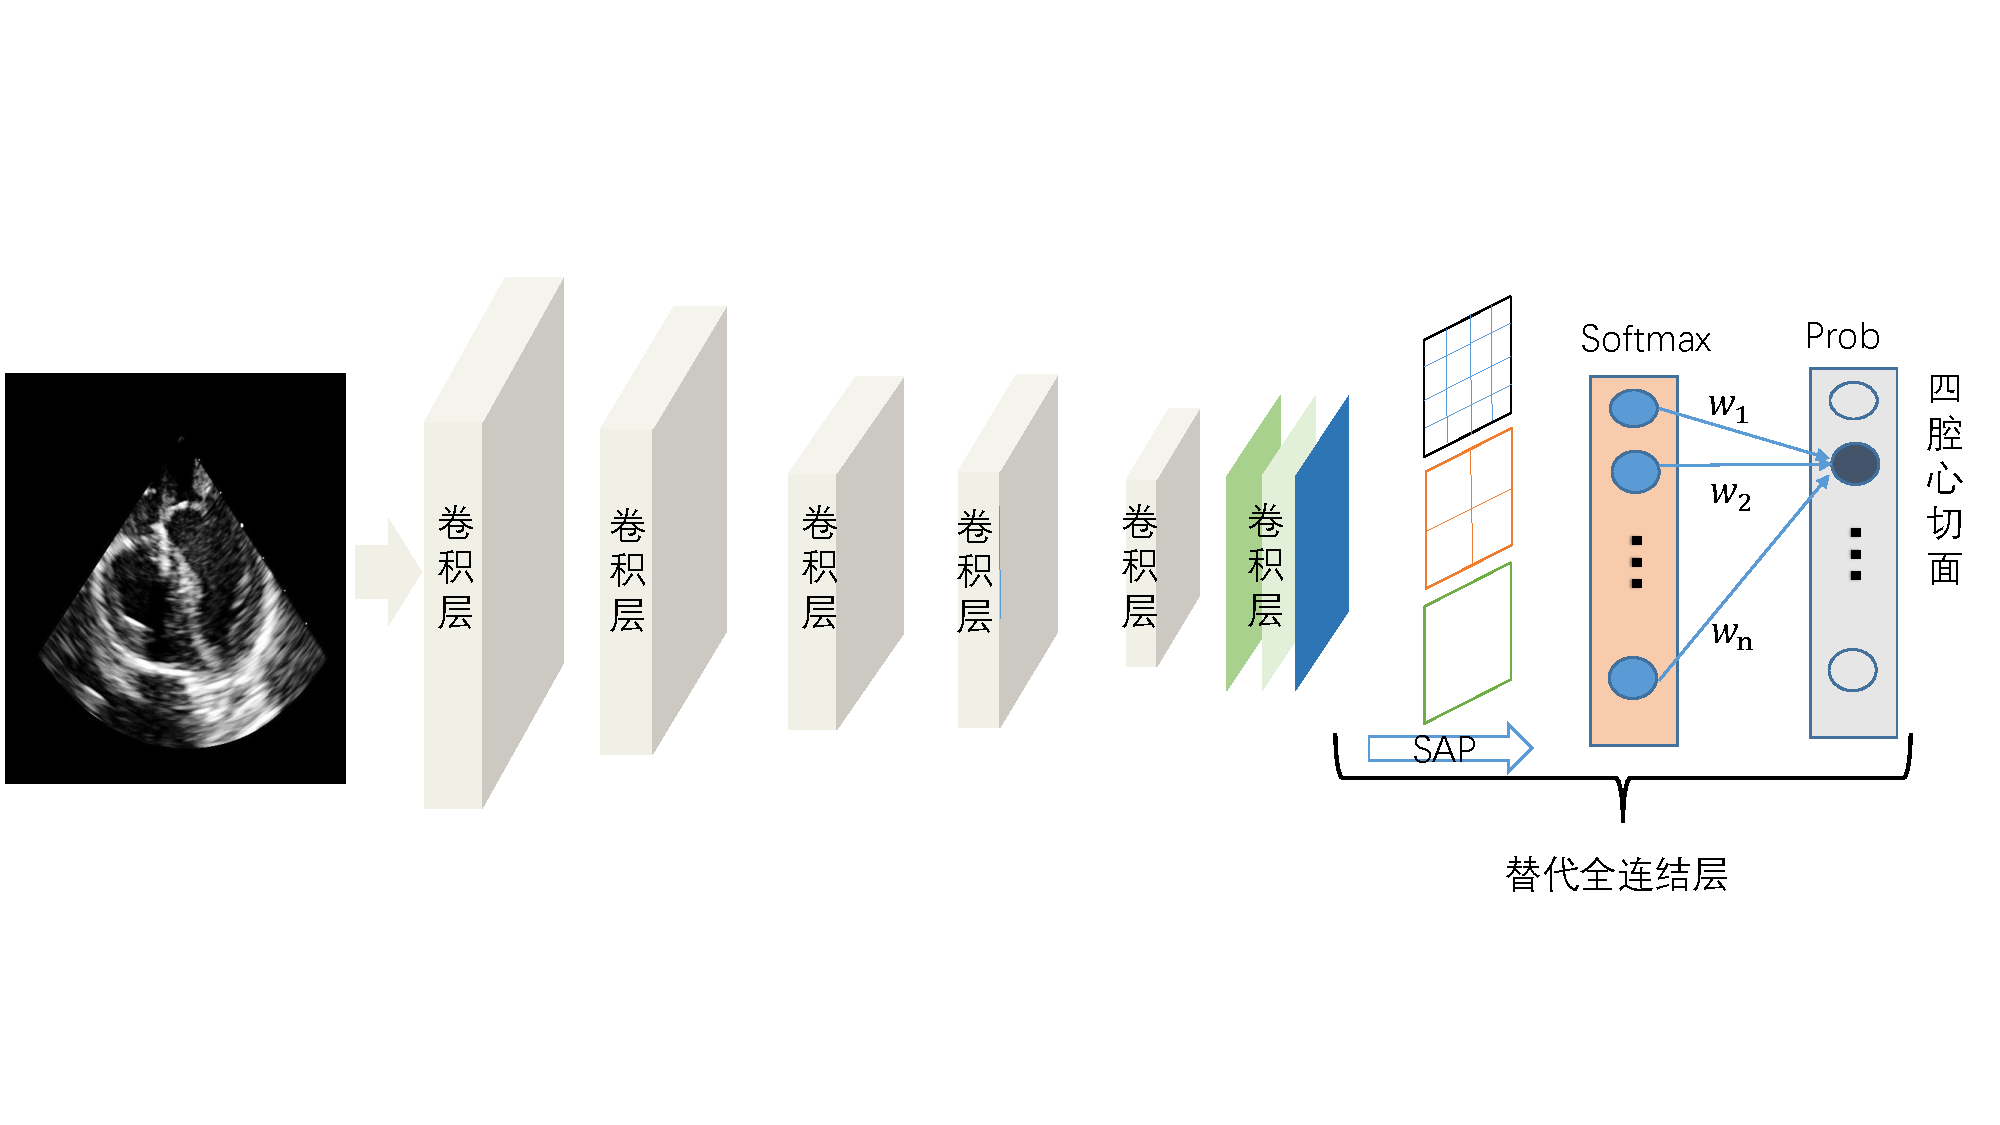
\includegraphics[trim = 30mm 0mm 30mm 0mm, clip, width=0.45\textwidth]{ch03_02}
\includegraphics[width=0.85\textwidth,,height=0.2\textheight]{ch04_05}
\caption{引入类别激活图的可视化}
\label{fig:ch04_05}
\end{figure}  

实验结果见图\ref{fig:ch04_05}(a)所示,具体实验设置和图2采用的参数一致,使用提出的金字塔分解正则化技术,图\ref{fig:ch04_05}(b)为图\ref{fig:ch04_05}(a)相应的类别激活图,图\ref{fig:ch04_05}(a)结果表明与类别无关的上下文信息得到压制,但仍存在两个类别中心。

\section{小结与讨论}

本文针对理解深度CNN特征空间存在的问题,提出一种用于改善深度CNN分类模型的可视化方法。其中通过改善激活最大化可视化技术来产生更具有全局结构的细节、上下文信息和更自然的颜色分布的高质量图像。该方法首先对反向传播的梯度进行归一化操作,在常用正则化技术的基础上,提出使用空间金字塔分解图像不同频谱信息;为限制可视化区域,提出利用类别显著激活图技术,可以减少优化产生重复对象碎片的倾向,而倾向于产生单个中心对象以改进可视化效果。激活最大化可显示CNN在分类时关注什么。这种改进的深度可视化技术将增加我们对深层神经网络的理解,进一步提高创造更强大的深度学习算法的能力。该方法适用于基于梯度更新的可视化领域,是对网络模型整体的理解,具体各层特征怎么耦合成语义信息仍需进一步探索,深度CNN模型如何重建一个完整的类别概念,仍是一个开放性问题。

\chapter{特征表示的中层结构性语义应用}
\label{chap:Detection}

\section{心室的计算机辅助检测方法}
计算机辅助检测(Computer-Aided Detections, CADs)是医学影像诊断过程中的一项重要任务,是进行相关结构功能测量的前提条件。其中,二维图像的目标组织结构自动检测是CADs技术的核心基础。在临床实践中,医生需整合不同模态、不同位置方向且以不同比例显示的图像信息,目前的研究主要关注如何使检测过程快速自动化。由于医学影像自身的特殊性,比如缺乏大量高质量标注数据;大多数医学目标组织结构存在非刚性形变;图像背景前景的区分不明显等,导致组织结构自动定位比较困难。现有大多数CADs系统在临床实际应用中表现不佳的原因是:检测结果的敏感性和特异性都较低,诊断效能低\cite{Cheng2016a}。


不同模态的医学图像中,如超声、计算机断层扫描和核磁共振等,都存在目标身体器官自动定位的问题。以左心室(Left Ventricle, LV)检测为例,大多数LV定位方法主要依据位置,时间和形状的假设。基于位置的方法仅假设心室在图像的中心,该方法并不对不同病人心室位置的差异性以及图像的尺寸变化进行考虑,效果较差;基于时间的方法,假设左心室是图像中唯一的运动对象,然而这种方法敏感性高,除心室的运动伪影之外,还存在其它运动的器官,如Schollhuber\citep{Schollhuber2008}针对MRI短轴使用时空信息并消除运动伪影,由分层模式匹配算法定位包含LV的感兴趣区域,其通过使用互信息图像配准使运动伪影最小化,随后估计特征强度—时间曲线进行像素分类和边界的提取,得到最终分割结果;基于形状的方法将LV视为圆(短轴)、椭圆(长轴),然而该方法通常针对异常形状的LV容错性差,如Lu等\citep{Lu2009}使用大津阈值度量圆形程度,然后进行霍夫变换定位LV位置。也可搜索每个切片的质心,并用三维最小二乘拟合去除异常值,得到分割结果\citep{Petitjean2011}。


不依据具体的强先验假设,机器学习算法可通过区分前景目标对象和背景来解决目标结构自动检测的问题。如Kellman等\citep{Lu2011}提出了一种使用概率集成提升树来估计LV姿态和用空间间隔学习LV短轴边界的方法。Zhou等\citep{Zhou2005}在超声心动图中通过规一化集成提升回归学习非线性映射以定位LV,其团队后来提出针对多个器官的特异性置信最大化分类器,整合更高的自由度以改善回归定位任务的精度。Liu等\citep{She2007}通过利用基于子模块函数优化理论的多标记搜索策略来进行标记点的检测。Zheng等\citep{Zheng2014}在实现器官定位的同时,通过组合优化置信度来估计目标器官的位置、缩放及朝向等参数值。前述机器学习算法都基于弱先验知识,启发式设计相关特征,结合滑动窗口策略,选择分类器进行分类判断窗口中内容以估计相应位置。


近来通用物体检测领域取得巨大进展,主要得益于深度学习能利用大量标注数据,从原始像素出发,逐层分级学习中高层抽象语义特征\citep{Sharif2014}。区域卷积神经网络\citep{Girshick2014b}在大规模自然图像数据集(如ImageNet\citep{Deng2009ImageNet})上,识别性能远超传统方法\citep{Girshick2014b,Krizhevsky2012}。当前实践中由于深度学习需要大量的训练数据,所以仅在少数医学任务中取得有限的成功应用。深度学习方法用在定位检测问题时可分为两个阶段\citep{Girshick2015b}:候选框位置选取和窗口内容类别分类。如利用深度卷积网络进行显微镜图像中细胞检测\citep{Akram2016}、结合深度全卷积网络的MRI心室检测与分割\citep{Emad2015,Tran2016a}和超声图像解剖结构的检测\citep{Chen2016i}。

上述方法大都关注特定目标结构的检测分割,而本文专门针对目前CADs普遍存在的检测定位问题,基于改进的生成候选框的快速区域深度卷积神经网络(Faster RCNN)\citep{Ren2015a}方法,提出一种医学目标结构检测框架:1)在区域生成网络的基础上引入空间变换损失使得候选框生成网络能捕捉目标的空间变换参数;2)采用在线困难样例挖掘策略,加快训练收敛过程,提高检测小目标的准确度;3)并基于目标先验知识,针对左心室提出利用检测二尖瓣环、心内膜垫和心尖位置,高效估计左心室姿态参数。4)为验证该算法的鲁棒性和有效性,分别针对两个具体CADs应用进行实验分析。

\section{区域卷积神经网络概览}
 
\subsection{物体检测形式化定义}
若用$r$来表示图像中的矩形窗口区域,令$R$表示由对象检测系统提供的所有候选窗口的集合,将有效定位标记定义为$R$的子集,使得标记位置内内容“不重叠”,令$Y$来表示所有有效标记位置的集合。并合并常用的非最大值抑制(Non-maximum suppression, NMS)过程,给定图像$x$和窗口评分函数$f$,物体检测算法流程可定义为\ref{alg:ch05_01}。
\begin{algorithm}[!htbp]
      \small
      \caption{物体检测算法}\label{alg:ch05_01}
      \begin{algorithmic}

          \State \textbf{输入:}{($x,f$)}\Comment{x为图像,f为窗口得分函数}
          \State $D$:= 所有候选框 $r \in$ 使得$f(x, r) > 0$  \Comment{一般采用滑动窗口}          
          \State 按 $f$ 排序$D$使得 $D1\geq D2 \geq D3 \geq ...Dn$ 
          \State 令$y^\star:=\{ \}$
          \State \qquad for $i = 1$ to $n$ do\Comment{一般采用非极大值抑制}
          \State  \qquad\qquad  若 $D_{i}$ 和 $y^\star$中任意候选框不重叠
          \State   \qquad \qquad      $y^\star$ := $y^\star  \bigcup {D_{i}}$
          \State \qquad\textbf{End} for 
          \State \textbf{Return:}  $y^\star$,物体的目标位置.
      \end{algorithmic}
  \end{algorithm} 
 
形式化定义物体检测过程见公式\ref{eq:ch05_01},式中参数定义请参考算法\ref{alg:ch05_01}。
\begin{equation} 
\label{eq:ch05_01}
      y^{\star}=\mathop{\arg\min}_{y\in Y}\sum _{r\in Y} f(x,r)
\end{equation}                               	 
通常公式\ref{eq:ch05_01}可通过贪心搜索的方法来完成,算法将联合最小化在算法\ref{alg:ch05_01}中产生假阳例的数量和最大化检测窗口评分函数,即寻找具有最大得分但同时不重叠的滑动窗口位置集合。
\subsection{区域卷积神经网络的演进}
2014年Gisrshick等\citep{Girshick2014b}提出区域卷积神经网络(Region-based Convolutional Neural Network, RCNN),对每一候选框窗口都进行一次前向传播,这将导致冗余计算,时间复杂度高,为解决这一问题,He和Ren等提出SPP-net\citep{He2015spp}和Fast RCNN\citep{Girshick2015b}加以改进,不再把每一候选窗口均送入网络,而是仅对图像特征提取一次,把原图中候选区域投影到卷积特征图上,然后对投影后的区域特征图进行空间感兴趣区域池化(ROI Pooling)得到固定长度的特征向量。
其中Fast RCNN中的感兴趣区域池化是SPP-Net中多尺度空间金字塔池化的特例,仅用单一尺度的金字塔池化操作。RCNN及其改进的Fast RCNN都依赖于人为设计的候选框生成方法,如选择性搜索等。为减少生成候选框的计算时间,Faster RCNN提出区域生成网络(Region Proposal Networks,RPN),区域生成网络和检测网络共享提取特征的卷积层,仅提取几百个或者更少的高质量预选窗口,且召回率较高(导致更少的假阳例)。但现有的通用物体检测算法均是假设候选框为矩形,不能解决旋转朝向问题。

\section{候选区域生成网络及其改进}
 
本章将分别从候选区域生成网络模型的结构、仿射变换候选框区域的生成、空间变换损失函数的设计、模型训练方法等方面介绍本文所提出框架,并结合Faster RCNN模型提出端到端的目标检测方法。

\subsection{候选区域生成网络模型结构}

候选区域生成网络将一图像(任意大小)作为输入,输出目标候选框的集合和每个候选框内有无目标的概率估计,如图\ref{fig:ch05_01}右图所示,RPN在卷积层后接两个全卷积层完成候选区域生成功能,以实现增加滑动窗口操作。该模型使用全卷积网络[20]处理任意大小的图片输入,为了和目标检测网络\citep{Girshick2015b}共享计算,在特征提取的过程中同时计算目标检测所需的感兴趣区域的初始估计,在最后一个共享卷积层输出的特征映射图上滑动小网络,卷积特征映射图上n×n大小空间窗口作为该网络全连接的输入,本文n取3。
每个滑动窗口映射到一个低维向量上(如图\ref{fig:ch05_01}左上中256-d),该向量输出给两个全连接层——候选框位置定位回归层和候选框类别分类层。原文中采用类别无关分类损失,即仅区分该候选框内是否包含物体(前/背景),本文将其扩展为类别相关的分类损失。

\begin{figure}[!htbp]
\centering
%trim option's parameter order: left bottom right top
%\includegraphics[trim = 30mm 0mm 30mm 0mm, clip, width=0.45\textwidth]{ch03_02}
\includegraphics[width=0.9\textwidth]{ch05_01}
\caption[区域生成网络模型的各个组件图]{左上:引入空间不变性的anchor机制 左下:空间变换网络  右:Faster R-CNN带仿射变换的检测模型框架}
\label{fig:ch05_01}
\end{figure}

为引入空间尺度不变性,采用多尺度和多纵横比的“参考”框(anchor),如图\ref{fig:ch05_01}左上所示。该机制可看作是金字塔型参考框的回归,避免了枚举多尺度、多纵横比的图像或卷积核。
在每一个滑动窗口的位置,同时预测$k$个参考区域,回归层有$4k$个输出,即$k$个box的坐标编码
,多元逻辑回归分类层输出$(c+1)×k$个(物体类别数$c$加背景类的)概率估计。
候选框由相应的$k$个anchor的参数化表示,每个anchor以当前滑动窗口中心为中心,
并对应一种尺度和长宽比,我们使用3种尺度和3种长宽比,在每一个滑动位置就有$k=9$个anchor。
对于大小为w×h的卷积特征映射,总共有$w \times h\times k$个anchor。

\begin{figure}[!htbp]
\centering
%trim option's parameter order: left bottom right top
%\includegraphics[trim = 30mm 0mm 30mm 0mm, clip, width=0.45\textwidth]{ch03_02}
\includegraphics[trim = 30mm 0mm  30mm 0mm,width=0.95\textwidth]{ch05_02}
\caption[考虑物体朝向的区域生成网络模型结构示意图]{考虑物体朝向的区域生成网络模型结构示意图,图中conv表示卷积层,pool表示池化层,FC表示全连接层,softmax class loss表示多任务损失中的分类损失,Bbox.reg loss 表示候选框回归定位损失,Rotation loss表示文中的针对变换参数θ的Von Mise损失。}
\label{fig:ch05_02}
\end{figure} 

\subsection{仿射变换候选框}
 
为检测物体的姿态,结合空间变换网络\citep{Jaderberg2015}(见图\ref{fig:ch05_01}左下),提出带仿射变换的候选框生成算法。之前的候选框生成方法仅考虑固定尺度和宽高比的矩形框,并未考虑物体的旋转朝向,二维空间仿射变换可表示为:
\begin{equation} \label{eq:ch05_02}
\begin{pmatrix}
x_{i}^{s}\\ 
y_{i}^{s}
\end{pmatrix} =\tau _{\theta}\begin{pmatrix}
x_{i}^{t}\\ 
y_{i}^{t}\\
1
\end{pmatrix}=\begin{bmatrix}
\theta_{11} &\theta_{12}  &\theta_{13} \\ 
 \theta_{11}&\theta_{22}  & \theta_{23}
\end{bmatrix}\begin{pmatrix}
x_{i}^{t}\\ 
y_{i}^{t}\\
1
\end{pmatrix}
\end{equation}                    
式中$(x_{i}^{s},y_{i}^{s})^T $为输入特征图中目标坐标系下的网格点,$\tau _{\theta}$ 为变换矩阵,$(x_{i}^{t},y_{i}^{t})^T $为输出特征图中目标坐标系下的采样网格点。其中由于图像的坐标不是中心坐标系,宽高坐标需归一化表示,如$-1\leq x_{i}^{s},y_{i}^{s}\geq 1$,且采用图形学中齐次坐标表示。公式\ref{eq:ch05_02}能用六个参数定义对输入特征图的裁剪、平移、旋转和缩放等变换。该公式进步简化为只考虑旋转变换:
\begin{equation} \label{eq:ch05_03}
\begin{pmatrix}
x_{i}^{s}\\ 
y_{i}^{s}
\end{pmatrix} =\tau _{\theta}\begin{pmatrix}
x_{i}^{t}\\ 
y_{i}^{t}\\
1
\end{pmatrix}=\begin{bmatrix}
\cos\alpha &-\sin\alpha  &0 \\ 
 \sin\alpha&\cos\alpha  & 0
\end{bmatrix}\begin{pmatrix}
x_{i}^{t}\\ 
y_{i}^{t}\\
1
\end{pmatrix}
\end{equation}  
其中 $\alpha$表示绕图像中心顺时针旋转角度,通常变换后的像素并不是在相应网格的整数值,常用双线性插值进行近似,变换后的候选框送入感兴趣区域池化层,后接多任务损失函数。实质是把空间变换层嵌入到RPN网络中,并且引入有监督的损失以指导空间变换。
\subsection{朝向回归损失函数}

旋转朝向的周期性会导致两个问题:(1)要优化的损失函数不能区分对于周期性损失,简单地将模运算符应用于网络的输出会导致不可靠的损失,不能再被鲁棒地优化。(2)由大多数参数模型中执行的矩阵向量积产生的回归输出是固定的线性运算。为此提出旋转朝向回归损失$L_{VM}(o,o^{*})$,第一个问题可以通过采用Von Mise 分布\citep{Beyer2015}来解决损失函数不连续性,其近似服从于单位圆上的正态分布:
\begin{equation} \label{eq:ch05_04}
      p_{VM}(\varphi \mid \mu,k)=\frac{e^{k \cos(\varphi-\mu)}}{2\pi I_{0}(k)}
\end{equation} 	                            	  					             
其中$p$指相应的概率密度函数,$\varphi$ 指角度,$\mu $ 是分布的平均角度,$k$ 与近似高斯方差成反比,而$I_{0}(k)$  是阶数为0的修正贝塞尔函数,利用余弦函数来避免不连续性,可以得出以下损失函数:
 \begin{equation} \label{eq:ch05_05}
      C_{VM}(\theta \mid t,k)= 1- e^{k (\cos(\theta-t)-1)}
\end{equation}         			                    
式中$\theta$ 为预测旋转角度大小,$t$为真实旋转角度大小,称$t$为目标值,$k$为控制损失函数尾部的简单超参数。由角度$varphi$ 正余弦组成的二维向量$y=(\cos\varphi,\sin\varphi)$ 替代表示,利用自然语言处理文献中广泛使用的余弦代价函数[31]来解决使用线性操作来预测周期值的问题:
\begin{equation} \label{eq:ch05_06}
     C_{\cos}(y \mid t)=1- \frac{y\times t}{\parallel y\parallel \parallel t\parallel}  
\end{equation}      					               
在神经网络框架中的实现是相对简单的,因为所需要的是全连接层和归一化层,前向传播公式:
\begin{equation} \label{eq:ch05_07}
      f_{BT}(x \mid W,b)=\frac{Wx+b}{\parallel Wx+b \parallel }
\end{equation}  
                     			                    	 
式中 $W\in R^{n\times 2}$ 和 $b\in R^{2}$ 是来自全连接层的可学习参数,然后反向传播归一化损失的导数为
\begin{equation} \label{eq:ch05_08}
      \partial _{x_{i}} \frac{x}{\parallel x\parallel}=\partial _{x_{i}}\frac{x }{\sqrt{\sum_{j}x_j^2}} =\frac{\sum_{j \neq 
 i}x_j^2 }{(\sum_{j}x_j^2)^{\frac{3}{2}}}  =\frac{\sum_{j \neq i}x_j^2 }{\parallel x\parallel^3} 
\end{equation} 	                 			    
式中归一化确保输出值被联合学习,通过比较$CVM$和$Ccos$,最终朝向回归损失函数为
\begin{equation} \label{eq:ch05_09}
      L_{VM}(y\mid t) = 1- e^{k (y\times t-1)}
\end{equation} 	                           								
与式\ref{eq:ch05_06}相似,主要区别在于存在e,它将目标值附近的错误“下推”,实际上是较小地惩罚小错误。

\subsection{带朝向的多任务损失函数}

多任务损失分别存在于RPN及检测网络中,图2中显示的是检测网络结构示意图。每一个候选框均送感兴趣池化层,后接两层的全连接层和多元逻辑回归分类损失(图\ref{fig:ch05_02}中Softmax loss),候选区域回归定位损失(图\ref{fig:ch05_02}中Box.reg loss)和旋转朝向回归损失(图\ref{fig:ch05_02}中Rotation loss):
\begin{equation} \label{eq:ch05_10}
      L(p,p^*,t,t^*,o,o^*)=L_{cls}(p,p^*)+\lambda[p^*> 0]L_{box}(t,t^*)+\mu [p^*> 0]L_{VM}(o,o^*)
\end{equation} 

式中,分别代表预测类别分类概率,候选框偏移量和感兴趣区域内物体的朝向大小; 表示标记类别为背景,表示框内是否有目标的指示函数,分别表示物体的候选框标记和真实朝向。为两个损失的相应平衡权重大小,详细形式如下:
\begin{equation} 
\label{eq:ch05_11}
      L_{(cls)}(p,p^*)=-\sum_{c}\log p_{c}^*
\end{equation} 

 \begin{equation} \label{eq:ch05_12}
      L_{box}(t,t^*)=-\sum_{i \in {(x,y,w.h)}}smooth_{L1}(t^*-t)
\end{equation} 

\begin{equation} \label{eq:ch05_13}
smooth_{L1}(x)= \left\{
     \begin{matrix}
0.5x^2 & if \mid x\mid<1 \\
 \mid x\mid-0.5 & else \\
\end{matrix}\right.
\end{equation} 

 $L_{cls}(p,p^*)$和$L_{box}(t,t^*)$ 是公式\ref{eq:ch05_04}中的分类损失和相应的平滑L1损失,$c$代表类别数。
\subsection{困难样例挖掘}

由于医学数据样本标注困难,数量相对较少,一般假设与目标位置矩形框有重叠的候选框是有较大概率是难以区分的,结果也可能是次优的,因为在其他位置可能存在更难区分的样本,导致模型收敛变慢,误警率高。在每次迭代训练过程中采用在线困难样例挖掘方法(Online Hard Example Mining,OHEM)\citep{Shrivastava2016a},对所有候选框的损失进行排序,由于相似候选框重叠区域的损失很接近,可采用非极大值抑制策略限制候选框的数目,选择前$k$个最大损失作为困难样例,反向传播其相应的梯度,其他候选框的梯度不进行回传,即不更新模型权重。

\section{实验结果分析和讨论}
 
为验证提出的自动检测算法的有效性和正确性,本节将分别采用一个公开可用的MRI数据集,和我们收集的来源于四川大学华西医院麻醉科的经食道超声心动图数据集(不包含患者信息)上进行实验。相关实验代码请参考\footnote{https://github.com/taopanpan/echodetection}。

\subsection{检测MRI左心室短轴}

纽约大学提供的公用数据集\citep{Andreopoulos2008}包含33名患者的心脏MRI体数据,以及LV心内膜和心外膜的手动分割结果。该数据集中的大多数切片包含心脏疾的病例切片。该数据集使用 GE Genesis Signa MRI扫描仪,采取FIESTA方案扫描获得。每个患者的20个序列帧包含8-15个短轴切片,大小为256x256,厚度为6-13 mm,像素分辨率为0.93-1.64 mm。为了检验所提出方法定位性能,取14个体数据形成1176个切片作为训练集,其余作为测试集。本实验中不使用旋转朝向损失,评价指标采用文献\citepns{Emad2015}中定量评估计算左心室短轴(SAX)定位的准确度,敏感性和特异性。

\begin{table}[!htbp]
    \centering
    \caption{不同模型检测精度的比较表}
    \footnotesize% fontsize
    \setlength{\tabcolsep}{4pt}% column separation
    \renewcommand{\arraystretch}{1.2}%row space 
    \begin{tabular}{lccc}
        \cline{1-4}% partial hline from column i to column j
            Method  & Accuracy & Sensitivity &Specificity \\
        \hline
        Baseline\citepns{Ren2015a} & $95.06\%$ & $73.91\%$ & $97.56\%$\\
        \hline
        VGG16 & $96.35\%$ & $74.68\%$& $99.26\%$ \\
        \hline
        ResNet101 & $98.66\%$ & $76.81\%$& $99.16\%$ \\
        \hline
        VGG16\_OHEM & $96.56\%$ & $79.42\%$& $99.07\%$ \\
        \hline
        ResNet101\_OHEM & $\textbf{99.49\%}$ & $\textbf{83.12\%}$ & $\textbf{99.40\%}$\\
        \hline\hline
    \end{tabular}
    
    \label{tab:ch05_02}
\end{table}

为评价不同深度模型对检测效果的影响,实验的检测模型选取VGG16\citep{Simonyan2014a}和ResNet101\citep{he15},训练方法采取端到端的近似联合优化,OHEM表明训练过程中采用困难样例挖掘方法,即在训练中只选择损失占前70\%的样本进行反向传播。训练参数及实现跟文献\citepns{Ren2015a}中一致,迭代次数为1000,以文献\citepns{Ren2015a}方法作为基准(表\ref{tab:ch05_02}中Baseline),评价指标采用通用的定位精度、敏感性和特异性,结果见表\ref{tab:ch05_02}所示,在测试集上最优检测准确度99.49\%,敏感性83.12\%,特异性为99.40\%,与基准检测模型相比精度提高了超过3\%,同时提高了约1.5\%的特异性。

另一方面,敏感性是最容易提高的参数,平均超过8\%,模型不能正确定位为大尺寸的心脏,导致较小LV切片的高FP,降低了整体系统性能。而困难样例挖掘的方法没有显著提高特异性,因为TN和FP都降低。考虑到心脏异常的高变异性导致心脏形状的大变异性,所提出的算法均能成功定位LV短轴,当检测出心室短轴时,可大致确定心室中心点(如图\ref{fig:ch05_04}(a)所示),利用二腔心(2CH)和四腔心切面(4CH)均垂直于短轴切面的先验,找到与SAX的2CH和4CH交集在SAX平面上投影,然后得到投影线在2D图像上相交的位置,即为左心室的3D位置(如图\ref{fig:ch05_04}(b)所示)。

\subsection{检测左心室及其朝向}

MRI左心室短轴的检测由于组织结构相对简单,且噪声少。为验证提出算法的通用性,针对超声图像左心室长轴切面检测心室、二尖瓣环、心内膜垫和心尖位置,并估计左心室朝向。主要包含单扇形和多普勒成像的双扇形两种由专业医师标注食管中段四腔心(ME4C) 的标准切面视频构成,视频中至少包含2-3个心动周期,依据医师建议从视频中截取5帧,并经医师检验手工筛选后得到900张ME4C切面,对切面内左心室(LV),二尖瓣环、心内膜垫和心尖位置进行人工标注作为“金标准”。其中随机选取100张作为测试集,其余作为训练集。
训练时采用提出的联合多任务损失,以VGG16网络作为检测的预训练的模型为例,在RPN中添加空间变换网络实现了各个候选框的空间变换,并施加旋转朝向损失。VGG16网络特征提取器包括13个卷积层,并输出512个conv5特征图,空间变换网络包括具有两个同样卷积池化层组成的定位网络,其由20个卷积核大小为5、步长为1和核大小为2的池化层构成,两层全连接层回归得出6个仿射变换参数,其中,全连接层的激活函数需选择为双曲正切函数,权重高斯初始化,而变换参数初始化为$[1, 0, 0, 0, 1, 0]^T$。其它跟Faster RCNN中设置一致,其中$\lambda$、$\mu$,分别取0.1和0.001;训练方法采取端到端的近似联合优化,迭代轮数为50000。评价指标采用平均检测精度(mean average precision,mAP),是多个类别平均检测精度的平均值。表二显示使用提出方法分别在VGG16模型和ResNet101模型上,结合困难样例挖掘训练方法得出的测试结果,其中OHEM表示相应模型结合在线困难样例挖掘方法的检测结果,STN表示结合提出带朝向损失的空间变换网络的检测结果,在测试集上,针对左心室的AP最优可达99.12\%,结果表明提出算法在不同基础模型上均可提高检测精度。

\begin{table}[!htbp]
    \centering
    \footnotesize% fontsize
    \setlength{\tabcolsep}{4pt}% column separation
    \renewcommand{\arraystretch}{1.2}%row space 
    \begin{tabular}{lccccc}
        \cline{1-6}% partial hline from column i to column j
           \qquad Method  & MAP & lv &apx &left &right\\
         
        \hline
        VGG16\_OHEM & $80.11\%$ & $90.12\%$& $65.46\%$ & $81.27\%$& $83.53\%$\\        
        \hline
        VGG16\_OHEM\_STN & $82.05\%$ & $90.92\%$& $66.57\%$& $86.16\%$& $84.46\%$ \\
        \hline
        ResNet101\_OHEM & $83.06\%$ & $95.72\%$& $66.39\%$& $85.25\%$& $84.83\%$ \\
        \hline
        ResNet101\_OHEM\_STN & $\textbf{85.59\%}$ & $\textbf{99.12\%}$ & $\textbf{67.89\%}$ & $\textbf{87.66\%}$ & $\textbf{87.48\%}$\\
        \hline\hline
    \end{tabular}
    \caption[不同模型的检测精度表]{不同模型的检测精度表,其中LV表示左心室,Apx代表心尖,left代表二尖瓣环,right代表心内膜垫}
    \label{tab:ch05_03}
\end{table}


为验证提出算法在检测左心室位置的同时可以回归学习左心室的姿态参数、预测左心室的朝向变换,超参数k跟文献\citepns{Beyer2015}一致,交叠比大于0.5时估计姿态参数,人为标定心室朝向存在较大偏差,但可以根据二尖瓣环、心内膜垫和心尖位置估算出心室朝向角度作为对照。由于ME4C切面中心室的大概朝向的分布范围在$[-45^{\circ},45^{\circ}]$之间,通过手工构建训练集,训练样本旋转以$15^{\circ}$为间隔的指定角度。通过分析相关估算结果和预测结果,可以发现二者具有很大的一致性。左心室检测结果和旋转朝向结果见表\ref{tab:ch05_03},检测结果如图\ref{fig:ch05_04}(c,d)所示,更多实验结果请参考给定开源地址。
\begin{table}[!htbp]
    \centering
    \footnotesize% fontsize
    \setlength{\tabcolsep}{4pt}% column separation
    \renewcommand{\arraystretch}{1.2}%row space 
    \begin{tabular}{lccccccc}
        \cline{1-8}% partial hline from column i to column j
            Method  & $-45^{\circ}$ & $-30^{\circ}$ & $-15^{\circ}$ & $+15^{\circ}$ & $+30^{\circ}$&$ +45^{\circ}$& Avg\\
         
        \hline
        Compute & $66.65\%$ & $78.02\%$& $87.39\%$& $85.53\%$& $75.83\%$ &$62.31\%$ &$75.94\%$  \\
        \hline
        Pred & $\textbf{73.09\%}$ & $\textbf{81.72\%}$ & $\textbf{81.75\%}$ & $\textbf{89.56\%}$ & $\textbf{80.48\%}$& $\textbf{70.31\%}$& $\textbf{80.76\%}$\\
        \hline\hline
    \end{tabular}
    \caption[不同旋转角度分类检测性能比较]{不同旋转角度分类检测性能比较,Compute表示根据额外标记计算得到的结果,Pred表示模型预测结果}
    \label{tab:ch05_04}
\end{table}

为了更详细地评估模型性能,使用检测分析工具\citep{Hoiem2012}分析了心尖位置的检测结果,如图\ref{fig:ch05_03}显示模型可以准确(白色区域)检测到心尖位置,召回率在84-87\%左右,并且比“弱”标准(小于0.1交叠比)高得多。针对心尖位置的定位精确度较低,这是因为医师在标定心尖位置时有很大的随意性,且目标尺寸较小,与类似对象类别有更多的混淆。
\begin{figure}[!htbp]
\centering
%trim option's parameter order: left bottom right top
%\includegraphics[trim = 30mm 0mm 30mm 0mm, clip, width=0.45\textwidth]{ch03_02}
\includegraphics[height= 30mm,width=0.9\textwidth]{ch05_03}
\caption[利用检测分析工具\citep{Hoiem2012}的检测结果]{利用检测分析工具\citep{Hoiem2012}的检测结果,左图显示apx检测精度的累积分布:正确的(Cor)或定位不准确(Loc)的假阳性,与之混淆类似类别(Sim)与其他类别(Oth)或背景(BG)。固体红色线是以“强”标准(大于0.5 交叠比),反映精确度随检测增加而变化。红色虚线使用“弱”标准(大于0.1交叠比)。右图显示排名靠前的假阳性类型的分布。}
\label{fig:ch05_03}
\end{figure} 	                          
 
\begin{figure}[!htbp]
\centering
%trim option's parameter order: left bottom right top
%\includegraphics[trim = 30mm 0mm 30mm 0mm, clip, width=0.45\textwidth]{ch03_02}
\includegraphics[height= 30mm,width=0.9\textwidth]{ch05_04}
\caption[医学图像目标检测结果示意图]{(a,b) 表示不同MRI图像检测左心室结果,(c,d)两图表示超声心动图的ME4C切面的左心室、二尖瓣环、心内膜垫和心尖位置及旋转角度的检测结果。}
\label{fig:ch05_04}
\end{figure} 	                         
 
\section{小结与讨论}

本文利用深度学习来解决医学图像计算机辅助检测问题,设计并验证了自动检测MRI短轴和超声心动图中LV长轴切面的方法,在通用物体检测Faster RCNN框架的基础上,针对RPN引入空间变换,结合带朝向损失的多任务损失,探索解决图像平面内物体旋转角度检测的问题,并利用困难样例挖掘策略加快迭代训练。在公共MRI数据集和自主收集的超声心动图数据上进行详尽实验验证,在多个评估指标方面提供更好的测试结果,但该方法仍耗费较多的标注数据,探索需要更少标注数据的检测算法是将来的工作目标。本章研究内容和主要成果以题为《基于深度学习的医学计算机辅助检测方法研究》的论文形式已发表在学术期刊上\citep{tao2018}。
\chapter{图像的去噪方法}
\label{chap:Denoising}

图像去噪的目的是从噪声图像中恢复出干净的图像,这是低级视觉任务中的一个经典问题。由于干净的图像通常是未知的,因此这个问题本质上是不适当的。换句话说,它是一个欠定的映射问题,其中图像变换不是唯一的。一般来说,残差图像$ F $可以表示为$ F = yf(x)$,其中$ x $是噪声图像,$ f $是映射函数,它接收输入图像并将其转换为输出图像。$ y $是理想的清洁图像。通过适应不同类型的映射函数,相同的数学模型适用于大多数其他低级别成像问题,如图像去模糊,去马赛克和超分辨率。

最近,深度神经网络在计算机视觉领域表现出了卓越的性能,从高级到低级任务。众所周知,神经网络能够将任何可测量的函数逼近到期望的准确度\cite{Hornik1989}。在图像去噪设置中,回归框架中的神经网络试图在某些输入噪声分布下逼近潜在条件期望值。当以监督方式训练前馈神经网络时,一个关键因素是选择损失函数来测量输出和地面真实图像之间的差异。最广泛使用的是每像素损失,其通过失真和参考图像像素的强度差异以及相关的峰值信噪比\cite{Wang2004}来计算。但是,每像素损失不能捕捉到感知差异,并且众所周知与感知图像质量的关联性很差\cite{Zhao2015,Zhanga2012}。这是因为当使用每像素丢失时隐含地做出的许多假设不被满足。可以说,最重要的是独立于图像的局部特征来处理噪声;相反,人类视觉系统(HVS)对噪声的敏感性取决于局部亮度,对比度和结构\citep{Wang2004}。

基于纯粹的学习策略,为图像去噪设计的一组深度神经网络已被证明优于其他被广泛接受的方法作为最先进的\cite{Burger2012}。但是,所有这些工作都存在一个问题:如果输入无噪音,则学习模型也会降低干净的图像质量。所以他们唯一的工作就是在他们接受训练的给定噪音水平下工作。用于噪声消除的标准通用算法应该能够处理不同级别的噪声,这种限制似乎需要一系列这样的网络,每个噪声级别一个。这是不切实际的,甚至是不现实的。因为我们不知道噪声水平和真实图像的类型。

我们的主要贡献简要概述如下:

\begin{enumerate}

\item 我们提出了一个非常深的全卷积体系结构,用于图像残差去噪。针对图像变换对残差映射函数进行建模,直接学习噪声分布。. 

\item 结合每像素和感知丢失函数的优点,训练具有低和高级别信息的转换网络,生成高质量的去噪图像。

\item 为使单个神经网络适用于所有噪声级别,我们研究网络的统计规律:使输入从不同噪声级别添加随机样本,输入也可以是干净的图像,因为学习的图像函数必须对干净的图像进行身份验证,训练有素的网络可以自动处理不同的级别。

\item 我们试验了一些常见的基准图像。结果表明我们的网络的优点和所提出的新型损失层克服了其他最近的图像去噪方面的最新技术方法。

\end{enumerate}

\section{相关工作}
已经提出了许多用于图像去噪的方法。一些有选择地平滑噪声图像的部分,目的是在保留图像细节的同时“平滑”噪声。一些方法将图像信号传送到可以容易地从信号中分离噪声的替代域。最近的方法利用图像的“非本地”统计:相同图像中的不同补丁在外观上通常相似。块匹配和3D过滤(BM3D)算法\cite{DBLP:journals/tip/DabovFKE07}通过协作过滤在变换域中对非局部相似补丁进行分组。BM3D已经成为图像去噪的基准。

虽然BM3D是一种设计良好的算法,但基于学习的方法已经广泛用于图像去噪。神经网络方法和其他方法最显着的区别在于,它们通常自动直接从干净而嘈杂的图像中自动学习图像转换,而不是依赖人类先验。最近,由于深度神经网络的快速发展,许多新型的神经网络已经应用于图像去噪问题,如堆叠式稀疏自动编码器\cite{DBLP:conf/icml/VincentLBM08,DBLP:conf/nips/XieXC12,Agostinelli2013,Technologii2013a,Skribtsov2016},多层感知器\cite{Burger2012,Wang2014a},卷积网络\cite{Jain2009,Wu2014,Zhao2015,Mao2016,Eigen2013,Wu2014relu,Wang2015g}。

叠加去噪自动编码器\cite{DBLP:conf/icml/VincentLBM08}建立了使用去噪标准作为无监督目标的价值,以指导有用的更高级别表示的学习。去噪性能可以很容易地测量和直接优化。但是这种方法的目标是分类。Xie等人提出了一种替代的监督训练方案 - 叠加稀疏降噪自动编码器(SSDA),该方法将稀疏编码和深度网络结合起来,用去噪自动编码器(DA)进行预训练,成功地将DA最初设计用于无监督特征学习,适用于图像去噪和盲目修补的任务。

Burger等\cite{Burger2012}提出了一种基于斑块的算法,该算法在具有普通多层感知器的大型数据集上学习,其性能优于BM3D。然而,他们的方法适合于单一级别的噪音,并且不能很好地推广到其他噪音级别。Jain等人\cite{Jain2009}提出了深度卷积神经网络和无监督学习过程,该过程综合了特定噪声模型的训练样本。他们发现卷积网络在小波和马尔科夫随机场(MRF)方法中提供了可比较的并且在某些情况下更好的性能。

到目前为止,通过训练具有每像素损失函数的深度神经网络,已经解决了所有用于图像去噪任务的神经网络。但是在图像处理的情况下,这可能会受到特别的限制,因为每像素丢失与感知图像质量的相关性很低\cite{Zhao2015}。一些最近的论文已经使用优化来生成目标是感知的图像,这取决于从卷积网络提取的高级特征\cite{Dosovitskiy2016}。\cite{Johnson2016,Mao2016}的工作与我们的工作特别相关,因为他们训练前馈神经网络以进行图像转换,他们使用预先训练用于图像分类的损失网络来定义感知损失函数,以测量输出的感知差异和地面实况。不过,他们专注于风格转换和图像超解像。后来的工作提出了编码器和解码器图像细节的卷积和解卷积层,并且使用对称跳跃连接来加速训练。但是图像的噪声只能通过卷积来捕获,并通过解卷积来恢复图像细节。我们的网络可以看作是具有对称跳转连接的整个转换函数。

Zhao等人\cite{Zhao2015}研究了包括感知驱动损失在内的多种损失的表现,并提出了一种新颖的可微分误差函数。从感知动机指标设计出一些新的损失层,它仍然专注于低级像素结构。
Wang等人的另一项工作\cite{Wang2014a}也与我们的研究特别相关,他们研究了自然图像斑块在线性变换方面的分布不变性,他们展示了如何使一个现有的深度神经网络在整个各级高斯噪声。然而,与上述方法不同,本文通过训练具有感知损失函数的前馈变换网络,将图像变换任务和基于优化的图像变换方法的优点相结合。同时通过显式训练不同级别的噪声并使原始图像作为输入,使单个深度神经网络在不同级别的加性高斯白噪声下工作良好。

\section{提出的方法} 

\label{sec:method}
\begin{figure*}
\vspace{-6mm}
\centering
\includegraphics[width=0.58\textwidth]{ch06_01}
\caption{我们提出的网络的整体架构。图像变换网络包含卷积(编码器)和解卷积(解码器)层。我们使用预先训练的图像分类的损失网络来定义感知损失函数,这些函数测量输出和地面真实标签的感知差异。损失网络在训练过程中保持不变。}
\label{fig:ch06_01}
\vspace{-10mm}
\end{figure*}
 
所提出的框架主要包含一系列卷积层和解卷积层,如图\ref{fig:ch06_01}所示。它由两部分组成:一个\emph {图像转换网络} $ f_W $和一个\emph{loss network} $ \phi $,用于定义几个\emph {丢失函数} $ \ell_1,\ldots,\ell_k$。旨在学习由权重$ W $参数化的深度剩余卷积神经网络; 它通过映射$ \hat y = f_W(x)$将输入图像$ x $转换成输出图像$ f_W $。
每个损失函数计算标量值$ \ell_i(\hat y,y_i)$,测量输出图像$ \hat y $和 \emph{target image} $ y_i $之间的差异。学习目标是使用随机梯度下降来训练以最小化损失函数的加权组合:
\begin{equation}
   W^* = \arg\min_W E_{x, \{y_i\}}\begin{bmatrix}
\sum_{i=1} \lambda_i \ell_i(f_W(x), y_i)
\end{bmatrix}
\end{equation}
从这个公式中,我们可以看到这里的任务是找到最接近图像变换的映射函数$ f_W $。同时我们也希望$ f_W(y_i)$近似于图像$ y_i $,所以我们现在通过在不同情况下选择合适的权重$ W $来将图像去噪问题统一在一个统一的框架中。损失网络$ \phi $用于定义一个\emph{特征空间损失} $ \ell_{feat}^\phi $和一个\emph{per-pixel loss} $ \ell_{mse} $,功能和图像空间。对于图像去噪,输入图像$ x $是一个有噪声的输入,地面实况图像$ y $也是输入图像和目标图像。
  
\begin{figure}[t]
\centering
\includegraphics[width=0.58\textwidth]{ch06_02}
\caption{ RED-NET的体系结构和我们的图像转换网络DeNET可以看作是RED-NET插入的一些残留块。}
\label{fig:ch06_02}
\vspace{-6mm}
\end{figure} 
\subsection{编码器-解码器卷积结构}

该框架完全是编码器 - 解码器卷积模型。已经提出了用于无监督和有监督深度学习的编码器和解码器层的组合\cite{DBLP:conf/iccv/NohHH15,hong2015decoupled,DBLP:conf/cvpr/LongSD15,DBLP:journals/pami/DongLHT16,Mao2016}。

我们的图像转换网络大致遵循\cite{Mao2016}提出的架构准则。他们提出RED-NET用于图像去噪,网络如图\ref{fig:ch06_02}所示。基于该体系结构,在卷积之后添加批量归一化\cite{Ioffe2014Batch}和ReLU非线性层。并在网络中插入一些残留块\cite{he15}。输出图层使用sigmoid函数来确保输出图像的像素范围为[0,1]。但是我们不使用任何汇聚层,而是使用分步和分步的卷积来进行下采样和上采样。除了使用9 $ \times $ 9内核的第一层和最后一层之外,所有卷积层都使用3 $ \times $ 3内核。由于图像变换网络是完全卷积的,因此在测试时它们可以应用于任何尺寸的图像。

RED-NET和我们的DeNET的区别在于我们的网络插入了一些残留块并引入了剩余连接。噪声在每层之后逐步消除。在此过程中,图像内容的细节可以通过感知丢失函数进行补偿。两个网络的具体配置在表 \ref{table1}中描述。

将两种学习策略应用于编解码网络的内部块,以使训练更有效。跳过连接每两个卷积层传递到它们的镜像解卷积层。He et.al\cite{he15}使用剩余连接来训练非常深的网络进行图像分类。他们认为,剩余连接使网络很容易学习识别功能;这对于图像变换网络来说是一个吸引人的特性,因为在大多数情况下,输出图像应该与输入图像共享结构。因此,我们网络的主体由多个残余块组成,每个残块包含两个3 $ \times $ 3卷积层
 
\begin{table}
\vspace{-4mm}
\centering
\caption{DeNET-R和RED-NET网络的配置。“conv3”和“deconv3”代表大小为$ 3 \times3 $的卷积和反卷积内核。32,128和512是每个卷积和反卷积之后的特征映射的数量。“$ c $”是输入和输出图像的通道数量。即$ c = 3 $。}
\begin{tabular}{l | l }\hline
DeNET-R                   &RED-NET                \\ \hline
(conv9-32)$\times$6             &(conv3-128)$\times$6       \\ \hline
(conv3-64)$\times$6             &(conv3-256)$\times$6       \\ \hline
(conv3-128)$\times$3             &(conv3-512)$\times$3       \\ \hline
Residual block$\times$5 &                           \\ \hline
(deconv3-64)$\times$2           &(deconv3-512)$\times$2       \\ \hline
(deconv3-32)$\times$6           &(deconv3-512)$\times$6       \\ \hline
(deconv9-3) $\times$6           &(deconv3-512)$\times$6       \\ \hline
(deconv3-$c$)           &(deconv3-$c$)                \\ \hline
\end{tabular}
\label{table1}
%\vspace{-15mm}
\end{table}
\subsection{像素损失函数}
\emph{像素丢失}是输出图像之间的(归一化)欧几里德距离$ \hat y $和目标$ y $。如果两者都形成了$ C \times H \times W $,那么像素欧几里得损失就是
定义为均方误差(MSE):
 \begin{equation}
   \ell_2(\hat y, y) = \frac{1}{CHW}\|\hat y - y\|_2^2
  \end{equation}


这种损失函数可能会引入splotchy文物,因此我们也检查了\lone-norm损失。这两种损失对错误的权衡是不同的:\lone 不会过度惩罚更大的错误,因此它们可能具有不同的收敛性质。计算单独损失很简单:
\begin{equation}
\ell_1(\hat y, y) = \frac{1}{CHW}| \hat y - y|
\end{equation}
The derivatives for the back-propagation are also simple,  for each pixel $p$ in the whole image,
\begin{equation}
\partial \ell_1/\partial p  = sign\left(\hat y(p) - y(p)\right)
\end{equation}
请注意,虽然在整个图像上计算$ L_{\ell_1} $,则导数将针对图像中的每个像素进行反向传播。用 训练的网络为上述几个问题提供了重大改进。

\subsection{感知损失函数}

我们定义了测量图像之间感知和语义差异的\emph{感知损失函数},而不是\cite{Zhao2015}中的手工设计SSIM损失。他们利用\emph{loss network} $ \phi $ pretrained用于图像分类。在我们所有的实验中,$ \phi $都是16层VGG网络\cite{Simonyan14c}在ImageNet数据集\cite{Deng2009ImageNet}上预训练。
而不是鼓励输出图像$ \hat y = f_W(x)$的像素完全匹配目标图像$ y $的像素,我们反而鼓励它们具有相似的特征表示由损失网络$ \phi $计算。让$ \phi_j(x)$为激活处理图像$ x $时的$ j $ th层网络$ \phi $; 如果$ j $是卷积层然后$ \phi_j(x)$将是形状的特征映射$ C_j \times H_j \times W_j $。\emph {feature feat loss}是特征表示之间的(平方,归一化)欧几里得距离: 
\begin{equation}
  \ell_{feat}^{\phi,j}(\hat y, y) = 
  \frac1{C_jH_jW_j}\|\phi_j(\hat y) - \phi_j(y)\|_2^2
\end{equation}
欧几里德距离也可以交替$ \ell_{1} $ - 范数距离。如\cite{Mahendran2015}所示,找到一个图像$ \hat y $,以最小化该特征
早期图层的专长往往会产生与$ y $无法区分的图像。鼓励使用特征专长丢失来训练我们的图像转换网络输出图像$ \hat y $与感兴趣的图像$ y $相似,但不会强制它们完全匹配。为了鼓励输出图像$ \hat y $的空间平滑度,我们请遵循之前关于功能反转\cite{Mahendran2015}的工作,并使用\emph {总变化正则化函数} $ \ell_{TV}(\hat y)$。
 
\section{实验结果分析和讨论}
\label{sec:experiments-results}

在本节中,我们用完全编码器 - 解码器卷积神经网络对我们的实验设置进行分析。然后评估我们的模型在一些不同的损耗函数设置下的去噪性能。最后,我们探讨如何让一个神经网络处理不同程度的噪音。
\subsection{Analysis On Model Details}
\begin{table}[b]\label{tab:Denoising-results}  
\vspace{-4mm} 
   \centering{
   \caption{QSet14上的定量单级图像去噪结果; 我们报告每个数据集的平均PSNR和SSIM。每个$ \sigma $值我们训练相同的网络,其中一个具有每像素损失$ \ell_{1} $,$ \ell_{2} $,另一个具有特征功能损失$ \ell_{feat} $。$ \ell_{mix} $与$ \ell_{1} $和$ \ell_{feat} $相结合,最佳结果以粗体显示。}
   \scalebox{0.80}{
     \begin{tabular}{|c|c|c|c|c|c|c|}
       \hline
        \multirow{2}{*}{Sigma} & Noisy & RED-NET\cite{Mao2016} & Ours ($\ell_{2})$ & Ours ($\ell_{1}$)& Ours ($\ell_{feat}$) & Ours ($\ell_{mix}$)\\
   & PSNR / SSIM & PSNR / SSIM & PSNR / SSIM & PSNR / SSIM & PSNR / SSIM & PSNR / SSIM\\
   \hline
    \multirow{1}{*}{$\sigma=10$} & 28.16 / 0.7041 & \textbf{34.81} / \textbf{0.9402}
           & 34.35 / 0.8912 & 33.40 / 0.8930& 31.05 / 0.7680& 33.16 / 0.7680  \\
          % \hline 
    \multirow{1}{*}{$\sigma=30$} & 18.88 / 0.3389 & 29.17 / 0.8423
           & 28.73 / 0.8205 & 29.76 / 0.8591& 26.70 / 0.6845& \textbf{30.15} / \textbf{0.8681}  \\
          % \hline
    \multirow{1}{*}{$\sigma=50$} & 14.79 / 0.2038 & 26.81 / 0.7733
           & 26.40 / 0.8205 & 26.79 / \textbf{0.8325}& 25.69 / 0.6411& \textbf{27.09} / 0.8312  \\
          % \hline
    \multirow{1}{*}{$\sigma=70$} & 12.43 / 0.1391 & 25.31 / 0.7206
           & 25.39 / 0.7105 & 26.13 / \textbf{0.7250}& 17.89 / 0.6650& \textbf{26.20} / 0.7180  \\
    \multirow{1}{*}{$\sigma=100$} & 10.26 / 0.0901 &  -
           & 18.40 / 0.4215 & 20.19 / 0.4680& 17.31 / 0.3640& \textbf{19.16} / \textbf{0.4695}  \\
           \hline
        
\end{tabular} 
}}  
\vspace{-4mm}
\end{table}
我们通过最小化一些损失函数来训练模型执行单个和多个标准偏差$ \sigma $:$ \ell_{2} $ - 均方误差(MSE)损失,$ \ell_{1} $ - 范数损失和特征在
图层上的壮举损失。从VGG-16网络$ \phi $。我们用训练集中的$ 256 \times 256 $训练图像大小,并通过添加宽度为$ \sigma $的高斯内核来准备噪声输入。我们使用Adam\cite{Kingma2014Adam}以10美元的批次大小进行训练,学习速度为$1 \times 10^{-3}$美元,没有减重或辍学。

去噪实验在标准的14个通用基准图像Set14上执行。作为文献中常见的实验设置,将零均值和标准差$ \sigma $的加性高斯噪声添加到测试图像中,以测试去噪方法的性能。我们报告PSNR和SSIM\cite{Wang2004},计算两个三通道彩色图像,参考文献\citep{Mao2016,Zhao2015}。

作为基准模型,我们使用RED-NET\cite{Mao2016}提供最先进的性能。它是一个完全卷积网络,具有卷积和去卷积层以减少每像素损失。为了说明RED-NET和我们的模型在数据,训练和体系结构方面的差异,我们使用$ \ell_{2} $对相同的标准偏差$ \sigma $进行图像变换网络训练;这些网络使用与经过训练的网络相同的数据,体系结构和训练,以尽量减少其他损失功能。我们使用通常使用的每像素丢失来对去噪网络进行训练,这些网络同样带有特征专长丢失(见Section\ref{sec:method}),以允许从预训损失网络传输语义知识作为有监督的信号指导去噪的去噪网络。

\begin{figure}[t]
\centering
  \includegraphics[width=0.19\textwidth]{figs/loss/noisy.pdf}
  \includegraphics[width=0.19\textwidth]{figs/loss/l2.pdf}
  \includegraphics[width=0.19\textwidth]{figs/loss/l1.pdf}
  \includegraphics[width=0.19\textwidth]{figs/loss/feat.pdf}
  \includegraphics[width=0.19\textwidth]{figs/loss/mix.pdf}  \\{}
  \includegraphics[trim={15pt 60pt 15pt 62pt},width=0.19\textwidth,clip]{figs/loss/orign.pdf}
  \includegraphics[trim={15pt 60pt 15pt 75pt},width=0.19\textwidth,clip]{figs/loss/l2.pdf}
  \includegraphics[trim={15pt 60pt 15pt 75pt},width=0.19\textwidth,clip]{figs/loss/l1.pdf}
  \includegraphics[trim={15pt 60pt 15pt 75pt},width=0.19\textwidth,clip]{figs/loss/feat.pdf}
  \includegraphics[trim={15pt 60pt 15pt 75pt},width=0.19\textwidth,clip]{figs/loss/mix.pdf} \\
   \begin{minipage}{0.19\textwidth}
        \centering \textbf{Ground Truth} \\ PSNR / SSIM
   \end{minipage}
   \begin{minipage}{0.19\textwidth}
     \centering \textbf{Ours}($\ell_{2}$) \\ 29.11 / 0.8833
   \end{minipage}
   \begin{minipage}{0.19\textwidth}
     \centering \textbf{Ours} ($\ell_{1}$) \\ 29.27 / 0.8841
   \end{minipage}
   \begin{minipage}{0.19\textwidth}
     \centering \textbf{Ours} ($\ell_{feat}$) \\  19.61 / 0.6560
   \end{minipage}
   \begin{minipage}{0.19\textwidth}
     \centering \textbf{Ours} ($\ell_{mix}$) \\  29.31 / 0.8946
   \end{minipage} \\
  \caption{Denoising results with different loss type on an image from the
    Set14 dataset. We report PSNR / SSIM for the  F16-plane image as a example. 
  }
  \vspace{-4mm}
  \label{fig:l1-l2-feat-results}
\end{figure}
首先,与每像素损失$ \ell_{1} $和$ \ell_{2} $结果相比,$ \ell_{1} $在去噪性能方面做得更好,同时还原了锐利的边缘和细节细节。如图\ref{fig:l1-l2-feat-results}所示
$ \ell_{2} $图像中的机翼以及$ \ell_{2} $图像中的主体的红色块元素。这是因为$ \ell_{2} $惩罚更大的错误,但更宽容无论图像中的底层结构如何,都会产生小的错误;结论与文献{Zhao2015}一致。

此外,只有当特征专长丢失时,在放大倍数下才能看到轻微的交叉影线模式,结果为$ \ell_{feat} $显示在图\ref{fig:l1-l2-feat-results}与基线方法相比,会损害其PSNR和SSIM。我们再次看到,与其他模型相比,我们的$ \ell_{feat} $模型在边缘和细节方面做得很好,比如机翼。$ \ell_{feat} $模型不会不加区分地锐化;与$ \ell_{pixel} $模型相比,$ \ell_{feat} $模型锐化了机翼和骑手的边界边缘,但背景山仍然是漫反射的,这表明$ \ell_{feat} $模型可能是更了解图像语义。

由于我们的$ \ell_{pixel} $和$ \ell_{feat} $模型共享相同的架构,数据和训练过程,它们之间的所有差异都是由于$ \ell_{pixel} $和$ \ell_{feat} $损失。$ \ell_{pixel} $损失产生较少的视觉伪像和较高的PSNR值,但$ \ell_{feat} $损失在重建细节方面做得更好,从而导致令人满意的视觉效果。

最后,我们可以观察到单个模型可以在所有级别的高斯噪声中工作,从而允许显着减少通用神经网络驱动的去噪算法的训练时间。原因可能是学习图像变换函数可以从任何级别和其他类型对高斯分布进行建模。有趣的是,如图\ref{fig:other-type-results}所示,即使对于其他类型的噪声,如模型为高斯噪声训练的斑点噪声,分布式噪声,盐噪声或胡椒噪声等,也具有图像去噪的能力。

\begin{figure}[t]
 \centering
   \includegraphics[width=0.24\textwidth]{figs/speckle}
  \includegraphics[width=0.24\textwidth]{figs/poisson}
  \includegraphics[width=0.24\textwidth]{figs/salt}
  \includegraphics[width=0.24\textwidth]{figs/pepper} \\{}
  \includegraphics[trim={160pt 30pt 150pt 200pt},width=0.24\textwidth,clip]{figs/speckle_denoised}
  \includegraphics[trim={160pt 30pt 150pt 200pt},width=0.24\textwidth,clip]{figs/poisson_denoised}
  \includegraphics[trim={160pt 30pt 150pt 200pt},width=0.24\textwidth,clip]{figs/salt_denoised}
  \includegraphics[trim={160pt 30pt 150pt 200pt},width=0.24\textwidth,clip]{figs/pepper_denoised} \\
    
   \caption{四种其他噪声类型的比较去噪性能,其中转换网络仅用高斯噪声进行训练。\textbf{Up:}四种类型的噪声图像:散斑噪声,泊松分布噪声,盐噪声,胡椒噪声。\textbf{Down:}从相应的噪声类型中去噪子输出。
   }
   \vspace{-4mm}
   \label{fig:other-type-results}
 \end{figure}
 

\section{小结与讨论}


\chapter{形状对齐的心室的分割方法}
\label{chap:Segmentation}
 
医学图像分割着重提取具有特殊含义的区域,如组织、肿瘤等,并使分割结果尽可能地接近解剖结构。进而辅助医生进行病情分析,诊断及制定治疗方案。如超声心动图可用于评估心室功能的各项参数,如左室容积、射血分数和行程容积等,其定量分析优于定性解释,特别是对于室壁运动和心室体积的估计。然而当前许多方法需指定初始输入,需要专家知识,如需手动勾勒短轴横截面,手动分析很耗时,也取决于观察者主观分析。自动或半自动分割算法是目前进行客观评价所必需的工具。目前虽已研究出各种分割方法,至今还没有一种能够统一适用于各种图像及不同部位的有效方法。由于解剖结构的个体差异较大,分割对象结构性质的千差万别;又由于噪声、伪影和容积效应等影响,使得己有分割算法远未达到理想效果。同时因无法完全用数学模型来简单描述所面临的实际问题;人们对分割结果预期目标互不相同等原因,只能针对特定问题和具体的需求,在精确度、鲁棒性和效率等关键指标上做出权衡\citep{Bosch2002}。

Hansson等\citep{Hansson2014}提出了贝叶斯概率图模型对心内膜概率进行建模分析,该方法使用左心室和心房相对位置的先验知识。基于能量泛函的活动轮廓及其扩展的水平集方法,如Marsousi等\citep{Marsousi2010}提出了一种,结合外力和采用多分辨率策略使用B样条自适应活动轮廓模型应用于超声心动图左心室心内膜分割。然而这些技术对初始化和参数选择非常敏感。在现有分割方法中,统计形变建模是用于可视化器官变化几何和功能模式的有效工具\citep{Santiago2016},典型建模的方法有可变形模板、点分布模型、图模型等。其分割是在有限的变化范围内进行的,变化范围通常由已知形状来定义。

统计形变模型是医学图像分割任务常用方法,其中表观建模又可分为全局和局部表观建模。基于局部表观的主动形状模型(Active Shape Model,ASM)\citep{Cootes1995a} 和基于全局外观主动外观模型(Active Appearance Model,AAM)\citep{Cootes2001}用于超声心动图分割已被证明是非常有效的\citep{Bosch2002,Mitchell2002,Vargas-Quintero2016}。原始ASM在超声图像中存在许多缺陷\citep{Santiago2016},因为它基于边缘灰度特征,也无法解决边缘缺失问题,局部受限模型\citep{Cristinacce2008a}(Constrained Local Model ,CLM)引入特征点局部区域外观模型加以改进。而AAM适合于2D和3D超声心动图中对左心室的复杂外观建模,因为它具有描述形状和图像强度的典型变化(包括伪影)的能力\citep{VanStralen2015}。

近来,级联形状回归模型\citep{Kazemi2014a}在特征点定位任务上取得较大突破,该方法使用回归模型,直接学习从表观到形状(或者形状模型的参数)的映射函数,进而建立从表观到形状的对应关系。此类方法不需要复杂的形状和表观建模,简单高效,在可控场景和非可控场景均取得不错的对齐效果。此外,基于深度学习的特征点定位方法\citep{Trigeorgis2016}也取得令人瞩目的结果。深度卷积神经网络结合形状回归框架可以进一步提升定位精度。但是基于级联形状回归和深度学习方法一般需要的数据量较大,不能直接适用于医学图像分割场景。

现有心室分割方法很少考虑心室的检测问题\citep{jixianghu-2016},默认操作是将平均形状手动放置于感兴趣区域,这导致最后的分割结果受初始位置影响较大。针对以上问题,我们提出一种基于沙漏卷积网络特征的多尺度形状对齐方法应用于超声心动图的左心室分割,在几个量化评价标准上的结果表明我们方法的有效性。

本工作提出的主要贡献如下:

1)初始化阶段,提出利用物体检测算法准确检测左心室位置,为后续分割自动化放置初始轮廓提供辅助,并构造心室分割数据库以评价算法,且针对训练深度卷积网络提出了扩充数据样本的方法。

2)提出利用全卷积神经网络学习外观和局部特征,构造多级沙漏卷积网络自动提取的特征融合了多种注意力图的上下文信息,实验详细比较了不同特征激活图的分割效果,在超声心动图心室分割任务上验证了基于深度学习的方法优于传统手工设计的特征。

3)综合分析了多种特征外观纹理和多种特征激活图,并克服AAM和CLM算法的缺点,利用各自的概率解释去统一全局AAM和局部CLM算法,得到最优的心室分割效果。

\section{初始位置定位和特征点标注}

检测左心室为下一步的分割和参数自动提取提供定位结果时,并未采用基于哈尔特征的稀疏积分图,结合提升回归分类器\citep{Zhou2007}和标注数据,将扫描窗口中外观映射为位移矢量, 学习回归函数的方法。而是针对形变问题,基于图形结构的变形部件模型,使用梯度直方图(Histograms of Oriented Gradients, HOG)特征\citep{Dalal2005},结合线性支持向量机分类器和滑动窗口检测思想,对左心室进行检测。在实验数据上能100\%检测到左心室位置,检测结果如图\ref{fig:ch07_01}(a)所示,其中形变部件模板如图\ref{fig:ch07_02}(a)所示,能清晰看出内外膜轮廓。
\begin{figure}[!htbp]
\centering
%trim option's parameter order: left bottom right top
%\includegraphics[trim = 30mm 0mm 30mm 0mm, clip, width=0.45\textwidth]{ch03_02}
\includegraphics[width=0.85\textwidth]{ch07_01}
\caption{初始位置定位结果和特征点标注示意图}
\label{fig:ch07_01}
\end{figure}
 

斑点噪声和伪影的存在,使得难以定义一组生理上一致的特征点(不能表示相同的区域),从而难以构建有意义的统计表观模型。左心室特征点的标注同文献\citepns{jixianghu-2016}中一致,其中Centripetal Catmull-Rom曲线能够在减少特征点数量的同时得到形状一致的特征点,选用了34个特征点。如图\ref{fig:ch07_01}(b),外层曲线表示心外膜(0-16),内层曲线表示心内膜(0-16),图像的标注后的图像和生成纹理时的三角网格如图\ref{fig:ch07_01}(c)所示。

\begin{figure}[!htbp]
\centering
%trim option's parameter order: left bottom right top
%\includegraphics[trim = 30mm 0mm 30mm 0mm, clip, width=0.45\textwidth]{ch03_02}
\includegraphics[width=0.85\textwidth]{ch07_02}
\caption{定性比较三种不同特征激活图及相应的局部响应映射图, MCCF 通过多通道相关滤波器近似响应图,且用RLMS 算法移动到最优位置。SVR 基于支持向量机简单地选择最大响应位置。HG-n 表示所用不同HG 模块数的局部响应图,n 取1,2,4。}
\label{fig:ch07_02}
\end{figure}
 
\section{结合卷积网络特征的形状对齐模型} 

\subsection{超声组织特征纹理特异性灰度归一化} 
形状及外观模型利用PCA通过计算高维椭球分布的质心和主轴来模拟多维高斯分布。在标准AAM灰度归一化后,像素的灰度分布或多或少是高斯分布,使得平均灰度为0且方差为1。而超声心动图灰度直方图具有非高斯分布特征,直方图峰值处于非常低的灰度值,并且倾向于指数下降。这是超声图像的固有属性(尤其是斑点噪声),或多或少地独立于心室的组织类型,大致服从反指数分布或卡方分布\citep{Bosch2002},其宽度范围和偏移量变化很大,进一步的视频信号处理引入更多的偏移和增益变化,导致直方图峰值偏移,灰度范围可能会有很大差异。所以,在应用归一化之前,执行文献\citepns{Bosch2002}提出的非线性归一化来处理偏斜和偏移的灰度分布。

\subsection{结合不同外观特征的全局AAM}
全局AAM产生精确的拟合结果依赖于形状无关纹理的表示能力,对超声心动图使用图像灰度作为原始纹理来建立活动外观模型导致拟合不准确, 影响分割性能。同时标注数据困难,少量数据样本的外观变化较难建模,且心室腔体和腔壁有明显不同的纹理,提出可利用HOG特征、稠密SIFT特征以及后文提出的卷积网络特征,结合多尺度活动外观模型的左心室分割方法。不同特征的形状无关纹理直接影响AAM分割性能,图\ref{fig:ch07_02}表示采用灰度(图\ref{fig:ch07_02}(b)),hog特征(图\ref{fig:ch07_02}(c))构建的AAM模型的形状无关纹理可视化结果。AAM的参数空间的维度很大使得它们难以优化,此外还对不准确的初始化非常敏感。
\begin{figure}[!htbp]
\centering
%trim option's parameter order: left bottom right top
%\includegraphics[trim = 30mm 0mm 30mm 0mm, clip, width=0.45\textwidth]{ch03_02}
\includegraphics[width=0.85\textwidth]{ch07_03}
\caption{不同特征的形状无关纹理图}
\label{fig:ch07_03}
\end{figure} 
 
\subsection{CLM中的特征激活图}
CLM算法最重要的一步是计算响应图,通过评估各个像素位置的标记点对齐概率,帮助准确地定位标记点。比较常用的多通道相关滤波(MCCF)\citep{Galoogahi2016}和支持向量回归机(SVR)\citep{Jan2017}的特征激活映射图可知,在超声心动图分割任务中,这些基于手工设计的特征效果差且不据有可解释性(见图\ref{fig:ch07_02})。在我们的模型中,这是由堆叠多级沙漏全卷积网络(Hourglass Network, HG)\citep{Newell2016a}完成的,围绕当前估计的所有标记点位置n×n像素区域作为感兴趣区域输入,并且输出在每个像素位置评估标记点概率响应图(见图\ref{fig:ch07_02}),网络结构如图\ref{fig:ch07_03}所示。 
\begin{figure}[!htbp]
\centering
%trim option's parameter order: left bottom right top
%\includegraphics[trim = 30mm 0mm 30mm 0mm, clip, width=0.45\textwidth]{ch03_02}
\includegraphics[width=0.85\textwidth]{ch07_04}
\caption{在每个沙漏网络中,从具有不同分辨率的特征生成多分辨率注意力图,这些图加和成单一的注意力图,它用于生成激活特征图。}
\label{fig:ch07_04}
\end{figure} 
 

	图\ref{fig:ch07_03}中的网络基本组件是一种基于残差网络\citep{he15}。“沙漏”型网络结构是拓扑对称的,能够捕获和整合来自不同尺度和分辨率的信息。如图三中卷积层为残差模块,其是 3×3大小卷积核组成的卷积层、批归一化层和修正线性激活单元层来提取特征,同时用跳跃连接保留原始信息的统称。所有卷积层不改变数据尺寸,只改变通道数。在最大池化(max-pooling)下采样操作之前,它分离单个通路以将当前信息保留。在上采样(反卷积或最近邻插值)操作之前,添加与原始图像大小相同的特征图。在两次下采样操作的处理之间,为获得不同分辨率的注意力图\citep{Chu2017} ,同使用另一个残差模块提取来的特征图进行加权乘积得到激活特征图。对于H×W×3的输入图像,每一个HG级的激活特征图都会生成一个H/4×W/4×K的预测概率响应图,K表示标记点个数。对于每个响应图,都比较其与真值标记点附近高斯分布的欧式误差,作为损失函数中继监督(intermediate supervision)训练所有模块。详细的网络参数和训练过程在\ref{chap:Segmentation}4.1节中给出。
在公式10的迭代中,将感兴趣区域图像输入HG网络,输出了评估单个标记点对齐的概率响应图。将标记点i拟合到位置xi遵循以下等式: 
	  	(11)
式中li表示第i个标记点,图像的位置xi处的图像Ixi,响应映射πi用于最小化等式10。我们的消融实验实验表明,增加HG模块数,显著影响分割性能。

\subsection{统一AAM和CLM的概率解释}
整体和局部模型之间的差异在于提取外观向量以及构建变形模型的方式不同。基于整体或局部外观表示的选择高度依赖于建模对象及其内部结构的性质。针对医学图像分割问题,局部图像特征的位置并不总是对应于由专家人类观察者绘制的期望轮廓。因此,轮廓的确切位置不能总是从最强的概率响应图来确定,而是应该由专家观察者提供的示例建模学习得到。
为了结合全局和局部框架,采用一种可变形模型拟合问题的概率解释,式5和式10可以重写为以下优化问题:
    (12)
其中R(p,c)对应于复杂形状和纹理变形的正则化项,D(I,p,c)表示全局未对准度量,并对应于AAM拟合中的数据项, 表示对应于CLM拟合中数据项的v个标记点对齐的局部偏差度量。

\subsection{模型匹配代价函数的优化} 
等式12可以通过反向组合用于拟合AAM的梯度下降算法和用于拟合CLM的RLMS算法来优化,如结合投影反向组合(PIC)算法\citep{Jan2017}和RLMS算法,增量形状参数δp*的最优解由下式给出:
	  	(13)
其中:
	  	(14)
其中  是反向位置的海森矩阵(Hessian)。  和  分别是反向组合雅各比矩阵(Jacobian)和投影运算。或通过将交替反向组合(AIC)算法\citep{Jan2017}与RLMS组合:
 (15)
在这种情况下,Hessian和Jacobian被定义为  和  ,有关如何计算∂W/∂p的更多细节有兴趣的读者请参考\citep{Jan2017},最佳纹理参数c *由式5给出,且两种算法仍然使用式13定义的完全相同的更新规则得到δp*的最优值。

\section{实验结果分析和讨论}
\subsection{数据集增强和评价标准}

本实验采用Philips CX50和IE33所采集的带乳头肌和无乳头肌心脏四腔心经食道超声图像,共45个视频。专家标注(ground truth)由四川华西医院的麻醉科医生完成,其结果作为“金标准”。在训练过程中,我们用大致相同尺度的图像以心室为中心裁剪图像,并将图像缩放到256x256的大小作为输入。然后我们随机旋转、镜像翻转和缩放扩增数据集(包括图像和注释),其中需要注意的是要标注标记点有无的模版以应对标记点缺失的情况,最后扩增10倍获得4240个训练样本作为训练集,而167张的测试集不做任何数据扩充。
实验所有方法均使用前文提出的左心室检测算法估计轮廓初始位置。评价指标采用人脸对齐任务中常用的评价标准,使用平均点对点误差归一化欧式距离(NMSE):
	  	(16)
式中表示n个特征点的两个形状 和 ,lt和rb是真实形状边界的左上点和右下点的位置。归一化能够使性能测量与实际心室尺寸或缩放系数无关。本文采用NMSE的累积误差分布函数(Cumulative error distribution, CED)进行性能评估。同时计算两个形状之间的距离,然后统计测试集中所有形状与专家标注形状之间的距离的均值和方差。训练HG网络模型我们采用tensorflow框架,初始学习率为1×10-3,网络参数由Adam算法\citep{Kingma2014}优化,网络中开始是步长为2,核大小为7×7的卷积层,将分辨率由256降到64,以减少GPU占用,其后是残差模块和一串下采样层组成的HG模块,整个网络中的所有残差模块输出特征数都是256,相关代码见 。
本文实验采用三种方式:一是将比较不同特征的AAM和CLM,以验证使用单独全局和局部模型的最优分割效果;二是,在统一AAM和CLM的条件下,比较不同特征激活图对最终分割效果的影响;三是,在同样使用HG网络特征的条件下,将使用的HG模块数设为1、2、和4,比较不同数值下的分割效果。

\subsection{不同特征的AAM和CLM分割结果}
实验中,选取三个尺度的AAM模型,变形扭曲函数选择的是薄板样条曲线映射扭曲函数,平均形状作为参考形状获得形状无关纹理,优化算法统一为 PIC,每个尺度最大拟合30步。
\begin{figure}[!htbp]
\centering
%trim option's parameter order: left bottom right top
%\includegraphics[trim = 30mm 0mm 30mm 0mm, clip, width=0.45\textwidth]{ch03_02}
\includegraphics[width=0.85\textwidth]{ch07_05}
\caption{不同特征AAM的左心室内外膜分割性能比较}
\label{fig:ch07_05}
\end{figure}  

公式1中外观纹理的对齐较大程度上依赖三角网格的划分,与人脸对齐的差异是,心室分割中的三角网格并不总是都有一定实际意义,本文对比实验了两种的三角网格(图1c,3b)。同时由于心外膜周围区域较难定义特征点及定位,实验发现基于块的全局AAM(图3c和图5中masked)普遍优与全局AAM(图5中holistic)的方法。
\begin{figure}[!htbp]
\centering
%trim option's parameter order: left bottom right top
%\includegraphics[trim = 30mm 0mm 30mm 0mm, clip, width=0.45\textwidth]{ch03_02}
\includegraphics[width=0.85\textwidth]{ch07_06}
\caption{分割结果对比}
\label{fig:ch07_06}
\end{figure}  
 
 
分割性能见图\ref{fig:ch07_05},外观特征比较了原始像素(no)、dsift\citep{Lowe2004}、HOG和HG特征,结果表明采用HG网络自动特征的分割效果远优于手工设计的特征(图\ref{fig:ch07_05}中hg-masked-aam),其中dsift(8个通道)和hog(32个通道)效果比只使用灰度的结果要好;实验结果表明只使用原始像素,即使用第3.1节提出的超声组织特征纹理特异性灰度归一化,得到的形状无关的外观纹理(图\ref{fig:ch07_03}b)与真实心动图差异仍较大,导致分割效果较差(图\ref{fig:ch07_05}中no曲线 ),主要原因是因为AAM方法对初始值敏感,之前文献\citep{Bosch2002,Hansson2014}中实验验证时仅是根据真实形状施加噪声扰动作为初始值\citep{jixianghu-2016},这不符合实际情况,本文提出心室检测作为初始轮廓的放置依据。
基于不同特征的CLM分割效果如图6所示,CLM方法相比AAM方法的分割结果较差,主要是由于针对超声图像的分割极易陷入局部极值,无论是基于判别分类SVR还是基于概率生成MCCF的CLM模型分割结果都较差,即使结合HG特征改进效果也不明显,这主要是因为HG网络是基于特征点周围服从高斯分布的假设训练得到,这对超声心动图明显不十分合适,这也是下一步需要改进的方面。而随着层级的加大得到更多的全局信息,CLM分割效果逐渐提升(图6中hg1,2,4),但仍劣于基于判别分类回归的SVR方法。
\subsection{结合最优的AAM和CLM分割结果}
结合前文提出基于4级HG网络特征的AAM和CLM模型,克服两者相应缺点,能得到本文的最优结果(图\ref{fig:ch07_06}中unified-PIC-rlms表示采用文献\citep{Jan2017}提出的方法),其中PIC和AIC分别表示前文提到对AAM模型两种迭代算法,rlms表示对CLM模型的优化方法。同时跟基于级联形状回归的ert算法\citep{Kazemi2014a}和sdm算法\citep{Xiong2013}进行实验比较,相应实验参数设置同原论文,结果表明提出方法的结果的有效性。

\begin{table}[!htbp]
    \centering
    \footnotesize% fontsize
    \setlength{\tabcolsep}{4pt}% column separation
    \renewcommand{\arraystretch}{1.2}%row space 
    \begin{tabular}{lcccccc}
        \cline{1-7}% partial hline from column i to column j
         方法  &A  &B &C1 &C2	&C3	&C4 \\
        \hline
        均值	&59.5	&72.7	&54.8	&57.2	&55.6	&57.8 \\
        \hline
        方差	&21.4	&25.2	&21.8	&20.7	&21.5	&20.3\\
        \hline\hline
    \end{tabular}
    \caption{不同分割方法与专家标注的对比统计}
    \label{tab:ch07_01}
\end{table}

计算预测形状与专家标注形状之间的距离,然后统计这些距离的均值和方差,得到的统计结果见表\ref{tab:ch07_01}。表中A代表结合4级HG特征的AAM(错误率阈值为0.03);B代表结合4级HG特征的CLM方法;用统一AAM和CLM结合4级HG特征表示本方法,C1代表本方法下错误率阈值为0.05的内膜分割结果;C2代表本方法下错误率阈值为0.05的外膜分割结果;C3代表本方法下错误率阈值为0.02的内膜分割结果;C4代表本方法下错误率阈值为0.02的外膜分割结果。结果表明从总体形状间的平均距离上能看提出内膜分割明显优于外膜分割结果,验证方法的有效性(表\ref{tab:ch07_01})。由图\ref{fig:ch07_07}a中可见,本文方法结果与专家标注比较接近。
\begin{figure}[!htbp]
\centering
%trim option's parameter order: left bottom right top
%\includegraphics[trim = 30mm 0mm 30mm 0mm, clip, width=0.45\textwidth]{ch03_02}
\includegraphics[width=0.85\textwidth]{ch07_07}
\caption{用HG网络预测心室内外膜成功和失败的案例}
\label{fig:ch07_07}
\end{figure}   

从分割失败的案例中能得知,尽管基于HG网络能综合建模心室外观的全局和局部特征,且该特征确实是对内外膜的响应(图\ref{fig:ch07_07}c),但由于特征点之间并没有形状和顺序信息,有可能导致分割失败。

\section{小结与讨论}

本文提出了一种基于沙漏卷积神经网络特征的统计形状模型分割方法,针对医学图像的组织分割任务,在自动检测左心室提供初始化轮廓的基础上,通过统一全局AAM和CLM模型的概率解释,综合两种方法的优点自动同时分割左心室内膜和外膜。在心室分割数据集上的实验结果表明,本文提出的自动分割方法在准确度和可解释性方面优于许多已有的分割方法.因此,本文的方法是可行的和有效的。


\chapter{总结与展望}
\label{chap:Sum}

 在大多数作品中,使用深层网络是显示出对现有技术的改进。由于这些改进似乎在各种领域都是一致的,并且通常情况下,深度学习解决方案的发展相对比较直接,我们可以将其视为医学计算领域的一大进步。然而,仍然存在一个主要问题,那就是我们如何以及何时能够在性能上实现巨大的飞跃 - 相当于2012年大规模类别识别增加10%。我们是否提出了正确的问题并调查了正确的任务?我们是否使用足够强大的输入表示(例如,2D vs 3D)?我们是否需要努力为每项医疗任务获得真正的大数据,还是要将学习转化为足够的?在这个问题的论文(第二部分)中部分地讨论了这些问题和更多问题,并且大部分仍然是将来要回答的挑战。在文献中,我们可以通过深度网络发现无人监督以及监督学习。看来大多数作品实际上都是使用监督式学习。如果在医学领域,数据编号是一个关键因素,形式主义应该结合无人监督和监督两方面的好处,问题就产生了。很可能要利用手头注释无法获取或棘手的大数据,该领域需要更多地转向半监督学习和无监督学习。文献包含许多网络架构。 vari-
能力很大,可以在当前杂志的作品中看到。可能性包括选择已知架构,设计特定任务架构,融合架构等等。今后一个有趣的问题是,如果在ILSVRC 2015分类任务中使用152层并且表现得最好的非常深的残留网络[36]在医疗任务中也取得了良好的结果。深度学习的一个关键方面是它可以从中受益
大量的训练数据。计算机视觉方面的突破性成果是基于ImageNET数据集(http://www.image-net.org/)在ILSVRC challanges上获得的。这个数据集与本期特刊中的大多数培训和测试数据集相比是非常大的(数百万对100或1000)。如果构建类似的大型公开可用医学图像数据集,我们的社区可能会受益匪浅。这有几个原因,这是具有挑战性的。首先,它很难获得建设数据集的资金。其次,医疗成像数据的高质量注释需要稀缺且昂贵的医疗专业知识。第三,隐私问题比共享自然图像更难以共享医疗数据。第四,医疗成像应用的广度需要收集许多不同的数据集。尽管存在这些潜在的障碍,但我们看到在数据收集和数据共享方面取得了迅速的进展。许多公共数据集已经发布,今天的研究经常使用它们进行实验验证。例子包括VISCERAL和癌症成像档案(http://www.visceral.eu/和http://www.cancerimagingarchive.net/)。 Roth等人[13]和Shin等人。 [17]分析CT扫描中肿瘤淋巴结肿大的数据集,他们已经在癌症影像档案库[37]上公布。同一组已经在线提供了胰腺数据集[38]。

自2007年以来,组织挑战已成为习惯在MICCAI,ISBI和SPIEMicalical Imaging等医学影像会议上举办研讨会。这导致了大量的数据集和正在进行的基准研究,记录在网站http://www.grand-challenge.org/上。使用这些公共基准数据集比使用公共有明显的优势:挑战提供了要解决的任务的精确定义,并定义了一个或多个评估指标,以提供所提议的算法之间公平和标准化的比较。如果没有这样的标准化,通常难以比较不同方法对相同问题即使他们使用相同的数据集。本研究阐述了这一问题,其中三项研究(Anthimopoulos等[16],Shin等[17]和van Tulder等[18])使用相同的胸部CT扫描数据集和间质肺标注疾病模式[19],但他们都以不同的形式报告结果。在这个问题上的一项研究(Setio等人[12])已经结合IEEE ISBI会议组织了对肺结节检测的挑战(http://luna16.grand- challenge.org/),使用公开可用的LIDC / IDRI数据集,因此本问题中描述的系统可以直接与其他方法进行比较。去年我们看到了第一个大型挑战到主要平台上组织的医学图像分析,这些分析主要集中在其他机器学习应用上。 Kaggle组织了一次关于从彩色眼底图像检测和分期糖尿病视网膜病变的竞赛,其中661支队伍提交了结果,获得了100,000美元奖金,并提供了约80,000张图片(https://www.kaggle.com/c/diabetic-视网膜病变检测)。这个数据在本次特刊的一项研究中被使用(van Grinsven et al。[24])。最近,第二次医学图像分析竞赛使用MRI完成,以测量心脏体积并获得192个参赛队的射血分数,并获得20万美元的奖金(https://www.kaggle.com/c/second-annual-data-科学碗)。在这两场比赛中,顶级竞争者都使用了绿色神经网络。我们预计这两种趋势都将持续下去:挑战将使用更大的数据集,深度学习将成为性能最好的解决方案中的主导技术。在这种情况下,即将举行的一系列全球竞赛旨在提高各种基于成像的癌症筛查的准确性(coding4cancer.org),可能会对这一特殊问题的读者感兴趣。在线平台,比如用于比赛的平台,有多种用途。他们导致新的合作和联合解决方案,也可能是通过众包获取大量数据注释的最有效方式,Albarqouni等人的研究表明了这一点。 [31]在这个问题上。最后,我们感谢现任总编辑的指导,TMI办公室的帮助以及最重要的是作者和审稿人的巨大努力。本期特刊提供了一个快速移动的医疗图像处理领域的快照。我们希望您会喜欢它,并期待您对这个充满活力的领域的未来贡献。
%---------------------------------------------------------------------------%% main content
%-
%-> Appendix
%-
%\cleardoublepage%
%\appendix% initialize the environment
%
\chapter{中国科学院大学学位论文撰写要求}
学位论文是研究生科研工作成果的集中体现,是评判学位申请者学术水平、授予其学位的主要依据,是科研领域重要的文献资料。根据《科学技术报告、学位论文和学术论文的编写格式》(GB/T 7713-1987)、《学位论文编写规则》(GB/T 7713.1-2006)和《文后参考文献著录规则》(GB7714—87)等国家有关标准,结合中国科学院大学(以下简称“国科大”)的实际情况,特制订本规定。

\section{学位论文的一般要求}

学位论文必须是一篇(或由一组论文组成的一篇)系统的、完整的学术论文。学位论文应是学位申请者本人在导师的指导下独立完成的研究成果,除论文中已经注明引用的内容外,不得抄袭和剽窃他人成果。对学位论文研究做出重要贡献的个人和集体,均应在文中以明确方式标明。学位论文的学术观点必须明确,且立论正确,推理严谨,数据可靠,层次分明,文字正确、语言通畅,表述清晰,图、表、公式、单位等符合规范要求。

\section{学位论文的水平要求}

硕士学位论文要选择在基础学科或应用学科中有价值的课题,对所研究的课题有新的见解,并能表明作者在本门学科上掌握了坚实的基础理论和系统的专门知识,具有从事科学研究工作或独立担负专门技术工作的能力。

博士学位论文要选择在国际上属于学科前沿的课题或对国家经济建设和社会发展有重要意义的课题,要突出论文在科学和专门技术上的创新性和先进性,并能表明作者在本门学科领域掌握了坚实宽广的基础理论和系统深入的专门知识,具有独立从事科学研究工作的能力。

\section{撰写学位论文的语言及文字}

除外国来华留学生及外语专业研究生外,研究生学位论文一般应采用国家正式公布实施的简化汉字撰写;应采用国家法定的计量单位。学位论文中采用的术语、符号、代号在全文中必须统一,并符合规范化的要求。

外国来华留学生可用中文或英文撰写学位论文,但须采用中文封面,且应有详细的中文摘要。外语专业的学位论文等应用所学专业相应的语言撰写,摘要应使用中文和所学专业相应的语言对照撰写。

为了便于国际合作与交流,学位论文亦可有英文或其它文字的副本。

\section{学位论文的主要组成部分}

学位论文一般由以下几个部分组成:中文封面、英文封面、致谢、中文摘要、英文摘要(Abstract)、目录、正文、参考文献、附录、作者简历及攻读学位期间发表的学术论文与研究成果。

\begin{enumerate}
  \item 学位论文题目应当简明扼要地概括和反映出论文的核心内容,一般不宜超过25个汉字(符),英文题目一般不应超过150个字母,必要时可加副标题。

  \item 论文摘要包括中文摘要和英文摘要(Abstract)两部分。论文摘要应概括地反映出本论文的主要内容,主要说明本论文的研究目的、内容、方法、成果和结论。要突出本论文的创造性成果或新见解,不宜使用公式、图表,不标注引用文献。英文摘要(Abstract)应与中文摘要内容相对应。摘要最后另起一行,注明本文的关键词(3-5个),关键词是为了文献标引工作从论文中选取出来,用以表示全文主题内容信息的单词或术语。

  \item 正文是学位论文的主体,包括引言(或绪论)、论文主体及结论等部分。
    \begin{itemize}
      \item 引言(或绪论)应包括选题的背景和意义,国内外相关研究成果述评,本论文所要解决的问题、所运用的主要理论和方法、基本思路和论文结构等。引言应独立成章,用足够的文字叙述,不与摘要雷同。

      \item 论文主体由于涉及不同的学科,在选题、研究方法、结果表达方式等有很大的差异,不作统一的规定。但必须严格遵循本学科国际通行的学术规范,言之成理,论据可靠,实事求是,合乎逻辑,层次分明,简练可读。

      \item 结论是对整个论文主要成果的总结,应明确、精炼、完整、准确。结论应明确指出本研究的创新点,对论文的学术价值和应用价值等加以预测和评价,说明研究中尚难解决的问题,并提出今后进一步在本研究方向进行研究工作的设想或建议。应严格区分本人研究成果与他人科研成果的界限。
    \end{itemize}

  \item 参考文献应本着严谨求实的科学态度,凡学位论文中有引用或参考、借用他人成果之处,均应按不同学科论文的引用规范,列于文末(通篇正文之后)。需正确区分直接引用和转引并明确加以标注。

  \item 学位论文印刷及装订要求:学位论文用A4标准纸打印、印刷或复印,按顺序装订成册。自中文摘要起双面印刷,之前部分单面印刷。论文必须用线装或热胶装订,不使用钉子装订。学位论文封面采用国科大统一规定的学位论文封面格式,封面用纸一般为150克(需保证论文封面印刷质量,字迹清晰、不脱落),博士学位论文封面颜色为红色,硕士学位论文封面颜色为蓝色。

  \item 学位论文的提交、保存与使用:学位申请者需按规定向国科大提交学位论文的印刷本和电子版,印刷本和电子版在内容与形式上应完全一致;国科大有权保存学位论文的印刷本和电子版,并提供目录检索与阅览服务,可以采用影印、缩印、数字化或其它复制手段保存学位论文;研究所、国科大有义务保护论文作者的知识产权。涉密学位论文在解密后,须按此规定执行。

  \item 本规定自印发之日起施行【2013年04月07日】,解释权属于校学位评定委员会,由国科大学位办公室负责解释。原《中国科学院研究生院研究生学位论文撰写规定》(院发学位字〔2012〕31号)同时废止。
\end{enumerate}
% appendix content
%-
%-> Backmatter: bibliography, glossary, index
%-
\backmatter% initialize the environment
\intotoc{\bibname}% add link to contents table and bookmark
\bibliography{Biblio/ref}% bibliography

\chapter{攻读学位期间发表的学术论文与科研成果}

\section*{已发表论文}
\begin{enumerate}

\item {\textbf{Pan~Tao},Zhongliang~Fu,Lili~Wang,Kai~Zhu.
{\href{http://link.springer.com/10.1007/978-981-10-3005-5_11}
{Perceptual Loss with Fully Convolutional for Image Residual Denoising.}
{ \textit{Pattern Recognition}}.\textbf{CCPR(EI)}. 2016. 122--132,DOI:10.1007/978-981-10-3005-5-11}}

\item {\textbf{陶攀},付忠良,朱锴,王莉莉.{金字塔分解的深度可视化方法},{哈尔滨工业大学学报(\textbf{EI})},2017,49(11):60-65,DOI:10.11918/j.issn.0367-6234.201612087}

\item{\textbf{陶攀},付忠良,朱锴.{基于深度学习的医学计算机辅助检测算法},{生物医学工程学杂志(\textbf{EI}),已录用},2017}
\item {\textbf{陶攀},付忠良,朱锴,王莉莉.{基于深度学习的超声心动图切面识别方法研究},{计算机应用(中文核心),2017.DOI:10.11772/j.issn.1001-9081.2017.05.1434} }

\item{Xianghu Ji,Lili~Wang,\textbf{Pan~Tao},Zhongliang~Fu.
{\href{http://link.springer.com/10.1007/978-981-10-3002-4_27}
{Landmark Selecting on 2D Shapes for Constructing 
Point Distribution Model.}
,{ \textit{Pattern Recognition}},\textbf{CCPR(EI)} 2016,
318--331.
DOI:10.1007/978-981-10-3002-4-27}}

\item {Lili~Wang,Zhongliang~Fu,\textbf{Pan~Tao}.
{\href{http://ieeexplore.ieee.org/document/7529574}
{Four-chamber plane detection in cardiac ultrasound
 images based on improved imbalanced AdaBoost algorithm },
{ \textit{IEEE}},\textbf{ICCCBDA(EI)} 2016,299-303.
DOI:10.1109/ICCCBDA.2016.7529574}}

\end{enumerate}
\section*{国家发明专利}
\begin{enumerate}
\item { 纪祥虎,高思聪,\textbf{陶攀},王莉莉.{用于统计形状模型的特征点辅助标注方法. {(申请号:201510672503.8)专利公开号:CN105205827 A}.{2015}}}
\end{enumerate}
\section*{项目经历}
\begin{enumerate}
\item {2015–2016}{四川省科技创新苗子工程—— 基于自动分割技术的左心室可视化及功能评价临床教学平台}{\textnormal{( 编号:2015060)}}{\newline 项目描述:本项目主要目标在于使用机器学习方法对左心室进行分割,得到左心室轮廓及结构和心功能参数;使用可视化技术对心脏左室进行三维立体结构教学。帮助麻醉医生学员快速学习掌握超声心动图中左心室结构}
{ \newline 项目职责:在项目中主要负责超声图像中心脏器官的自动定位和分割,分别利用机器学习的方法对超声图像中的左心室定位,和AAM方法对肾脏进行分割。 \newline 项目成果:形成论文两篇,专利一项,期间主要研究了基于深度学习的图像预处理方法,基于形状对齐模型进行心室分割,及基于深度级联回归模型进行心室边界分割算法等}{}  

\item{2015-2015}{ 阿里巴巴大规模图像搜索赛(38名共843支参赛队伍)}{\textnormal{\newline 本项目标是从海量图像中检索最相同或似的Top20图像 }}{ \newline 主要负责使用深度学习模型对图像进行特征抽取,同时配合队友进行图像检索等其他工作,其中用时一个月根据matconvnet写了一个C++版本的CNN框架的API,从中获得了处理百万级数据的经验,获得了使用OpenBLAS处理大型矩阵运算的经验}{\newline 项目收获:形成论文一篇,熟悉了深度学习提取语义特征进行实例检索的各项关键技术}{}

\item{2015-2017}{四川科技支撑计划--医学图像挖掘与心脏智能诊疗系统关键技术研究}{\textnormal{ \newline 项目描述:本项目主要目标在于使用机器学习方法对超声心动图标准切面进行自动识别。超声图像标准切面分类模块,包括图像预处理、特征提取和分类器模型构建实现标准切面自动识别分类;基于云端的海量切面视频的语义检索模块等}}
{\newline 项目职责:项目参与人 \newline 任务分工:图像预处理、特征提取、分类器建模、视频语义检索}{\newline 项目成果:发表论文三篇,分别研究了基于深度学习理论可视化分析其有效性,基于深度特征的超声图像标准切面自动识别算法等}{}

\item{2013-2014}{四川省科技支撑项目,华西医院合作项目–医学可视化模拟教学和诊断系统}{\textnormal{ \newline 项目描述:项目旨在为无经验的心脏外科医生和学员提供可视化的教学方案,同时通过机器学习和图形图像处理方法对三维心脏进行开放式建模,以提出一种基于心脏开放模型的智能诊疗综合系统}}
{\newline 项目职责:在项目中负责超声图像处理和基于机器学习的病理挖掘工作。 \newline 任务分工:图像预处理}{\newline 项目成果:参与撰写专利两项,对超声仪器,心脏疾病临床基本知识有较全面的了解;设计了针
对心脏超声图像的分割识别方法,以及病理挖掘方法;学习了基于偏微分方程的图像去噪和基于水平集的分割方法}{}

\end{enumerate}
\section*{在审和Working论文}
\begin{enumerate}
\item{\textbf{陶攀},付忠良.{基于Fast-rcnn的医学实例检索方法研究},{Working},2015}
\item{\textbf{陶攀},付忠良.{基于超声心动图的左心室分割综述},{Working},2015}
\item{\textbf{陶攀},付忠良.{基于形状对齐的超声心动图左心室分割方法},{工程科学学报(在审)},2017}
\item{\textbf{陶攀},付忠良.{基于形状对齐的超声心动图左心室分割方法},{工程科学学报(在审)},2017}
\item{\textbf{陶攀},付忠良.{基于CNN-LSTM的超声心动图左心室分割方法},{Working},2017}

\end{enumerate}


\section*{参与项目编写和申请}
\begin{enumerate}
\item{2016}{四川科技支撑计划--医学图像挖掘与心脏智能诊疗系统关键技术研究 }{}
\item{2016}{基于医学图像建模的心功能评价系统研发与应用}{}
\item{2015}{国科控股技术创新项目--交互式视觉仿真关键技术研究与产品应用示范}{}
\item{ 2014}{西部之光项目--基于医学图像建模的评价系统 }{}
\item{2014}{数字化医疗辅助设备关键技术研发—基于机器智能的三维可视化手术诊疗仿真平台}{}
\end{enumerate}
\section*{获奖及荣誉}
\begin{enumerate}
\item{2015}{中国科学院研究生院“三好学生”荣誉称号}
\item{2016}{中国科院大学优秀学生干部}
\item{2017}{中国科学院博士国家奖学金}
\end{enumerate}
%%
%%% >>> Acknowledgements
%%

\chapter{致\quad 谢}

转眼博士求学生涯即将结束,我要衷心感谢所有关心爱护我、帮助支持我的老师同学、好友以及家人。

首先,我要感谢我的导师付忠良研究员,在博士四年及硕士两年期间,付老师以其广博的知识、耐心指导学生的人格魅力、严谨的治学态度以及创新的科学精神深深地影响了我,在科学研究以及日常生活各方面都给予我最大的支持,不仅悉心传授我专业知识,更重要的是注重培养我做科研以及创新的能力,在教授理论知识的同时,注重理论联系实际。同时,他以身作则的态度给我树立了良好的榜样,在培养我专业技能的同时注重人格的培养,使我真正成为一个对社会有用的人。这些将使我终生受益。

感谢四川大学华西医院的宋海波医生以及其助手,使我对医学图像处理产生浓厚的兴趣,非常感谢姚宇老师及成都计算机所各位老师给我提供良好的学习环境,感谢他们对我学术研究的帮助和指导。

感谢我父亲陶朝重和母亲陶爱湘的养育之恩,父母一辈子务农,辛苦抚养我们兄妹两个长大,谨以本文给我最敬爱的父亲!

最后向参加论文评审和答辩的专家老师们表示感谢!% other information
\end{document}
%---------------------------------------------------------------------------%

